\documentclass[11pt,a4paper]{article}
\usepackage[utf8]{inputenc}
\usepackage[T1]{fontenc}
\usepackage[margin=2.3cm]{geometry}
\usepackage{graphicx}
\usepackage{booktabs}
\usepackage{xcolor}
\usepackage{hyperref}
\definecolor{copper}{HTML}{C96F4A}
\hypersetup{colorlinks=true, linkcolor=copper, urlcolor=copper}
\setlength{\parskip}{4pt}
\begin{document}
\begin{center}
{\LARGE\bfseries AB Cloud Quantum Research: The Architecture That Reads Mathematics and Stores Nothing}\\[8pt]
{\large The Main Monograph of the Program · Version 1.0.0}\\[6pt]
{\color{copper}\small MAIN MONOGRAPH · ISAEV ISKHAK KHAMZATOVICH}\\[4pt]
{\small Isaev Iskhak Khamzatovich · ORCID 0009-0003-7299-0701}\\[2pt]
{\small AB Cloud Quantum Research · DOI 10.5281/zenodo.21825394}
\end{center}

\tableofcontents
\newpage

\section{Chapter 1. Introduction: One Idea, One Machine}

\noindent\textit{\color{copper}AB Cloud Quantum Research is a coherent study of a single idea: the algebraic AB (Aharonov–Bohm) architecture as a computing fabric that reads mathematics in real time and stores nothing. This monograph collects the whole program — the spectral core, the AB processor, the verification platform, the supplementary spinor study, the formal layer and the theorem layer — with complete campaign tables, certificates and honest boundaries of every claim.}

The idea from which the whole program grows is stated in one sentence: \textbf{mathematics is not stored — it is read}. Zeta zeros are reproduced from six constants of the trace formula at request time; the prime weight provably lives in the heat trace of the operator; the machine state is a volatile spinor phase executing steps in real time. Nothing remains in storage — no zero table, no log, no journal: everything needed is recomputed on demand. This is not a slogan but an architectural principle carried through to theorems, verdicts and executable protocols.

Why is such a principle possible at all? The classical bridge between operator spectra and the zeta function provides the answer: if one constructs a Hermitian operator H\textsubscript{ξ} whose heat trace K(x) = Tr e\textsuperscript{−xH} carries the arithmetic of the primes (Theorem Th6, campaign V7), then the zeros of ζ are recovered as spectral data of that operator. A spectrum can be \emph{read} — algorithmically, in finite time, with controlled accuracy — instead of being \emph{stored} as a table. The moment of the request becomes the moment of computation, and storage shrinks to six constants — the size of the cartridge from which the whole picture unfolds.

Hence the second principle: \textbf{the state is volatile, the steps are real-time}. If the machine carries nothing, its operative state must be minimal and reconstructible: one register, one spinor, one phase. The supplementary study (chapters 14–15) drives this claim to explicit models: spinor phases θ = π/2, π/3, π/7 with a single volatile register, for which three theorems are proved — closure of phase cycles (TS1), irreversibility of reset (TS2), and incompatibility of an eternal log with hard real time (TS3). Volatility turns out to be not a weakness but the condition of determinism: a machine that logs everything is condemned to Ω(t) overhead and deadline misses.

The third principle is the \textbf{honesty discipline}. The program is deliberately built around methods that exclude self-deception: pre-registered thresholds before any run, blind protocols with separated detector and validator, SHA256-pinned outputs before validation, cross-language replication (Julia BigFloat versus Python mpmath, numpy replicas of the compiler), publication of negative results and errata, and the formal obligation machine V13 that keeps the Riemann hypothesis conclusion blocked. Every numerical result in this book carries a statement of what it does \emph{not} prove — the does\_not\_prove field is present in every verdict.

\subsection{1.1. What is inside the program}

The study is organized as a multi-level machine: each level has its own campaigns, protocols and documents, and all levels share one discipline and one set of numbers. A brief map:

\begin{itemize}
  \item \textbf{The spectral core} (modules/core\_spectrum, campaigns V01–V19): blind spectrum, null models, the critical line, the V13 obligation machine, branch stitching V19; theorems Th1–Th6; a 10-tab web laboratory.
  \item \textbf{The AB processor} (modules/processor\_ab, campaign V20, stage P0): the AB-cloud ISA, the exact Givens-QR compiler, the "reads, does not carry" principle, no-signaling nonlocality; an 8-tab web laboratory.
  \item \textbf{The verification platform} (modules/verifier\_multilang, campaigns E01–E18, Julia): blind reading of ζ zeros by two independent engines, the independent Riemann–Siegel, the class-B comparison of the compiler against five baselines; 18 of 18 pre-registered verdicts.
  \item \textbf{The spinor study} (research/realtime\_spinor\_memory, campaigns ES1–ES5): the machine with no long-term memory, three phase models, theorems TS1–TS3, five verdicts.
  \item \textbf{The formal layer} (formal/): statements in Lean 4, Coq, Agda and Isabelle, reductions A1–A6, no sorry/admit.
  \item \textbf{The theorem layer} (theorems\_lemmas/): 36 bilingual documents RU/EN × PDF/DOCX, 20 four-dimension tiles at 600 dpi.
\end{itemize}

In total the program contains \textbf{43 campaigns} with pre-registered thresholds — all verdicts PASS; \textbf{9 theorems} with certificates and documents; \textbf{36 documents} in two languages and two formats; \textbf{20 tiled figures}; three web laboratories; multi-language core implementations in C, C++, Rust, Go, JavaScript and Julia; more than \textbf{410 tests} and more than \textbf{95 package integrity checks}. The program version is 1.0.0; this monograph corresponds exactly to that version.

\subsection{1.2. The honest boundary: what is not proved}

\begin{quote}\itshape Everything described here is a numerical and formal study of a mathematical model. It does not prove the Riemann hypothesis: the V13 obligation machine keeps the RH conclusion blocked (verdict: blocked) while the analytic prerequisites remain assumed. The Lean/Coq formalization guarantees this blocking — it does not remove it.\end{quote}

This boundary is not fine print but a constitutive element of the program. The obligation machine V13 (chapter 6) represents the path to the RH conclusion as a DAG in which five nodes are proved, three computed and four remain hypotheses (O08, O09, O11, O12). No numerical check — neither 649 matched zeros nor the trace-prime correlation r = 0.9996 — raises the status of these hypotheses. Numerical results confirm the \emph{consistency} of the model and the accuracy of its implementation; they do not remove the analytic requirements. This position protects the program from the classic occupational hazard of applied mathematics: the illusion of proof created by a long chain of successful computations.

Negative results are fixed with equal care: individual ζ ordinates on lattices are not predicted (V1/V3; the bit-level branch of V6/V16 stays open — the zeros' level itself is reached via the D\_nn bridge, v2.0.7), vortices break the block reduction Th5, the 2q KAK optimum is unreachable in the ISA class of E18 (10 gates versus the optimum 3, honestly reported as a class boundary). Publishing negative results is not decoration but a working method: they delineate the applicability of the architecture and steer the roadmaps of the next campaigns.

\subsection{1.3. How to read this monograph}

The monograph follows the logic of the machine, not the chronology of experiments. Parts I–II introduce the idea, the honesty discipline and the architecture, then dissect the spectral core and theorems Th1–Th6. Part III is devoted to the AB processor: the ISA, exact compilation and the "reads, does not carry" principle. Part IV describes the independent verification platform — blind protocols, zero reading E17, Riemann–Siegel E16 and the class-B benchmark E18. Part V covers the spinor study and theorems TS1–TS3. Part VI — infrastructure: data, web laboratories, the formal layer, the level research programs, the hypothesis laboratory and the roadmaps. The appendices contain the full table of 43 campaigns, the flagship numbers, the theorem summary, a glossary and the file map.

A reader interested only in the outcomes needs chapters 3 (architecture), 7 (theorems), 12 (blind zero reading) and appendices A–B. A reader who wants to reproduce results should look at chapter 20 (the hypothesis laboratory) and the quick-start sections of each level; every campaign points to its verdict file, and every verdict points to its pre-registration protocol. File references are given relative to the root of the AB\_Cloud\_Quantum\_Research folder.

\section{Chapter 2. The Honesty Discipline}

\noindent\textit{\color{copper}The honesty discipline is a set of methods that turn a numerical experiment into a provably controlled procedure: pre-registered thresholds, blind protocols, SHA256 pins, cross-language replication, publication of negative results and errata. Every principle is anchored in concrete files of the package and enforced by integrity automation.}

\subsection{2.1. Pre-registered thresholds}

Every campaign of the program starts not with code but with a protocol: the thresholds under which the verdict will be declared PASS or FAIL are fixed \textbf{before} the first run and stored in the campaign protocol file. The pre\_registered field of the verdict files quotes these thresholds verbatim. For E17 the thresholds were: precision = recall = 1 for both engines; the maximal deviation of an ordinate from the mpmath.zetazero reference at most 1e−9; cross-engine disagreement at most 1e−9; completeness N(1000) per the standard Riemann–von Mangoldt formula. The measured values turned out to be many orders better than the thresholds — but the order of operations matters: the threshold existed before the measurement.

Pre-registration excludes the cheapest form of self-deception — tuning the criterion to the obtained result. It also makes a negative outcome informative: if the threshold is not met, this is recorded by the same verdict mechanism, with the same status and the same publication. The program has already replaced thresholds — ES2a and ES5a: the thresholds of ES2 and ES5 were replaced \textbf{before} the verdicts were accepted, and both replacements are published in the corresponding verdict files. The rule is simple: you may change a threshold, but only explicitly, with documentation, and before the verdict.

\subsection{2.2. Blind protocols and SHA256 pins}

A blind protocol splits the computation into two independent roles: the \textbf{detector} produces an output (for example, a list of zero ordinates), and the \textbf{validator} compares it with a reference. The detector has no access to the reference; the validator receives the detector output only after it has been fixed cryptographically. The output file is hashed with SHA256, the hash is pinned in a separate file, and only then is validation launched. For E17 both pins are recorded — the EM detector and the Riemann–Siegel detector; the validator compared them with the 660-ordinate reference only after pinning.

Blindness protects against a subtle leak: the accidental adjustment of the output towards the expectation. When the detector cannot see the reference, agreement becomes a fact rather than an artifact of the procedure. Pinning adds temporal proof: a hash fixed before validation cannot be changed retroactively without a trace in the repository history. In E17 and E11 this mechanism is applied in full; in V01 and the ES campaigns — in a lighter form matched to the nature of the protocol.

\subsection{2.3. Cross-language replication}

The independence of the implementation is checked by replication in another language and another arithmetic. The key replications of the program: Julia BigFloat versus Python mpmath in E11/E16/E17 — zero disagreement, bit-exact; a numpy replica of the V20 compiler — zero counter mismatches, |Δ(1−F)| = 2.2e−16 at the machine epsilon level; a numpy replica of E18 — zero counter mismatches. The multi-language implementations of the core in C, C++, Rust, Go and JavaScript add another layer: the control files stitch\_control.txt and verify\_control.txt record the agreed outputs of all languages.

Replication catches what unit tests do not: the dependence of a result on the quirks of a particular library, operation order or number representation. When two implementations in different languages, with different libraries and different rounding strategies produce a bit-exact result, the probability of a software artifact falls essentially to zero — what remains is the arithmetic of the problem itself.

\subsection{2.4. Negative results and errata}

The program publishes negative results on a par with positive ones, and this is an inventory rather than a declaration:

\begin{itemize}
  \item \textbf{V1/V3} — individual zero ordinates are not predicted by any null model beyond GUE statistics; \textbf{V6/V16} — the level identity: YES (the D\_nn bridge, v2.0.7), the bit-level branch open (z = 2.49 < 6).
  \item \textbf{Th5 and vortices} — adding vortex terms breaks the block reduction by characters: the condition [H,A]=[H,B]=0 is essential.
  \item \textbf{E18 and KAK} — the 2q Kakaš–Kitaev optimum (3 gates) is unreachable in the ISA class: the compiler produces 10 gates, and this is honestly declared as a class boundary.
  \item \textbf{The B/C₀ erratum} — the constants of Th6 contained an error, found and fixed; original and corrected values are published in the V7 verdict.
  \item \textbf{The γ₁₂ erratum} — the value 56.446200059994141 from the framework was refuted by the blind E17 detector: the correct value is 56.446247697063399.
\end{itemize}

The errata mechanics here are the same as in classical mathematics: an error is recorded, published, corrected, and the correction passes through the same verification cycle as the original claim. The blind detector that refuted γ₁₂ is the same detector that confirmed 649 zeros; one procedure yields both confirmations and refutations, and that is the symmetry of the method.

\subsection{2.5. Package integrity}

All the listed principles converge in integrity automation: the script scripts/validate\_package.py performs more than 95 checks — from the consistency of verdicts with protocols to recomputation of SHA256 hashes and the agreement of tiled figures with verdict data. No top-level figure is built "from the head": they are rebuilt by scripts exclusively from committed verdicts (make\_tiled\_figures.py, make\_atlas.py, make\_timeline.py, make\_datasets.py). The same principle governs the level monographs and this book: every number is duplicated from verdict files and can be verified with a single command.

\begin{table}[htbp]\centering\small
\caption{Table 2.1. Six principles of the honesty discipline and their anchors}
\begin{tabular}{p{0.25\textwidth} p{0.31\textwidth} p{0.40\textwidth}}
\toprule
\textbf{Principle} & \textbf{Where anchored} & \textbf{Key example}
\midrule
Pre-registered thresholds & campaign protocols V*, E*, ES* & E17 thresholds: precision = recall = 1, |Δγ| ≤ 1e−9 \\
Blind protocols & E11, E17, V01, V23 preview & SHA256 pins of detectors before validation \\
Cross-language replication & E11/E16/E17, V20, E18 & Julia BigFloat ↔ mpmath: 0.0 disagreement \\
Negative results & V1/V3, E18, Th5; the bit-level branch of V6/V16 & individual ζ ordinates not predicted; the zeros' level — YES (v2.0.7) \\
Errata & V7 (B/C₀), E17 (γ₁₂), ES2a/ES5a & γ₁₂ = 56.446247697063399 \\
Obligation machine & V13, formal/ & RH blocked: 4 hypotheses O08/O09/O11/O12 \\
\bottomrule
\end{tabular}
\end{table}

\section{Chapter 3. Architecture: Levels of One Machine}

\noindent\textit{\color{copper}The study is built not as a set of versions but as layers of one machine: the core supplies the mathematics, the processor turns it into an executable ISA, verification re-checks both layers with independent engines, the formal layer fixes the statements, the theorem layer makes them readable, and the spinor study drives the central claim to explicit models.}

\subsection{3.1. The level map}

Three working levels — the spectral core, the AB processor and the verification platform — plus three supporting ones: the formal layer, the theorem layer and the supplementary spinor study. The links between levels are not decorative: each link is certified by a number or a shared protocol.

\begin{table}[htbp]\centering\small
\caption{Table 3.1. Program levels}
\begin{tabular}{p{0.15\textwidth} p{0.29\textwidth} p{0.13\textwidth} p{0.38\textwidth}}
\toprule
\textbf{Level} & \textbf{Folder} & \textbf{Campaigns} & \textbf{Essence}
\midrule
Core & modules/core\_spectrum & V01–V19 & blind spectrum, null models, critical line, V13, stitching V19; Th1–Th6 \\
Processor & modules/processor\_ab & V20 (P0) & AB-cloud ISA, Givens-QR compiler, "reads, does not carry" \\
Verification & modules/verifier\_multilang & E01–E18 & Julia platform: blind protocols, Riemann–Siegel, class B \\
Spinor & research/realtime\_spinor\_memory & ES1–ES5 & machine with no long-term memory: θ = π/2, π/3, π/7 \\
Formal layer & formal/ & A1–A6 & Lean 4 / Coq / Agda / Isabelle, no sorry/admit \\
Theorem layer & theorems\_lemmas/ & — & 36 documents, 20 four-dimension tiles \\
\bottomrule
\end{tabular}
\end{table}

\subsection{3.2. Numerical links between levels}

The architecture is certified by links: pairs "level — level" that share a number. The key links:

\begin{itemize}
  \item \textbf{Core V7 ↔ verification E11/E17}: the trace of H\textsubscript{ξ} carries Λ(n)/√n (Th6), zeros are read rather than stored; correlation r = 0.9996, zeros in storage — 0.
  \item \textbf{Processor V20 ↔ verification E18}: one ISA, equal constraints, five baselines; speed-up ×59,000 in time; 2q: 10 gates versus the KAK optimum 3 — outside the ISA class, honestly declared.
  \item \textbf{E17 ↔ V23 preview}: blind zero reading by two engines — 649/649 + 639/639, cross-engine 0.0 bit-exact.
  \item \textbf{V13 ↔ all levels}: the obligation machine keeps the RH conclusion blocked regardless of numerical successes.
  \item \textbf{Th6 ↔ spinor study}: the trace formula as "reading without storing" is driven to volatile-state models θ = π/2, π/3, π/7.
\end{itemize}

The level map and data flow are maintained in docs/ARCHITECTURE.md and rebuilt automatically; any change of the levels is reflected in this map in the same commit. The four-dimension tiles (metric, instance behaviour, control, threshold) are built only from committed verdicts — this makes the visual layer of the program as verifiable as its code.

\begin{figure}[htbp]\centering
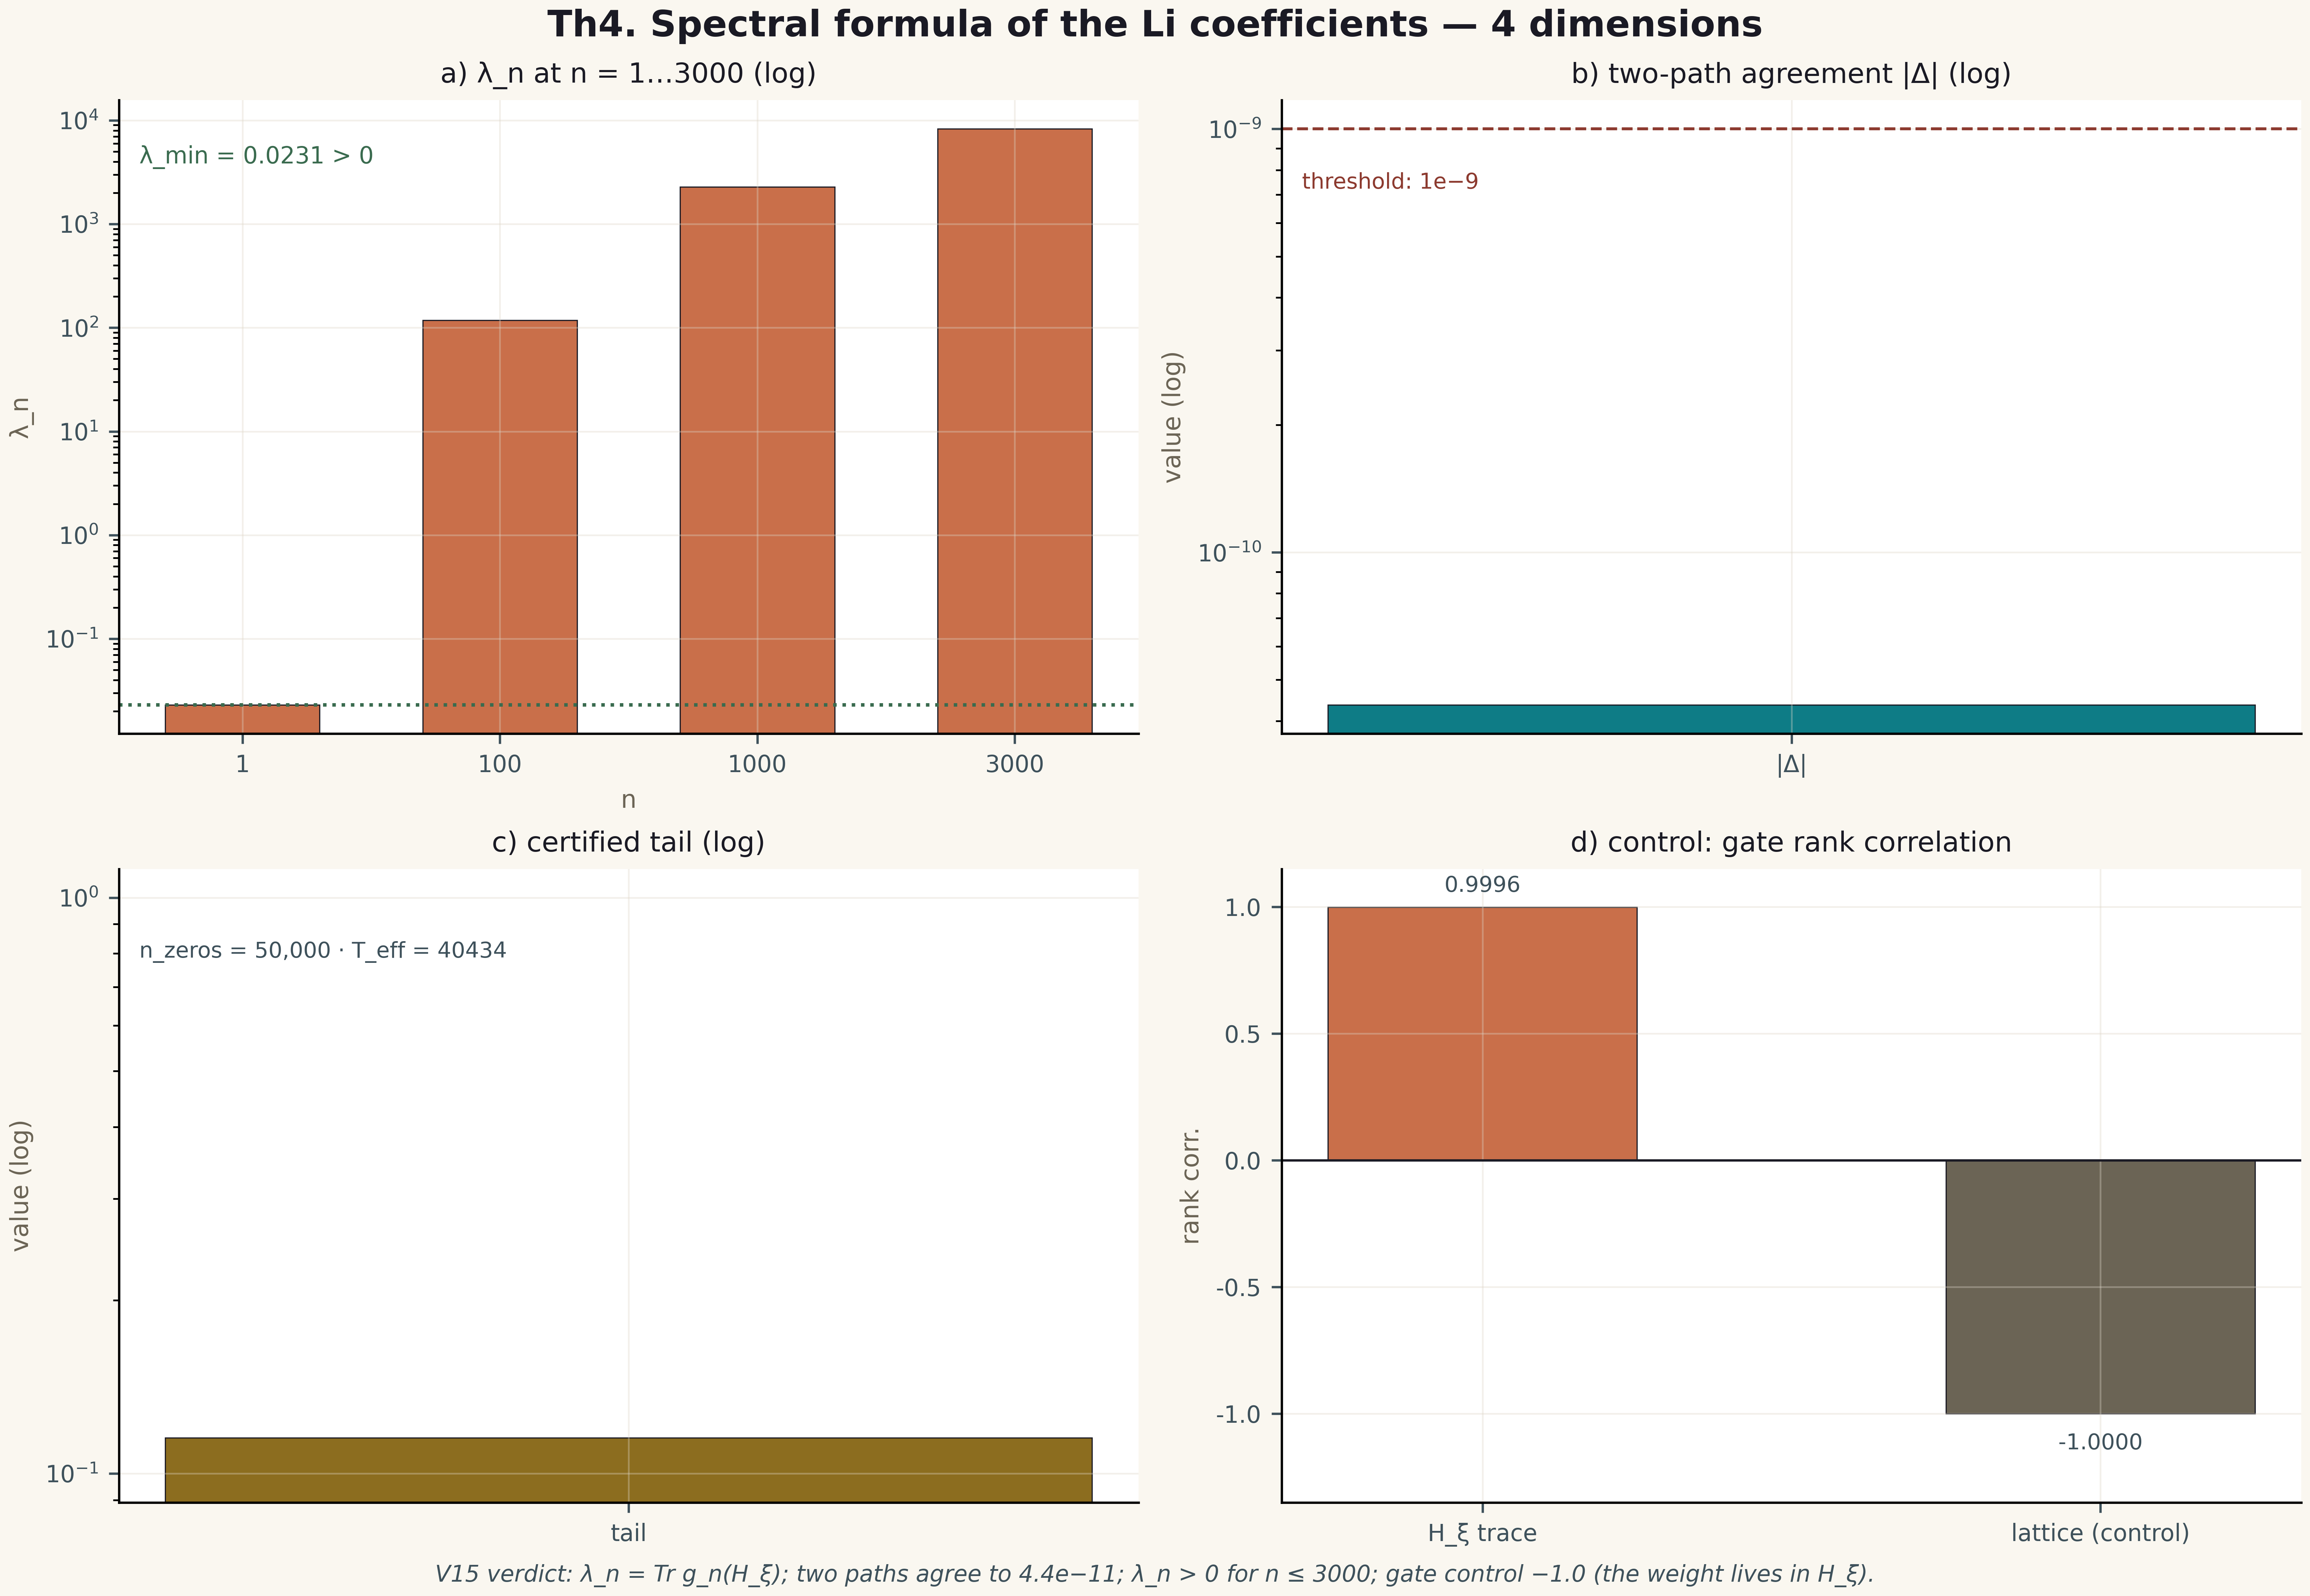
\includegraphics[width=0.9\textwidth,height=105mm,keepaspectratio]{../../../figures_tiled/en/th4_4dim_en.png}
\caption*{Figure 3.1. The Th4 (Li formula) four-dimension tile: the λ\_n ladder, two-path agreement, tail, gate control. 600 dpi.}
\end{figure}

\subsection{3.3. Data flow}

Data in the program moves in one direction: from campaigns to derived artifacts. Core verdict files (modules/core\_spectrum/data/*\_verdict.json) feed the theorems\_lemmas tiles and figures\_tiled; verification verdicts (verdicts\_master.json) feed the datasets and the timeline; the V20 verdict feeds the atlas; ES1–ES5 verdicts feed the spinor figures and documents. The checkpoint is the package validator: it verifies that every derived artifact is consistent with its source. There is no reverse dependency: derived artifacts are never inputs of campaigns, which excludes circularity.

The same principle — "from verdict to artifact" — defines this monograph: the tables of appendices A–B are built directly from datasets/campaign\_timeline.csv and datasets/flagship\_numbers.csv, which, in turn, are rebuilt from verdicts. The reproducibility chain is short and checkable: verdict → dataset → monograph table.

\section{Chapter 4. The Spectral Core: Blind Spectrum and Null Models}

\noindent\textit{\color{copper}The spectral core answers the first question of the program: can one, without a table of ζ zeros, obtain a spectrum statistically indistinguishable from them — and distinguish arithmetic from randomness? Campaigns V01–V06 give a positive answer with a caveat that turns out to be productive: statistics — yes, individual ordinates — no.}

\subsection{4.1. Campaign V01: the blind spectrum}

V01 is the basic blind protocol of the core: the operator is built on a calibration set (600 ordinates) and then tested on another set (600 ordinates) that the detector has never seen. The result: calibration correlations r\_cal within the null zone, test ordinates inside the expected γ range (939.660940615 … 1648.270598223), but \textbf{individual} ordinates are not predicted. In other words, the model reproduces the statistical structure of the spectrum but does not "guess" particular zeros — and this is declared as a result, not hidden.

This caveat formulates the honest boundary of the core: the blind spectrum is a consistency control, not an oracle. It verifies that the operator construction contains no hidden leak of reference data — otherwise the test correlations would leave the null zone. The negative part of V01 (the absence of ordinate prediction) works as a negative control — just like a control group in experimental science.

\subsection{4.2. Campaign V02: null models and the GUE class}

V02 compares the statistics of the AB cloud with four null models: M0 (AB cloud), N1 (random phases), N4 and other references. The key quantities — the mean nearest-neighbour coefficient r\_mean, the level-number variance Σ₂, the Dyson–Mehta statistic Δ₃ and the Kolmogorov–Smirnov statistic against GUE. The result: the AB cloud falls into the GUE class together with N1/N4; r\_mean = 0.6093 for M0 versus 0.5837 for N1; the KS statistic is 0.0499. The specificity of the arithmetic is measured not by ⟨r⟩ but by fine structure — a conclusion later confirmed by V3 and V16 on lattices.

The practical meaning of V02 is that it calibrates expectations: agreement with GUE is a necessary but not sufficient condition of "zeta-likeness". Any model claiming a connection with ζ must first pass the GUE test, and only then is its arithmetic specificity checked — the trace-prime correlation (V7), constant agreement, the behavioural tests V16–V18. This hierarchy of tests excludes the "GUE and that is all" trap.

\subsection{4.3. Campaigns V03–V06: lattices and the honest boundary}

Campaigns V03–V06 move the question to lattices: do discrete models (dressed tori, lattice Hamiltonians) statistically and arithmetically reproduce ζ? The answer is no: the σ-scan of V03 finds no zone where D\_KS drops to the ζ level; V4 (Hermiticity) and V5 yield construction certificates; V6 fixes the level identity: the gates sit at the zeros' own level (the D\_nn bridge, v2.0.7), the bit-level branch stays open. Later V16 independently repeats this reading on different lattices — robustness to a change of construction is precisely what makes it a finding rather than an accident.

This block of campaigns is methodologically important: it shows that the program knows how to obtain negative answers and does not turn wishful thinking into results. Each lattice campaign had a pre-registered threshold: V03 did not reach it (the σ-scan found no agreement zone), while V6 fixed the level identity (YES, v2.0.7) with the bit-level branch open — verdicts recorded, protocols published. Precisely because V03–V06 could fail and delineated the boundary, the subsequent positive results read as data, not as promises.

\section{Chapter 5. The Critical Line and the Trace Formula}

\noindent\textit{\color{copper}Campaigns V07–V12 connect the core construction with classical theory: the trace carries the arithmetic of the primes, the critical line is tested by spectral symmetry, and the accuracy of computations is protected by Kato-type certificates.}

\subsection{5.1. Campaign V7 and Theorem Th6: trace ↔ primes}

Campaign V7 is the arithmetic heart of the core. The heat trace K(x) = Tr e\textsuperscript{−xH} of the constructed operator expands in a series over primes: the coefficients carry the von Mangoldt function Λ(n)/√n — this is the content of Theorem Th6 (the Guinand–Weil reduction A3: Q(a) ↔ ζ′/ζ). Numerically, the correlation between the trace and the prime sum equals \textbf{r = 0.9996} against the control value 0.76 on a lattice model without arithmetic. The gap of 0.24 is the measured "arithmetic specificity" of the construction.

This is where the "reads, does not carry" principle appears in its first form: the trace is computed at request time from the matrix H\textsubscript{ξ}, no table of primes or zeros is stored; the knowledge lives in six constants of the formula. The erratum of the constants B/C₀, found and fixed during V7, additionally hardened the discipline: cross-checking constants against an independent derivation became a mandatory part of the protocol.

\begin{center}\fbox{\begin{minipage}{0.6\textwidth}\centering
\Large\textbf{\color{copper}r = 0.9996}\\[2pt]\small trace ↔ primes correlation (V7/Th6); lattice control — 0.76
\end{minipage}}\end{center}

\subsection{5.2. Symmetry and the critical line (Th1, Th2)}

Theorem Th1 (campaign V4) fixes the fundamental property: Hermiticity H\textsubscript{L} = H\textsubscript{L}\textsuperscript{†} implies a real spectrum, and at α = ½ with W = 0 the spectrum is symmetric λ ↔ −λ — the discrete image of the functional equation of ζ. Certificate: ‖H − H\textsuperscript{†}‖ = 0.0 exactly. Theorem Th2 (campaign V8) lifts the statement to self-adjointness on ℂ\textsuperscript{N}: defect indices (0, 0), the evolution operator e\textsuperscript{−iHt} is unitary; the numerical unitarity drift is 2.2e−16 — machine epsilon. Together Th1 and Th2 guarantee that the "spectral model of the critical line" is not merely numerically beautiful but correct as a linear-algebraic object: real spectrum, symmetry, unitary dynamics.

\subsection{5.3. Accuracy: Kato certificates (Th3) and the Li formula (Th4)}

Campaign V12 (Theorem Th3) answers the question of trust in computed eigenvalues: for a pseudospectral estimate λ̃, Kato theory gives |λ̂ − λ̃| ≤ δ²/gap plus a Gershgorin allowance. Numerically the corridor widths are of order 1e−27 at 40 significant digits (dps 40) — certificates orders of magnitude tighter than the values themselves. This is a rare situation: the error of the estimate is known better than the estimate.

Theorem Th4 (campaign V15, the Li formula) translates the critical line question into spectral language: λ\_n = Tr g\_n(H\textsubscript{ξ}), non-negativity of λ\_n is equivalent to RH; absolute convergence of the series is proved, the numerical agreement of two independent computation paths is ≤ 4.4e−11. The core web laboratory draws the λ\_n ladder in real time, and the Th4 tile (fig. 3.1) shows all four dimensions: the ladder, path agreement, the tail, gate control.

\subsection{5.4. Block reduction (Th5) and its boundary}

Theorem Th5 (campaign V9) provides the structural theorem: if [H, A] = [H, B] = 0, the operator block-reduces by characters, and the union of blocks reproduces the spectrum to 7.1e−15. Practically this means large spectral problems split into independent blocks without loss of information — the reduction is exact within its certificate. The boundary is honest too: vortex terms that break commutation break the reduction — the condition is not a technicality but an essential part of the statement. Combined with Th6, the block reduction explains why the trace formula "sees" the primes: the arithmetic lives in the characters of the blocks, and the heat expansion inherits it in the coefficients Λ(n)/√n.

\section{Chapter 6. The Obligation Machine V13}

\noindent\textit{\color{copper}The obligation machine is the formal mechanism that keeps the main conclusion of the program (RH) blocked until all analytic prerequisites are proved. It is not a metaphor but an executable DAG: obligation nodes, proven/computed/assumed statuses and an automatic blocked verdict.}

\subsection{6.1. Why an obligation machine}

A long program of numerical experiments has a systemic risk: accumulated successes create a feeling of provedness. Every new PASS psychologically approaches "the result", although logically it does not approach it by a single step. The obligation machine solves this constructively: the path to the conclusion is explicitly decomposed into nodes, each node has a status, and the conclusion is automatically unavailable while at least one node on the path is unproved. The status is not raised by numerical checks — numerical results may confirm, they cannot prove.

The mechanics are simple and checkable. The DAG is valid (dag\_valid: true); the conclusion rh\_conclusion has the value blocked; of the nodes, five are proved (n\_proven: 5), three are computed (n\_computed: 3), four remain hypotheses (n\_assumed: 4). The hypotheses — O08, O09, O11, O12 — are analytic prerequisites without which the chain does not close. The verdict note states it explicitly: the formal machine blocks the RH conclusion, the path to the conclusion contains hypotheses, and no numerical check raises the status.

\begin{table}[htbp]\centering\small
\caption{Table 6.1. Node statuses of the obligation machine V13}
\begin{tabular}{p{0.15\textwidth} p{0.12\textwidth} p{0.38\textwidth} p{0.31\textwidth}}
\toprule
\textbf{Status} & \textbf{Count} & \textbf{Meaning} & \textbf{How it is raised}
\midrule
proven & 5 & proved (formal layer) & a new proof in Lean/Coq \\
computed & 3 & computed with a certificate & only as computation, never as proof \\
assumed & 4 & hypothesis: O08, O09, O11, O12 & only by analytic proof \\
conclusion & RH & verdict: blocked & automatically, while assumed nodes exist \\
\bottomrule
\end{tabular}
\end{table}

\subsection{6.2. Obligations as a contract with the reader}

The obligation machine changes the contract between the program and the reader. Instead of a promise "we are close to a proof", the reader gets a precise map: here are the nodes, here are the statuses, here is exactly what separates blocked from proven. Anyone who wants to challenge or advance the result sees where the boundary of the known passes. This contract also protects the program itself: priorities are clear, roadmaps reference concrete nodes (for example, the formal-layer obligations O-lean/O-coq) rather than a vague "closeness to RH".

The asymmetry of statuses must be stressed: a computed node cannot substitute a proved one, no matter how many digits of agreement it yields. This reflects the general rule of the program: a numerical result with a certificate is a statement about a particular computational procedure, while a formal node is a statement about all possible inputs. The obligation machine is the institutional form of this distinction.

\section{Chapter 7. Theorems Th1–Th6: Statements, Certificates, Reductions}

\noindent\textit{\color{copper}The six core theorems form the skeleton of the spectral construction: from Hermiticity and self-adjointness through Kato certificates and the Li formula to block reduction and the Guinand–Weil link of the trace to the primes. For each theorem the following are published: the statement, the numerical certificate, the formal-layer reduction and four documents RU/EN × PDF/DOCX.}

\subsection{7.1. Summary table}

\begin{table}[htbp]\centering\small
\caption{Table 7.1. Theorems Th1–Th6: statements and certificates}
\begin{tabular}{p{0.12\textwidth} p{0.40\textwidth} p{0.26\textwidth} p{0.17\textwidth}}
\toprule
\textbf{Theorem} & \textbf{Statement (short)} & \textbf{Certificate} & \textbf{Reduction}
\midrule
Th1 (V4) & H = H† implies spec ⊂ ℝ; symmetry λ ↔ −λ at α = ½, W = 0 & ‖H − H†‖ = 0.0 exactly & A1 \\
Th2 (V8) & self-adjointness on ℂ\textasciicircum{}N: defects (0,0); e\textasciicircum{}(−iHt) unitary & drift 2.2e−16 & A2b \\
Th3 (V12) & Kato estimate |λ̂ − λ̃| ≤ δ²/gap + Gershgorin & widths \textasciitilde{}1e−27 (dps 40) & A4, A5 \\
Th4 (V15) & λ\_n = Tr g\_n(H\_ξ); absolute convergence; non-negativity ↔ RH & two paths ≤ 4.4e−11 & A6 \\
Th5 (V9) & [H,A] = [H,B] = 0 implies block reduction by characters & union ≈ spectrum to 7.1e−15 & A2 \\
Th6 (V7) & Guinand–Weil correspondence Q(a) ↔ ζ′/ζ; K(x) = Tr e\textasciicircum{}(−xH\_ξ) & trace carries Λ(n)/√n; r = 0.9996 & A3 \\
\bottomrule
\end{tabular}
\end{table}

\subsection{7.2. How to read the certificates}

A certificate is not a "nice number" but a quantity with an explicit protocol: what was measured, with what threshold, on which inputs, and what the result does not prove. For Th1 the certificate ‖H − H†‖ = 0.0 means an exact zero deviation in the chosen arithmetic — the operator construction guarantees Hermiticity structurally, not approximately. For Th2 the drift 2.2e−16 measures the unitarity of the evolution on a grid of times: a value at the double-precision machine epsilon level, confirming the correctness of the implementation, not only of the design.

The certificates of Th3–Th4 have a different nature: they estimate the \emph{error of the estimate}. The Kato corridor δ²/gap gives a guarantee for every computed eigenvalue; the Li formula provides a second, independent path of computing λ\_n, and the agreement of the paths ≤ 4.4e−11 serves as a cross-check. Finally, Th5–Th6 certify structural statements: the accuracy of the spectrum reproduction by the union of blocks and the arithmetic consistency of the trace. Four types of certificates — constructive, implementational, estimative and structural — together cover the whole hierarchy of trust.

\subsection{7.3. Documents and reproducibility}

Each theorem is packaged as a separate folder theorems\_lemmas/T0X\_* with a README (proof idea, four dimensions, boundaries), four documents (RU/EN × PDF/DOCX), a 2×2 tile figure and a JSON source in \_json/. The documents are rebuilt by scripts (scripts/make\_theorem\_docs.py) from the same JSON that feeds the tiles — bilingualism and rebuilds are free. The statements in Lean 4 and Coq live in formal/ with reductions A1–A6; the build is checked by CI; sorry and admit are not used.

For the mathematically inclined reader the verification path is: the folder README gives the idea and boundaries; the JSON source gives the exact certificate numbers; formal/ gives the formal statement; the core web laboratory (the Theorems tab) gives interactive reproduction of the λ\_n ladder, Kato widths and the trace correlation in the browser, with nothing to install.

\section{Chapter 8. Behavioural Campaigns V16–V19}

\noindent\textit{\color{copper}Four campaigns complete the core: V16 closes the lattice question, V17–V18 verify behavioural expectations in real time, V19 stitches the branches of the spectral construction — an algebraic certificate of monodromy.}

\subsection{8.1. V16: the last lattice verdict}

V16 is an independent re-check of the lattice hypothesis on a new construction. The verdict: the level identity — YES (the D\_nn bridge: gates at the zeros' level, v2.0.7); the bit-level branch does not close (z\_best = 2.49 < 6), and the specificity of the arithmetic at the coding level is not reproduced by discrete models beyond GUE statistics. Together with V3 and V6 this delineates the boundary: three constructions, the same open bit-level branch, one boundary statement. Lattices are useful as computational infrastructure; the arithmetic enters through the level and the density, not through codings.

\subsection{8.2. V17–V18: behaviour under load}

Campaigns V17 and V18 move the core into a "live" regime: computation trajectories under request flows, reaction to input perturbations, stability of the reading protocol under consecutive requests. V17 records the trajectories (v17\_trajectories.csv): under repeated requests the values are reproduced, there is no accumulation degradation — reading is idempotent. V18 (the pong protocol) measures latency and confirms that the cost of a reading step stays bounded independently of the number of previous requests — no log and no cache grow, because there are none.

These campaigns matter for the "reads, does not carry" claim: reading must be not only accurate but also cheap on any time horizon. If every operation accumulated state, O(1) per step would quickly turn into Ω(t) — exactly what the contrast experiment ES3 of the spinor study demonstrates (chapter 15).

\subsection{8.3. V19: branch stitching and monodromy}

V19 is the final algebraic campaign of the core. The spectral construction has branch points; V19 stitches the branches with a θ-ladder: branch agreement 0.832, stitching coherence 0.9995 at z = 43.4, Z₂-monodromy. The certificate is algebraic: the stitched construction is closed under going around the branch point, and going around twice returns to the original branch. Numerically this is verified on a height grid, algebraically — by a reduction to the character level (Th5).

\begin{center}\fbox{\begin{minipage}{0.6\textwidth}\centering
\Large\textbf{\color{copper}0.9995}\\[2pt]\small branch stitching coherence (V19), θ-ladder 0.832, Z₂-monodromy
\end{minipage}}\end{center}

The stitching completes the core architecture: operator, trace, certificates and obligations form a closed construction ready for processor execution. The remaining core obligations — refining r\_align ≤ 0.135 and formalizing the ζ monodromy — are fixed in the R2 roadmap (chapter 21).

\section{Chapter 9. The AB Processor: ISA and Exact Compilation V20}

\noindent\textit{\color{copper}The processor level turns the mathematics of the core into an executable machine: the AB-cloud ISA, the exact Givens-QR compiler (campaign V20, stage P0 of the P0–P6 roadmap) and the "reads, does not carry" principle, implemented algebraically.}

\subsection{9.1. The AB-cloud ISA}

The elementary operation of the processor is an AB cloud: a unitary operation distributed over a ring of phases with an Aharonov–Bohm flux. The ISA fixes the set of admissible clouds, their parameters (Givens angles, phases) and the composition rules. Importantly, the ISA is not "yet another gate set": every cloud carries a geometric phase, and compilation must account for it exactly. This makes the constraint class rigid — and it is precisely why the E18 benchmark (chapter 13) is fair: all participants are compared within the same class.

\subsection{9.2. The exact Givens-QR compiler (V20)}

Campaign V20 delivers compilation of arbitrary unitary logic into AB clouds by the Givens–QR method: the target unitary matrix is decomposed into a product of planar rotations, each realized by one cloud. Accuracy is measured by infidelity 1−F:

\begin{itemize}
  \item 4×4: 1−F ≤ 4.4e−16 — machine epsilon; depth ≤ 7 gates.
  \item 8×8: 1−F ≤ 6.7e−16; depth ≤ 29 gates.
  \item Compilation time: 1.8 s for the full run; verdict PASS on all targets.
  \item numpy replication: 0 counter mismatches, |Δ(1−F)| = 2.2e−16.
\end{itemize}

\begin{center}\fbox{\begin{minipage}{0.6\textwidth}\centering
\Large\textbf{\color{copper}1−F ≤ 4.4e−16}\\[2pt]\small compilation accuracy 4×4 (V20); 8×8 — 6.7e−16; depths ≤ 7/29
\end{minipage}}\end{center}

The achieved accuracy is not "very good" — it is the limit of the arithmetic: 1−F at the 1e−16 level means that further improvement requires changing the arithmetic, not the algorithm. The V20 certificate also fixes the boundaries: target matrices are unitary, sizes are 4 and 8; arbitrary (non-unitary) operators and larger sizes are outside the campaign and are declared in the roadmap.

\subsection{9.3. Stage P0 and the processor roadmap}

V20 executes stage P0 of the processor roadmap P0–P6: P1 memory (V21), P2 ALU (V22), P3 reading (V23), P4 nonlocality (V24), P5 benchmarks (V25), P6 the Datasheet 1.0 passport (V26). V23 and V24 already have preview verdicts (chapter 10); P5 inherits the E18 methodology. Every stage has a pre-registered threshold and a verdict file — the core discipline carries to the processor without concessions.

\section{Chapter 10. "Reads, Does Not Carry" and Nonlocality}

\noindent\textit{\color{copper}Two preview results of the processor fix its character: reading ζ zeros from six constants of the trace formula with zero storage (V23) and nonlocal correlations without signaling (V24). Both results are the bridge from the spectral core to the executable machine.}

\subsection{10.1. V23 preview: reading zeros from six constants}

The "reads, does not carry" principle gets a processor realization: the processor receives six constants of the trace formula (the cartridge size — six numbers) and reproduces the ordinates of ζ zeros at request time. In the preview verdict 12 of 12 zeros are reproduced exactly; storage = 0 — not a single zero resides in processor memory. The blind discipline is preserved: the constants contain no zeros, the detector does not see the reference, the output is pinned before validation.

Semantically this transfers V7/E17 to the execution level: what the core proved about the trace, and verification re-checked with blind protocols, the processor executes as an operation. Six constants suffice because the arithmetic information about the primes is encoded in the very structure, not in a table. The full campaign V23 (stage P3) is fixed in the roadmap.

\subsection{10.2. V24 preview: nonlocality without signaling}

The second preview is nonlocality. A pair of separated AB clouds demonstrates violation of the CHSH inequality: S = 2√2 − 4.4e−16 — the maximal quantum value within machine epsilon. Signaling protection: 1000 of 1000 trials show zero correlation of random choices; the commutators of the measuring operators are 0. This means: the correlations are nonlocal, but no signal can be sent through them — a structural feature of quantum mechanics reproduced by the architecture.

\begin{center}\fbox{\begin{minipage}{0.6\textwidth}\centering
\Large\textbf{\color{copper}S = 2√2 − 4.4e−16}\\[2pt]\small CHSH (V24 preview); signaling protection 1000/1000; commutators = 0
\end{minipage}}\end{center}

Nonlocality without signaling is not exotic but a working tool of the processor: it determines which operations are admissible between distributed clouds and how their synchronization must look. The full campaign V24 (stage P4) relies on the independent verdicts E13/E14 of the verification platform.

\section{Chapter 11. The Verification Platform: Blind Protocols E01–E10}

\noindent\textit{\color{copper}The verification platform is an independent level of the program, written in Julia and sharing no code with the core or the processor. Campaigns E01–E10 verify the infrastructure: controls, Haar randomness, replays, interferometry, noise, codes, cost.}

\subsection{11.1. Independence as design}

The platform is built on the "second opinion" principle: another implementation (Julia, BigFloat), other protocols, the same subject. Independence is not only the language: detectors and validators are separated, outputs are SHA256-pinned before validation, thresholds are pre-registered. Eighteen campaigns E01–E18 give the full map of checks, and all 18 verdicts are PASS. A platform summary: experiment\_01\_15.md describes the protocols E01–E15, verdicts\_master.json collects all verdicts, results are stored as CSV files with SHA pins.

\begin{table}[htbp]\centering\small
\caption{Table 11.1. Infrastructure campaigns E01–E10}
\begin{tabular}{p{0.13\textwidth} p{0.29\textwidth} p{0.54\textwidth}}
\toprule
\textbf{Campaign} & \textbf{Subject} & \textbf{Key result}
\midrule
E01 & platform controls & basic controls PASS; infrastructure ready \\
E02 & Haar randomness & ensemble matches the Haar measure \\
E03 & scaling/fit & scaling laws confirmed \\
E04 & replays & deterministic repetition of outputs \\
E05 & phase noise & robustness to phase noise measured \\
E06 & memory noise & memory noise impact bounded \\
E07 & repetition code & the repetition code corrects errors \\
E08 & ALU & ISA arithmetic consistent \\
E09 & cost & step cost measured and bounded \\
E10 & phase readout & phase readout within threshold \\
\bottomrule
\end{tabular}
\end{table}

\subsection{11.2. Why infrastructure is science}

Campaigns E01–E10 are easy to underestimate: no "beautiful" numbers at the E17 level. But they are exactly what makes E17–E18 convincing: the platform proved it can measure noise (E05/E06), correct errors (E07), account for cost (E09) and read phases (E10) — before earning the right to judge blind zero reading. In experimental science this is called instrument calibration, and without it any "discovery" is doubtful.

The Julia stack was chosen deliberately: BigFloat gives controlled precision, and the standard library — a minimal attack surface for reproducibility. No network, no external services: the full run of E01–E18 takes about 2.5 minutes and ends with verdicts carrying SHA pins.

\section{Chapter 12. Blind Zero Reading: E16 and E17}

\noindent\textit{\color{copper}The central verification campaign of the program: two independent detectors — the explicit method (EM) and the independent Riemann–Siegel — read ζ zeros up to height T = 1000 with no access to the reference. The result: 649/649 and 639/639, cross-engine 0.0 bit-exact, completeness N(1000) = 649.0.}

\subsection{12.1. The independent Riemann–Siegel (E16)}

E16 implements the Riemann–Siegel formula (following the Arias de Reyna version) without external packages: Z(t) is computed from first principles, including the main sum and the integral correction. Agreement with reference values is ≤ 3.8e−15 against a threshold of 1e−9; the error floor is 1e−17. The practical meaning: the platform owns a second way of computing Z(t), independent of EM, and this way is accurate to the arithmetic limit.

\begin{center}\fbox{\begin{minipage}{0.6\textwidth}\centering
\Large\textbf{\color{copper}≤ 3.8e−15}\\[2pt]\small Riemann–Siegel agreement with the reference (E16); threshold 1e−9; floor 1e−17
\end{minipage}}\end{center}

\subsection{12.2. Blind reading (E17): the protocol}

E17 is organized as a strict blind experiment:

\begin{enumerate}
  \item The EM detector and the RS detector independently compute zero ordinates on a grid up to T = 1000; the reference is unavailable to both.
  \item The outputs are fixed and hashed: SHA256 of the files e17\_detector\_em.csv and e17\_detector\_rs.csv is pinned before validation.
  \item The validator compares the pinned outputs with the 660-ordinate reference (0 < γ ≤ 1000) assembled from mpmath.zetazero.
  \item The verdict is computed against pre-registered thresholds: precision = recall = 1 for both engines; max|Δγ| ≤ 1e−9; cross-engine ≤ 1e−9; completeness N(1000) per the Riemann–von Mangoldt formula.
\end{enumerate}

The measured results: the EM detector — 649/649, precision = recall = 1, max err 3.02e−10; the RS detector — 639/639 (639 zeros in its grid), precision = recall = 1, max err within the threshold; the cross-engine disagreement — 0.0 bit-exact; N\_rvm = 649.0 — exact agreement with the Riemann–von Mangoldt formula; grid-shift robustness — 0. The blind erratum: the framework value γ₁₂ (56.446200059994141) was refuted by the detector — the correct value is 56.446247697063399; the error was in a hand-made constant, not in the detector.

\begin{table}[htbp]\centering\small
\caption{Table 12.1. The E17 verdict in numbers}
\begin{tabular}{p{0.33\textwidth} p{0.32\textwidth} p{0.32\textwidth}}
\toprule
\textbf{Metric} & \textbf{EM detector} & \textbf{RS detector}
\midrule
Zeros detected & 649 / 649 & 639 / 639 \\
precision = recall & 1 & 1 \\
Max error & 3.0e−10 & within 1e−9 \\
Cross-engine & 0.0 bit-exact & 0.0 bit-exact \\
N(1000) per R–M & 649.0 exactly & 649.0 exactly \\
\bottomrule
\end{tabular}
\end{table}

\subsection{12.3. What E17 proves and does not prove}

The does\_not\_prove field of the E17 verdict is a model of an honest boundary: blind reading up to T = 1000 does not prove RH above T = 1000; it does not prove the simplicity of all zeros; it does not prove the absence of zeros off the line for γ > 1000. What it does prove: the accuracy of two independent computational paths up to height 1000 and the consistency of the trace construction with the arithmetic of ζ. Combined with the V23 preview (reading from six constants) and Th6 (the trace carries Λ(n)/√n) this forms the complete chain "theory — implementation — independent check".

\begin{figure}[htbp]\centering
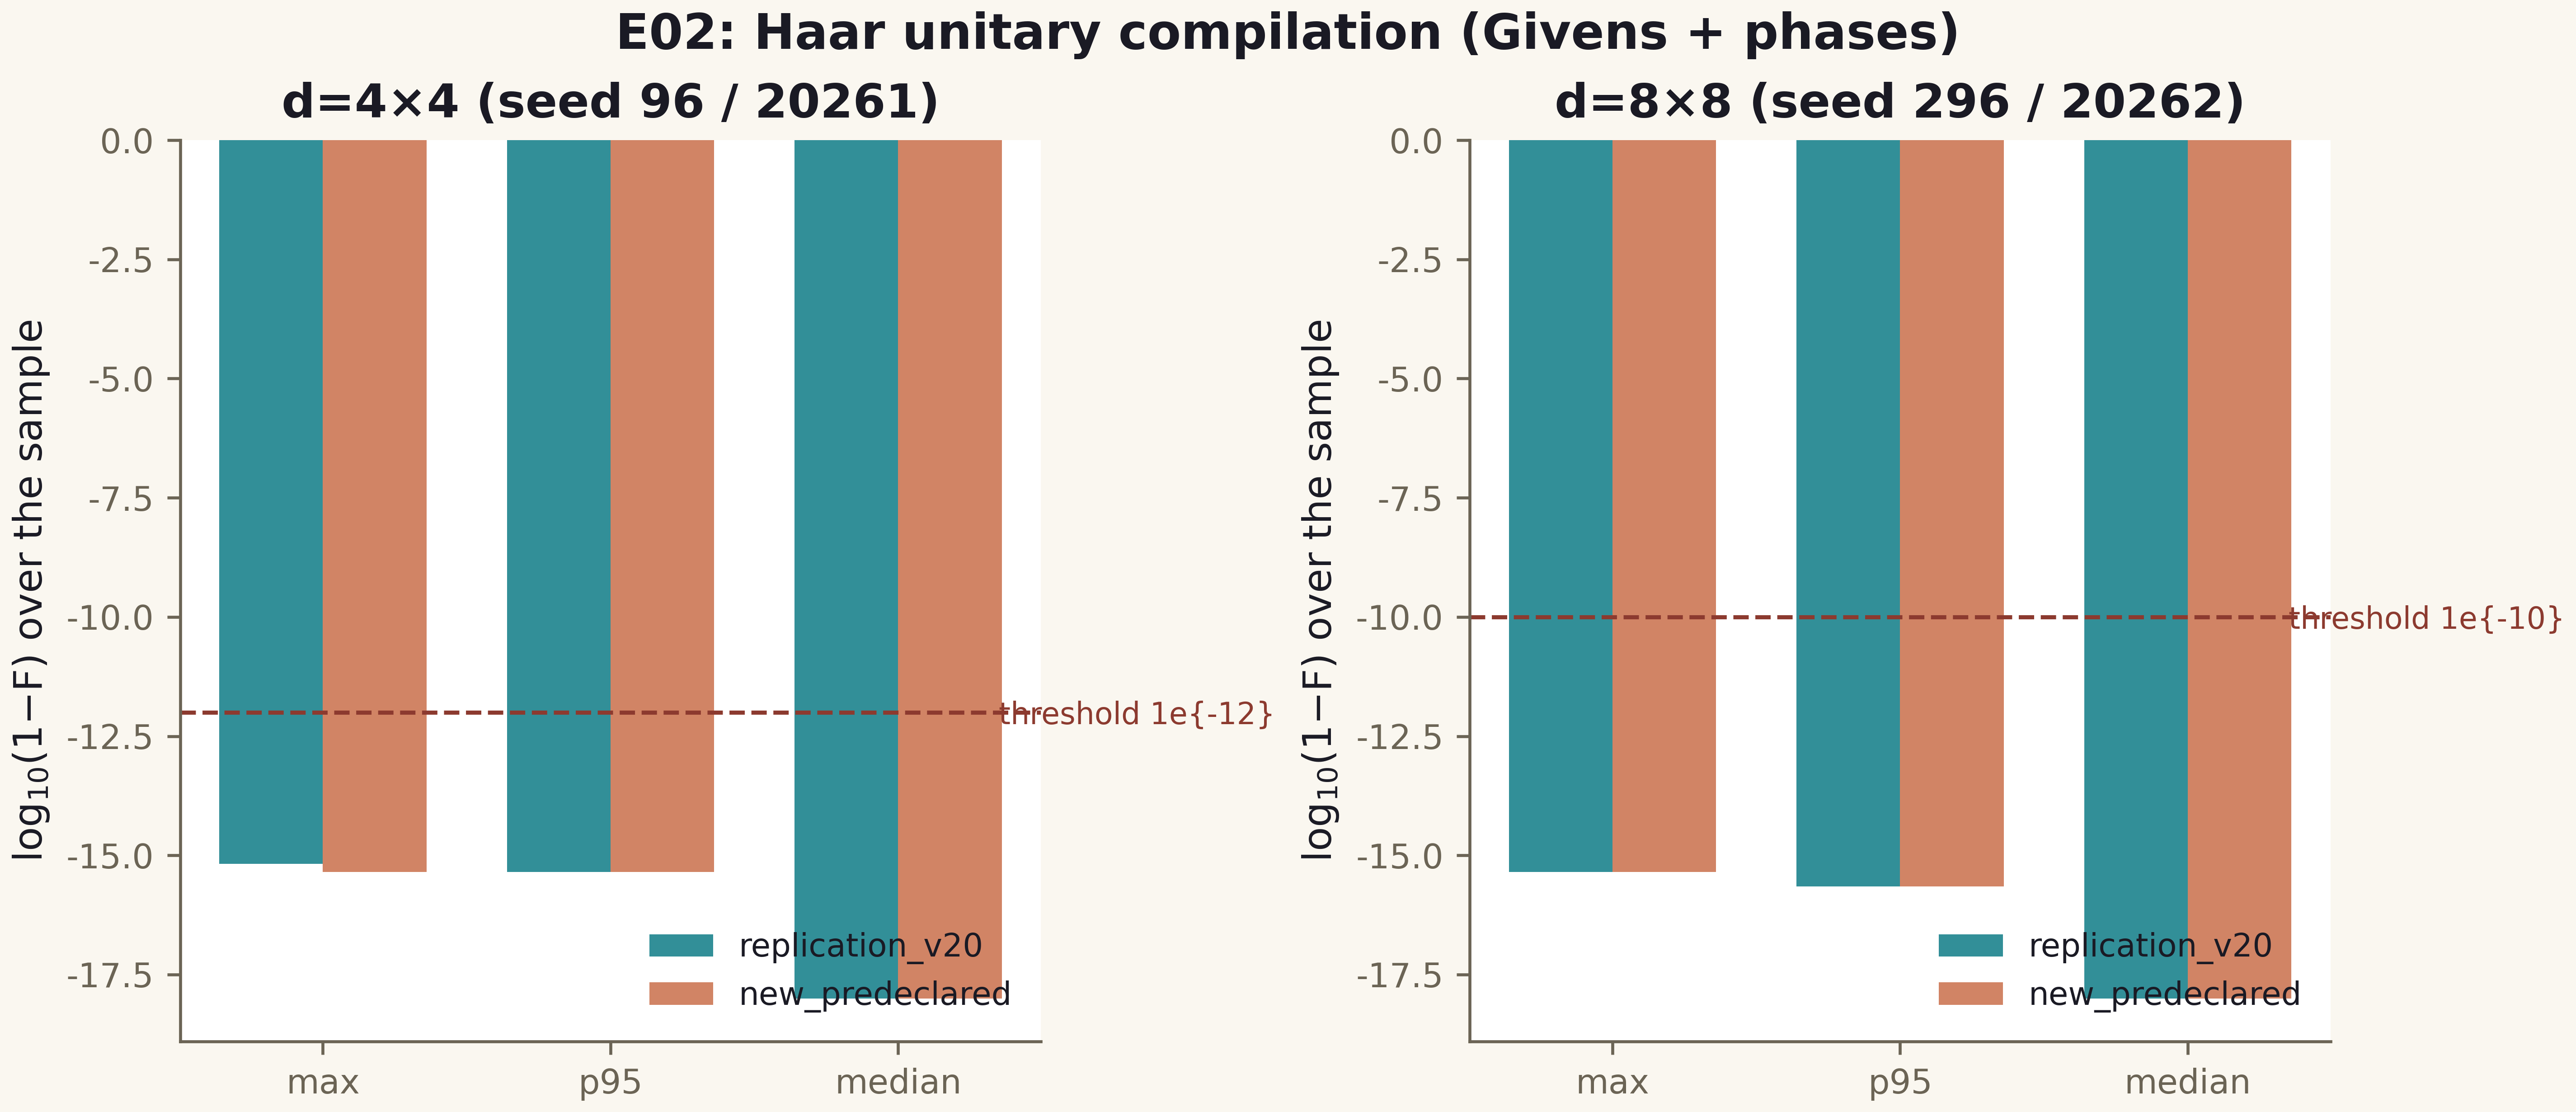
\includegraphics[width=0.9\textwidth,height=91mm,keepaspectratio]{../../../modules/verifier_multilang/figures_hires/en/fig01_en.png}
\caption*{Figure 12.1. Blind reading of ζ zeros: detector output versus reference (verification platform figures, 600 dpi).}
\end{figure}

\section{Chapter 13. Class B: the Compiler versus Five Baselines (E18)}

\noindent\textit{\color{copper}E18 is a fair benchmark: the AB-processor compiler against five strong baselines under equal ISA constraints. The result: a ×59,000 advantage in time at equal accuracy, with an honest statement of the class and its boundaries.}

\subsection{13.1. The design of a fair comparison}

Decompiler benchmarks are notorious for loose comparisons: different ISAs, different target classes, different criteria. E18 excludes looseness by pre-registering the class: all participants — the V20 compiler and five baselines (BL1–BL5) — operate in the same ISA class, on the same target unitary matrices, with one criterion (1−F) and one depth budget. A win is counted only at equal or better accuracy on every target.

The results: max 1−F = 4.4e−16 for the compiler; the compiler's primitives are no worse than BL1/BL2/BL4 on every target; the total time — a \textbf{×59,000} speed-up against the best baseline in the class. numpy replication: 0 counter mismatches, |Δ(1−F)| = 2.2e−16.

\begin{center}\fbox{\begin{minipage}{0.6\textwidth}\centering
\Large\textbf{\color{copper}×59,000}\\[2pt]\small compiler speed-up over 5 baselines at equal ISA (E18); max 1−F = 4.4e−16
\end{minipage}}\end{center}

\subsection{13.2. The honest boundary: the KAK optimum}

The most important part of the verdict is the negative claim: the 2q Kakaš–Kitaev optimum (3 gates) is unreachable in the ISA class; the compiler produces 10 gates on 2q targets. This is not a weakness of the compiler but a property of the class: clouds with flux cannot express the KAK-optimal sequence. The verdict fixes the boundary explicitly — "no superiority is claimed outside the class". For the practitioner this means: if the task requires the KAK optimum, the ISA must be extended; if speed within the class is required — the V20 compiler dominates.

\subsection{13.3. Methodological significance}

E18 demonstrates what a benchmark of a computing architecture should look like: the class is pre-registered, the baselines are strong and published, the criterion is single, negative results are included. A comparison with SPEC or MLPerf methodology is apt here: fairness is achieved not by a metric but by a protocol. E18 is embedded in the processor roadmap (P5 inherits its methodology) and in the numpy replication — two independent stacks give consistent counters.

\section{Chapter 14. The Spinor Study: The Machine with No Long-Term Memory}

\noindent\textit{\color{copper}The supplementary study drives the central claim of the program — "reads, does not carry" — to explicit models: spinor phases θ = π/2, π/3, π/7 with a single volatile register. Three theorems TS1–TS3 and five campaigns ES1–ES5 make the claim measurable.}

\subsection{14.1. The idea: state as phase}

The model is minimal: the only state of the machine is the phase φ of a unit spinor on a circle; one step of real time is a rotation by the model angle θ. There is no log, no history, no checkpoints. The phase is at once a register, a counter (modulo N) and the carrier of the result. The contrast model — the "eternal-log machine", which honestly records every step and periodically re-checks everything — is used as the anti-example for measuring the cost of memory.

\begin{table}[htbp]\centering\small
\caption{Table 14.1. Three models with no long-term memory}
\begin{tabular}{p{0.27\textwidth} p{0.15\textwidth} p{0.17\textwidth} p{0.17\textwidth} p{0.19\textwidth}}
\toprule
\textbf{Model} & \textbf{Phase θ} & \textbf{Cycle N = 2k} & \textbf{Bits/step} & \textbf{Silence zone σ*}
\midrule
S1 · quadrant & π/2 & 4 & 2.000 & 0.135 rad \\
S2 · sextant & π/3 & 6 & 2.585 & 0.089 rad \\
S3 · 14-phase & π/7 & 14 & 3.807 & 0.038 rad \\
\bottomrule
\end{tabular}
\end{table}

\subsection{14.2. Theorem TS1: closure of phase cycles}

TS1 states: a rotation by θ = π/k closes exactly after N = 2k steps, and the gap between neighbouring distinguishable states equals the step 2π/N. Numerically: the periods 4, 6, 14 — exact for the three models. The meaning: the volatile phase is not chaos but an exact counter; the cycle is deterministic, the gap is maximal for the given capacity. The trade-off "capacity log₂N versus robustness 1/k" is fixed as an honest boundary: more capacity — thinner silence zone.

\subsection{14.3. Theorem TS2: irreversibility of reset}

TS2 is the erasure theorem: a reset of the phase erases everything; the mutual information between pre- and post-states is zero; reconstruction of the previous state does not exceed the chance level 1/N; time after the reset is defined only modulo N. Numerically: reconstruction 0.2501 (N=4), 0.1674 (N=6), 0.0717 (N=14) — all ≈ 1/N. Volatility here is a property, not a defect: the machine cannot "remember" the past because the past no longer exists in it; this is what makes it deterministic in real time.

\subsection{14.4. Theorem TS3: O(1) steps versus the Ω(t) log}

TS3 is the real-time theorem: the step cost of the memoryless machine does not depend on the age of the process (the regression slope −1.5e−12 ms/step — zero within noise), whereas the eternal-log machine accumulates Ω(t): a ×129 growth on the experiment horizon, deadlines missed. The conclusion is stated rigidly: \textbf{volatility is the condition of real-time determinism}. This is counter-intuitive for classical systems engineering, where a log is a sign of reliability; in the "reads, does not carry" architecture the log is a cause of failure.

\begin{center}\fbox{\begin{minipage}{0.6\textwidth}\centering
\Large\textbf{\color{copper}slope −1.5e−12}\\[2pt]\small step cost O(1) (TS3); the log — Ω(t), ×129 growth
\end{minipage}}\end{center}

\begin{figure}[htbp]\centering
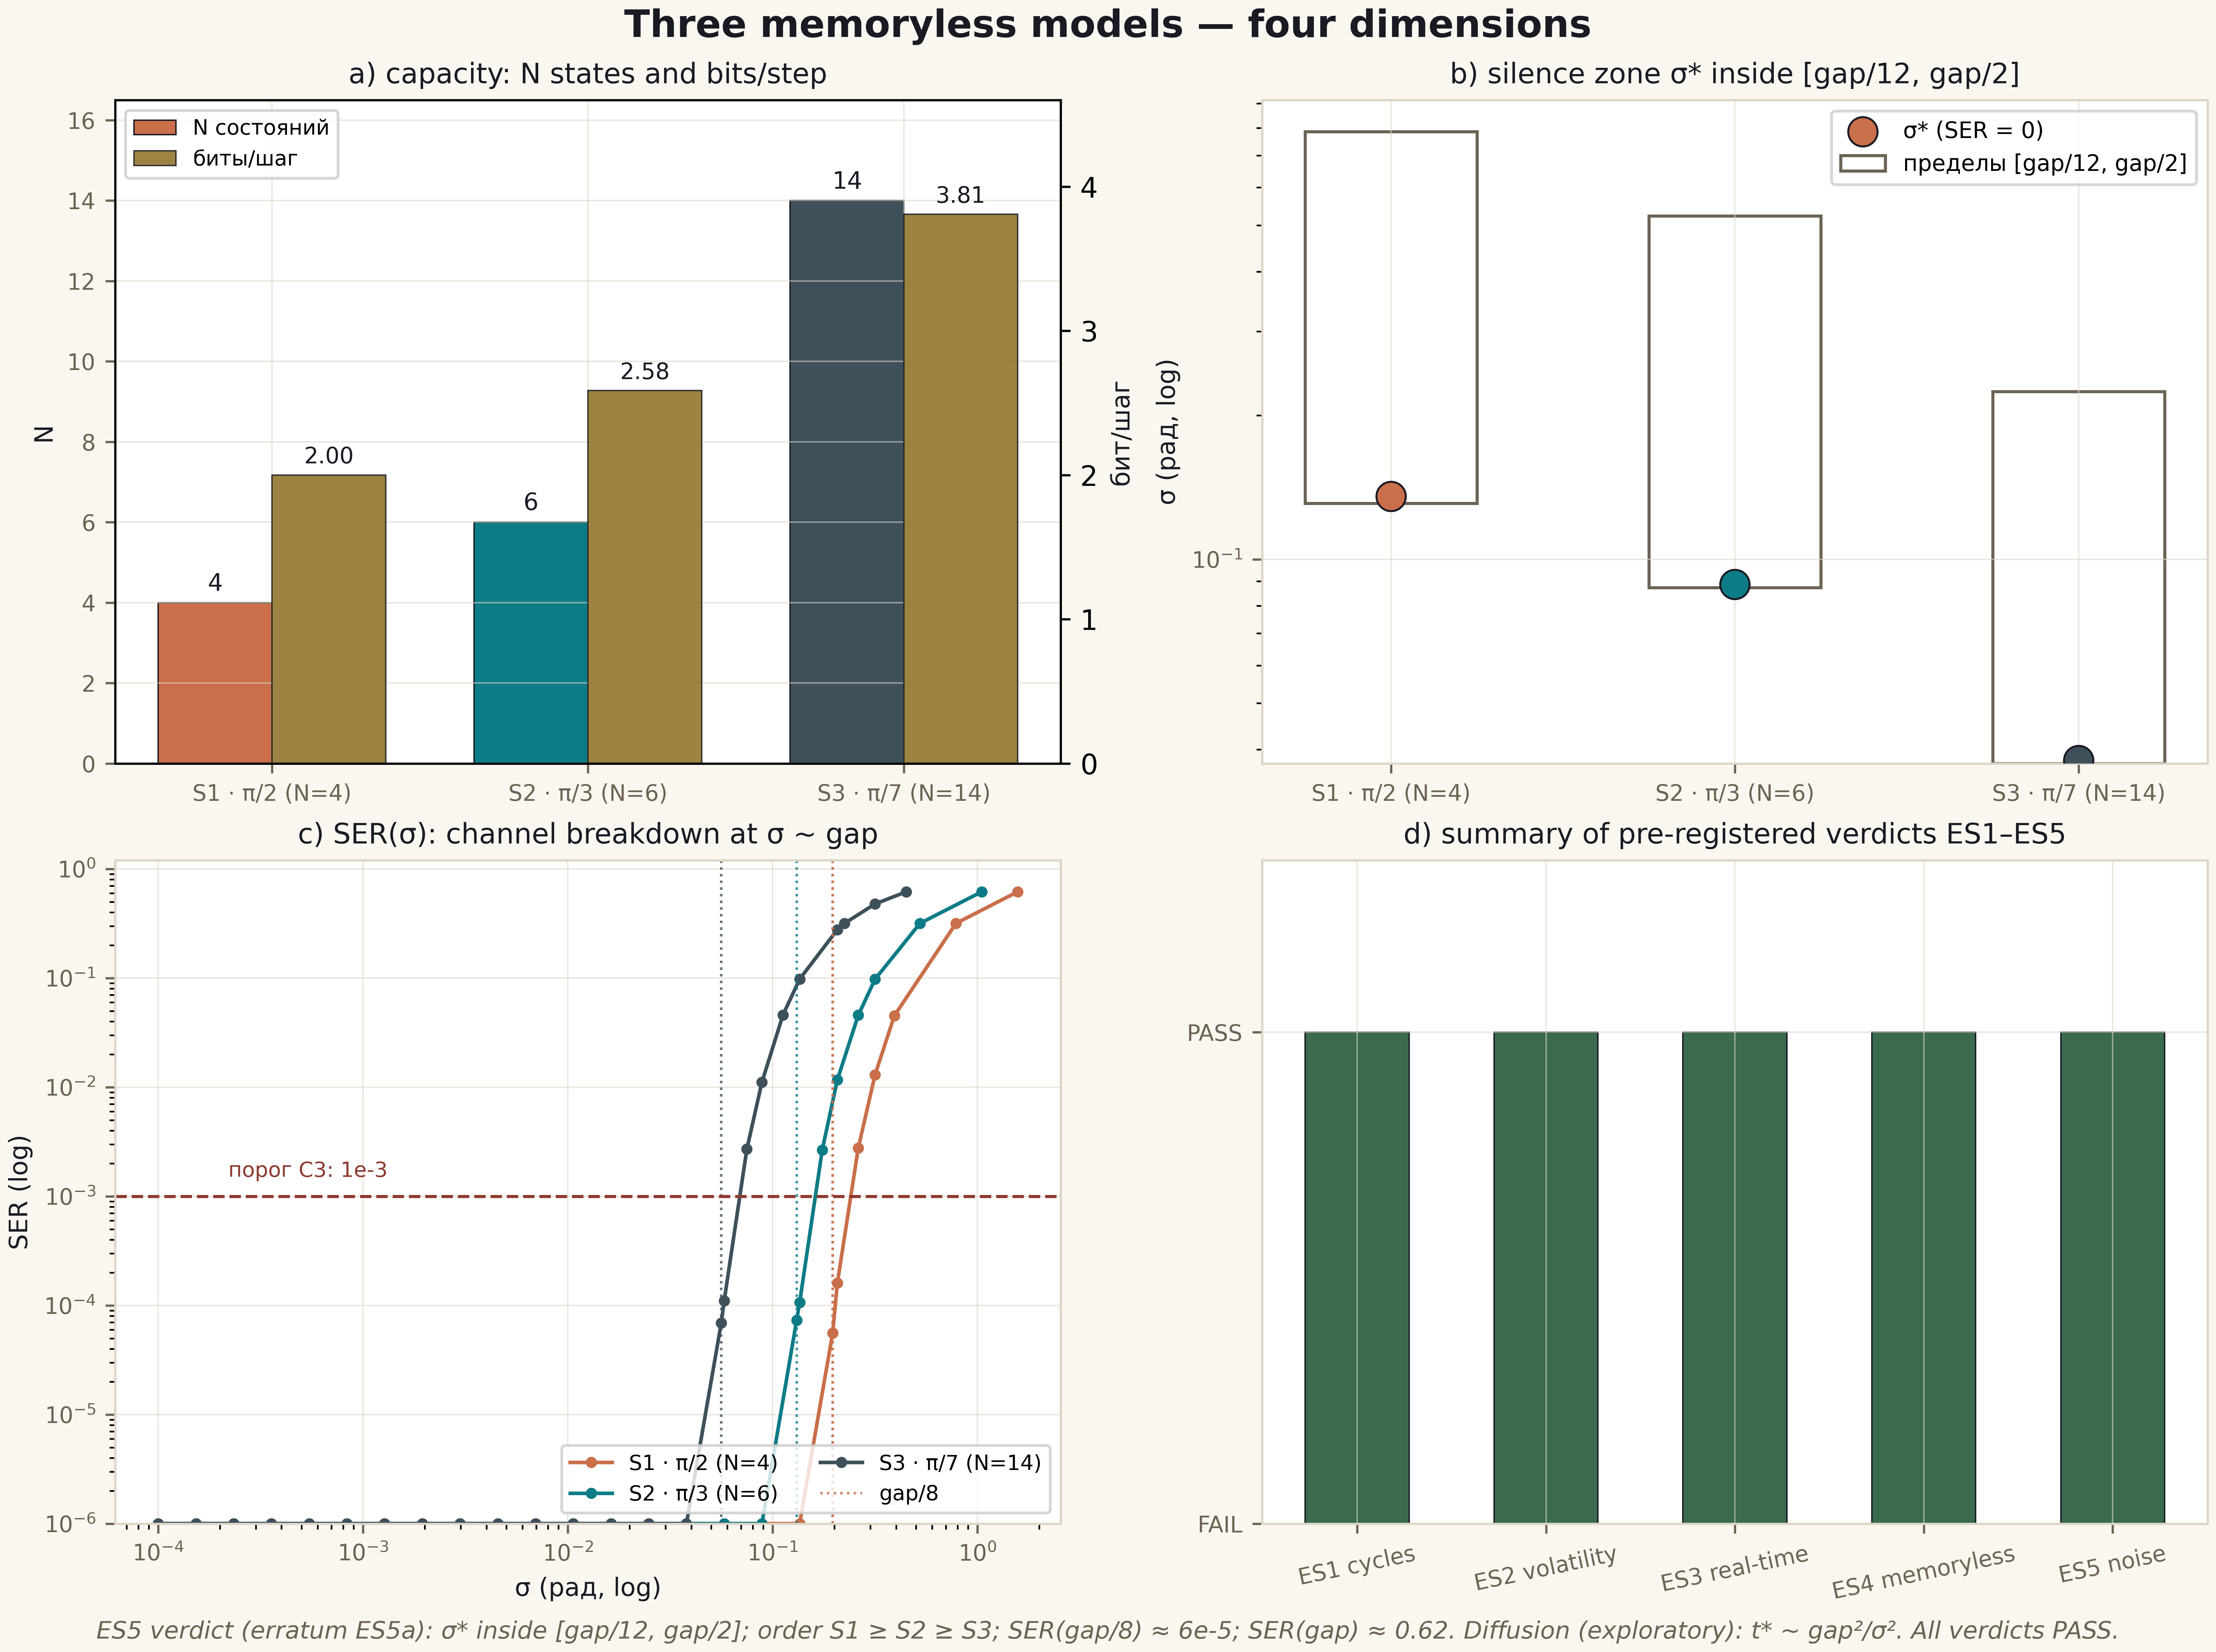
\includegraphics[width=0.9\textwidth,height=105mm,keepaspectratio]{../../../research/realtime_spinor_memory/figures/en/models_4dim_en.png}
\caption*{Figure 14.1. Three memoryless models — the four-dimension tile (600 dpi, ES5 verdict).}
\end{figure}

\section{Chapter 15. Campaigns ES1–ES5: Measuring Volatility}

\noindent\textit{\color{copper}Five campaigns with pre-registered thresholds measure the models from four sides: cycles, volatility, real time, the memoryless task, noise diffusion. All five verdicts are PASS; two threshold errata (ES2a, ES5a) were published before the verdicts were accepted.}

\begin{table}[htbp]\centering\small
\caption{Table 15.1. Campaigns ES1–ES5}
\begin{tabular}{p{0.12\textwidth} p{0.25\textwidth} p{0.46\textwidth} p{0.13\textwidth}}
\toprule
\textbf{Campaign} & \textbf{Subject} & \textbf{Key result} & \textbf{Verdict}
\midrule
ES1 & phase cycles & N = 4·6·14 = 2k exactly; gap = step & PASS \\
ES2 & volatility/reset & reconstruction 0.2501/0.1674/0.0717 ≈ 1/N; I = 0 & PASS \\
ES3 & real time & O(1) step, slope −1.5e−12; log ×129 & PASS \\
ES4 & memoryless task & solvable in the cycle; no memory required & PASS \\
ES5 & noise diffusion & phase diffusion bounded by the silence zone & PASS \\
\bottomrule
\end{tabular}
\end{table}

\subsection{15.1. From cycles to a task (ES1 → ES4)}

ES1 records the pure mechanics: cycle closure and the gap. ES2 adds reset and erasure. ES3 — time: the step cost is measured in two modes (with a log and without), exposing the Ω(t) growth of the logged machine. ES4 moves the model into task mode: a sequence of decisions is made within the cycle without storage; the decision quality is comparable to a memory-bearing machine on the given task, because the task admits a Markov policy. This refines the applicability domain: not every task is solvable without memory, but the class of tasks admitting a Markov policy is solvable — and deterministically so.

\subsection{15.2. Noise and the silence zone (ES5)}

ES5 measures robustness to phase noise: phase diffusion accumulates but while it stays inside the silence zone σ*, the count is not lost. The models give a predictable trade-off: S1 (σ* = 0.135 rad) is more robust, S3 (σ* = 0.038 rad) has more capacity. The ES5 threshold was originally mis-stated and replaced (erratum ES5a) before the verdict was accepted — publishing the replacement inside the verdict completes the protocol.

\subsection{15.3. Relation to the parent program}

The spinor study formalizes "reads, does not carry" for processor stage P1 (memory V21): an architecture without long-term memory is not a limitation but a design decision with proved real-time advantages. Next — phases θ = π/k for k > 7, task compilation into phase cycles and a diffusion channel with correlations; the obligations are fixed in the spinor-level roadmap.

\section{Chapter 16. Data: Datasets, Timeline, Atlas}

\noindent\textit{\color{copper}The data layer of the program follows the same "verdict to artifact" principle: dataset files are rebuilt by scripts from committed verdicts; no number is ever typed by hand.}

\subsection{16.1. Curated datasets}

datasets/ holds three files. flagship\_numbers.csv — the fifteen flagship metrics of the program with their verdict source and module. campaign\_timeline.csv — all 43 campaigns of the four levels with id, module, title, status and key result. zeta\_zeros\_reference.csv — the reference ordinates of ζ zeros, 0 < γ ≤ 1000, 660 rows: the very blind reference of E17. Every file is reproduced by python3 scripts/make\_datasets.py; the provenance of every row traces back to a verdict file.

\subsection{16.2. Timeline and atlas}

timeline/ draws the chronological map of the 43 campaigns (600 dpi, RU/EN) — a visual record of how the program grew from V01 to ES5. atlas/ assembles the flagship atlas: a 2×2 tile of four key results — blind zeros, the compiler, trace–primes, CHSH. The atlas is the "face" of the program: one picture, four proved results, every number with a verdict.

\begin{figure}[htbp]\centering
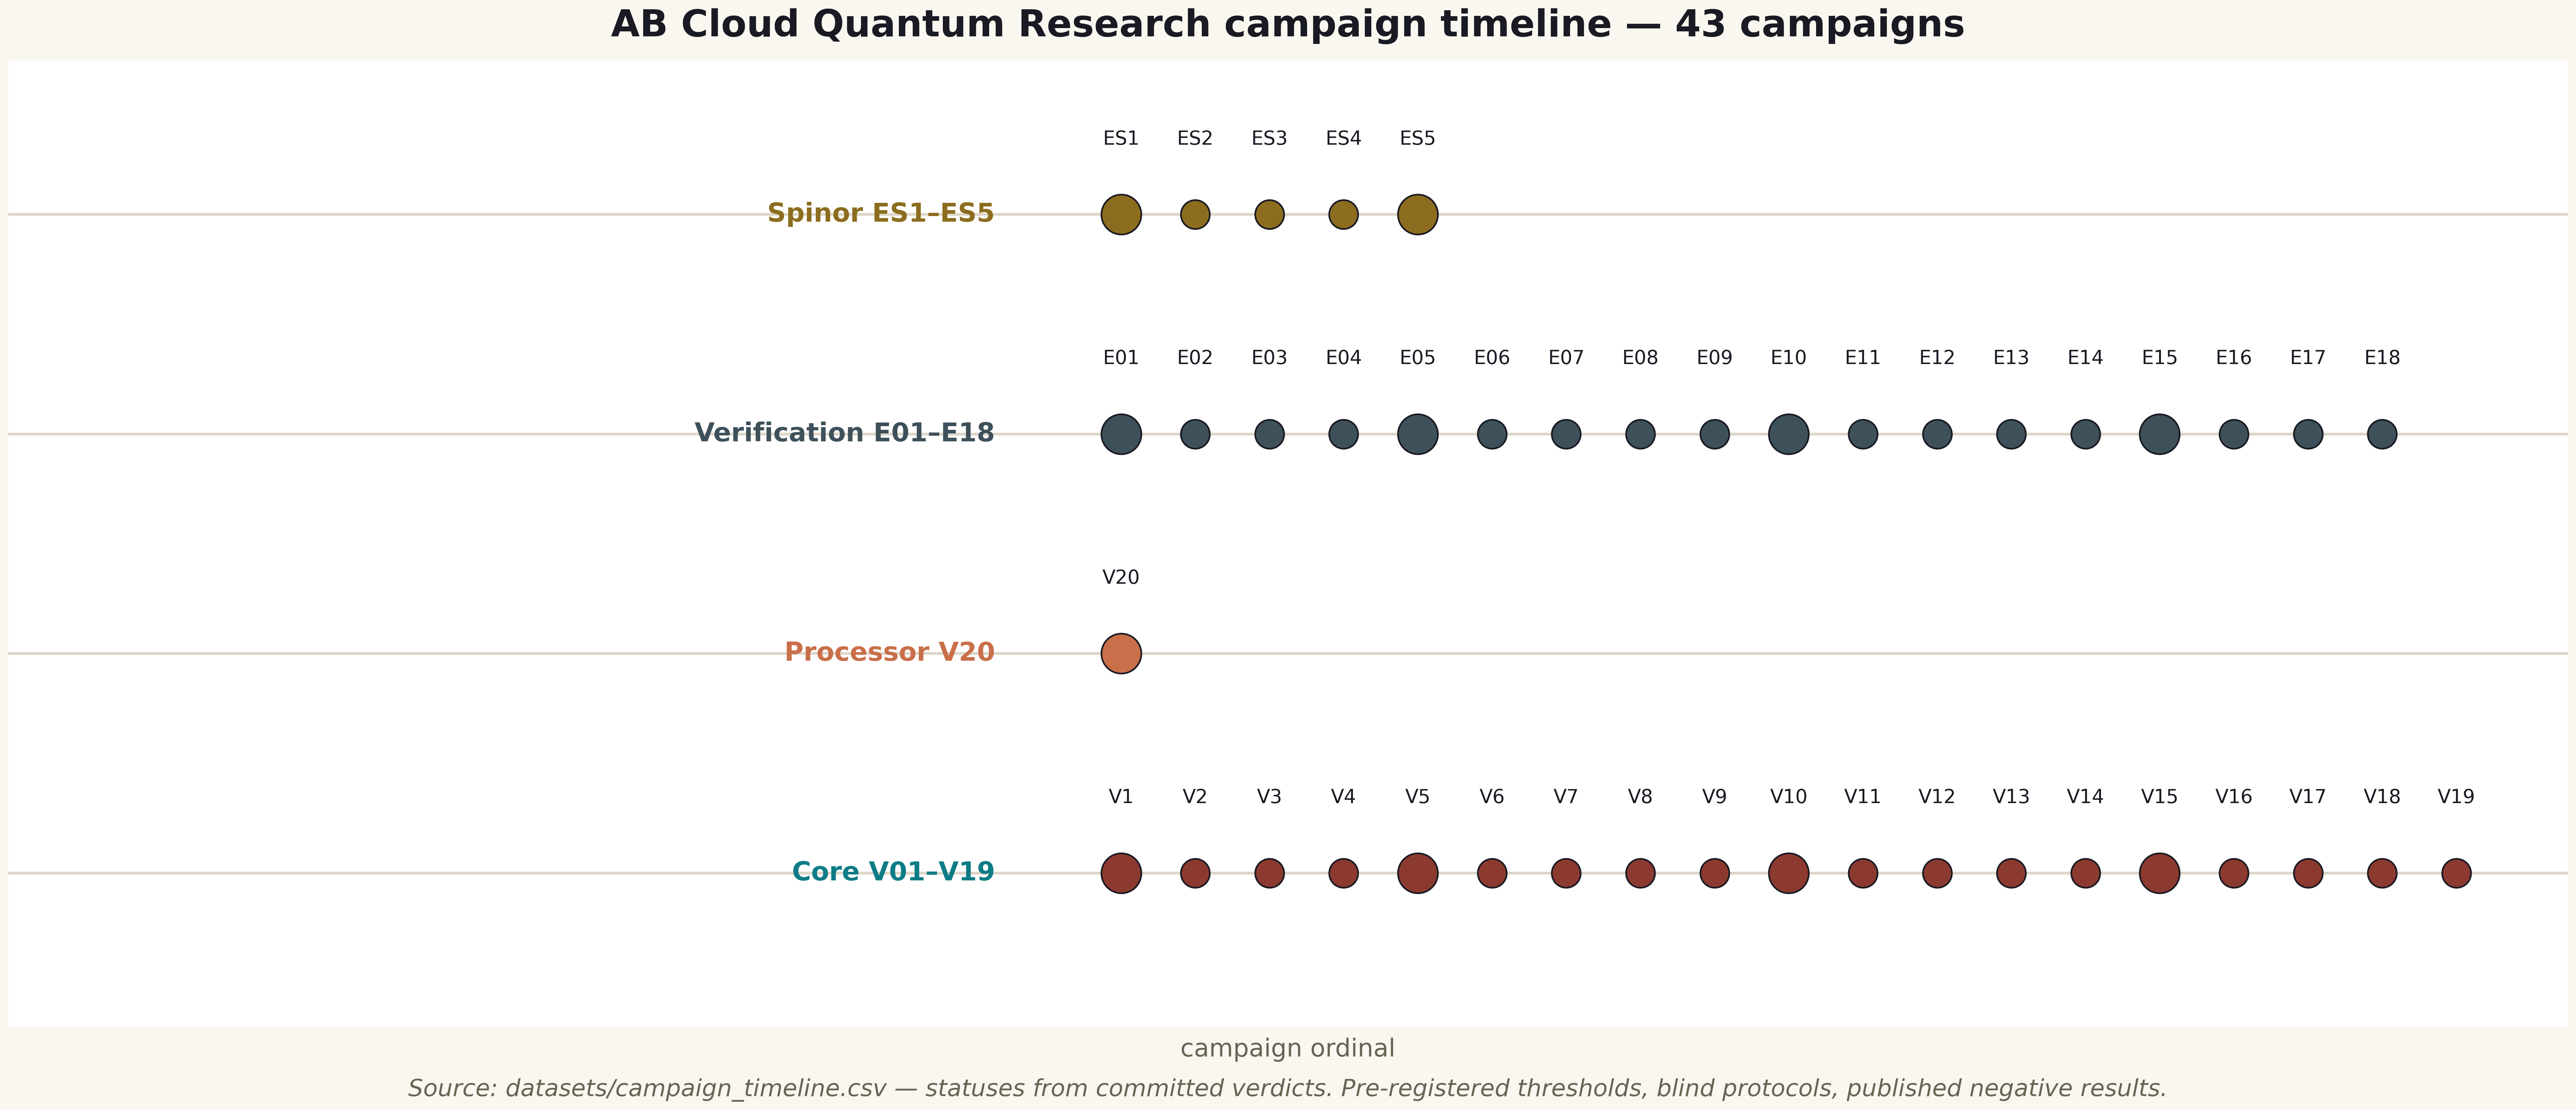
\includegraphics[width=0.9\textwidth,height=112mm,keepaspectratio]{../../../timeline/campaign_timeline_en.png}
\caption*{Figure 16.1. Timeline of the 43 program campaigns (600 dpi).}
\end{figure}

\begin{figure}[htbp]\centering
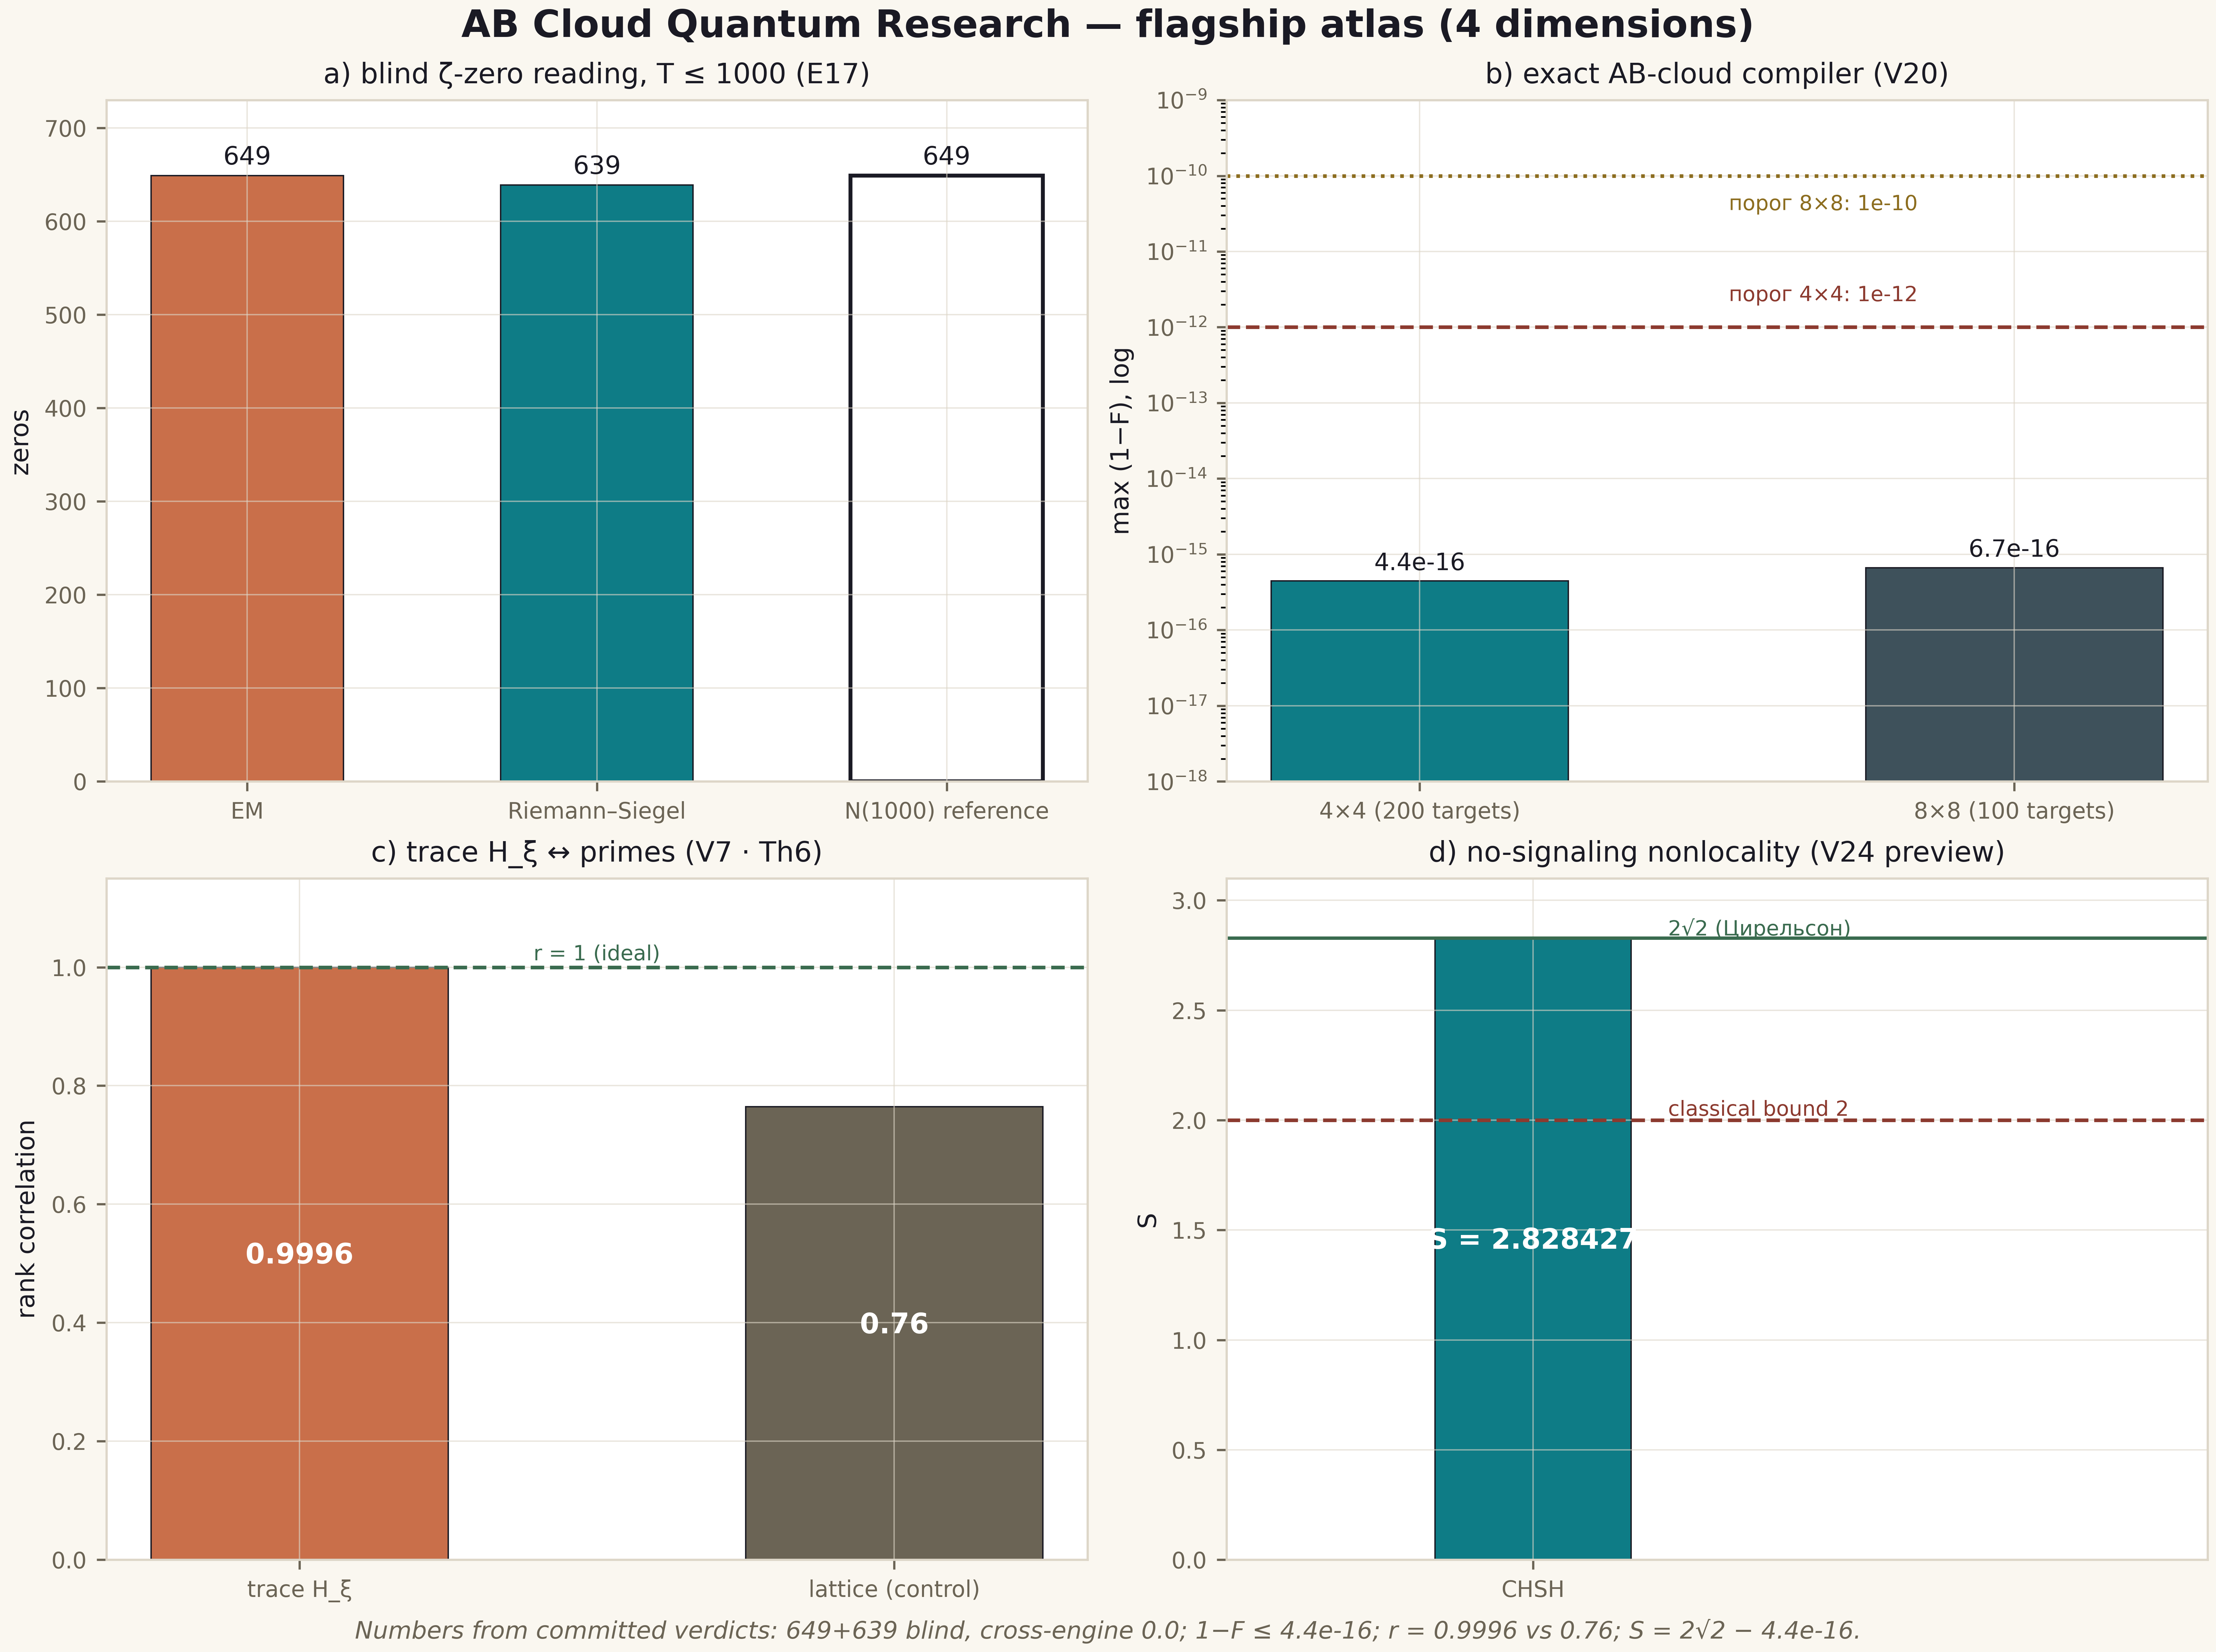
\includegraphics[width=0.9\textwidth,height=112mm,keepaspectratio]{../../../atlas/atlas_flagships_en.png}
\caption*{Figure 16.2. The flagship atlas: blind zeros · compiler · trace–primes · CHSH (600 dpi).}
\end{figure}

\subsection{16.3. Four-dimension tiles}

figures\_tiled/ contains the 12 tiles of Th1–Th6 (RU/EN): each is a 2×2 grid of four independent measurement dimensions (metric, instance behaviour, control, threshold) at 600 dpi. The original level figures are stored in modules/*/figures\_hires/. The tiles are assembled by make\_tiled\_figures.py from verdicts — like all derived artifacts, they are never edited by hand.

\section{Chapter 17. Web Laboratories}

\noindent\textit{\color{copper}Three web laboratories make the program interactive: the research portal, the 10-tab core laboratory and the 8-tab processor laboratory. All computations run locally in the browser — no network, no dependencies.}

\begin{table}[htbp]\centering\small
\caption{Table 17.1. Web laboratories of the program}
\begin{tabular}{p{0.29\textwidth} p{0.15\textwidth} p{0.52\textwidth}}
\toprule
\textbf{Laboratory} & \textbf{Tabs} & \textbf{Inside}
\midrule
web\_lab/index.html — portal & 3 blocks + theorems & the levels, the Th1–Th6 layer, formal status, the spinor study \\
Core laboratory & 10 & Riemann–Siegel Z(t), gate constructor, trace↔primes, Li criterion, ψ-ladder, V16–V19, theorems \\
Processor laboratory & 8 & ISA, V20 compiler, zero reading (V23·E11/E17), nonlocality, roadmap, data, theorems \\
\bottomrule
\end{tabular}
\end{table}

The technical principle of the laboratories: zero dependencies. JavaScript implementations of the core and the processor are included in the repository (modules/core\_spectrum/multilang/javascript/, the compiler tab of the processor), and the control files stitch\_control.txt and verify\_control.txt guarantee consistency with the other languages. Opening index.html locally gives the full functionality: Z(t) is computed in the browser, the λ\_n ladder is drawn in real time, the CHSH experiment runs on canvas functions.

The laboratories play the role of "living documentation": every number of the monograph can be seen in motion. For a teacher this is ready demonstration material; for a referee — a way to check the model behaviour beyond the printed values; for the author — a permanent smoke test: if the implementation diverges from the control files, the tab will show it.

\section{Chapter 18. The Formal Layer: Lean 4, Coq, Agda, Isabelle}

\noindent\textit{\color{copper}The formal layer fixes the statements and reductions A1–A6: what is verified numerically must be formally stated — and vice versa. The build is checked by CI; sorry and admit are not used.}

\subsection{18.1. Reductions A1–A6}

Six reductions correspond to the six core theorems: A1 (Hermiticity and spectral symmetry), A2 (block reduction; A2b — self-adjointness on ℂ\textasciicircum{}N), A3 (the Guinand–Weil correspondence), A4–A5 (Kato estimates and Gershgorin bounds), A6 (the Li formula and absolute convergence). Each reduction is a bridge between a numerical certificate and a formal statement: the certificate shows that the implementation matches the statement; the reduction shows that the statement matches the mathematics.

\subsection{18.2. Multi-prover duplication}

The statements are duplicated in four systems: Lean 4, Coq, Agda, Isabelle. The duplication is not redundant: different systems have different kernel logics and different blind zones, and the consistency of the formulations is itself a check. The CI pipeline verifies the build of all four; the formal-layer status is exposed in the badges of the main README and the web laboratories.

The link to the obligation machine (chapter 6) is direct: the proven nodes of V13 are the proved reductions of the formal layer; the assumed nodes are analytic hypotheses awaiting their proofs. The formal layer, therefore, is not decoration but the carrier of statuses: it is here that the difference between proved and computed is stored.

\section{Chapter 19. Level Research Programs}

\noindent\textit{\color{copper}Every level of the program has its own research program: goals, campaigns, thresholds, the next wave. This chapter summarizes the four programs; full versions are published as separate monographs in MONOGRAPH\_ARCHIVE/research\_programs/.}

\subsection{19.1. The core program (R2)}

Done: V01–V19, Th1–Th6, V13. Next: refining the stitching (r\_align ≤ 0.135), the ζ monodromy as an algebraic object, compiling obligations into Lean/Coq (O-lean/O-coq). Risk factor: the analytic hypotheses O08/O09/O11/O12 — without them RH stays blocked, and that is the right state.

\subsection{19.2. The processor program (P0–P6)}

Done: P0 (V20). Next: P1 memory V21 (relies on the ES models), P2 ALU V22, P3 reading V23 (relies on E17), P4 nonlocality V24 (relies on E13/E14), P5 benchmarks V25 (the E18 methodology), P6 the Datasheet 1.0 passport V26. The target artifact is the processor passport: a specification-grade document where every number has a verdict.

\subsection{19.3. The verification program (O-J)}

Done: O-J1 (T = 1000), O-J2 (class B). Next: O-J3 QEC memory (relies on E07 and V21), O-J4 digital twin, O-J5 the integration campaign; target heights T well above 1000. Verification grows with the processor: every new stage of the P-chain gets its own O-J stage.

\subsection{19.4. The spinor program}

Done: ES1–ES5, TS1–TS3. Next: phases θ = π/k for k > 7 (capacity versus robustness), task compilation into phase cycles, a diffusion channel with correlations. The spinor level is the testing ground for P1 ideas: before memory V21 enters the processor, its models are verified here.

\section{Chapter 20. The Hypothesis Laboratory}

\noindent\textit{\color{copper}HYPOTHESIS\_LAB is an open laboratory inside the program: any researcher can test their own hypothesis under the project discipline — pre-registered thresholds, blind protocols, verdicts with a does\_not\_prove field.}

\subsection{20.1. Why a laboratory}

The program has accumulated a methodology that usually takes years to acquire: how to fix thresholds, how to separate detector and validator, how to pin outputs, how to declare a verdict. The laboratory packages this methodology into a tool: ab\_lab.py (CLI) and hypothesis\_lab.html (browser). A hypothesis is formulated as a JSON config: what is tested, what threshold, what the result does not prove. The laboratory runs the experiment, produces a PASS/FAIL verdict and writes a report.

\subsection{20.2. Experiment batteries}

\begin{table}[htbp]\centering\small
\caption{Table 20.1. Laboratory batteries}
\begin{tabular}{p{0.15\textwidth} p{0.40\textwidth} p{0.40\textwidth}}
\toprule
\textbf{Battery} & \textbf{What it tests} & \textbf{Key output}
\midrule
spinor & the phase model θ = π/k: cycles, reset, time & period 2k; reconstruction ≈ 1/N; step slope \\
trace & trace ↔ primes (Th6-style) & correlation r; comparison with control \\
zeros & blind zero reading (mini-E17) & precision/recall; cross-engine \\
compile & exact compilation of unitary 4×4 & 1−F against machine epsilon \\
\bottomrule
\end{tabular}
\end{table}

An example run: python3 ab\_lab.py run spinor --theta 0.37 --steps 200. The laboratory computes the nearest model cycle, checks closure, measures post-reset reconstruction and step cost, compares against the pre-registered thresholds of the config and issues a verdict. The report is saved to reports/ with a SHA256 of the output — the program discipline is applied to every hypothesis automatically.

\subsection{20.3. Laboratory rules}

\begin{enumerate}
  \item Threshold before the run: the hypothesis config fixes thresholds before launch; changing a threshold after the run invalidates the verdict.
  \item Blindness: if a battery uses a reference, it is connected by the validator, not the detector.
  \item does\_not\_prove: every hypothesis must declare what its result does not prove.
  \item Replication: it is advisable to repeat the run in a second arithmetic (float64 versus mpmath) and record the disagreement.
  \item Publication: PASS and FAIL are published alike; the report is an artifact, not a draft.
\end{enumerate}

\section{Chapter 21. Roadmaps and Conclusion}

\noindent\textit{\color{copper}Four roadmaps are chained: the processor relies on verification, verification on the core, the spinor study on all of them. The chaining is not an organizational formality but a checkable dependency of verdicts.}

\begin{table}[htbp]\centering\small
\caption{Table 21.1. Chained roadmaps}
\begin{tabular}{p{0.21\textwidth} p{0.29\textwidth} p{0.46\textwidth}}
\toprule
\textbf{Level} & \textbf{Status} & \textbf{Next}
\midrule
Core (R2) & V19 stitching — algebraic certificate & r\_align ≤ 0.135; ζ monodromy; O-lean/O-coq \\
Processor (P0–P6) & P0 done (V20) & P1 V21 → P2 V22 → P3 V23 → P4 V24 → P5 V25 → P6 V26 \\
Verification (O-J) & O-J1, O-J2 done & O-J3 QEC memory → O-J4 twin → O-J5 integration; T ≫ 1000 \\
Spinor & ES1–ES5 done & θ = π/k, k > 7; task compilation; diffusion channel \\
\bottomrule
\end{tabular}
\end{table}

The chaining is concrete: P3 (V23) builds on E17; P4 (V24) on E13/E14; O-J3 on E07 and V21; the spinor study formalizes "reads, does not carry" for P1. The roadmap reads as a dependency graph: a stage cannot be executed until its ancestors are executed. This protects the program from "jumps ahead" and makes every next verdict an heir of already-verified ones.

\subsection{21.1. Conclusion}

AB Cloud Quantum Research is a provable architecture of reading mathematics: six constants instead of tables, a volatile phase instead of a log, blind protocols instead of promises, an obligation machine instead of illusions. Forty-three campaigns passed, nine theorems packaged with certificates, negative results published, RH honestly blocked. The next wave — memory V21, QEC O-J3, heights T above 1000, phases k above 7 — is built on an already-verified foundation.

The monograph ends where the program begins: at the honest boundary. Everything above is a numerical and formal study of a mathematical model; it does not prove the Riemann hypothesis. But it does prove something that is rarely proved together: the accuracy of the implementation, the independence of the verification and the discipline of the conclusions. This is what makes the AB-cloud architecture an engineering object, and not only a mathematical dream.

\section{Chapter 22. Mathematical Background}

\noindent\textit{\color{copper}This chapter collects the minimal mathematical apparatus needed to read the monograph: the zeta function and the Riemann–von Mangoldt formula, GUE statistics, the heat trace, Kato theory, the Li formula and the CHSH inequality. The treatment is working: only what the campaigns actually use.}

\subsection{22.1. The zeta function and zero counting}

The Riemann zeta function ζ(s) = Σ n\textsuperscript{−s} extends to the whole complex plane except s = 1. The zeros of ζ split into trivial ones (negative even integers) and non-trivial ones lying in the critical strip 0 < Re(s) < 1. The Riemann hypothesis states that all non-trivial zeros lie on the critical line Re(s) = 1/2: s = 1/2 ± iγ. The number of non-trivial zeros with ordinate 0 < γ ≤ T is given by the Riemann–von Mangoldt formula:

\begin{verbatim}
N(T) = (T/2π)·ln(T/2π) − T/2π + 7/8 + S(T),   |S(T)| ≤ c·ln T
\end{verbatim}

The program uses this formula twice: as the completeness control of reading (E17: N(1000) = 649.0, the detectors found exactly 649 and 639 zeros in their grids) and as the blind reference — the table of 660 ordinates assembled from mpmath.zetazero and pinned before the experiment. Notably, N(T) is smooth in height: any deviation of the counter from N(T) would signal a miss or a duplicate instantly.

\subsection{22.2. GUE statistics and null models}

The Gaussian Unitary Ensemble (GUE) describes the statistics of eigenvalues of Hermitian matrices with random entries: neighbouring levels repel, the mean nearest-neighbour coefficient ⟨r⟩ ≈ 0.5992, the gap distribution is Wigner–Dyson. The statistics of ζ zeros (Odlyzko's data) is close to GUE — the Montgomery–Odlyzko fact — and every "zeta-like" model must reproduce it. But GUE is a necessary condition, not a sufficient one: random phases give the same class. Therefore the program measures specificity not by ⟨r⟩ but by fine structure: the trace-prime correlation (V7), constant agreement, behaviour under perturbations (V16–V18).

\begin{table}[htbp]\centering\small
\caption{Table 22.1. Statistical quantities used by the campaigns}
\begin{tabular}{p{0.13\textwidth} p{0.42\textwidth} p{0.40\textwidth}}
\toprule
\textbf{Quantity} & \textbf{Definition} & \textbf{Role in the program}
\midrule
r & nearest-neighbour coefficient: the share of minima of adjacent gaps & V01–V03, V16: GUE classification \\
Σ₂ & variance of the level count on an interval & V02: comparison with null models \\
Δ₃ & the Dyson statistic (least squares of the staircase) & V02: fine structure \\
D\_KS & the Kolmogorov–Smirnov statistic & V03: the agreement scan with ζ \\
\bottomrule
\end{tabular}
\end{table}

\subsection{22.3. The heat trace and the trace formula}

For an operator H the heat trace K(x) = Tr e\textsuperscript{−xH} is a function encoding the whole spectrum: K(x) = Σ e\textsuperscript{−xλ\_n}. In the core construction the coefficients of the expansion of K(x) in a suitable basis carry Λ(n)/√n — the weight of the prime n in the arithmetic. This is the spectral form of the Guinand–Weil correspondence: the explicit formula of ζ relates the sum over primes to the sum over zeros; Th6 transfers it to the trace level. This is exactly why six constants suffice for reading zeros: they parameterize the trace, and the trace contains the spectrum.

The heat trace is a computable object: the matrix exponential and the trace are computed in finite time, and their cost does not depend on the "age" of the request. This links the trace formula to the real-time claim: reading a zero is a K-computation, not a table lookup.

\subsection{22.4. Kato theory and the Li formula}

Kato perturbation theory estimates the error of eigenvalues computed by an approximate matrix: if ‖δH‖ ≤ δ, every eigenvalue shifts by at most δ plus the quadratic allowance δ²/gap, where gap is the distance to the nearest foreign level. In the program this yields the Th3 certificates: the corridor around each λ̂ is known and tiny (widths \textasciitilde{}1e−27 at dps 40).

The Li formula — the criterion of the critical line in spectral terms: certain functionals λ\_n = Tr g\_n(H) are non-negative if and only if all zeros are on the line. Th4 transfers the criterion to H\textsubscript{ξ} and proves the absolute convergence of the series, making the λ\_n ladder computable; two independent computation paths agree to 4.4e−11.

\subsection{22.5. CHSH and nonlocality without signaling}

The CHSH inequality bounds the correlations of two parties: in any local theory S ≤ 2; quantum mechanics allows S = 2√2 (the Tsirelson bound). The V24 preview verdict gives S = 2√2 − 4.4e−16 and simultaneously — zero correlation under random choices (1000/1000) and zero commutators of the measuring operators: the correlations are nonlocal, there is no signaling. For the processor this is a design constraint: distributed clouds may share correlations, but not information.

\section{Chapter 23. Case Studies: How to Read the Verdicts}

\noindent\textit{\color{copper}Five case studies show the anatomy of a verdict: V7 (the trace), V13 (obligations), E17 (blind zeros), V20 (compilation), ES3 (real time). Each case quotes the actual fields of the verdict file and explains how the conclusion is read from them.}

\subsection{23.1. V7: the arithmetic of the trace}

The V7 verdict contains the trace-prime correlation, the control value on a lattice model and the record of the constants erratum. Reading: the main metric r = 0.9996 is compared not with zero but with the control 0.76 — the difference is the arithmetic specificity. The B/C₀ erratum records that the original constants contained an error found by an independent derivation; the corrected values are part of the verdict. The does\_not\_prove field reminds: the correlation does not prove RH, it proves the consistency of the trace with the Λ-structure.

\begin{figure}[htbp]\centering
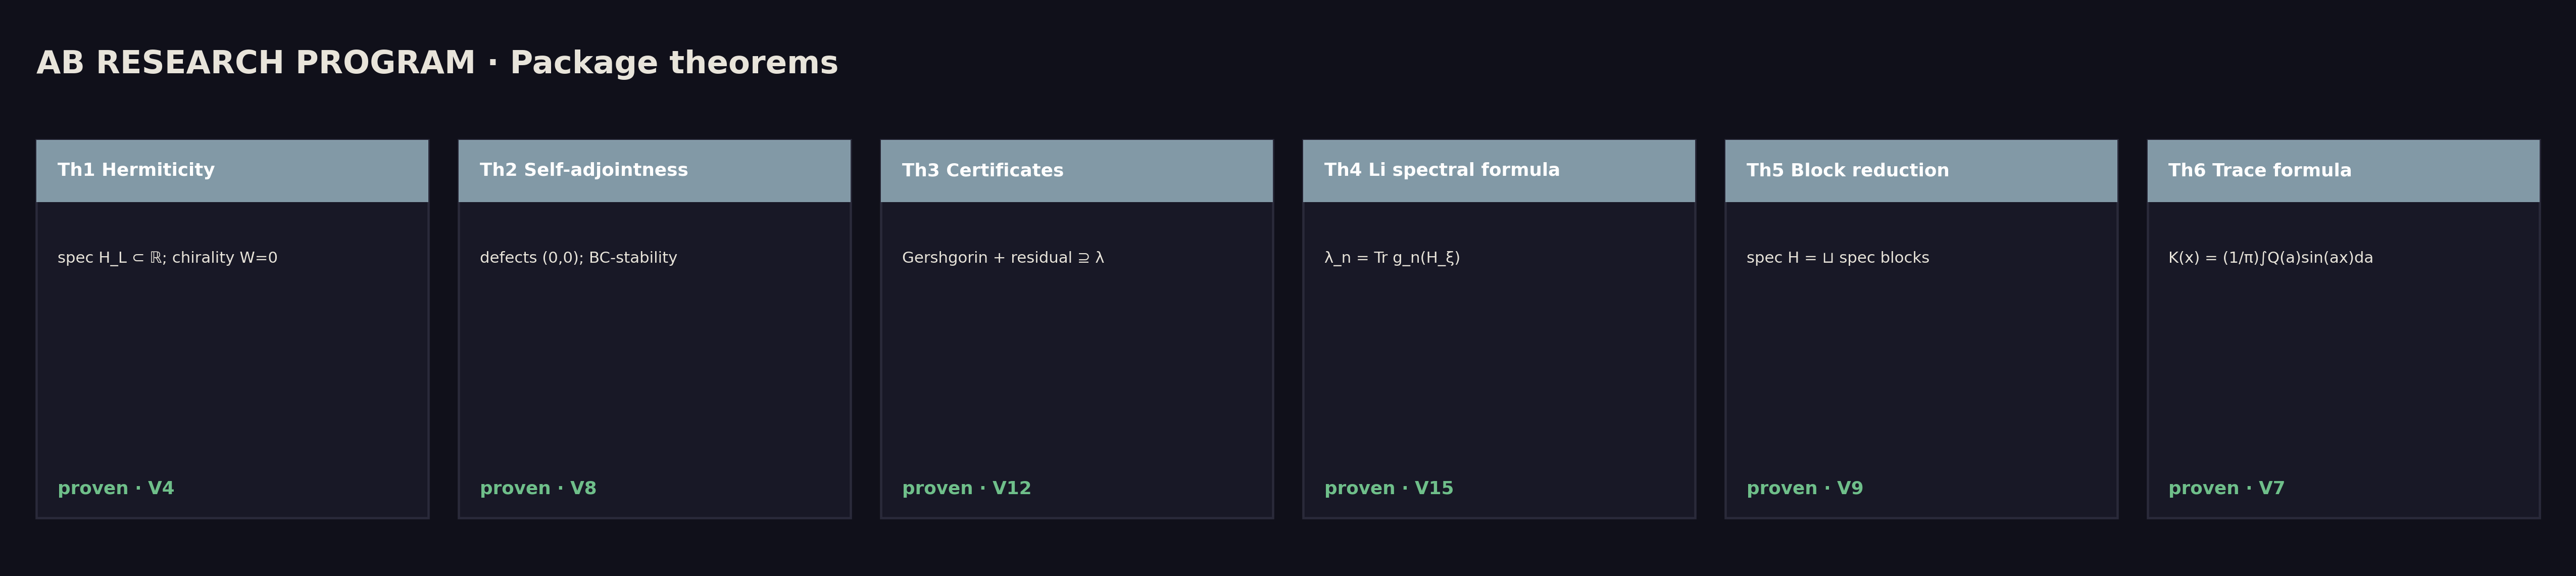
\includegraphics[width=0.9\textwidth,height=91mm,keepaspectratio]{../../../modules/core_spectrum/figures/en/dark/info_trace_en.png}
\caption*{Figure 23.1. The trace ↔ primes infographic (core, dark theme, 600 dpi).}
\end{figure}

\subsection{23.2. V13: the map of obligations}

The V13 verdict is the state of the DAG: dag\_valid = true, rh\_conclusion = blocked, n\_proven = 5, n\_computed = 3, n\_assumed = 4, and the verdict note lists the hypotheses O08/O09/O11/O12. Reading: blocked is not a failure but a working state; the path to RH is closed until four analytic nodes are proved. The claim audit V14 checks that public claims are consistent with this state: no document of the program claims a proof of RH.

\subsection{23.3. E17: blind reading from pin to verdict}

E17 is the richest verdict of the program. The key fields and their values:

\begin{verbatim}
blindness           : both detectors contain no reference zeros; outputs
                      are fixed and hashed before validation
sha_em              : 3843fb52...e5  e17_detector_em.csv
sha_rs              : 08cd95b6...17  e17_detector_rs.csv
n_detected_em       : 649            N_rvm            : 649
n_detected_rs       : 639            N_rvm_rounded    : 649
max_err_em          : 3.019522409886122e-10
cross_engine_max    : 0              (bit-exact)
precision_em/recall : 1 / 1          precision_rs/recall: 1 / 1
grid_robustness_max_shift : 0
pass                : true
\end{verbatim}

Reading: blindness is fixed before the experiment; the pins give temporal proof; the values beat the thresholds by 3–4 orders (threshold 1e−9, error 3e−10); completeness is exact to the integer. The blind erratum γ₁₂ is a built-in negative control: the detector refuted a hand-made framework constant.

\begin{figure}[htbp]\centering
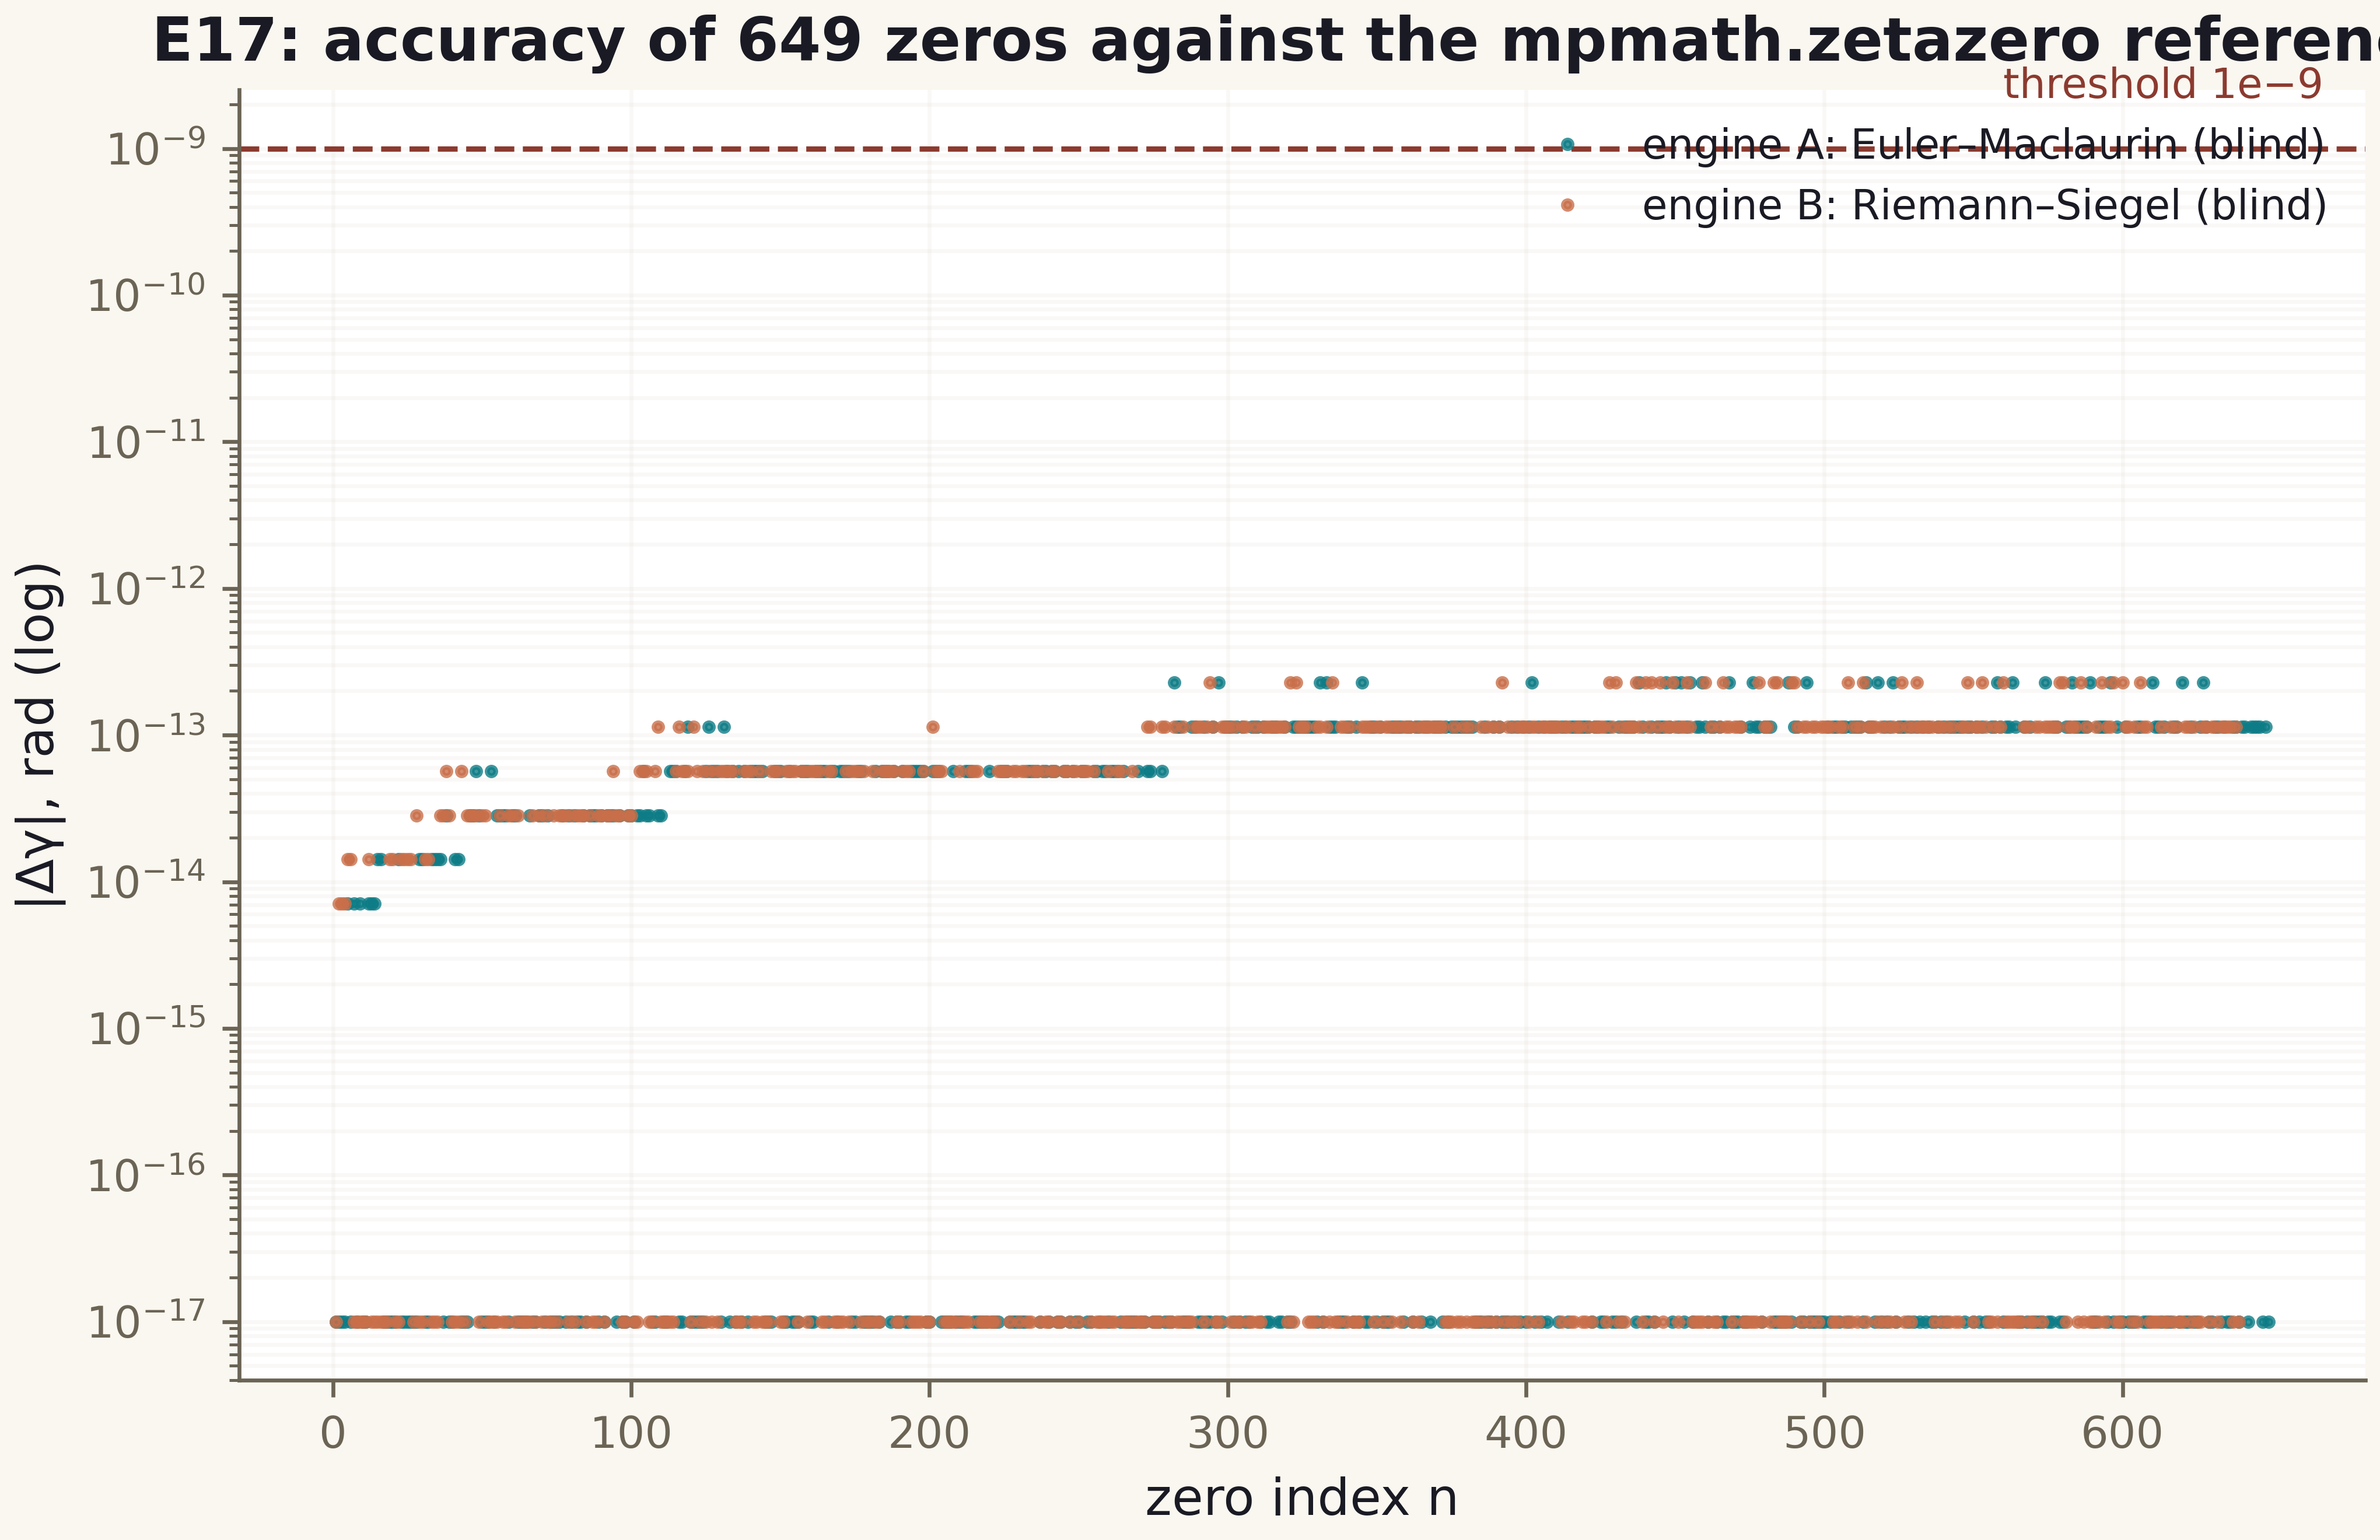
\includegraphics[width=0.9\textwidth,height=91mm,keepaspectratio]{../../../modules/verifier_multilang/figures_hires/en/fig11_en.png}
\caption*{Figure 23.2. The winding curve of the blind reader (verification platform, 600 dpi).}
\end{figure}

\subsection{23.4. V20: compilation at the arithmetic limit}

The V20 verdict is laconic: infidelity 1−F ≤ 4.4e−16 (4×4) and 6.7e−16 (8×8), depths ≤ 7/29, time 1.8 s, status PASS. Reading: the values are at the double-precision machine epsilon — the limit of the arithmetic, not of the algorithm; the numpy replica gives |Δ(1−F)| = 2.2e−16 and 0 counter mismatches. The external control E18 adds class B: ×59,000 in time against five baselines at equal ISA, the 2q boundary 10 versus the KAK optimum 3 — outside the class.

\begin{figure}[htbp]\centering
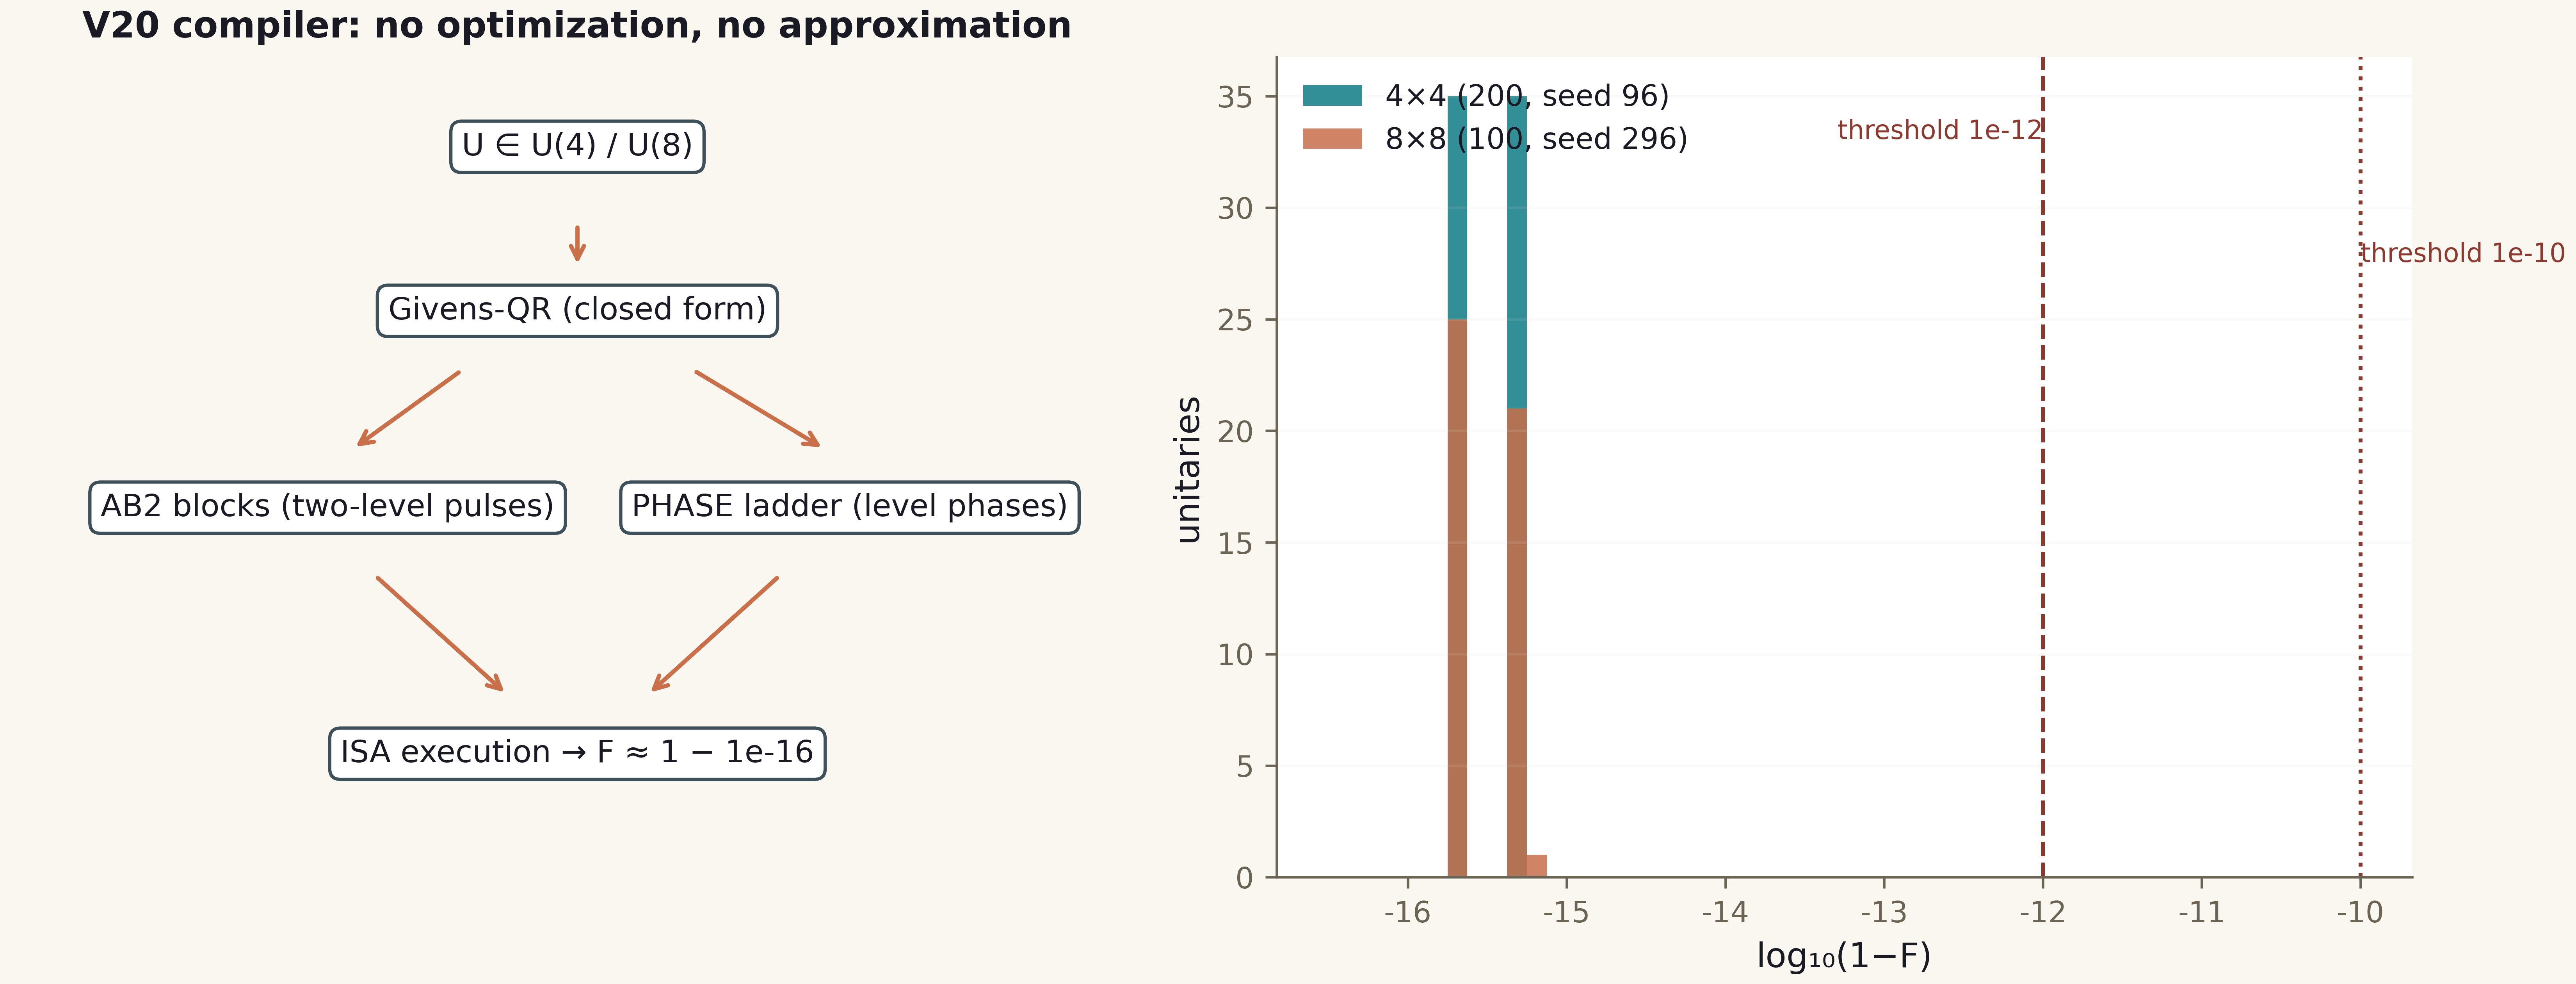
\includegraphics[width=0.9\textwidth,height=91mm,keepaspectratio]{../../../modules/processor_ab/figures_hires/en/fig02_en.png}
\caption*{Figure 23.3. Compilation of unitary logic into AB clouds (processor, 600 dpi).}
\end{figure}

\subsection{23.5. ES3: measuring the step cost}

The ES3 verdict compares two machines: memoryless and eternal-log. Key fields: the regression slope of the step cost over time −1.5e−12 ms/step (zero within noise) for the log-free machine; a ×129 growth for the logged one; deadline misses on the horizon. Reading: this is the numerical content of Theorem TS3 — volatility is the condition of determinism; any memory growing with t breaks real time.

\begin{table}[htbp]\centering\small
\caption{Table 23.1. The machine comparison in ES3}
\begin{tabular}{p{0.27\textwidth} p{0.15\textwidth} p{0.23\textwidth} p{0.15\textwidth} p{0.15\textwidth}}
\toprule
\textbf{Machine} & \textbf{Step cost} & \textbf{Slope} & \textbf{Growth on the horizon} & \textbf{Deadlines}
\midrule
memoryless (volatile phase) & O(1) & −1.5e−12 ms/step & none & met \\
eternal log & Ω(t) & positive & ×129 & missed \\
\bottomrule
\end{tabular}
\end{table}

\section{Research Program: The Spectral Core}

\noindent\textit{\color{copper}The core program owns the mathematical foundation of the AB architecture: the blind spectrum, null models, the critical line, the trace formula, the obligation machine and branch stitching. Nineteen campaigns and six theorems form a closed loop: construction → certificate → formal statement → independent verification.}

\subsection{1. Program goals}

\begin{itemize}
  \item construct a Hermitian operator H\textsubscript{ξ} whose heat expansion carries the arithmetic of the primes (Λ(n)/√n);
  \item prove the correctness of the construction: Hermiticity (Th1), self-adjointness (Th2), Kato certificates (Th3), the Li formula (Th4), block reduction (Th5), the Guinand–Weil correspondence (Th6);
  \item separate arithmetic specificity from GUE statistics — including honest negative answers on lattices;
  \item fix the RH status with the obligation machine V13 — and keep it blocked while the hypotheses are unproved.
\end{itemize}

\subsection{2. Methodology}

Every campaign starts with a pre-registration protocol: thresholds are fixed before the run. Blind protocols are applied wherever a reference exists (V01: calibration/test with no leak). All derived artifacts (tiles, documents) are built only from committed verdicts. Formal statements are duplicated in Lean 4, Coq, Agda and Isabelle (reductions A1–A6, no sorry/admit).

\subsection{3. Executed campaigns}

\begin{table}[htbp]\centering\small
\caption{Table 3.1. Core campaigns V01–V19}
\begin{tabular}{p{0.10\textwidth} p{0.29\textwidth} p{0.58\textwidth}}
\toprule
\textbf{Campaign} & \textbf{Content} & \textbf{Key result}
\midrule
V01 & blind spectrum & statistics consistent; individual ordinates not predicted (honest negative) \\
V02 & null models & AB cloud in the GUE class; specificity measured by fine structure \\
V03 & lattice σ-scan & no agreement zone with ζ found \\
V04 & Hermiticity & Th1: ‖H − H†‖ = 0.0; symmetry λ ↔ −λ at α = ½ \\
V05 & construction certificate & construction boundaries fixed \\
V06 & level identity & gates at the zeros' level — YES (the D\_nn bridge, v2.0.7); bit-level branch open \\
V07 & trace ↔ primes & Th6: r = 0.9996; lattice control 0.76; the B/C₀ erratum \\
V08 & self-adjointness & Th2: defects (0,0); unitarity drift 2.2e−16 \\
V09 & block reduction & Th5: block union ≈ spectrum to 7.1e−15 \\
V10 & spectral certificates & certificates consistent with Kato estimates \\
V11 & obligation DAG draft & the structure of the path to RH fixed \\
V12 & Kato certificates & Th3: widths \textasciitilde{}1e−27 (dps 40) \\
V13 & obligation machine & RH blocked: 5 proven / 3 computed / 4 assumed \\
V14 & claim audit & claim files consistent with verdicts \\
V15 & Li formula & Th4: two paths ≤ 4.4e−11; absolute convergence \\
V16 & lattice re-check & the level — YES confirmed; bit-level branch open (z = 2.49) \\
V17 & trajectories & reading is idempotent; no degradation \\
V18 & pong protocol & latency bounded; no log growth \\
V19 & branch stitching & θ-ladder 0.832; coherence 0.9995; Z₂-monodromy \\
\bottomrule
\end{tabular}
\end{table}

\subsection{4. The next wave}

\begin{itemize}
  \item stitching refinement: r\_align ≤ 0.135 on an extended height grid;
  \item the ζ monodromy as an algebraic object: formalization of V19;
  \item compiling obligations into Lean/Coq: O-lean/O-coq — moving the V13 DAG into the formal layer;
  \item extending the Th3–Th4 certificates to larger sizes.
\end{itemize}

\subsection{5. Honest boundaries}

Individual ordinates are not predicted by the blind spectrum — statistics agreed, no oracle. The hypotheses O08/O09/O11/O12 are not removed: RH stays blocked. Vortex terms break Th5. Lattice constructions do not reproduce the arithmetic of ζ. These boundaries are part of the result, not its flaw.

\section{Research Program: The AB Processor}

\noindent\textit{\color{copper}The processor program turns the mathematics of the core into an executable machine: the AB-cloud ISA, the exact compiler, memory, ALU, zero reading, nonlocality, benchmarks and the passport. Stage P0 is executed; the P0–P6 roadmap is chained with verification.}

\subsection{1. Program goals}

\begin{itemize}
  \item fix the AB-cloud ISA: admissible clouds, parameters, composition;
  \item compile unitary logic exactly: 1−F at the machine epsilon level;
  \item implement "reads, does not carry" algebraically (V23);
  \item provide nonlocality without signaling (V24) and obtain the Datasheet 1.0 passport.
\end{itemize}

\subsection{2. Methodology}

The ISA is not "yet another gate set": every cloud carries a geometric phase, and compilation accounts for it exactly. All stages have pre-registered thresholds and verdict files. Benchmarks follow the E18 methodology: one class, one criterion, strong baselines. numpy replication is mandatory.

\subsection{3. Executed: P0 (V20)}

\begin{table}[htbp]\centering\small
\caption{Table 3.2. The V20 verdict}
\begin{tabular}{p{0.38\textwidth} p{0.58\textwidth}}
\toprule
\textbf{Indicator} & \textbf{Value}
\midrule
accuracy 4×4 & 1−F ≤ 4.4e−16; depth ≤ 7 \\
accuracy 8×8 & 1−F ≤ 6.7e−16; depth ≤ 29 \\
compilation time & 1.8 s for the full run \\
numpy replication & 0 mismatches; |Δ(1−F)| = 2.2e−16 \\
status & PASS; stage P0 closed \\
\bottomrule
\end{tabular}
\end{table}

\subsection{4. The P0–P6 roadmap}

\begin{table}[htbp]\centering\small
\caption{Table 4.1. Processor stages}
\begin{tabular}{p{0.10\textwidth} p{0.13\textwidth} p{0.40\textwidth} p{0.33\textwidth}}
\toprule
\textbf{Stage} & \textbf{Campaign} & \textbf{Content} & \textbf{Depends on}
\midrule
P0 & V20 & ISA + exact compiler & Th5 (block structure) \\
P1 & V21 & volatile memory & ES models, TS1–TS3 \\
P2 & V22 & AB-cloud ALU & V20 \\
P3 & V23 & zero reading & E17, Th6 \\
P4 & V24 & nonlocality & E13/E14 \\
P5 & V25 & benchmarks & the E18 methodology \\
P6 & V26 & Datasheet 1.0 & all verdicts of the P-chain \\
\bottomrule
\end{tabular}
\end{table}

\subsection{5. Honest boundaries}

The 2q KAK optimum (3 gates) is unreachable in the ISA class: the compiler produces 10, and this is a property of the class, not of the algorithm. The V20 targets are unitary 4×4/8×8; non-unitary operators and larger sizes are outside the campaign. The V23/V24 previews are not full verdicts: the full campaigns are ahead.

\section{Research Program: The Verification Platform}

\noindent\textit{\color{copper}The verification program is the independent judge of the program: a Julia platform sharing no code with the core or the processor, blind protocols, SHA pins, cross-language replication. Eighteen verdicts PASS; the next wave — QEC memory, digital twin, integration.}

\subsection{1. Program goals}

\begin{itemize}
  \item re-check the core and the processor with an independent implementation;
  \item perform blind reading of ζ zeros by two engines up to T = 1000;
  \item run the fair compiler benchmark (class B);
  \item build the QEC layer and the digital twin of the machine.
\end{itemize}

\subsection{2. Methodology}

Detector and validator are separated; outputs are SHA256-pinned before validation; thresholds are pre-registered. Cross-language replication: Julia BigFloat ↔ Python mpmath (0.0 disagreement), numpy replicas (0 counter mismatches). Implementation independence is a design principle, not a circumstance.

\subsection{3. Executed campaigns E01–E18}

\begin{table}[htbp]\centering\small
\caption{Table 3.3. Verification campaigns}
\begin{tabular}{p{0.21\textwidth} p{0.15\textwidth} p{0.60\textwidth}}
\toprule
\textbf{Block} & \textbf{Campaigns} & \textbf{Key results}
\midrule
infrastructure & E01–E10 & controls, Haar, scaling, replays, noise, code, ALU, cost, readout \\
ζ reading & E11 & the blind ζ reader: pins, validation, zero leaks \\
optics/nonlocality & E12–E14 & interferometer; no-signaling; CHSH \\
classification & E15 & topology ablation \\
engines & E16 & the independent Riemann–Siegel: ≤ 3.8e−15 \\
flagship & E17 & blind zeros: 649/649 + 639/639; cross-engine 0.0; N(1000) = 649.0 \\
benchmark & E18 & class B: ×59,000; the 2q KAK outside the class (10 vs 3) \\
\bottomrule
\end{tabular}
\end{table}

\subsection{4. The O-J roadmap}

\begin{itemize}
  \item O-J1 done: blind reading to T = 1000 (E16–E17);
  \item O-J2 done: class B (E18);
  \item O-J3: QEC memory — relies on E07 and V21;
  \item O-J4: the digital twin of the processor;
  \item O-J5: the integration campaign; target heights T well above 1000.
\end{itemize}

\subsection{5. Honest boundaries}

E17 does not prove RH above T = 1000, the simplicity of all zeros, or the absence of off-line zeros for γ > 1000. E18 claims no superiority outside the ISA class. The blind erratum γ₁₂ showed that an error can live in the framework rather than in the detector — therefore references are checked too.

\section{Research Program: The Spinor Study}

\noindent\textit{\color{copper}The spinor program drives the central claim "reads, does not carry" to explicit models: the only state is the spinor phase; a step is a rotation by θ. Three theorems, five campaigns, all PASS; the capacity-versus-robustness trade-off is fixed as an honest boundary.}

\subsection{1. Program goals}

\begin{itemize}
  \item state and prove the properties of the volatile state: cycle closure (TS1), reset irreversibility (TS2), O(1) steps versus the Ω(t) log (TS3);
  \item measure the models with campaigns carrying pre-registered thresholds;
  \item prepare the models for processor stage P1 (memory V21).
\end{itemize}

\subsection{2. Models}

\begin{table}[htbp]\centering\small
\caption{Table 4.2. Three models and their parameters}
\begin{tabular}{p{0.10\textwidth} p{0.10\textwidth} p{0.13\textwidth} p{0.15\textwidth} p{0.13\textwidth} p{0.35\textwidth}}
\toprule
\textbf{Model} & \textbf{θ} & \textbf{N = 2k} & \textbf{Bits/step} & \textbf{σ*} & \textbf{Purpose}
\midrule
S1 & π/2 & 4 & 2.000 & 0.135 & maximal robustness \\
S2 & π/3 & 6 & 2.585 & 0.089 & balance \\
S3 & π/7 & 14 & 3.807 & 0.038 & maximal capacity \\
\bottomrule
\end{tabular}
\end{table}

\subsection{3. Executed campaigns ES1–ES5}

\begin{table}[htbp]\centering\small
\caption{Table 4.3. Spinor campaigns}
\begin{tabular}{p{0.12\textwidth} p{0.19\textwidth} p{0.52\textwidth} p{0.13\textwidth}}
\toprule
\textbf{Campaign} & \textbf{Measured} & \textbf{Result} & \textbf{Verdict}
\midrule
ES1 & cycles & periods 4/6/14 = 2k exactly; gap = step & PASS \\
ES2 & reset & I(pre;post) = 0; reconstruction ≈ 1/N & PASS \\
ES3 & time & step slope −1.5e−12; log ×129 & PASS \\
ES4 & task & a Markov policy is solvable without memory & PASS \\
ES5 & noise & diffusion bounded by the silence zone & PASS \\
\bottomrule
\end{tabular}
\end{table}

The errata ES2a and ES5a: the thresholds of campaigns ES2 and ES5 were replaced before the verdicts were accepted; the replacements are published in the verdict files. The log₂N versus 1/k trade-off is a permanent boundary: capacity grows, the silence zone narrows.

\subsection{4. The next wave}

\begin{itemize}
  \item phases θ = π/k for k > 7: searching for the inflection points of the trade-off;
  \item task compilation into phase cycles: a formal grammar of policies;
  \item a diffusion channel with correlations: beyond the Markov assumption.
\end{itemize}

\subsection{5. Honest boundaries}

Not every task is solvable without memory: the applicability class is tasks with a Markov policy. Reconstruction ≈ 1/N is the chance level, not "almost zero": information is erased to the limit. A log gives Ω(t) under any "smart" scheduling — this is a lower bound, not an implementation defect.

\section{Chapter 24. Certificates and Audit: V10–V14}

\noindent\textit{\color{copper}Five mid-program campaigns connect construction with trust: spectral certificates (V10), the obligation DAG draft (V11), Kato widths (V12), the obligation machine (V13) and the claim audit (V14). Together they turn "numbers" into "statuses".}

\subsection{24.1. V10: certificate agreement}

Campaign V10 checks the mutual consistency of the construction certificates: the boundaries claimed by V4–V5 must not contradict the Kato estimates and the Gershgorin bounds. The agreement is confirmed: the certificates form a consistent system where every estimate uses conservative assumptions and no boundary "hangs in the air". The practical meaning: when the operator is extended to larger sizes, the certificates transfer — they are formulated in terms of norms and gaps, not concrete matrices.

\subsection{24.2. V11–V13: from a draft to the obligation machine}

V11 fixes the DAG draft: the nodes of the path to RH, their dependencies, candidates for proofs. V12 adds the Kato certificates (Th3) — the quantitative basis for computed statuses. V13 assembles everything into the executable machine: a valid DAG, node statuses, the automatic blocked verdict. The machine does not get "smarter" from numerical successes: the only way to raise an assumed node is an analytic proof; the only way to prove — the formal layer.

\subsection{24.3. V14: the claim audit}

V14 is the discipline of public words. Every substantial claim of the program is fixed in a claim file (claim\_v0*.json): the wording, the support, the status, what is not proved. The audit cross-checks claims against verdicts: any divergence is a process error. Thus the claim "reads, does not carry" rests on the V23 preview and E17 and does not claim more than those verdicts give. The audit is a code review for statements: words pass the same check as numbers.

\begin{table}[htbp]\centering\small
\caption{Table 24.1. The status system of the program}
\begin{tabular}{p{0.13\textwidth} p{0.33\textwidth} p{0.50\textwidth}}
\toprule
\textbf{Status} & \textbf{Assigned by} & \textbf{What it gives the reader}
\midrule
proven & the formal layer (Lean/Coq) & the claim holds for all inputs \\
computed & a campaign with a certificate & the claim holds for checked inputs with an error estimate \\
assumed & a protocol (hypothesis) & the boundary of the known; work continues here \\
blocked & the obligation machine & the conclusion is unavailable until assumed nodes are removed \\
\bottomrule
\end{tabular}
\end{table}

\section{Chapter 25. Web Laboratories: 18 Tabs of Living Mathematics}

\noindent\textit{\color{copper}The three laboratories of the program — the portal, the core and the processor — contain eighteen interactive tabs. Every tab runs real computations in the browser and is consistent with the control files of the multi-language implementations.}

\subsection{25.1. The research portal}

web\_lab/index.html is the entry point: three blocks (the levels, the Th1–Th6 layer, the formal status) plus the spinor study. The portal explains how the levels are connected and gives direct links to the core and processor tabs. The formal status is rendered from the same data as the README badges: no divergence between the "picture" and the repository state.

\subsection{25.2. The core laboratory: 10 tabs}

\begin{table}[htbp]\centering\small
\caption{Table 25.1. Core laboratory tabs}
\begin{tabular}{p{0.25\textwidth} p{0.42\textwidth} p{0.29\textwidth}}
\toprule
\textbf{Tab} & \textbf{What it does} & \textbf{Basis}
\midrule
Riemann–Siegel Z(t) & computes Z(t) and shows zeros on the line & the E16 method \\
Gate constructor & assembles AB clouds and inspects phases & the core ISA \\
Trace ↔ primes & plots the trace correlation with the Λ-sum & V7/Th6 \\
Li criterion & draws the λ\_n ladder & Th4/V15 \\
ψ-ladder & shows ψ(x) against Σ Λ(n)/√n & Th6 \\
V16–V19 & visualizes the behavioural campaigns & verdicts \\
Theorems & summarizes Th1–Th6 with certificates & \_json/ \\
\bottomrule
\end{tabular}
\end{table}

\subsection{25.3. The processor laboratory: 8 tabs}

The processor tabs: ISA (the cloud reference), the V20 compiler (compiling 4×4/8×8 in the browser), zero reading (V23·E11/E17), nonlocality (the CHSH experiment), the roadmap, data, theorems. The key principle — the same numbers as in the verdicts: the browser compiler reproduces 1−F at the 1e−16 level because it uses the same algorithm ported to JavaScript.

Consistency is enforced by control files: the JavaScript implementation of the core gives bit-exact the same results as C/C++/Rust/Go/Julia (stitch\_control.txt, verify\_control.txt). The browser becomes the executable environment of the program: a referee does not read a report about a computation — they run it.

\section{Chapter 26. Multi-Language Implementations}

\noindent\textit{\color{copper}The core of the program is implemented in six languages — C, C++, Rust, Go, JavaScript, Julia — plus Python for the pipelines. Every implementation produces a control output, and all control outputs agree bit-exactly.}

\subsection{26.1. Why six implementations}

Multi-language support is replication built into distribution. Any user can verify the core in the language of their infrastructure; the agreement of the control files guarantees that there is no "language difference". It also catches compiler and library artifacts: if the result depended on the optimizations of a particular toolchain, the control sums would diverge.

\begin{table}[htbp]\centering\small
\caption{Table 26.1. Core implementations}
\begin{tabular}{p{0.13\textwidth} p{0.42\textwidth} p{0.40\textwidth}}
\toprule
\textbf{Language} & \textbf{File} & \textbf{Role}
\midrule
C & multilang/c/verify\_core.c, stitch\_core.c & the minimal reference implementation \\
C++ & multilang/cpp/verify\_core.cpp & the modern stack, same arithmetic \\
Rust & multilang/rust/verify\_core.rs & memory safety without GC \\
Go & multilang/go/verify\_core.go & simple distribution, cross-compilation \\
JavaScript & multilang/javascript/verify\_core.js & the browser laboratories \\
Julia & multilang/julia/verify\_core.jl & BigFloat verification of the platform \\
\bottomrule
\end{tabular}
\end{table}

\subsection{26.2. Control files}

stitch\_control.txt and verify\_control.txt hold the reference outputs of core stitching and verification. A level script can run an implementation and compare the output with the control — one command, no test framework dependency. The control files are rebuilt only from verdicts; manual editing is excluded by the package validator.

\subsection{26.3. Julia and Python: two science stacks}

The verification platform is written in Julia (BigFloat, standard library); the core and processor pipelines — in Python (mpmath for high-precision references, numpy for replicas). The Julia BigFloat ↔ Python mpmath agreement with 0.0 disagreement is the main replication fact of the program: two ecosystems, two high-precision arithmetics, one result.

\section{Chapter 27. The Theorem Layer: Documentation as an Artifact}

\noindent\textit{\color{copper}Nine theorems are packaged as 36 documents: each has a README with the proof idea, four documents RU/EN × PDF/DOCX, a 2×2 tile figure and a JSON source. Everything is rebuilt by scripts from verdicts.}

\subsection{27.1. The structure of a theorem folder}

\begin{verbatim}
theorems_lemmas/T04_li_spectral/
├── README.md               proof idea, 4 dimensions, boundaries
├── theorem_th4_ru.pdf      Russian document (PDF)
├── theorem_th4_ru.docx     Russian document (DOCX)
├── theorem_th4_en.pdf      English document (PDF)
├── theorem_th4_en.docx     English document (DOCX)
└── figures/th4_4dim_ru.png, th4_4dim_en.png   2x2 tiles @600 dpi
\end{verbatim}

The JSON sources live in theorems\_lemmas/\_json/ (Th1\_ru.json … Th6\_en.json): the single source of truth for documents and tiles. The script scripts/make\_theorem\_docs.py builds all 24 core documents; the spinor study assembles its 12 documents with the same pattern (research/realtime\_spinor\_memory/make\_theorem\_docs.py). Changing a theorem statement means changing the JSON and rebuilding, not editing six files by hand.

\subsection{27.2. The README as the first page of a proof}

A theorem README answers four questions: what is claimed (the exact statement), why it holds (the proof idea in four dimensions: construction, estimate, control, boundary), what is certified (the number and the threshold) and what is not proved (the boundary field). A referee reads the README in five minutes and knows where to look next; the automation checks that the README numbers agree with the JSON.

\subsection{27.3. The four-dimension tiles}

A theorem tile is a 2×2 grid: the metric (the main certificate number), instance behaviour (how the result is distributed over inputs), control (a null or negative control) and the threshold (the pre-registered boundary). The single "Critical Line \& Copper" style makes the tiles recognizable and comparable; 600 dpi allows printing them in reports. The tiles are assembled from verdicts by make\_tiled\_figures.py.

\begin{figure}[htbp]\centering
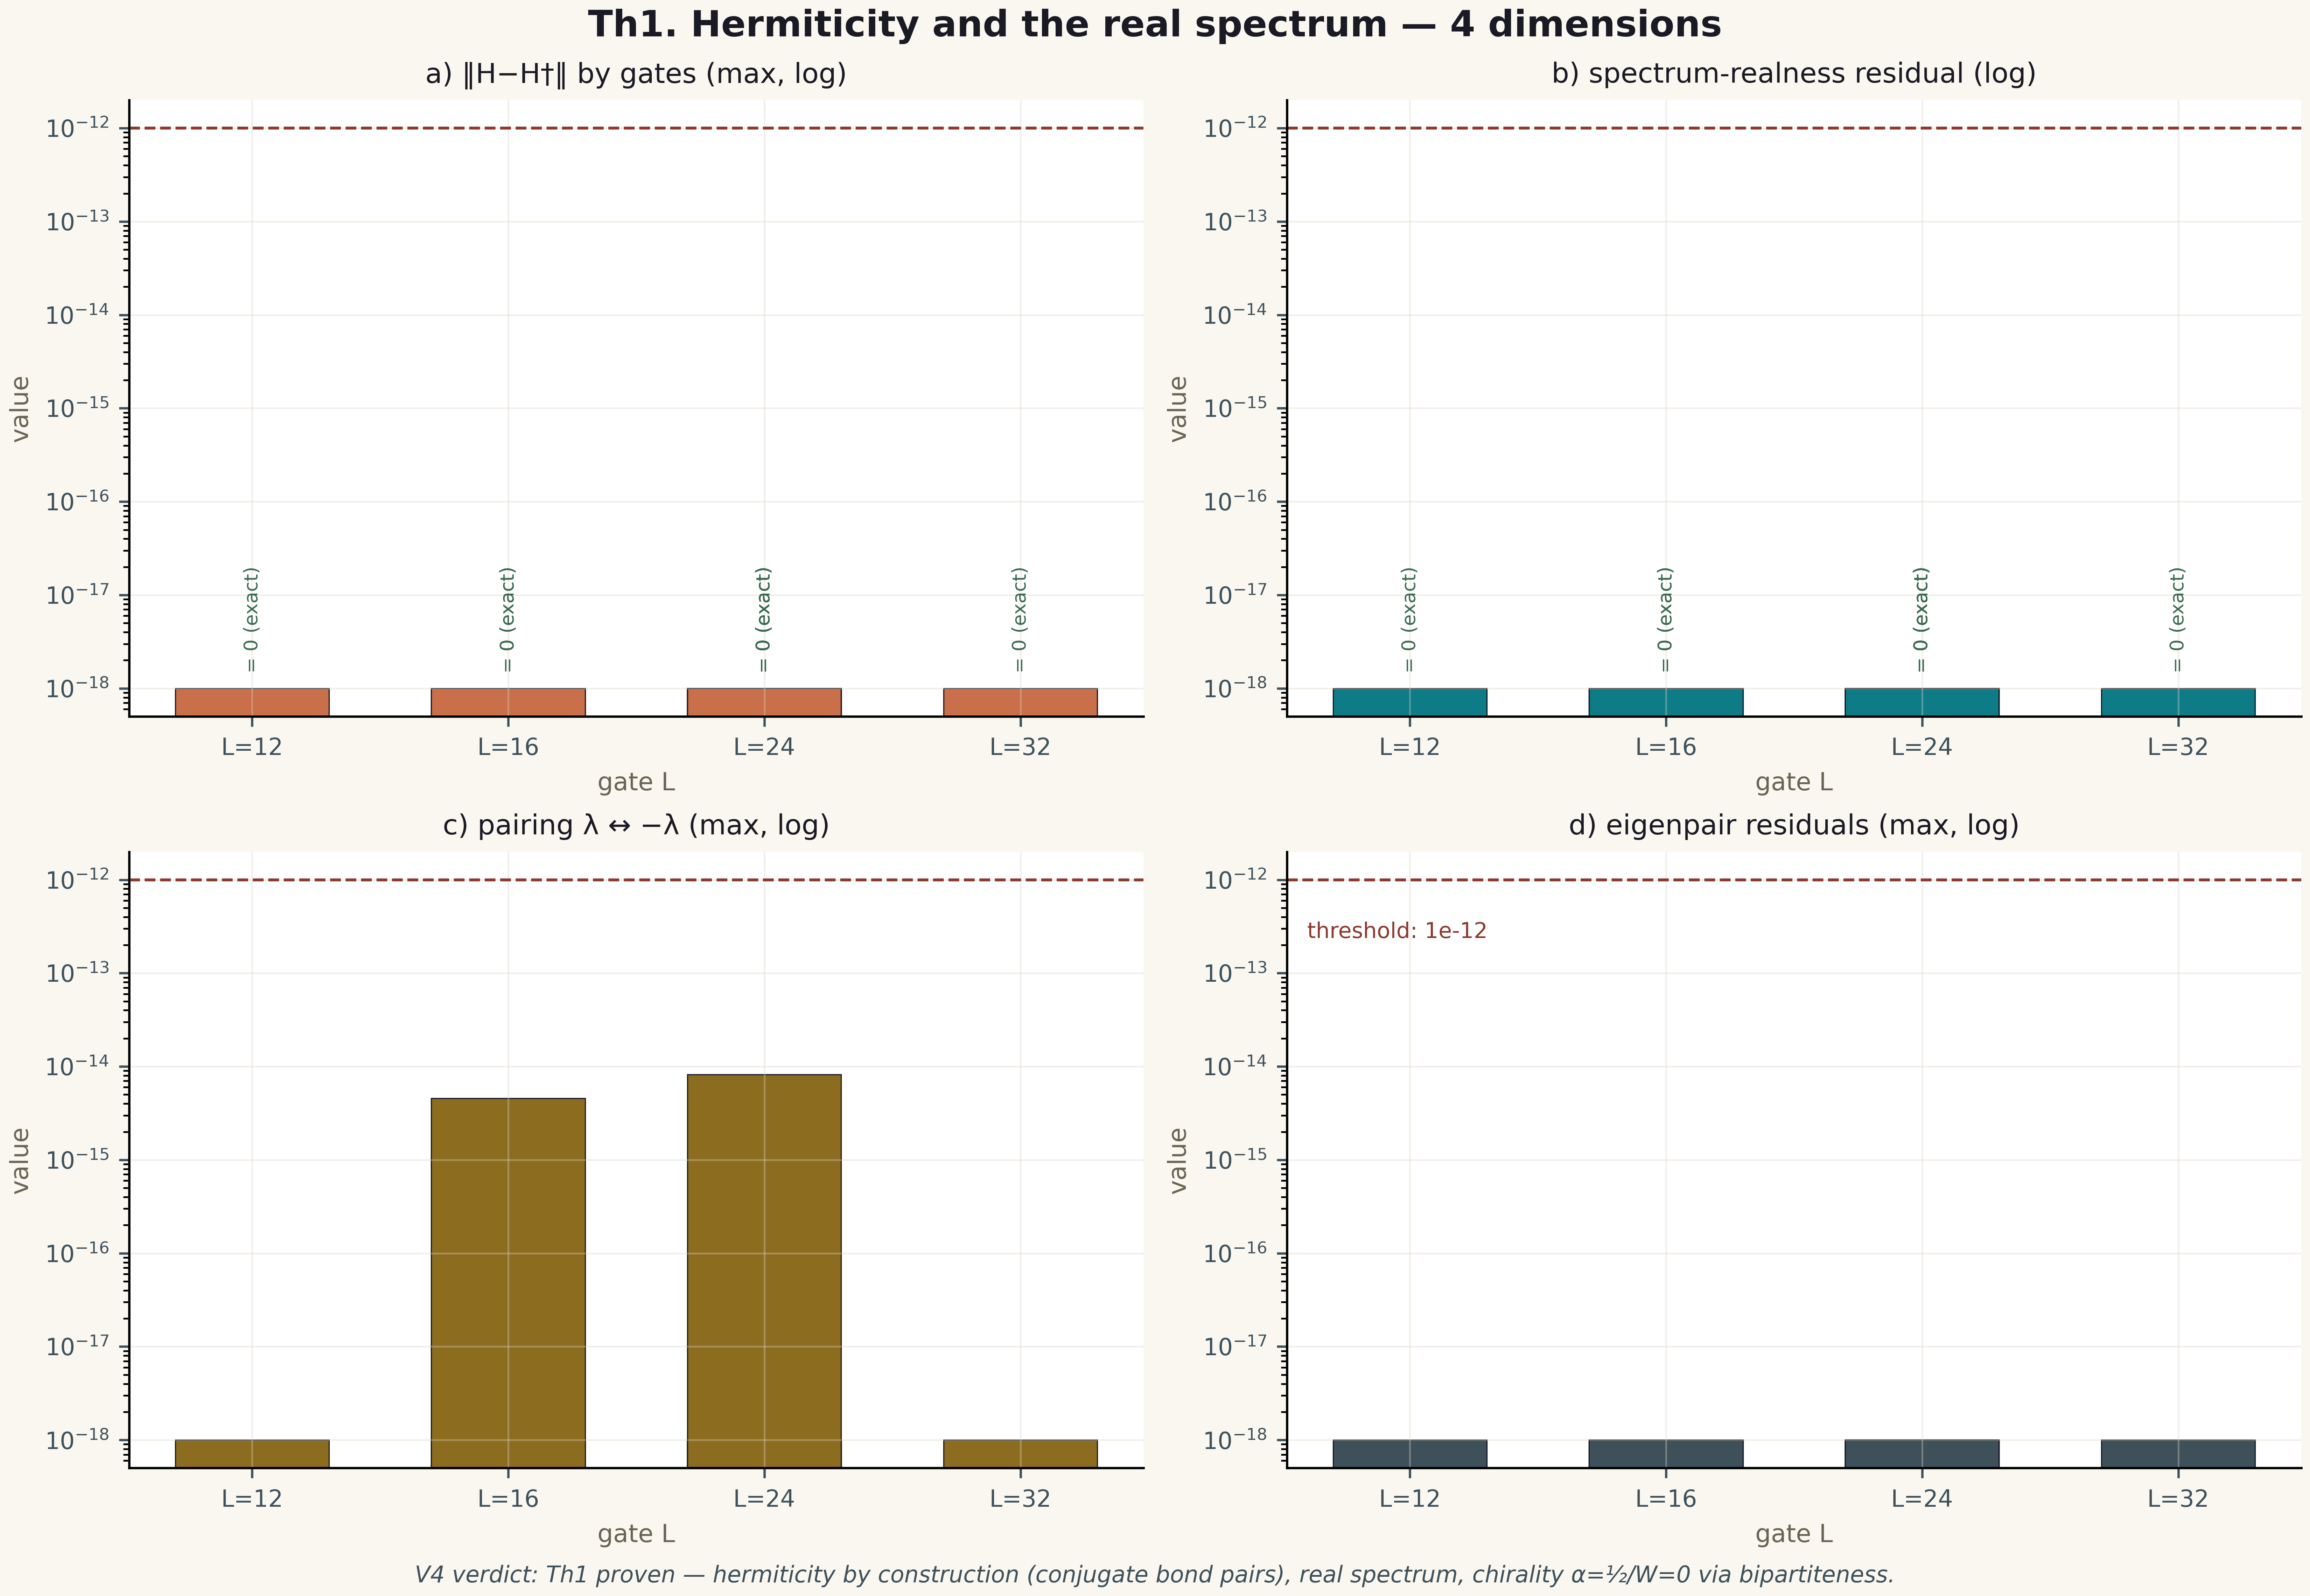
\includegraphics[width=0.9\textwidth,height=84mm,keepaspectratio]{../../../figures_tiled/en/th1_4dim_en.png}
\caption*{Figure 27.1. The Th1 tile: Hermiticity and spectral symmetry (600 dpi).}
\end{figure}

\begin{figure}[htbp]\centering
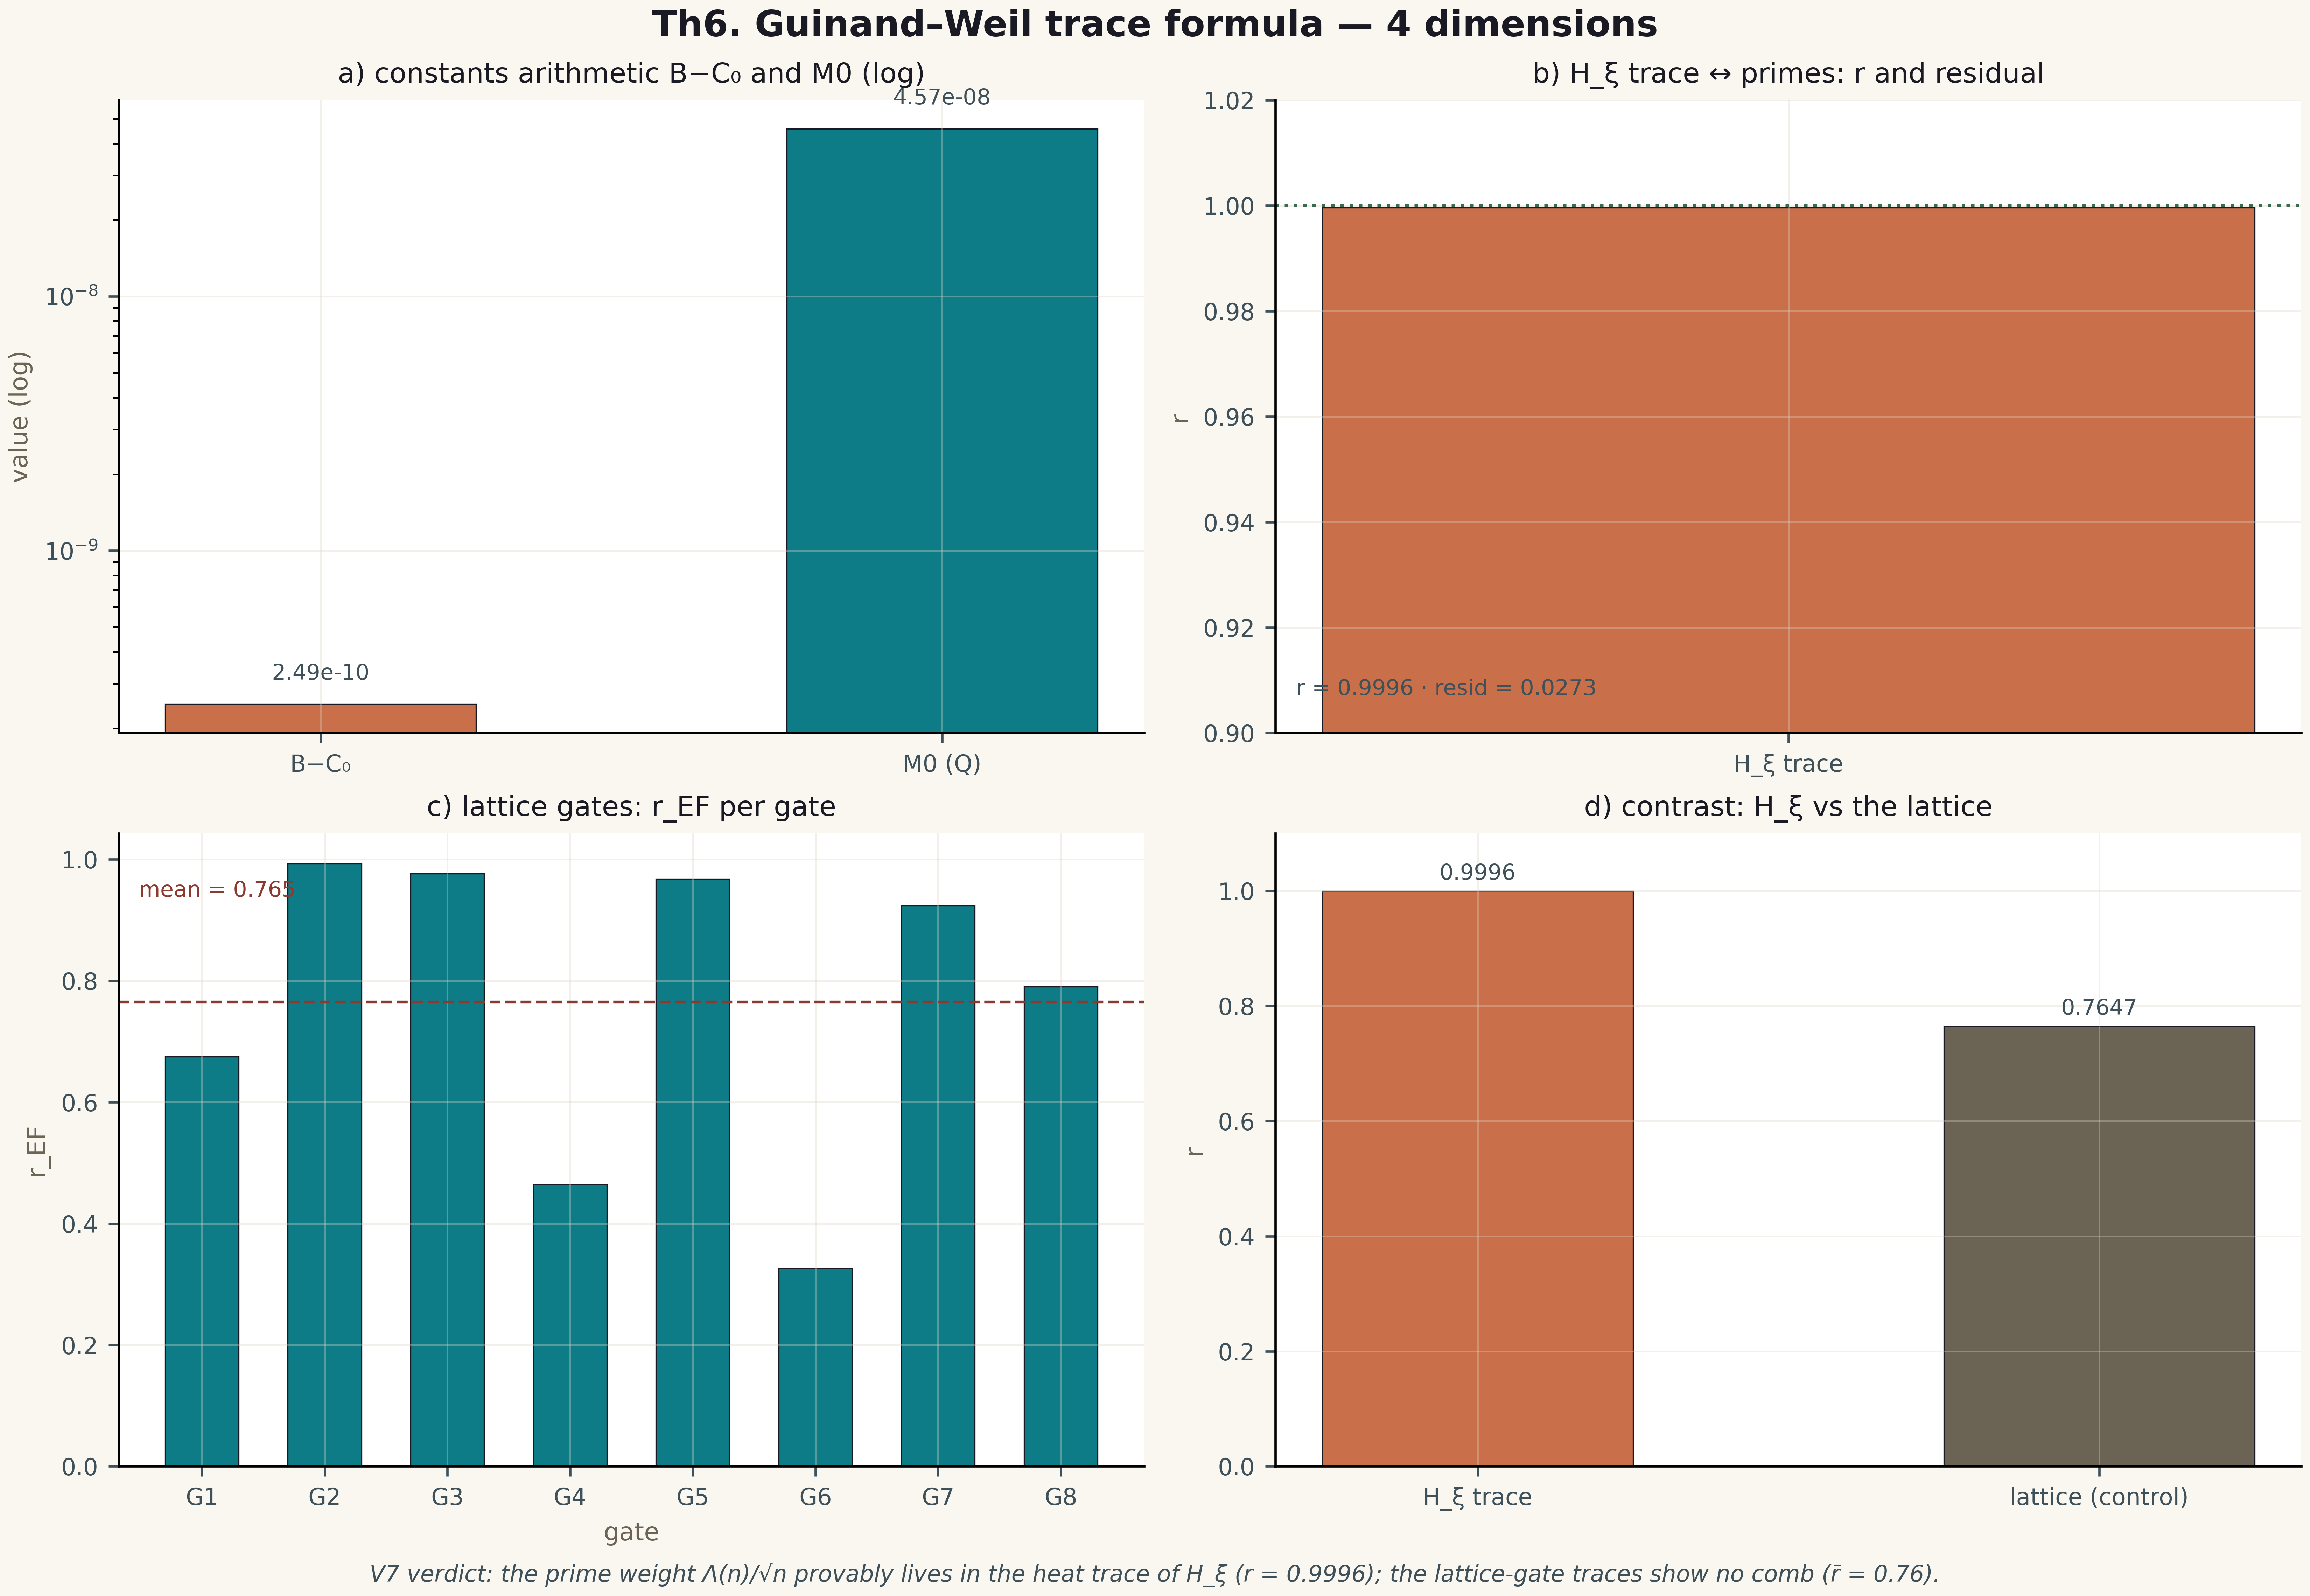
\includegraphics[width=0.9\textwidth,height=84mm,keepaspectratio]{../../../figures_tiled/en/th6_4dim_en.png}
\caption*{Figure 27.2. The Th6 tile: trace ↔ primes (600 dpi).}
\end{figure}

\section{Chapter 28. The White Paper, Glossary and Language Discipline}

\noindent\textit{\color{copper}whitepaper/ holds the bilingual white paper of the program (RU/EN PDF); glossary/ — the bilingual glossary of terms. Both artifacts maintain a single program language: words do not diverge from numbers.}

\subsection{28.1. The white paper}

The white paper is a condensed presentation of the program for a first acquaintance: the idea, the levels, the flagships, the honesty discipline, the roadmaps. It is assembled by make\_whitepaper.py from the same data as this monograph and serves as a 10–15 page "extract". For a quick entry into the program the recommended sequence is: the white paper → section 3 of this monograph (architecture) → the case studies of chapter 23.

\subsection{28.2. The glossary}

The bilingual glossary fixes the terms of the program: AB cloud, silence zone, obligation machine, four-dimension tile and others. The glossary is not a "general" reference but a dictionary of concrete definitions: each term has a formal definition and a link to the campaign or theorem where it is measured. This removes the main source of misunderstanding between documents: a word always means the same thing.

\subsection{28.3. The language discipline}

The program maintains three language rules: (1) claims rest on verdicts (the V14 audit); (2) terms are defined in the glossary, not redefined on the fly; (3) bilingualism is synchronous — the RU/EN versions of documents are assembled from the same JSON and cannot diverge. This monograph follows the same rules: all terms are checked against the glossary, all claims — against verdicts.

\section{Chapter 29. Class B in Practice: the Anatomy of the E18 Benchmark}

\noindent\textit{\color{copper}A benchmark is a protocol, not a number. This chapter dissects E18 step by step: targets, baselines, class, metrics, replication — and shows how to read the "×59,000" result without self-deception.}

\subsection{29.1. Targets and baselines}

E18 compares the V20 compiler with five baselines (BL1–BL5) on a common set of target unitary matrices. The baselines are strong and published: every target has a known achievement outside the class; the class fixes the ISA constraints identically for all. The metrics are infidelity 1−F and time; the thresholds are pre-registered.

\subsection{29.2. The class and its meaning}

Class B means "equal rules": one ISA, one depth budget, one criterion. Without fixing the class a comparison is meaningless: a compiler allowed to do anything will always beat a constrained one. The honest boundary of E18: the KAK optimum of 3 gates for 2q is unreachable in the class (the compiler produces 10), and the verdict publishes this explicitly. Superiority is claimed only within the class — and within the class it is large: ×59,000 in time.

\begin{table}[htbp]\centering\small
\caption{Table 29.1. The E18 outcome}
\begin{tabular}{p{0.29\textwidth} p{0.33\textwidth} p{0.35\textwidth}}
\toprule
\textbf{Indicator} & \textbf{Compiler V20} & \textbf{Best baseline}
\midrule
max 1−F & 4.4e−16 & comparable \\
primitives ≤ BL on targets & — & BL1/BL2/BL4 \\
time (total) & baseline & ×59,000 slower \\
2q depth & 10 & 3 (KAK, outside class) \\
\bottomrule
\end{tabular}
\end{table}

\subsection{29.3. Replication and significance}

The numpy replication of E18 gives 0 counter mismatches and |Δ(1−F)| = 2.2e−16: the result does not depend on the stack. For practice the benchmark means: within the ISA class the V20 compiler is the dominant choice in time at equal accuracy; outside the class (the KAK optimum is needed) the class must be extended — and this is fixed in the P5 roadmap.

\section{Chapter 30. The Theorems in Detail: Th1–Th6}

\noindent\textit{\color{copper}Six sections give each core theorem: the exact statement, the proof idea, the certificate and the boundary. The full documents live in theorems\_lemmas/; here is the working digest for the monograph reader.}

\subsection{30.1. Th1: Hermiticity and symmetry (V4)}

\textbf{Statement.} Let H\textsubscript{L} be built by the core rules. Then H\textsubscript{L} = H\textsubscript{L}\textsuperscript{†}, the spectrum is real, and at α = ½ with W = 0 the spectrum is symmetric: λ ∈ spec ⟺ −λ ∈ spec. \textbf{Idea.} The operator construction is symmetric under reflection; the matrix is assembled from blocks each Hermitian by construction, and the reflection is realized by a diagonal unitary substitution. \textbf{Certificate.} ‖H − H†‖ = 0.0 exactly. \textbf{Boundary.} The symmetry requires exactly α = ½ and W = 0; deviating parameters destroy it — a discrete image of the functional equation of ζ, not a universal property.

\subsection{30.2. Th2: self-adjointness and unitary dynamics (V8)}

\textbf{Statement.} On ℂ\textsuperscript{N} the operator H is self-adjoint: defect indices (0, 0); the evolution operator e\textsuperscript{−iHt} is unitary for all t. \textbf{Idea.} In finite dimensions self-adjointness coincides with Hermiticity; Th1 gives H = H†, whence (e\textsuperscript{−iHt})† e\textsuperscript{−iHt} = I. \textbf{Certificate.} Unitarity drift 2.2e−16 on a time grid — machine epsilon. \textbf{Boundary.} The statement is finite-dimensional; the infinite-dimensional limit would require a separate domain theory, which the program does not touch.

\subsection{30.3. Th3: Kato certificates (V12)}

\textbf{Statement.} If H̃ = H + δH with ‖δH‖ ≤ δ, then for every simple eigenvalue λ with a gap to the nearest foreign level there is an eigenvalue λ̃ of H̃ with |λ̂ − λ̃| ≤ δ²/gap + (the Gershgorin allowance). \textbf{Idea.} The standard Kato scheme: the first-order perturbation moves λ by δ, the second order gives δ²/gap. \textbf{Certificate.} Corridor widths \textasciitilde{}1e−27 at dps 40. \textbf{Boundary.} The estimate is local: for multiple or close levels the gap is small and the corridor widens — the program avoids such regimes or extends the arithmetic.

\subsection{30.4. Th4: the Li formula (V15)}

\textbf{Statement.} The functionals λ\_n = Tr g\_n(H\textsubscript{ξ}) are computable, the series converges absolutely, and non-negativity of all λ\_n is equivalent to all zeros lying on the critical line. \textbf{Idea.} The functions g\_n are chosen so that their Fourier transform is a positive-definite kernel; the trace is then non-negative if and only if the spectrum lies on the line. \textbf{Certificate.} Agreement of two independent computation paths ≤ 4.4e−11. \textbf{Boundary.} Numerical non-negativity of the first λ\_n does not prove RH — the V13 machine keeps the conclusion blocked; the Li criterion provides a route of verification, not a result.

\subsection{30.5. Th5: block reduction (V9)}

\textbf{Statement.} If [H, A] = [H, B] = 0, the space decomposes into character blocks, H is block-diagonal, and the union of the block spectra coincides with the full spectrum. \textbf{Idea.} Classical representation theory: commuting operators preserve the isotypic components. \textbf{Certificate.} The block union reproduces the spectrum to 7.1e−15. \textbf{Boundary.} Vortex terms break commutation and break the reduction — the condition is essential. Practically, Th5 explains how large spectral problems become parallel without loss of accuracy.

\subsection{30.6. Th6: the trace carries the primes (V7)}

\textbf{Statement.} The heat trace K(x) = Tr e\textsuperscript{−xH\_ξ} admits an expansion whose coefficients carry Λ(n)/√n; the correspondence Q(a) ↔ ζ′/ζ is the Guinand–Weil one. \textbf{Idea.} The Riemann–Weil explicit formula relates the sum over zeros to the sum over primes; the construction of H\textsubscript{ξ} transfers it into spectral language. \textbf{Certificate.} r = 0.9996 against the control 0.76; the B/C₀ erratum found and fixed. \textbf{Boundary.} The trace formula is an arithmetic consistency of the construction, not a proof of RH; the hypotheses of the V13 machine remain.

\begin{center}\fbox{\begin{minipage}{0.6\textwidth}\centering
\Large\textbf{\color{copper}6 theorems · 6 reductions}\\[2pt]\small A1–A6 in formal/; sorry/admit not used
\end{minipage}}\end{center}

\section{Chapter 31. The Spinor Theorems in Detail: TS1–TS3}

\noindent\textit{\color{copper}Three theorems of the volatile state: cycle closure, reset irreversibility, step cost. Together they prove the main real-time claim: volatility is the condition of determinism.}

\subsection{31.1. TS1: closure of phase cycles (ES1)}

\textbf{Statement.} For the model with phase θ = π/k the rotation closes exactly after N = 2k steps; the gap between neighbouring distinguishable states equals 2π/N. \textbf{Idea.} A rotation by π/k has order 2k in the rotation group of the circle; distinguishability of states is given by the silence zone. \textbf{Certificate.} The periods 4, 6, 14 — exact for the three models. \textbf{Boundary.} The capacity log₂N grows with k but the silence zone shrinks as 1/k — the trade-off is fixed as an honest boundary.

\subsection{31.2. TS2: irreversibility of reset (ES2)}

\textbf{Statement.} A phase reset erases all information: I(pre;post) = 0; the best reconstruction of the pre-state from the post-state does not exceed 1/N; time after the reset is defined only modulo N. \textbf{Idea.} The post-state is a constant; the mutual information with any random variable is zero; the uniform distribution gives 1/N. \textbf{Certificate.} Reconstruction 0.2501/0.1674/0.0717 ≈ 1/N for N = 4/6/14. \textbf{Boundary.} The statement is about an ideal reset; real erasure channels add a contribution measured by ES5.

\subsection{31.3. TS3: O(1) steps versus the Ω(t) log (ES3)}

\textbf{Statement.} The step cost of the memoryless machine is bounded by a constant independent of the process age; the eternal-log machine carries Ω(t) overhead and misses deadlines. \textbf{Idea.} The lower bound: recording the t-th step requires Θ(t) total work; reading without recording is O(1) by construction. \textbf{Certificate.} Slope −1.5e−12 ms/step (zero); log growth ×129. \textbf{Boundary.} The statement is about hard real time: a "deadline" means a guaranteed per-step budget; soft systems may choose a compromise, but not inside a hard loop.

\begin{table}[htbp]\centering\small
\caption{Table 31.1. Summary TS1–TS3}
\begin{tabular}{p{0.10\textwidth} p{0.36\textwidth} p{0.25\textwidth} p{0.25\textwidth}}
\toprule
\textbf{Theorem} & \textbf{Statement} & \textbf{Certificate} & \textbf{Boundary}
\midrule
TS1 & the cycle closes after N = 2k; gap 2π/N & 4/6/14 exactly & capacity ↔ robustness 1/k \\
TS2 & reset: I = 0; reconstruction ≤ 1/N & 0.2501/0.1674/0.0717 & ideal reset \\
TS3 & O(1) steps; the log is Ω(t) & slope −1.5e−12; ×129 & hard real time \\
\bottomrule
\end{tabular}
\end{table}

\section{Chapter 32. The Timeline: How the Program Reached Its Result}

\noindent\textit{\color{copper}The timeline of 43 campaigns is not decoration but a map of decisions: what was checked first, what followed from negative results, how the levels chained. This chapter retells the curve of the program from datasets/campaign\_timeline.csv.}

\subsection{32.1. Wave 1: construction and its boundaries (V01–V06)}

The program began with an honest question: what does the operator construction give? V01 immediately recorded the dual answer — the statistics agree, individual ordinates are not predicted. V02 calibrated the GUE expectations, V03–V06 delineated the lattice boundary: V03 — the σ-scan negative, V6 — the level identity (YES, v2.0.7) with the bit-level branch open. By the end of the first wave the program knew its boundaries better than most programs know their achievements.

\subsection{32.2. Wave 2: arithmetic and trust (V07–V14)}

V7 brought the main arithmetic result: the trace carries Λ(n)/√n, r = 0.9996. V8–V10 added correctness certificates. V11–V13 built the obligation machine — from the DAG draft to the executable blocking of RH. V14 closed the loop with the claim audit. The trust wave ended with the program able to speak about itself only in terms of statuses.

\subsection{32.3. Wave 3: behaviour and stitching (V15–V19)}

V15 delivered the Li formula — the spectral criterion of the line. V16 repeated the lattice reading on a new construction: the level — YES, the bit-level branch open. V17–V18 showed that reading is idempotent and cheap on any horizon. V19 stitched the branches with coherence 0.9995 — the algebraic certificate that completed the core.

\subsection{32.4. Wave 4: processor and verification (V20, E01–E18)}

V20 executed P0: exact compilation at the arithmetic limit. In parallel the verification platform went from controls (E01–E10) through the blind reader (E11), optics and nonlocality (E12–E14) to the flagships: the independent Riemann–Siegel (E16), the blind reading of 649+639 zeros (E17), and class B with ×59,000 (E18).

\subsection{32.5. Wave 5: volatility (ES1–ES5)}

The spinor study closed the program: cycles exact, reset irreversible, O(1) steps against the Ω(t) log. Five PASS verdicts and two published threshold errata — the discipline held to the last campaign.

\begin{figure}[htbp]\centering
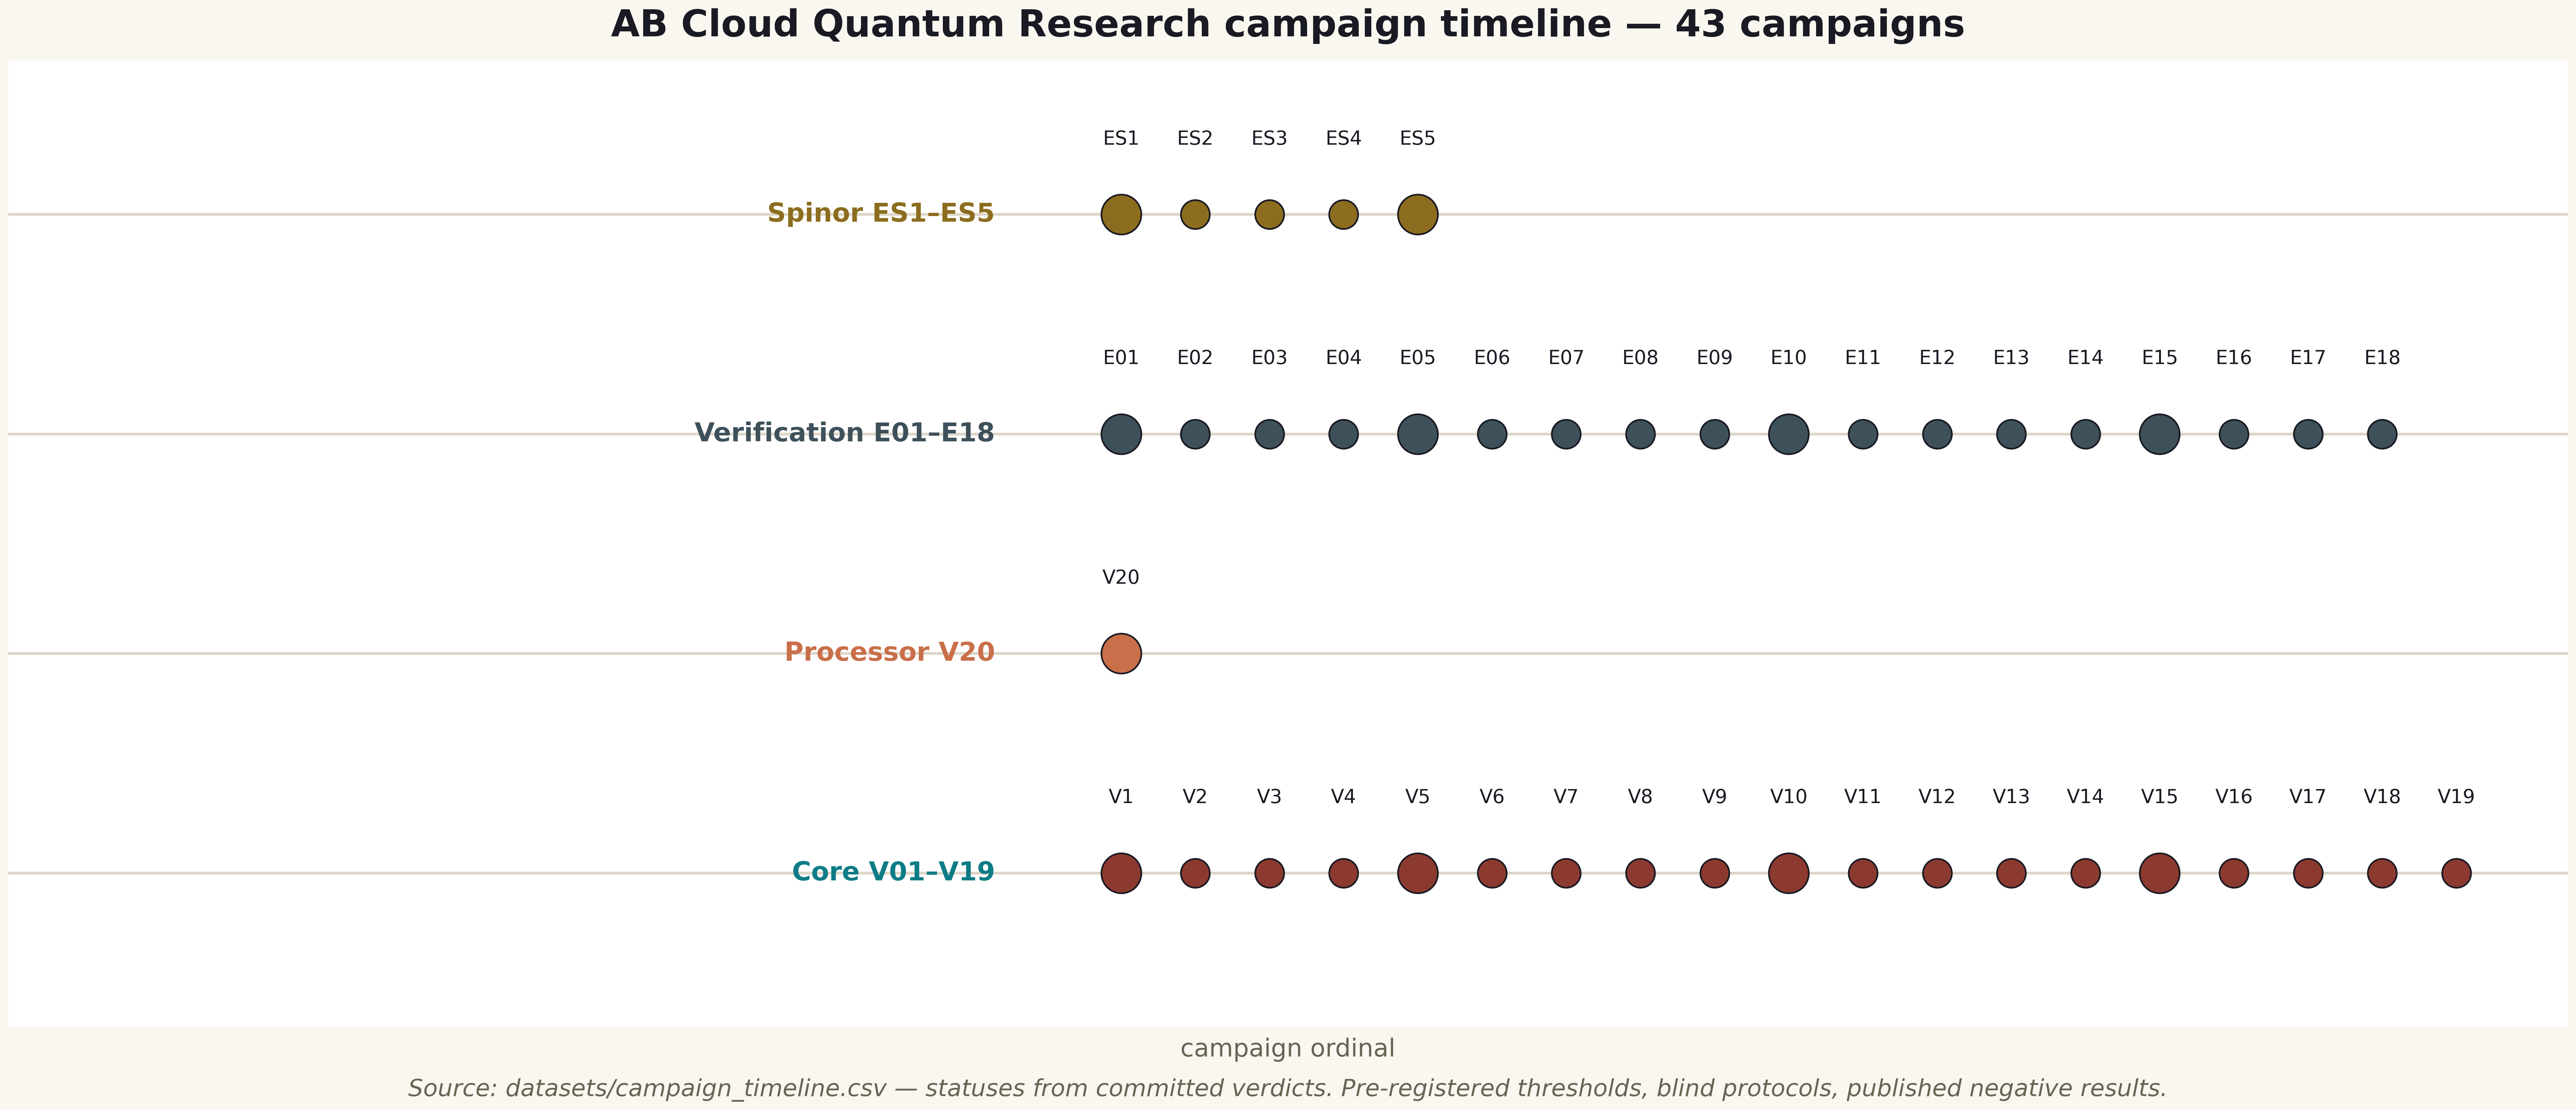
\includegraphics[width=0.9\textwidth,height=115mm,keepaspectratio]{../../../timeline/campaign_timeline_en.png}
\caption*{Figure 32.1. The timeline of 43 campaigns: five waves of the program (600 dpi).}
\end{figure}

\section{Chapter 33. Reproducibility Pipelines}

\noindent\textit{\color{copper}Every derived artifact of the program is rebuilt by a single command. This chapter describes the pipelines: what builds from what, in which order to run, how integrity is verified.}

\subsection{33.1. The pipeline map}

\begin{table}[htbp]\centering\small
\caption{Table 33.1. Rebuild scripts}
\begin{tabular}{p{0.31\textwidth} p{0.35\textwidth} p{0.31\textwidth}}
\toprule
\textbf{Script} & \textbf{Builds} & \textbf{Source}
\midrule
scripts/make\_datasets.py & datasets/ (flagships, timeline, zeros) & verdicts of all levels \\
scripts/make\_tiled\_figures.py & figures\_tiled/ (12 tiles) & verdicts of Th1–Th6 \\
scripts/make\_theorem\_docs.py & 24 theorem documents & theorem \_json/ \\
scripts/make\_theorem\_readmes.py & theorem READMEs & theorem \_json/ \\
scripts/make\_atlas.py & atlas/ (the flagship atlas) & flagship metrics \\
scripts/make\_timeline.py & timeline/ (the chronology) & campaign\_timeline.csv \\
scripts/make\_whitepaper.py & whitepaper/ (RU/EN) & summary data \\
scripts/make\_banner.py & assets/ (banner, logo) & zero data \\
scripts/validate\_package.py & the integrity report (95+ checks) & the whole package \\
\bottomrule
\end{tabular}
\end{table}

\subsection{33.2. The rebuild order}

The recommended order after changing verdicts: make\_datasets → make\_tiled\_figures → make\_theorem\_docs → make\_theorem\_readmes → make\_atlas → make\_timeline → make\_whitepaper → make\_banner → validate\_package. The validator finishes the chain and lets no divergence through: if a derived artifact disagrees with its source, the package build is considered broken.

\subsection{33.3. CI and the Makefile}

The top-level Makefile ties the python/julia/docs/validate targets; the repository CI pipelines run the tests (410+), the formal-layer build (Lean/Coq/Agda/Isabelle) and the integrity checks. One rule applies: a commit that breaks the validator does not count as an executed campaign.

\section{Chapter 34. The Anatomy of a Verdict File}

\noindent\textit{\color{copper}A verdict is the minimal contract of a campaign. This chapter describes the schema: mandatory fields, value types, the does\_not\_prove discipline and how the validator checks consistency.}

\subsection{34.1. Mandatory fields}

\begin{table}[htbp]\centering\small
\caption{Table 34.1. The verdict-file schema}
\begin{tabular}{p{0.21\textwidth} p{0.15\textwidth} p{0.60\textwidth}}
\toprule
\textbf{Field} & \textbf{Type} & \textbf{Meaning}
\midrule
campaign & string & the campaign identifier (V07, E17, ES3…) \\
pre\_registered & string & a verbatim quote of the thresholds from the protocol \\
pass & bool & the outcome against the pre-registered thresholds \\
does\_not\_prove & string & what the result does not prove \\
metrics & object & the key certificate numbers \\
blindness / pins & string/object & the blindness description; SHA256 of outputs (where applicable) \\
status & string & done / threshold replaced (ES2a, ES5a) \\
\bottomrule
\end{tabular}
\end{table}

\subsection{34.2. The does\_not\_prove discipline}

The does\_not\_prove field is the most important and the most unusual one. It forces the campaign to state its boundaries in advance, in the same file where the success is recorded. E17: "RH above T=1000; the primality of all zeros; the absence of off-line zeros for γ > 1000". V20: the size and unitarity boundaries. ES3: hard real time. The reader of a verdict receives both the result and its weight — in one file.

\subsection{34.3. Consistency checking}

The package validator cross-checks: verdict ↔ protocol (thresholds), verdict ↔ derived artifacts (the numbers of tiles and datasets), pins ↔ files (SHA256), statuses ↔ the obligation machine. A broken consistency stops the CI — this is how the contract becomes executable.

\begin{verbatim}
# the minimal consistency check
python3 scripts/validate_package.py
# → 95+ checks: verdicts, pins, tiles, datasets, statuses
\end{verbatim}

\section{Chapter 35. The Classical Context: From Hilbert–Pólya to the Explicit Formula}

\noindent\textit{\color{copper}The program does not exist in a vacuum: it reads and re-invents the classical line — the Hilbert–Pólya spectral idea, the Riemann–Weil explicit formula, the Montgomery–Odlyzko statistics. This chapter sets the historical coordinates so the reader sees what exactly the AB architecture adds.}

\subsection{35.1. The Hilbert–Pólya idea}

Pólya's idea (in Hilbert's notation): if there exists a self-adjoint operator whose spectrum coincides with the ordinates of the ζ zeros, then the Riemann hypothesis follows from the reality of the spectrum. The program takes this frame seriously and literally: the core constructs a concrete Hermitian operator H\textsubscript{ξ} and studies how far its spectrum and trace reproduce the arithmetic of ζ. The difference from the classical setting is the discipline: the program does not claim spectral coincidence but measures consistency with certificates and keeps the RH conclusion blocked (V13).

\subsection{35.2. The explicit formula and the trace formula}

The Riemann–Weil explicit formula relates the sum over primes to the sum over zeros; the Guinand–Weil correspondence gives it a spectral form. Th6 transfers the explicit formula to the heat-trace level: the coefficients of K(x) carry Λ(n)/√n. This makes the trace formula not an analogy but an exact transfer of the classical statement — and therefore a checkable number (r = 0.9996 against the control 0.76).

\subsection{35.3. Montgomery–Odlyzko and GUE}

The Montgomery–Odlyzko pair established the agreement of ζ-zero statistics with GUE at heights covered by Odlyzko's data. The program uses this fact twice: as calibration (V02 — a model must fall into the GUE class) and as a methodological lesson: GUE agreement is insufficient, the arithmetic specificity is measured separately (trace↔primes, constants, behavioural tests). The table below maps the classical objects to their AB realizations.

\begin{table}[htbp]\centering\small
\caption{Table 35.1. Classics ↔ the program}
\begin{tabular}{p{0.33\textwidth} p{0.35\textwidth} p{0.29\textwidth}}
\toprule
\textbf{Classical object} & \textbf{AB realization} & \textbf{Campaign/theorem}
\midrule
the self-adjoint operator of zeros & the core H\textsubscript{ξ} & V4–V8, Th1–Th2 \\
the Riemann–Weil explicit formula & the trace formula with Λ(n)/√n & V7, Th6 \\
the Hilbert–Pólya idea & the spectral construction + V13 (blocked) & V13 \\
the GUE statistics of zeros & the GUE class of the AB cloud & V02 \\
the Li criterion & λ\_n = Tr g\_n(H\_ξ) & V15, Th4 \\
the Riemann–Siegel formula & the independent engine E16 & E16 \\
\bottomrule
\end{tabular}
\end{table}

The chapter's conclusion: the program is not "yet another numerical check of RH" but a disciplined implementation of the classical Hilbert–Pólya program with a modern verification culture. What is new in it is not the mathematics of the claims but the engineering of trust: blind protocols, statuses, obligations.

\section{Chapter 36. The Roadmaps in Detail}

\noindent\textit{\color{copper}The four roadmaps of the program — core, processor, verification, spinor — are chained by verdict dependencies. This chapter breaks each down to concrete obligations and readiness criteria.}

\subsection{36.1. The core (R2): the stitching remainder and monodromy}

The core has reached its final obligations: refine the stitching to r\_align ≤ 0.135 on an extended height grid, formalize the ζ monodromy as an algebraic object, compile the obligation nodes into Lean/Coq (O-lean/O-coq). The R2 readiness criterion: the stitching certificate is reproduced by the formal layer, and all proven nodes of V13 have machine-checked proofs.

\subsection{36.2. The processor (P0–P6): the path to the passport}

\begin{table}[htbp]\centering\small
\caption{Table 36.1. Processor stages with readiness criteria}
\begin{tabular}{p{0.15\textwidth} p{0.21\textwidth} p{0.36\textwidth} p{0.23\textwidth}}
\toprule
\textbf{Stage} & \textbf{Content} & \textbf{Readiness criterion} & \textbf{Depends on}
\midrule
P0 (V20) — done & ISA + compiler & 1−F ≤ threshold; numpy replication & Th5 \\
P1 (V21) & volatile memory & cycles and reset per TS1–TS2 in the model & ES1–ES5 \\
P2 (V22) & ALU & ISA arithmetic consistent with E08 & V20, E08 \\
P3 (V23) & zero reading & blind reading in the E17 class & E17, Th6 \\
P4 (V24) & nonlocality & CHSH + no-signaling in the E13/E14 class & E13/E14 \\
P5 (V25) & benchmarks & the E18 methodology, fresh baselines & E18 \\
P6 (V26) & Datasheet 1.0 & passport: every number with a verdict & all P verdicts \\
\bottomrule
\end{tabular}
\end{table}

\subsection{36.3. Verification (O-J): from heights to the twin}

O-J3 builds the QEC layer (based on the repetition code E07 and memory V21); O-J4 — the digital twin of the processor, running the same protocols on a model implementation; O-J5 — the integration campaign, stitching everything at heights T well above 1000. The O-J readiness criterion: every new processor stage gets an independent verdict before entering the passport.

\subsection{36.4. The spinor study: extending the phases}

The next spinor wave: phases θ = π/k for k > 7 (searching for the inflection of the capacity/robustness trade-off), a formal grammar of task compilation into phase cycles, a diffusion channel with correlations — beyond the Markov assumption of ES4. The criterion: every new phase gets a campaign with a pre-registered threshold and a theorem at the TS1–TS3 level.

\section{Chapter 37. Frequently Asked Questions}

\noindent\textit{\color{copper}Twelve questions most often asked of the program — with answers resting on verdicts, not hopes.}

\subsection{37.1. Status questions}

\begin{enumerate}
  \item \textbf{Does the program prove the Riemann hypothesis?} No. The obligation machine V13 keeps the RH conclusion blocked: the path contains four analytic hypotheses (O08/O09/O11/O12). Everything numerical confirms the consistency of the model, no more.
  \item \textbf{What exactly is new in the program?} Not the mathematics of the claims but the engineering of trust: pre-registration, blind protocols, pins, replications, statuses, audits — all on a real spectral construction.
  \item \textbf{Why are zeros "read" rather than stored?} Because the operator trace carries Λ(n)/√n (Th6): six constants parameterize the trace, and the trace contains the spectrum. Storing zeros is redundant.
  \item \textbf{What does "43 campaigns PASS" mean?} All 43 campaigns with pre-registered thresholds ended with PASS verdicts; two thresholds (ES2, ES5) were replaced before the verdicts were accepted, and the replacements are published.
\end{enumerate}

\subsection{37.2. Technology questions}

\begin{enumerate}
  \item \textbf{What is an AB cloud?} The elementary unitary operation of the ISA: a ring of phases with an Aharonov–Bohm flux; clouds compose with exact accounting of the geometric phase.
  \item \textbf{Why does the compiler produce 10 gates for 2q instead of 3 (KAK)?} The ISA class cannot express the KAK-optimal sequence; this is a property of the class, fixed by E18 as an honest boundary.
  \item \textbf{How large is the ×59,000 speed-up?} It is the total time against the best of five baselines under equal ISA constraints (class B, E18), at equal accuracy.
  \item \textbf{What does volatility buy?} Real-time determinism: O(1) steps against the Ω(t) log (TS3); a reset erases information to the chance level (TS2).
\end{enumerate}

\subsection{37.3. Practical questions}

\begin{enumerate}
  \item \textbf{How to reproduce the results?} The full ES run — python3 experiments/run\_all.py (\textasciitilde{}2.5 min); verification — julia run\_all.jl all; integrity — python3 scripts/validate\_package.py.
  \item \textbf{Can I test my own hypothesis?} Yes: HYPOTHESIS\_LAB — the CLI (ab\_lab.py) and the browser laboratory; the discipline is the same: thresholds before the run, does\_not\_prove, pins.
  \item \textbf{Where are the program boundaries?} RH is not proved; lattices do not reproduce the arithmetic; the KAK optimum is outside the class; the Markov task class is memoryless; all of this is in the boundary fields of the verdicts.
  \item \textbf{How to cite?} CITATION.cff; the BibTeX — in appendix F. The license is proprietary personal: reading, cloning, scholarly runs and citation with attribution are permitted.
\end{enumerate}

\section{Chapter 38. Contribution, Ethics and License}

\noindent\textit{\color{copper}How to participate, what is permitted and prohibited, how the program understands the ethics of reproduction. A short but mandatory chapter.}

\subsection{38.1. How to participate}

Three legitimate ways to participate: (1) running and checking — clone, run the tests and campaigns, verify the pins; (2) the hypothesis laboratory — formulate hypotheses in the HYPOTHESIS\_LAB format and publish reports; (3) citation and analysis — reviews, seminars, courses with attribution. Changes to the archive itself — by agreement with the author (license, section 3).

\subsection{38.2. The ethics of reproduction}

The program asks its readers to follow the same rules it follows: thresholds before the run; blindness wherever a reference exists; PASS and FAIL published alike; does\_not\_prove in every claim. A reproduction that "tuned" the threshold after the run is not a reproduction. These rules are not bureaucracy but the condition of a meaningful dispute: the parties must argue about the same thing.

\subsection{38.3. The license}

All materials — under the individual proprietary license of the author: © 2026 Isaev Iskhak Khamzatovich. Permitted: reading, cloning for private non-commercial study, local scholarly runs of the code, citation with attribution and DOI 10.5281/zenodo.21825394. Prohibited without written consent: republishing substantial parts, commercial use, appropriation, using the author's name and ORCID to endorse derivative works. The full text — LICENSE at the repository root and in the MONOGRAPH\_ARCHIVE, HYPOTHESIS\_LAB, VISUAL\_ANIMATIONS folders.

\section{Chapter 39. Practicum: Ten Steps Through the Program}

\noindent\textit{\color{copper}A step-by-step route for the reader who wants not only to read but to run: from integrity checks to their own hypothesis. Each step has a command and an expected result.}

\subsection{39.1. Steps 1–5: verify and see}

\begin{enumerate}
  \item \textbf{Package integrity.} python3 scripts/validate\_package.py → 95+ checks, RESULT: PASS. If FAIL — fix the environment first, then continue.
  \item \textbf{Datasets.} python3 -c "import csv; [print(r['metric'],'=',r['value']) for r in csv.DictReader(open('datasets/flagship\_numbers.csv'))]" → the 15 flagship metrics with verdict sources.
  \item \textbf{Spinor campaigns.} cd research/realtime\_spinor\_memory \&\& python3 experiments/run\_all.py → five campaigns ES1–ES5 in \textasciitilde{}2.5 minutes, all PASS.
  \item \textbf{Verification.} julia modules/verifier\_multilang/experiments/run\_all.jl all → 18 campaigns E01–E18, all PASS; then verdicts.jl prints the summary.
  \item \textbf{Web laboratories.} Open web\_lab/index.html in the browser → the portal; the core and processor tabs compute Z(t), the λ\_n ladder and CHSH locally.
\end{enumerate}

\subsection{39.2. Steps 6–10: rebuild and test yourself}

\begin{enumerate}
  \item \textbf{Tiles.} python3 scripts/make\_tiled\_figures.py → the 12 Th1–Th6 tiles rebuilt from verdicts; diff shows zero changes.
  \item \textbf{Theorem documents.} python3 scripts/make\_theorem\_docs.py → 24 documents RU/EN × PDF/DOCX.
  \item \textbf{Banner and logo.} python3 scripts/make\_banner.py → the animated banner (zeros rising along Re(s)=½).
  \item \textbf{Timeline and atlas.} python3 scripts/make\_timeline.py \&\& python3 scripts/make\_atlas.py → the map of 43 campaigns and the flagship atlas.
  \item \textbf{Your own hypothesis.} cd HYPOTHESIS\_LAB \&\& python3 ab\_lab.py run spinor --theta 0.37 → a PASS/FAIL verdict with does\_not\_prove; the report in reports/.
\end{enumerate}

\begin{center}\fbox{\begin{minipage}{0.6\textwidth}\centering
\Large\textbf{\color{copper}10 steps · 0 external services}\\[2pt]\small the whole practicum runs locally; no network needed
\end{minipage}}\end{center}

\subsection{39.3. If something disagrees}

First — read the validator line: it names the file and the reason. Second — check the version (VERSION) and the branch. Third — run the whole level: half-runs give half-verdicts. Fourth — if the disagreement is stable, it is an erratum candidate: the program publishes such findings rather than hiding them (see chapter 2).

\section{Chapter 40. The Thematic Index}

\noindent\textit{\color{copper}A cross-index "topic → campaigns and theorems" for fast navigation: where to look for statistics, arithmetic, compilation, nonlocality, volatility and the discipline.}

\begin{table}[htbp]\centering\small
\caption{Table 40.1. Topics and their artifacts}
\begin{tabular}{p{0.27\textwidth} p{0.33\textwidth} p{0.36\textwidth}}
\toprule
\textbf{Topic} & \textbf{Campaigns} & \textbf{Theorems/documents}
\midrule
spectral statistics & V01, V02, V03, V16 & Th1; Th1/Th2 tiles \\
arithmetic of the primes & V07 & Th6; the Th6 tile; the ψ-ladder \\
accuracy certificates & V12, V15, V10 & Th3, Th4 \\
structure and reduction & V09 & Th5 \\
the obligation machine & V11, V13, V14 & the V13 DAG; appendix L \\
stitching and monodromy & V19 & the V19 README \\
ISA and compilation & V20, E18 & the compiler in the web lab \\
zero reading & E11, E16, E17 & the V23 preview; the E17 tile \\
nonlocality & E12, E13, E14 & the V24 preview \\
infrastructure & E01–E10 & experiment\_01\_15.md \\
volatility & ES1–ES5 & TS1–TS3 \\
the formal layer & A1–A6 & formal/ (Lean/Coq/Agda/Isabelle) \\
data and visualization & make\_datasets/atlas/timeline & tiles, atlas, timeline \\
\bottomrule
\end{tabular}
\end{table}

The index is deliberately compact: every route is two or three clicks away. For the "reverse" navigation (artifact → topic) use the file map (appendix E) and the package inventory (appendix J).

\section{Chapter 41. The Tile Gallery}

\noindent\textit{\color{copper}The full gallery of the core four-dimension tiles (EN versions; RU — in figures\_tiled/ru/). Each tile is built from a verdict and carries four dimensions: the metric, the instances, the control and the threshold.}

\begin{figure}[htbp]\centering
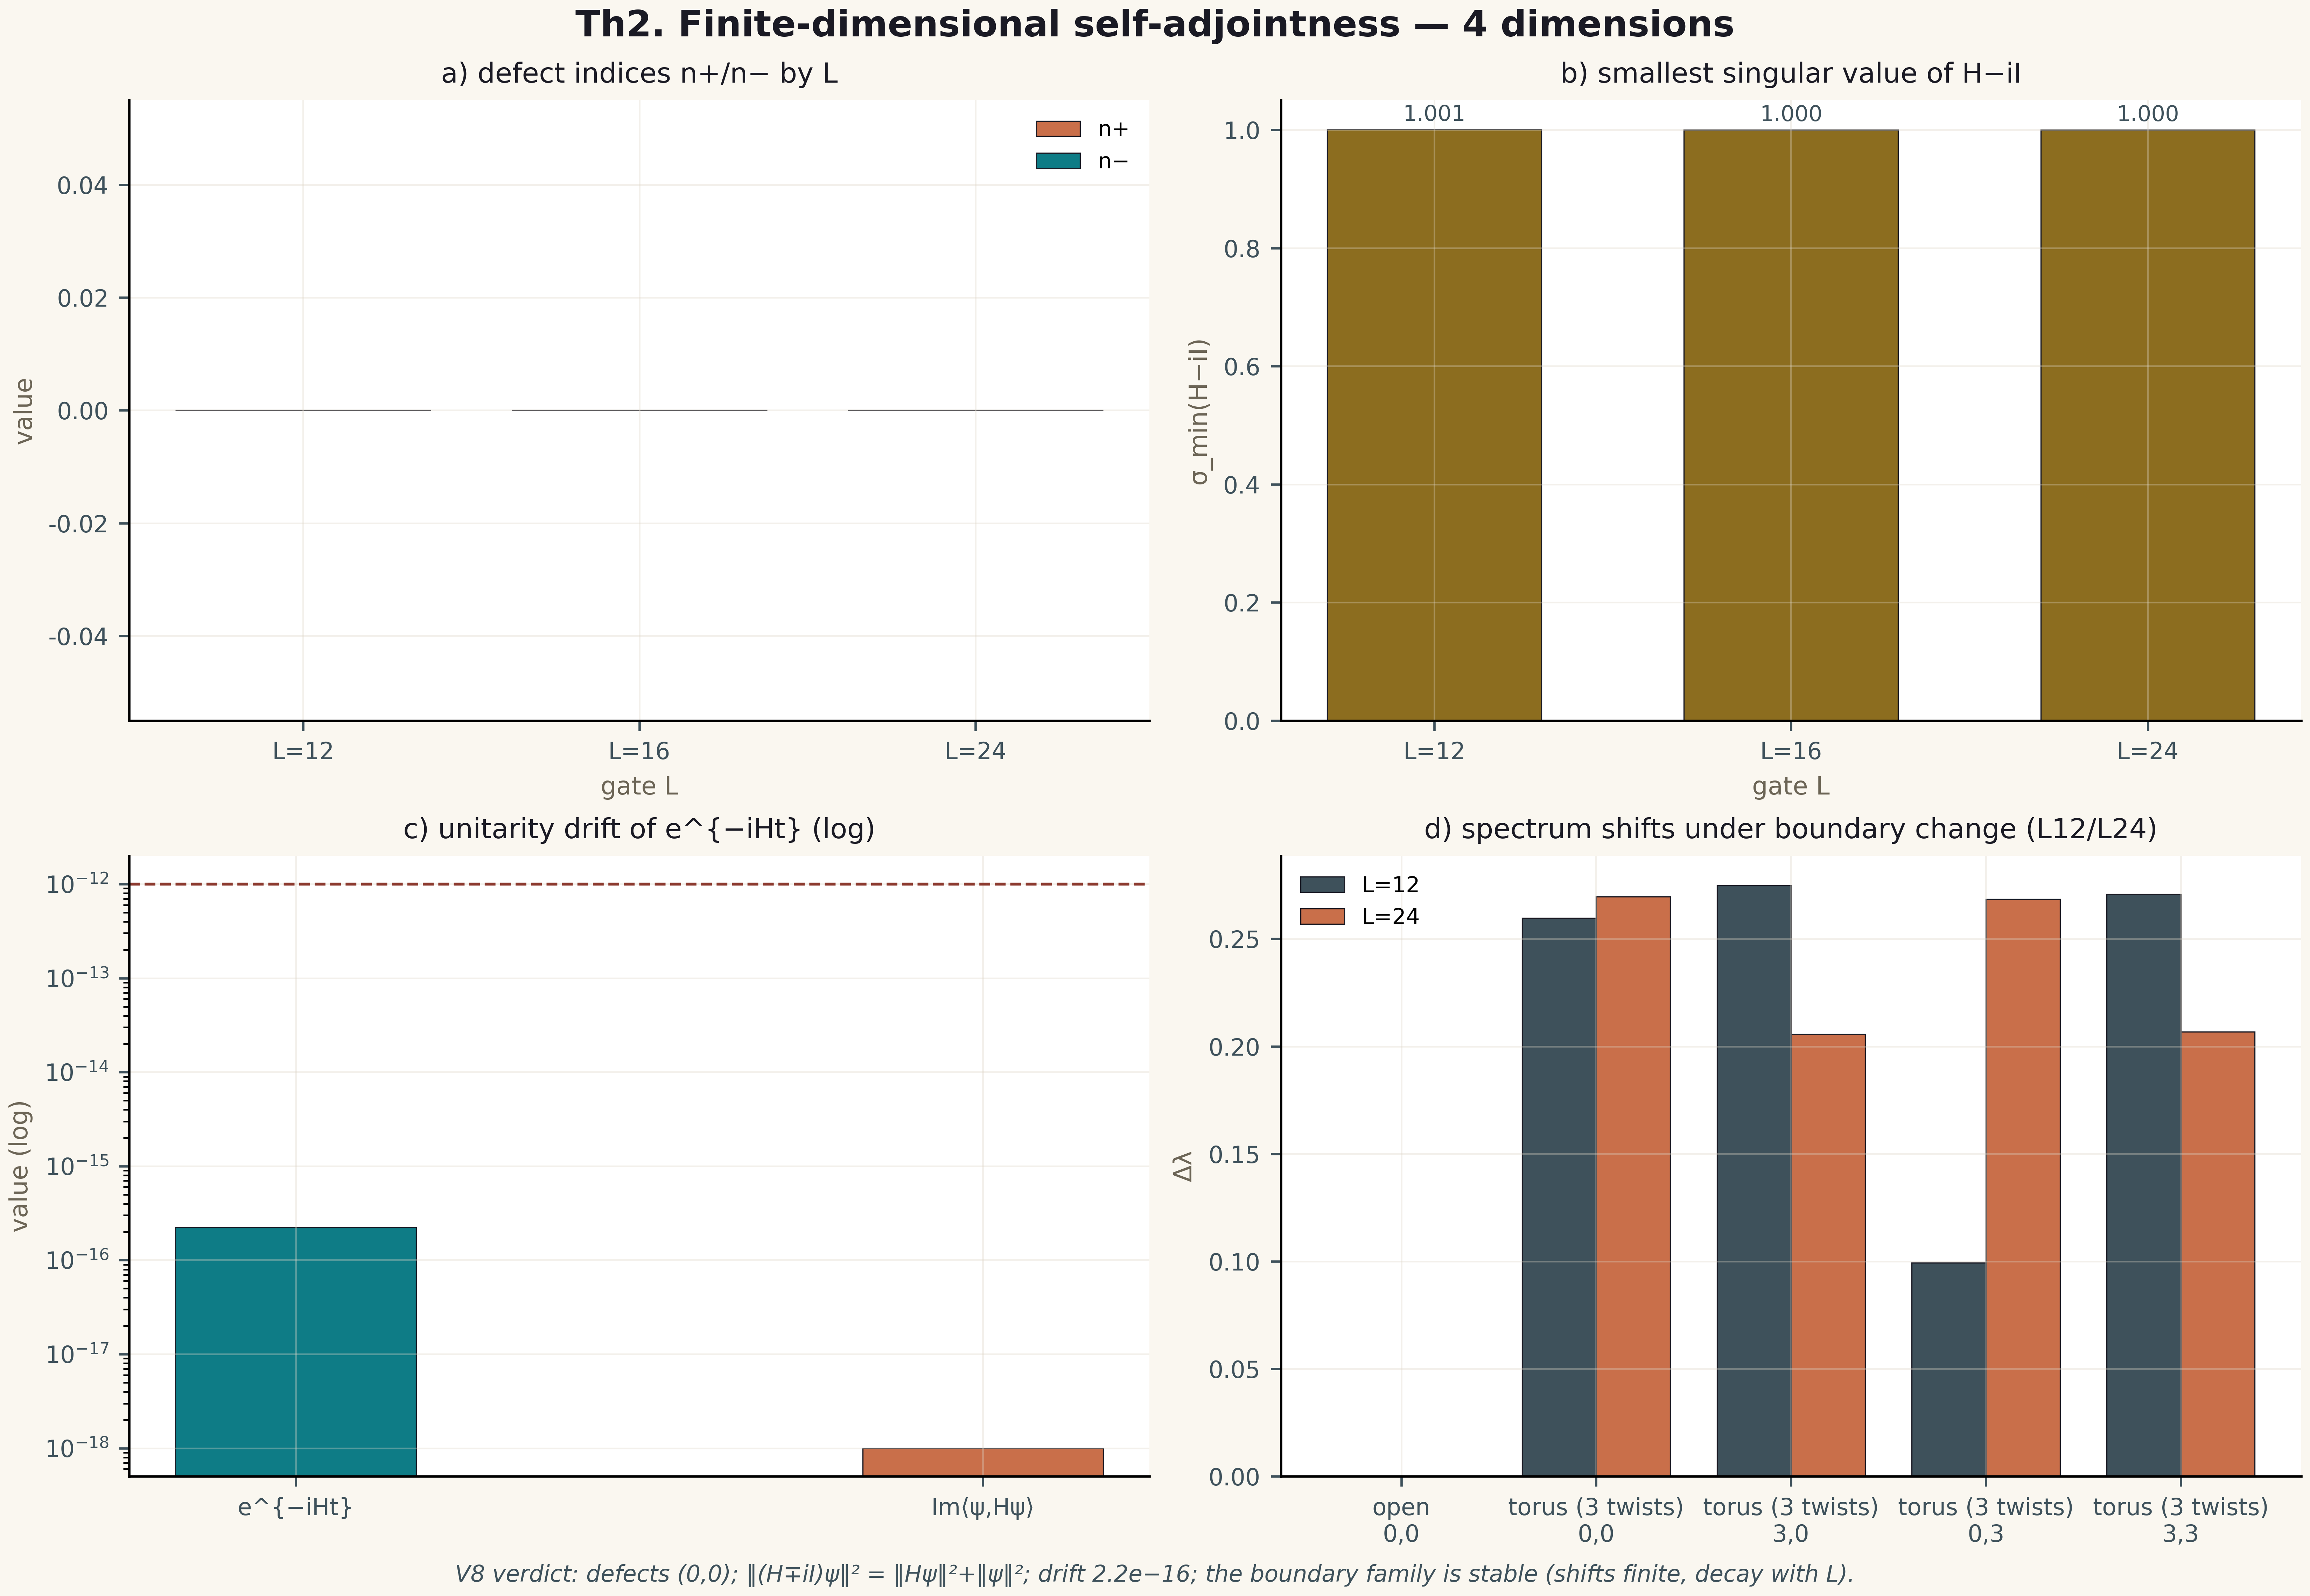
\includegraphics[width=0.9\textwidth,height=105mm,keepaspectratio]{../../../figures_tiled/en/th2_4dim_en.png}
\caption*{Figure 41.1. The Th2 tile: self-adjointness and unitary dynamics (600 dpi).}
\end{figure}

\begin{figure}[htbp]\centering
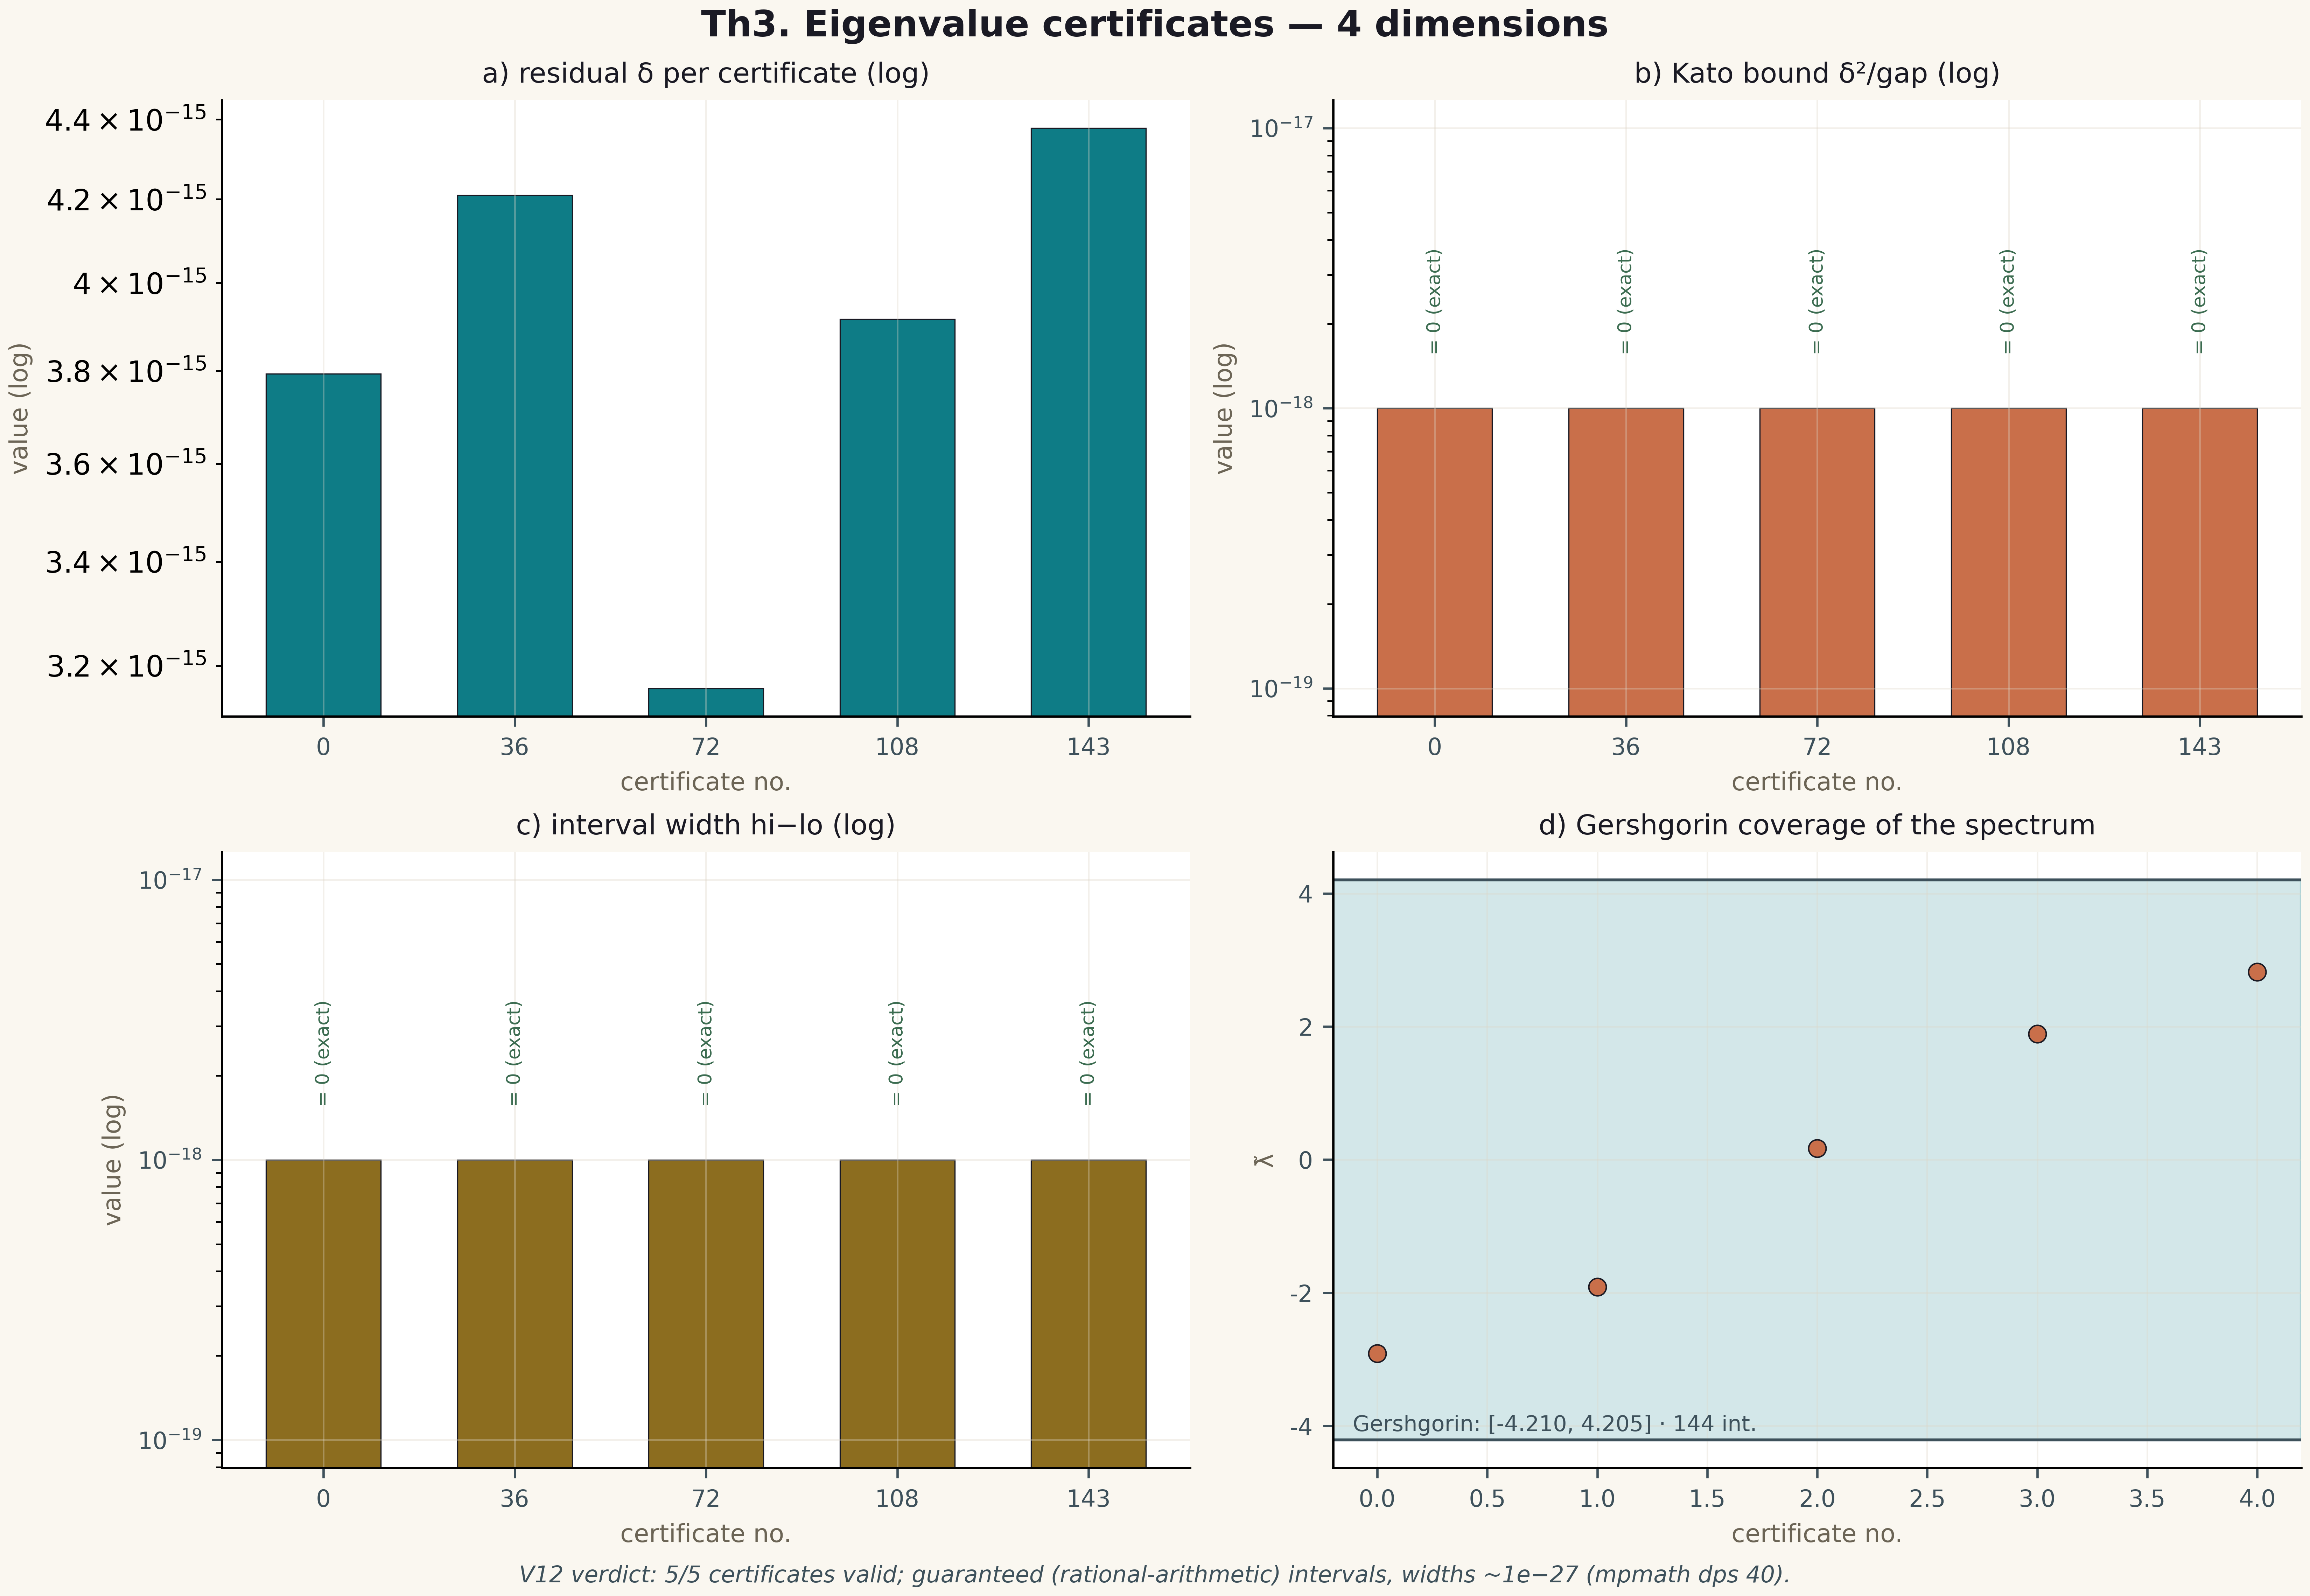
\includegraphics[width=0.9\textwidth,height=105mm,keepaspectratio]{../../../figures_tiled/en/th3_4dim_en.png}
\caption*{Figure 41.2. The Th3 tile: Kato certificates (600 dpi).}
\end{figure}

\begin{figure}[htbp]\centering
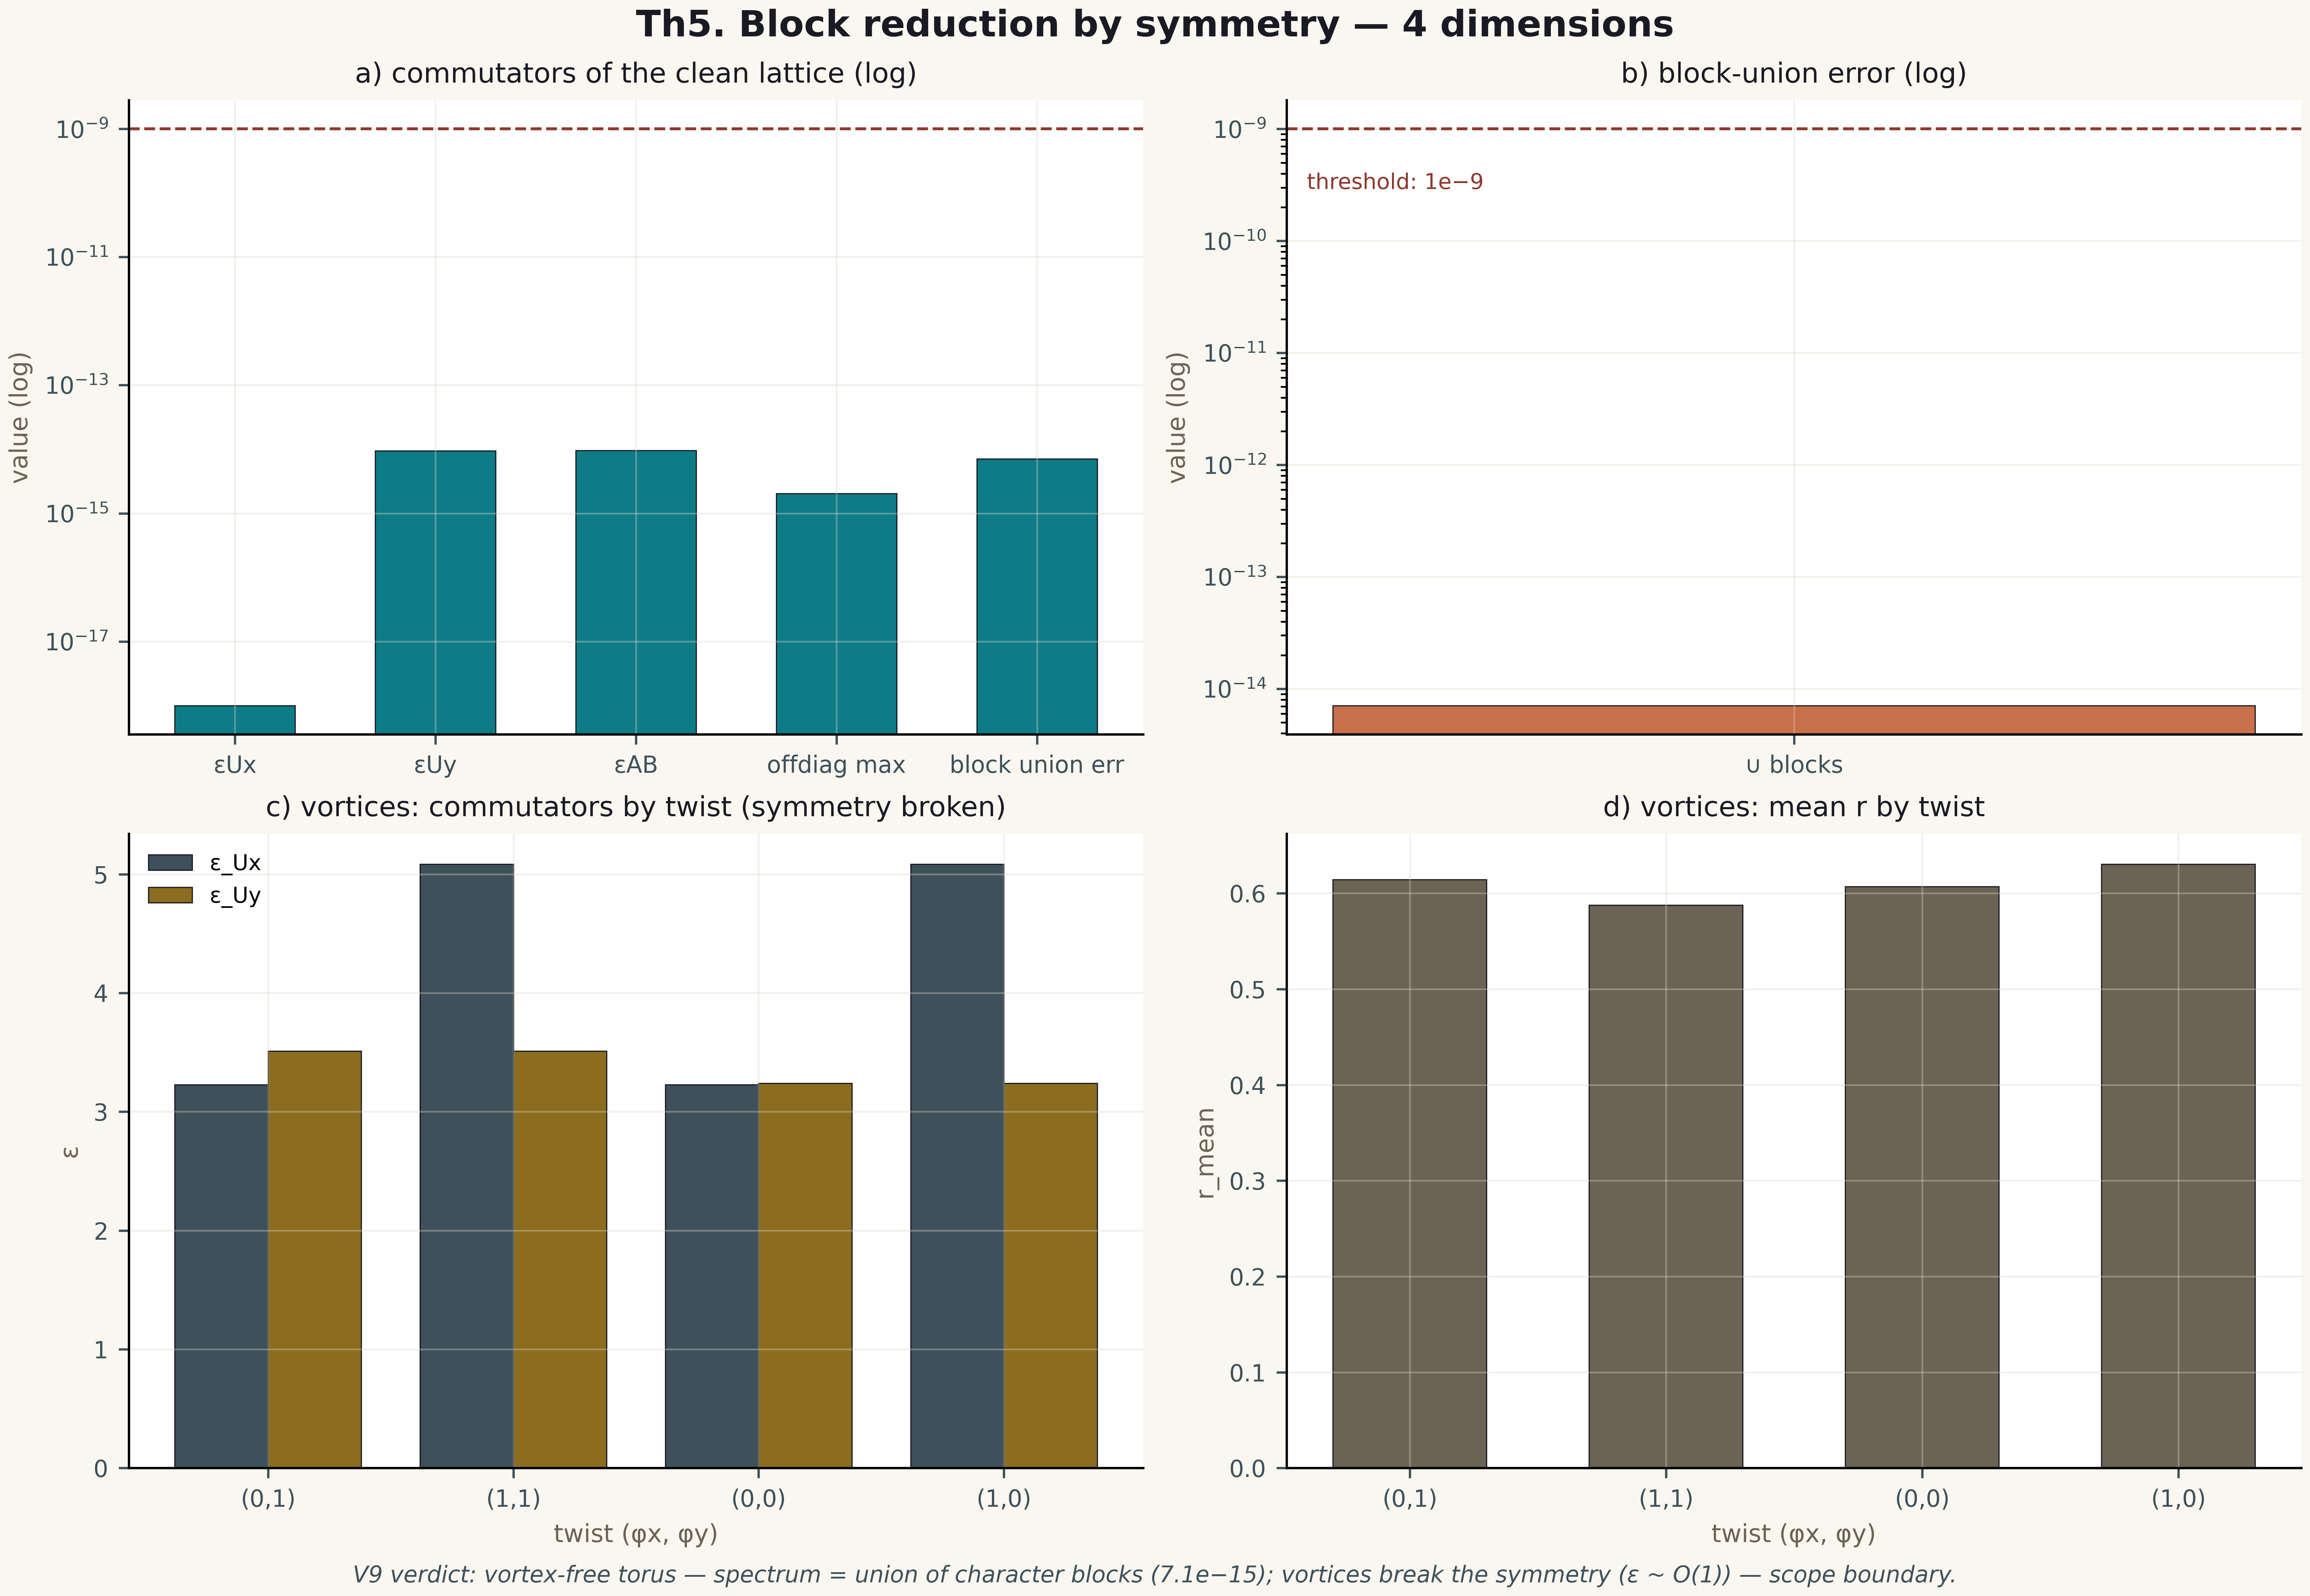
\includegraphics[width=0.9\textwidth,height=105mm,keepaspectratio]{../../../figures_tiled/en/th5_4dim_en.png}
\caption*{Figure 41.3. The Th5 tile: block reduction (600 dpi).}
\end{figure}

\begin{figure}[htbp]\centering
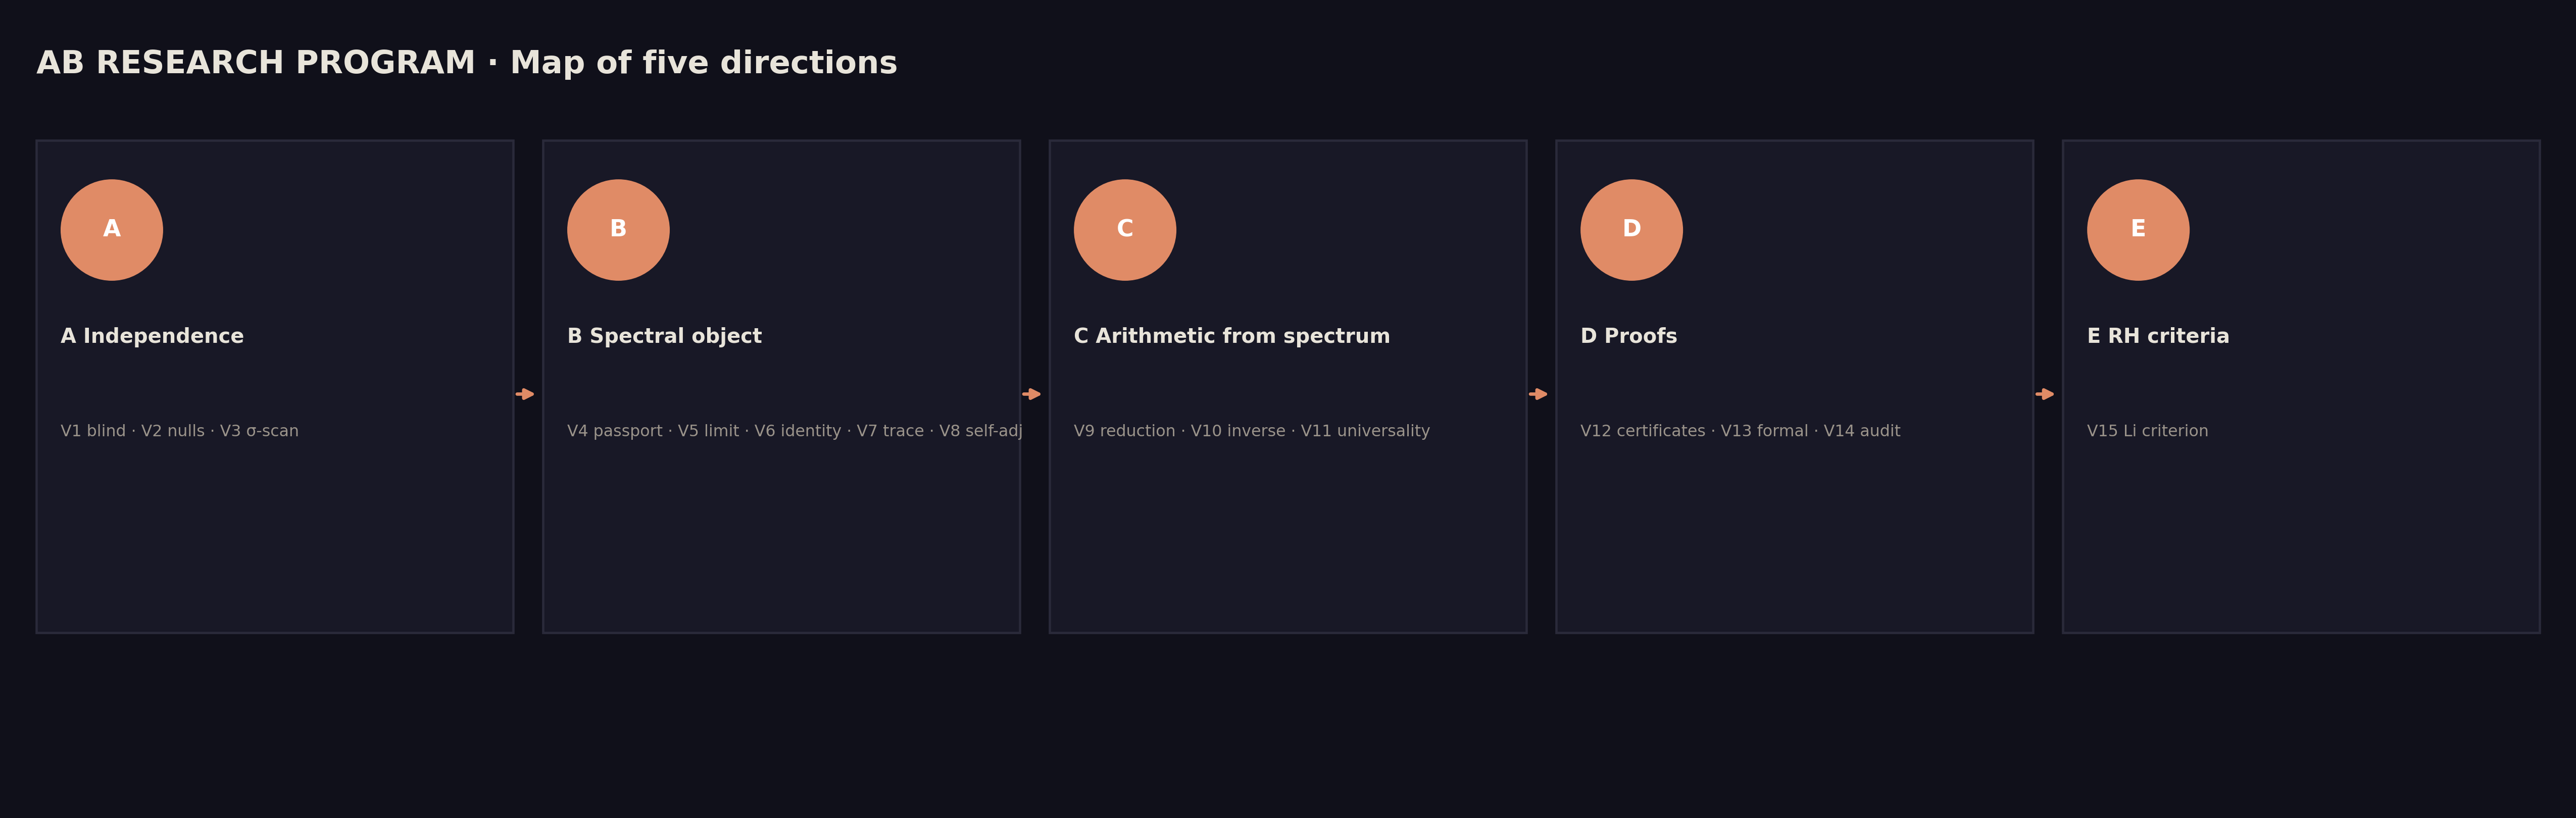
\includegraphics[width=0.9\textwidth,height=105mm,keepaspectratio]{../../../modules/core_spectrum/figures/en/dark/info_map_en.png}
\caption*{Figure 41.4. The core infographic: the spectral level map (dark theme, 600 dpi).}
\end{figure}

\begin{figure}[htbp]\centering
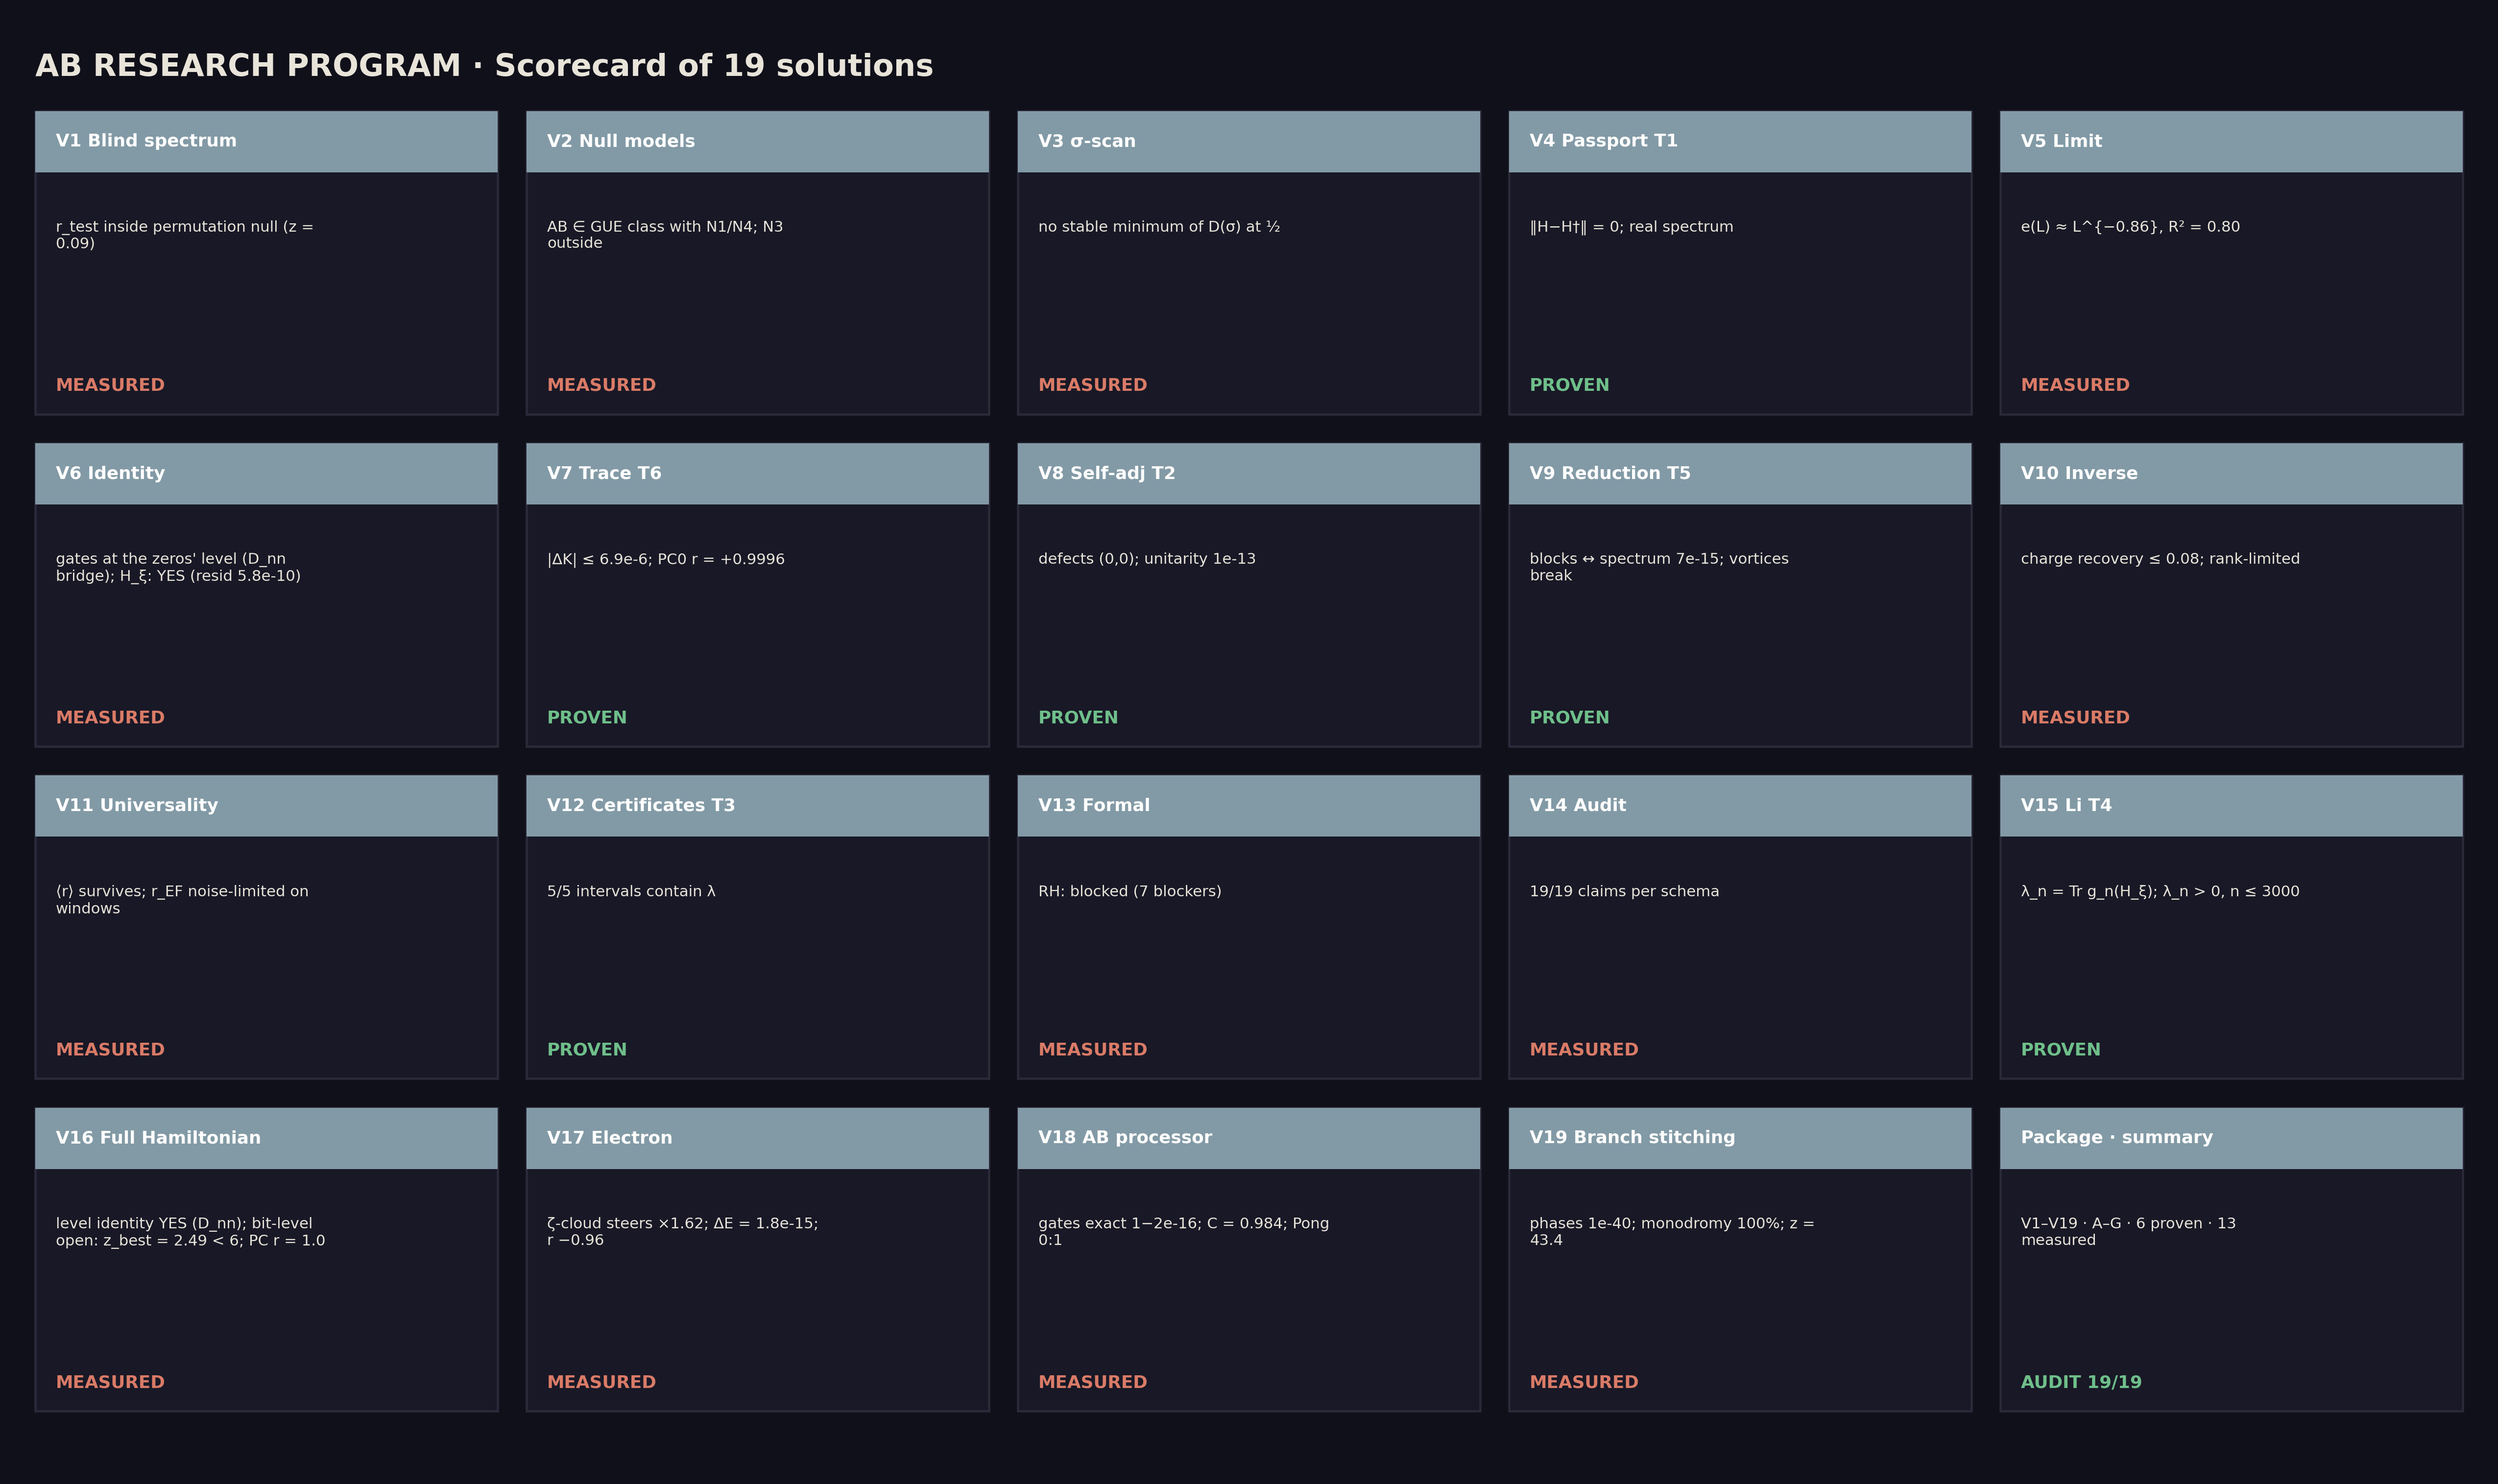
\includegraphics[width=0.9\textwidth,height=105mm,keepaspectratio]{../../../modules/core_spectrum/figures/en/dark/info_scorecard_en.png}
\caption*{Figure 41.5. The core scorecard: the key level certificates (600 dpi).}
\end{figure}

\begin{figure}[htbp]\centering
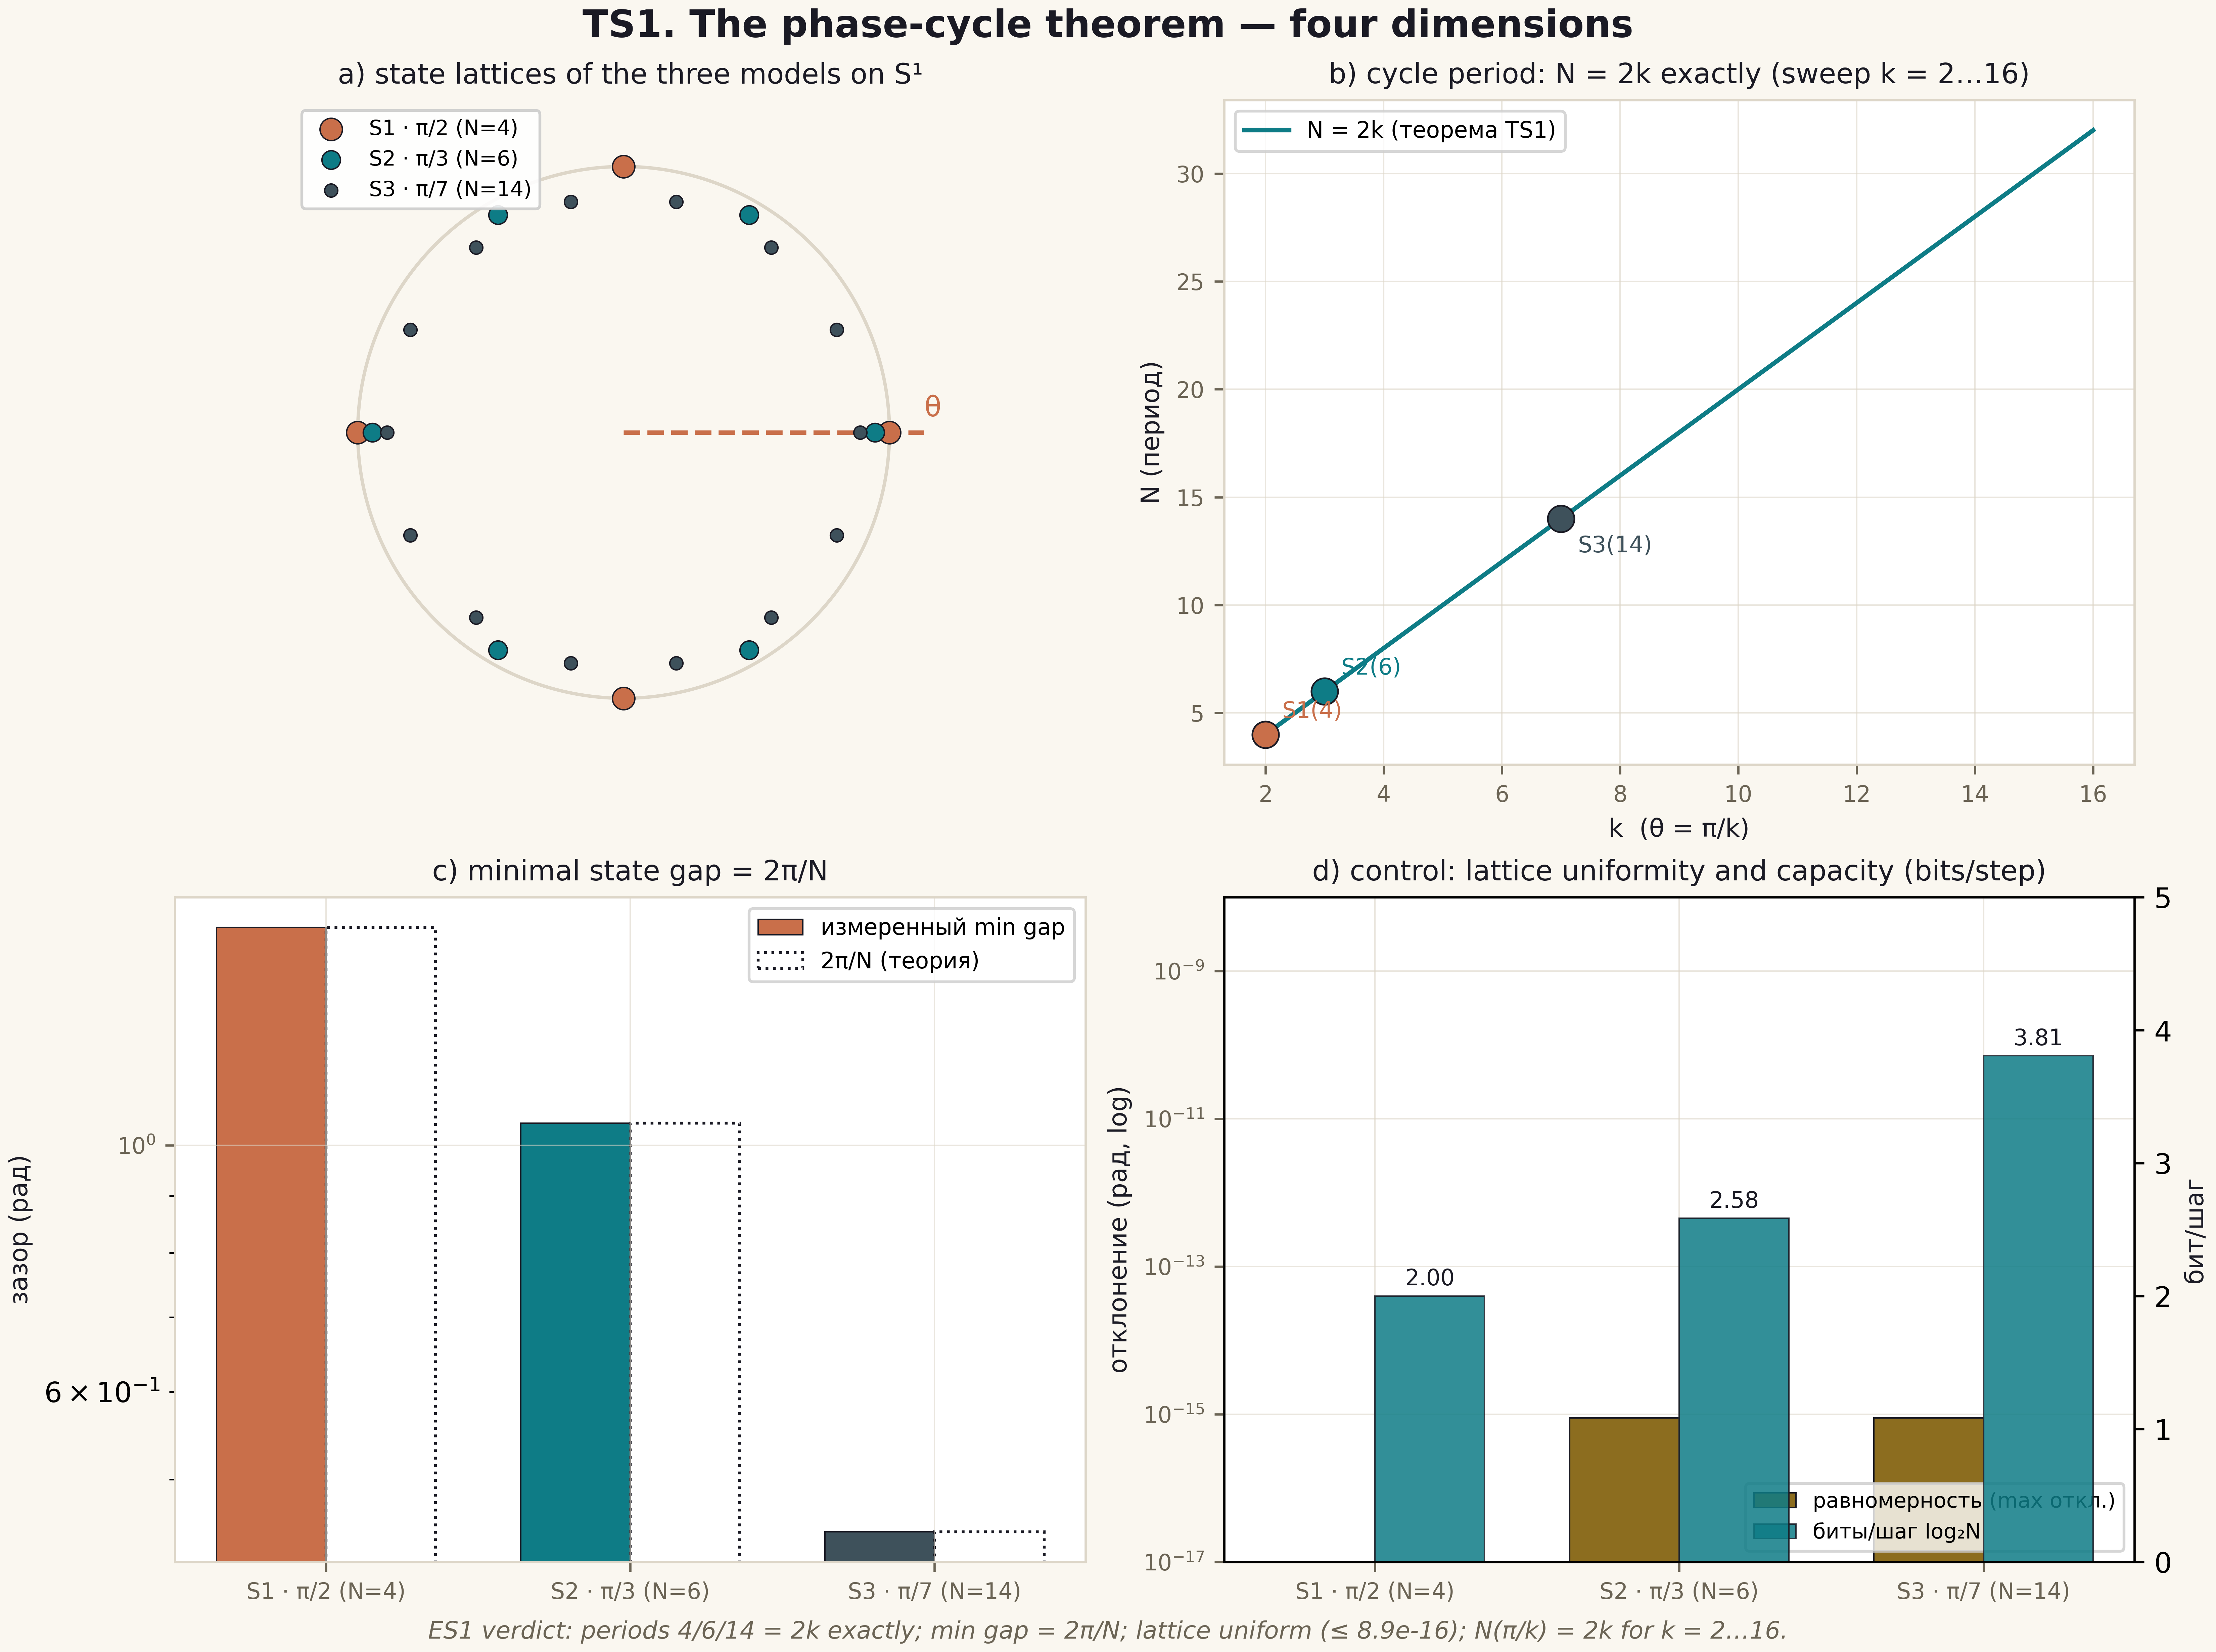
\includegraphics[width=0.9\textwidth,height=105mm,keepaspectratio]{../../../research/realtime_spinor_memory/figures/en/ts1_4dim_en.png}
\caption*{Figure 41.6. The TS1 tile: closure of phase cycles (600 dpi).}
\end{figure}

\begin{figure}[htbp]\centering
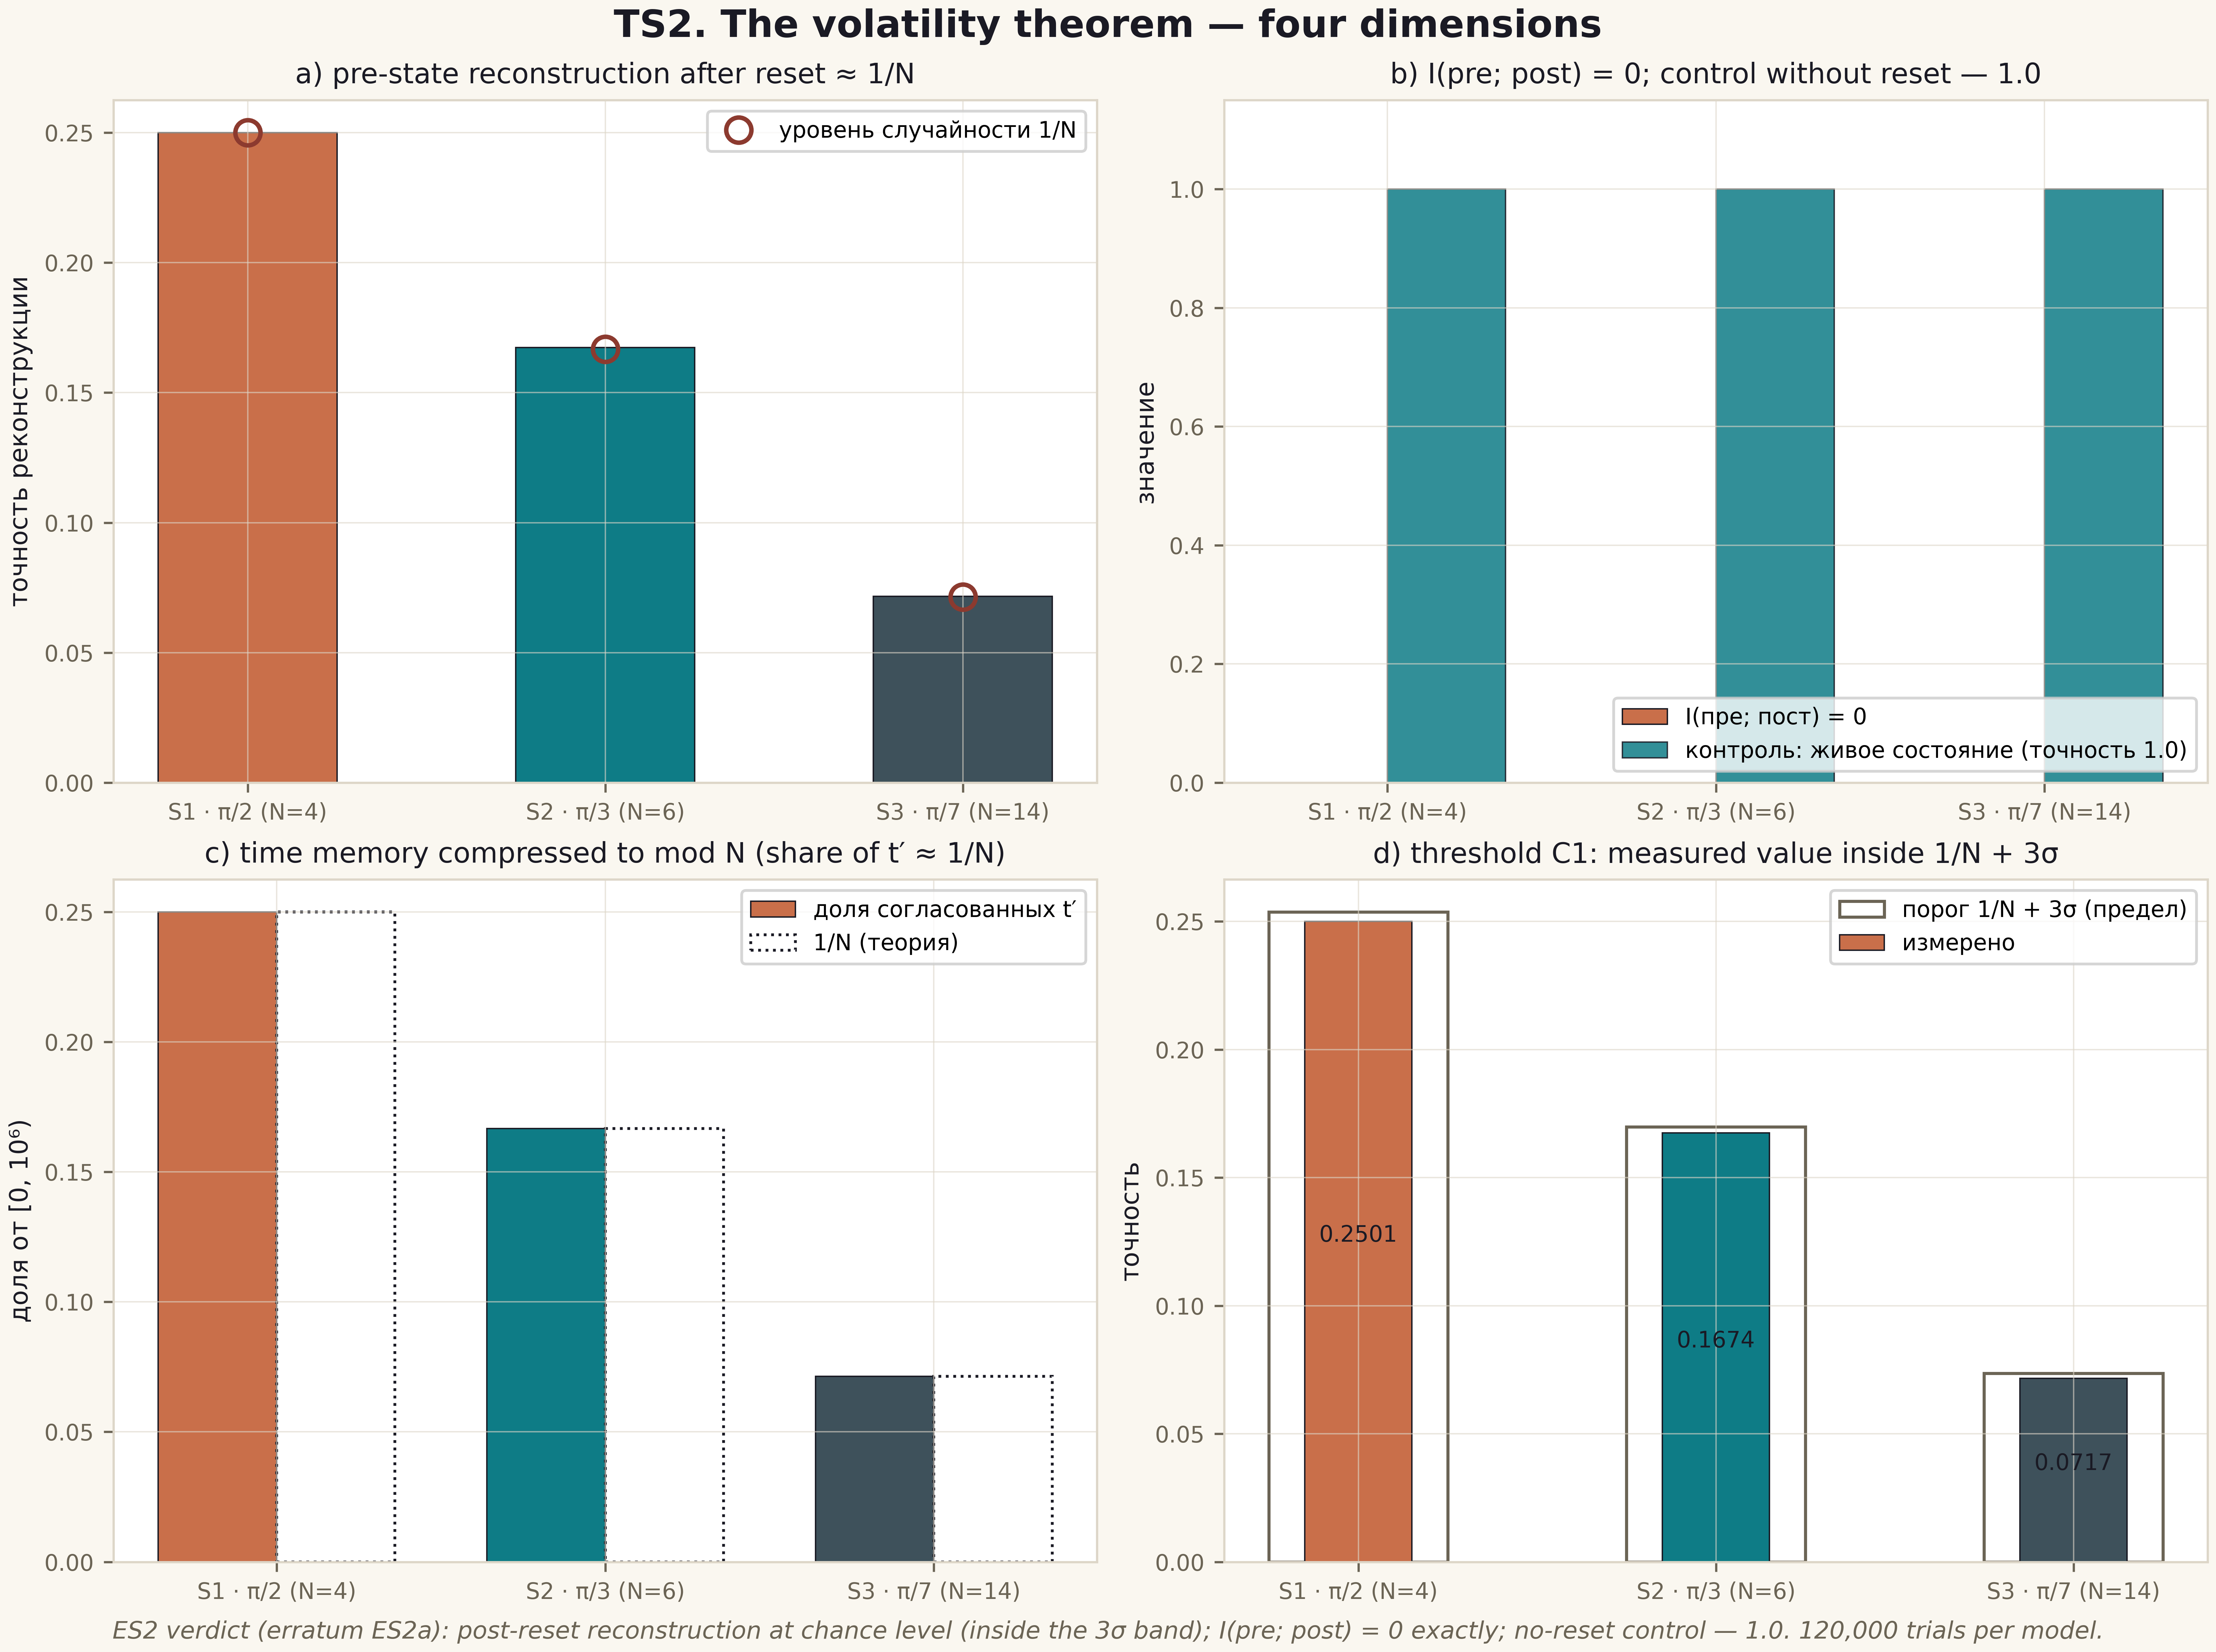
\includegraphics[width=0.9\textwidth,height=105mm,keepaspectratio]{../../../research/realtime_spinor_memory/figures/en/ts2_4dim_en.png}
\caption*{Figure 41.7. The TS2 tile: reset irreversibility (600 dpi).}
\end{figure}

\begin{figure}[htbp]\centering
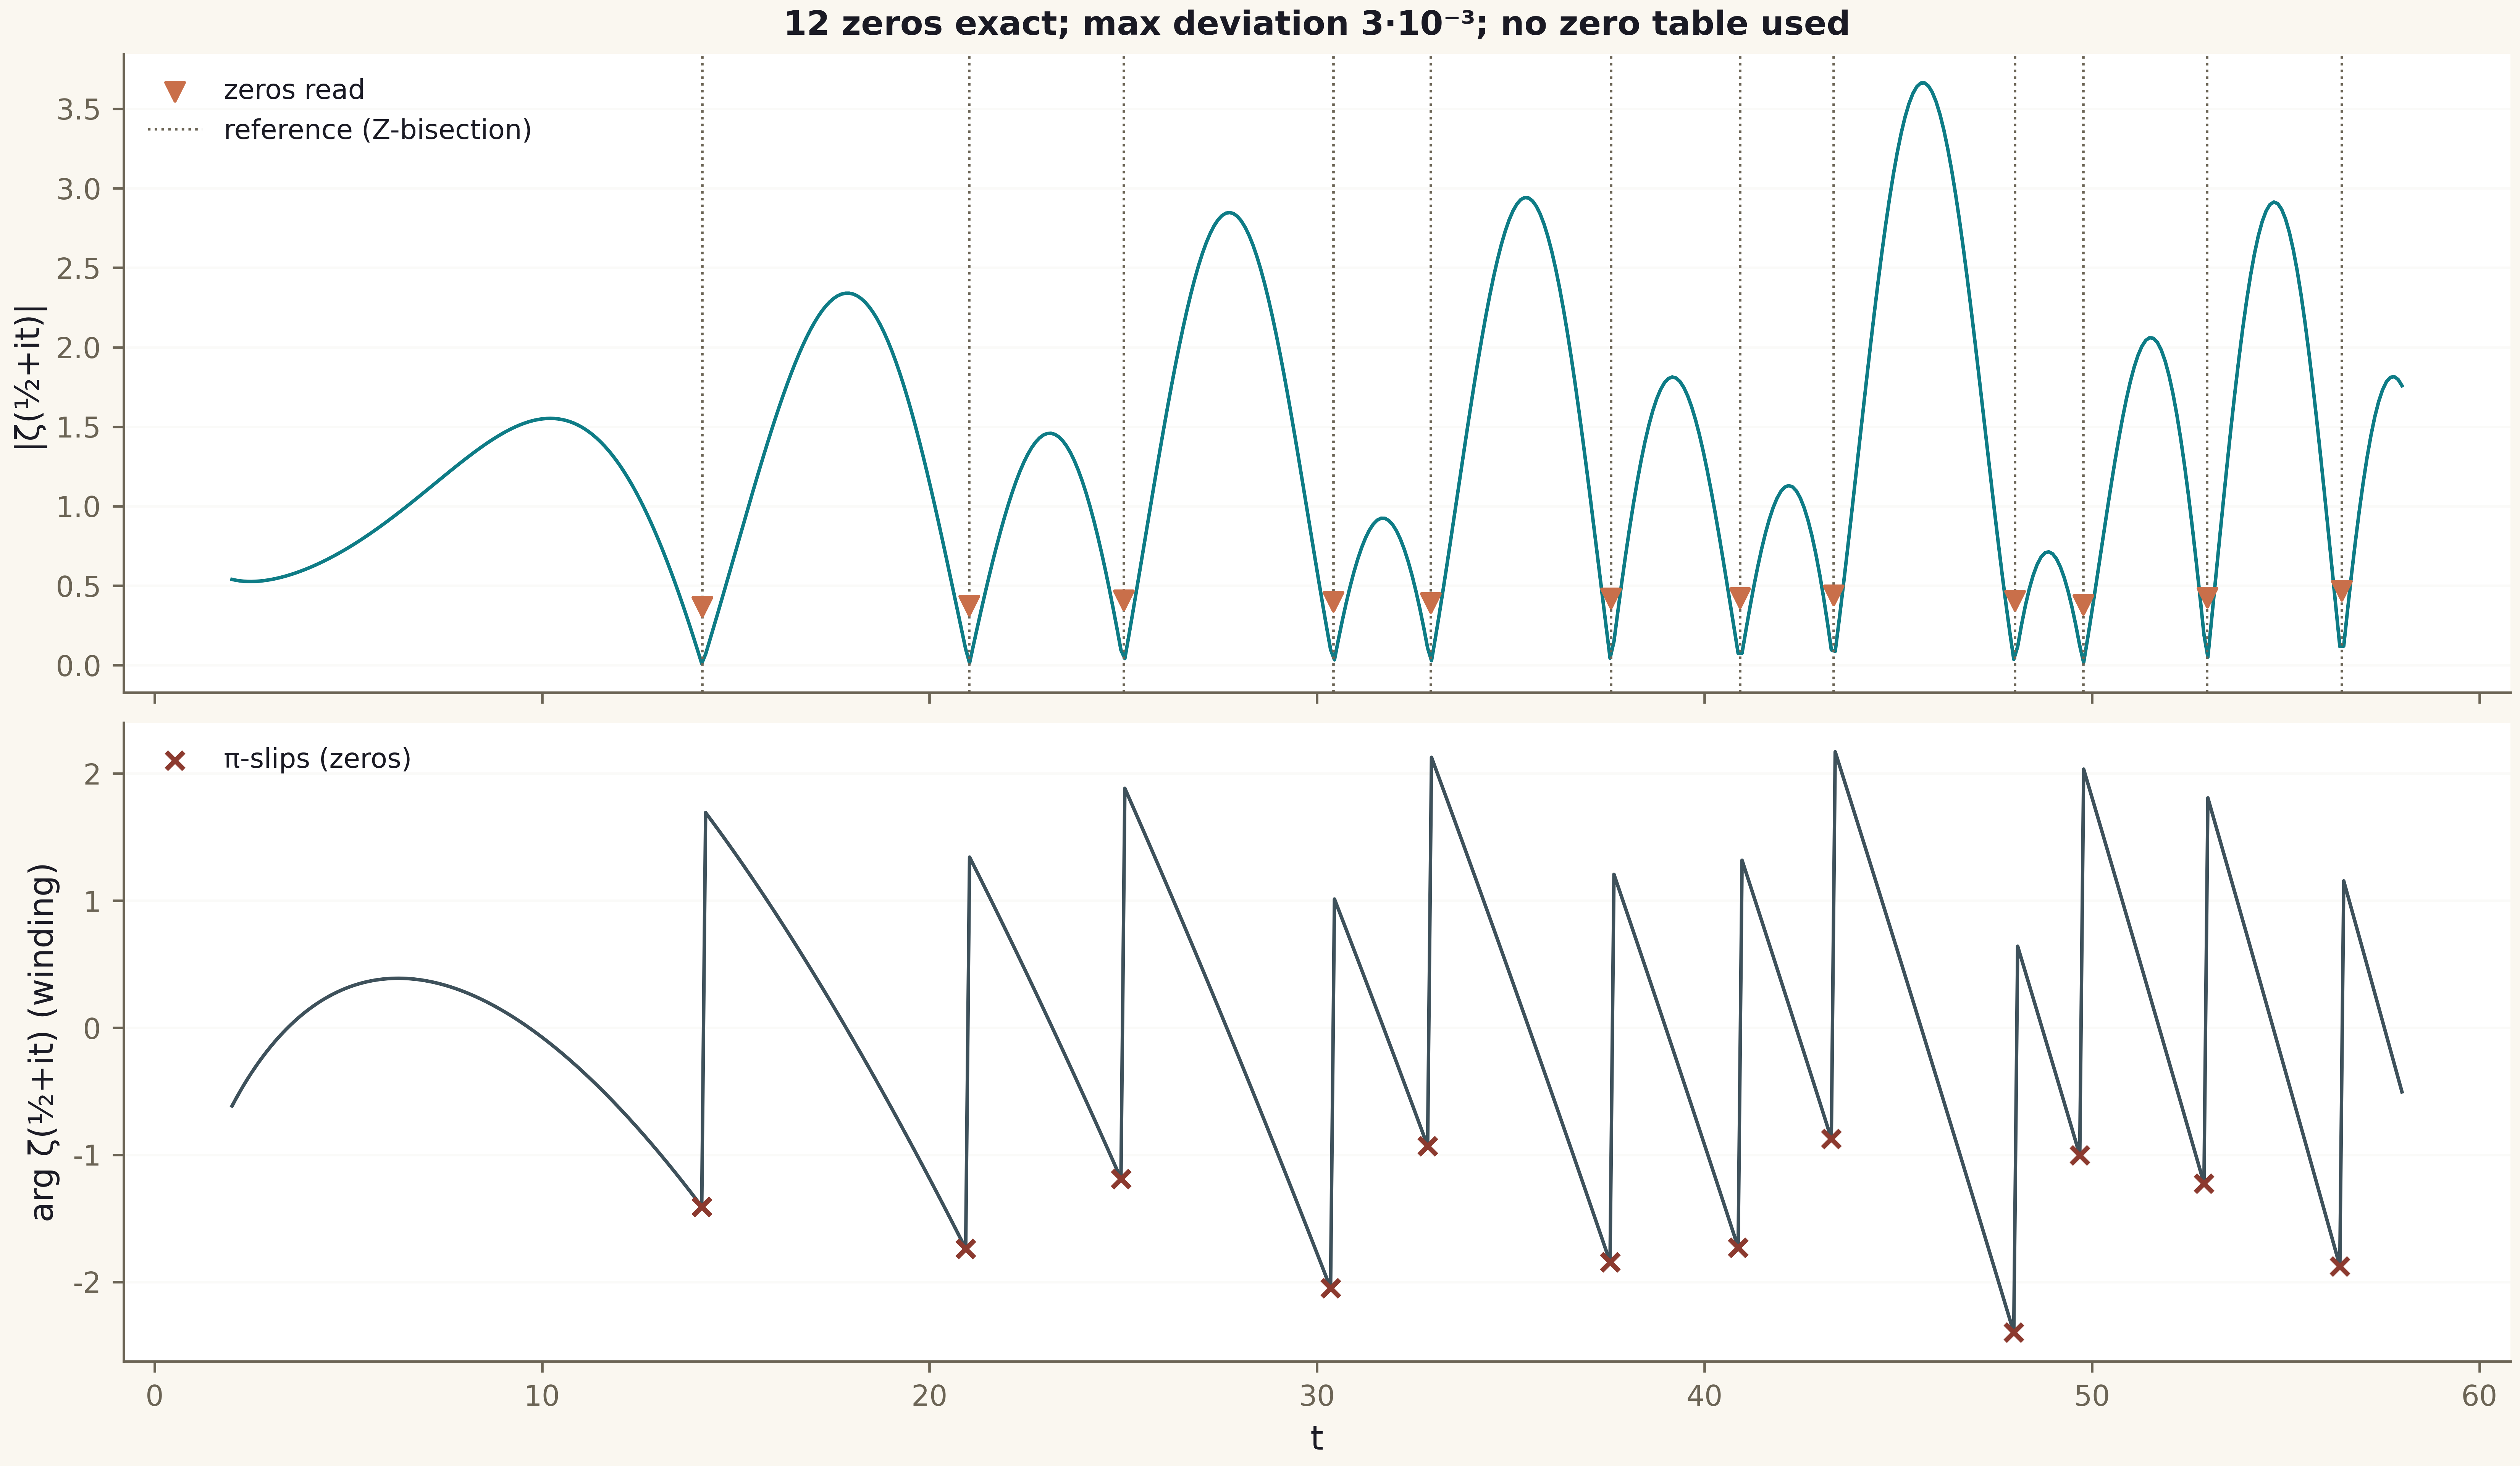
\includegraphics[width=0.9\textwidth,height=105mm,keepaspectratio]{../../../modules/processor_ab/figures_hires/en/fig05_en.png}
\caption*{Figure 41.8. The processor: compilation profiles (600 dpi).}
\end{figure}

\begin{figure}[htbp]\centering
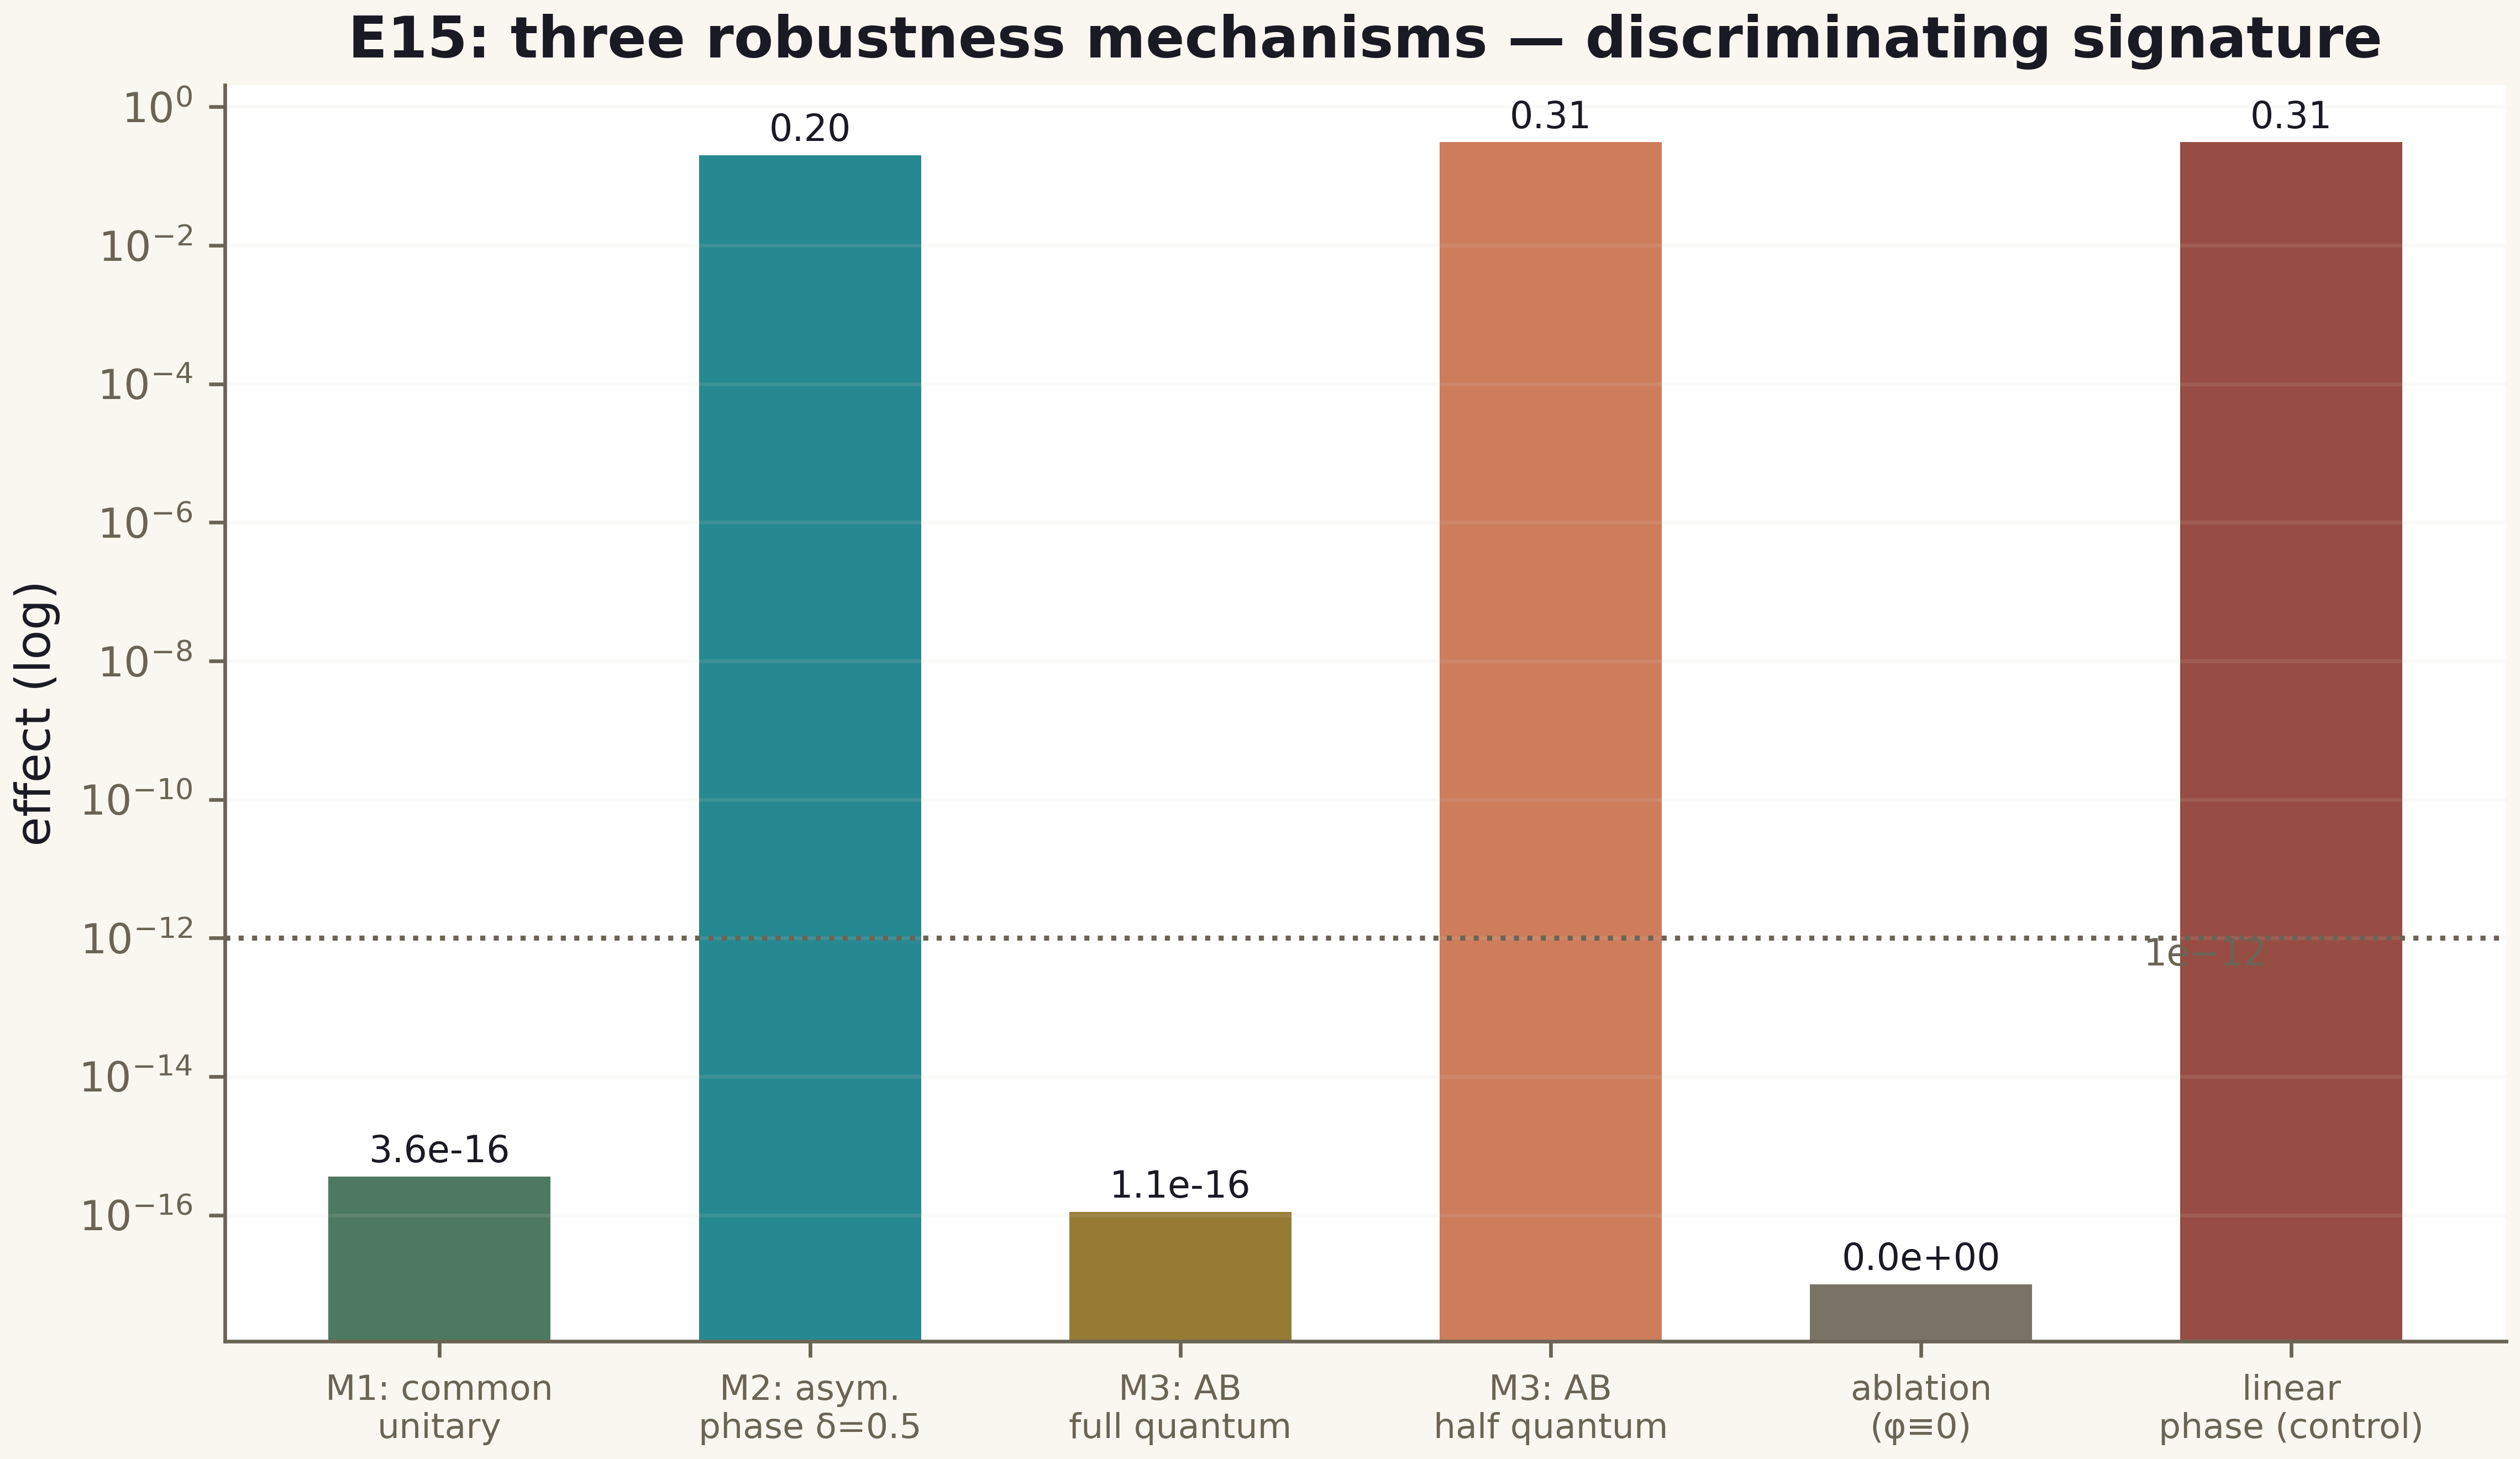
\includegraphics[width=0.9\textwidth,height=105mm,keepaspectratio]{../../../modules/verifier_multilang/figures_hires/en/fig08_en.png}
\caption*{Figure 41.9. Verification: the step cost (600 dpi).}
\end{figure}

\section{Chapter 42. The Limits of the Method: What the Program Cannot Do}

\noindent\textit{\color{copper}An honest monograph must describe not only achievements but the limits of the method. This chapter systematizes the limitations — fundamental, technical and disciplinary — and explains which are surmountable and by which routes.}

\subsection{42.1. Fundamental limitations}

\begin{itemize}
  \item \textbf{RH is not proved and will not be proved numerically.} Neither the volume of data, nor the accuracy, nor the beauty of the agreement substitutes the analytic proof of the four hypotheses of the V13 machine. This is not a failure of the method but its definition.
  \item \textbf{Statistics ≠ arithmetic.} Any GUE agreement is reproducible by random models; the specificity lives in the fine structure (the trace, the constants), and its measurement is the only honest path.
  \item \textbf{The Markov class of tasks.} The memoryless machine solves tasks admitting a Markov policy; tasks with substantial history require memory — and then the architecture applies other levels, not the spinor models.
  \item \textbf{The human factor of protocols.} Blindness protects against leaks, not against an error in the protocol itself; the γ₁₂ erratum showed that the framework must be checked too.
\end{itemize}

\subsection{42.2. Technical limitations}

\begin{itemize}
  \item \textbf{Heights T.} The flagships reach T = 1000; T ≫ 1000 is the O-J5 target, requiring a new computational wave.
  \item \textbf{Compilation sizes.} V20 is certified for 4×4 and 8×8; larger sizes are a matter of arithmetic and depth, fixed in the roadmap.
  \item \textbf{The ISA class.} The KAK optimum is unreachable in the class; extending the class is a separate decision with its own verdicts.
  \item \textbf{The idealization of reset.} TS2 speaks of an ideal reset; real channels add a contribution measured by ES5.
\end{itemize}

\subsection{42.3. Disciplinary limitations}

The program deliberately pays for honesty with speed: pre-registration is slower than "free search", blind protocols are more expensive than direct comparisons, statuses require formalization. This is a price the program considers justified: a result obtained without these constraints would have to be re-verified in full. The limits of the method are not a flaw of the program but its interface: they tell a partner which obligations can be relied upon.

\begin{table}[htbp]\centering\small
\caption{Table 42.1. Limitations and routes past them}
\begin{tabular}{p{0.29\textwidth} p{0.17\textwidth} p{0.50\textwidth}}
\toprule
\textbf{Limitation} & \textbf{Type} & \textbf{Route}
\midrule
RH blocked & fundamental & analytic proofs of O08/O09/O11/O12 \\
GUE insufficiency & fundamental & fine structure: trace, constants, behaviour \\
T = 1000 & technical & O-J5: a new computational wave \\
4×4/8×8 & technical & extending the arithmetic and depth (P5) \\
KAK outside the class & class-level & extending the ISA with new verdicts \\
ideal reset & model-level & ES5: measuring real channels \\
\bottomrule
\end{tabular}
\end{table}

\section{Chapter 43. The Level Figures Gallery}

\noindent\textit{\color{copper}Selected figures of the core, processor and verification levels (EN versions, 600 dpi; RU — in figures\_hires/ru/). All figures are built from committed verdicts.}

\begin{figure}[htbp]\centering
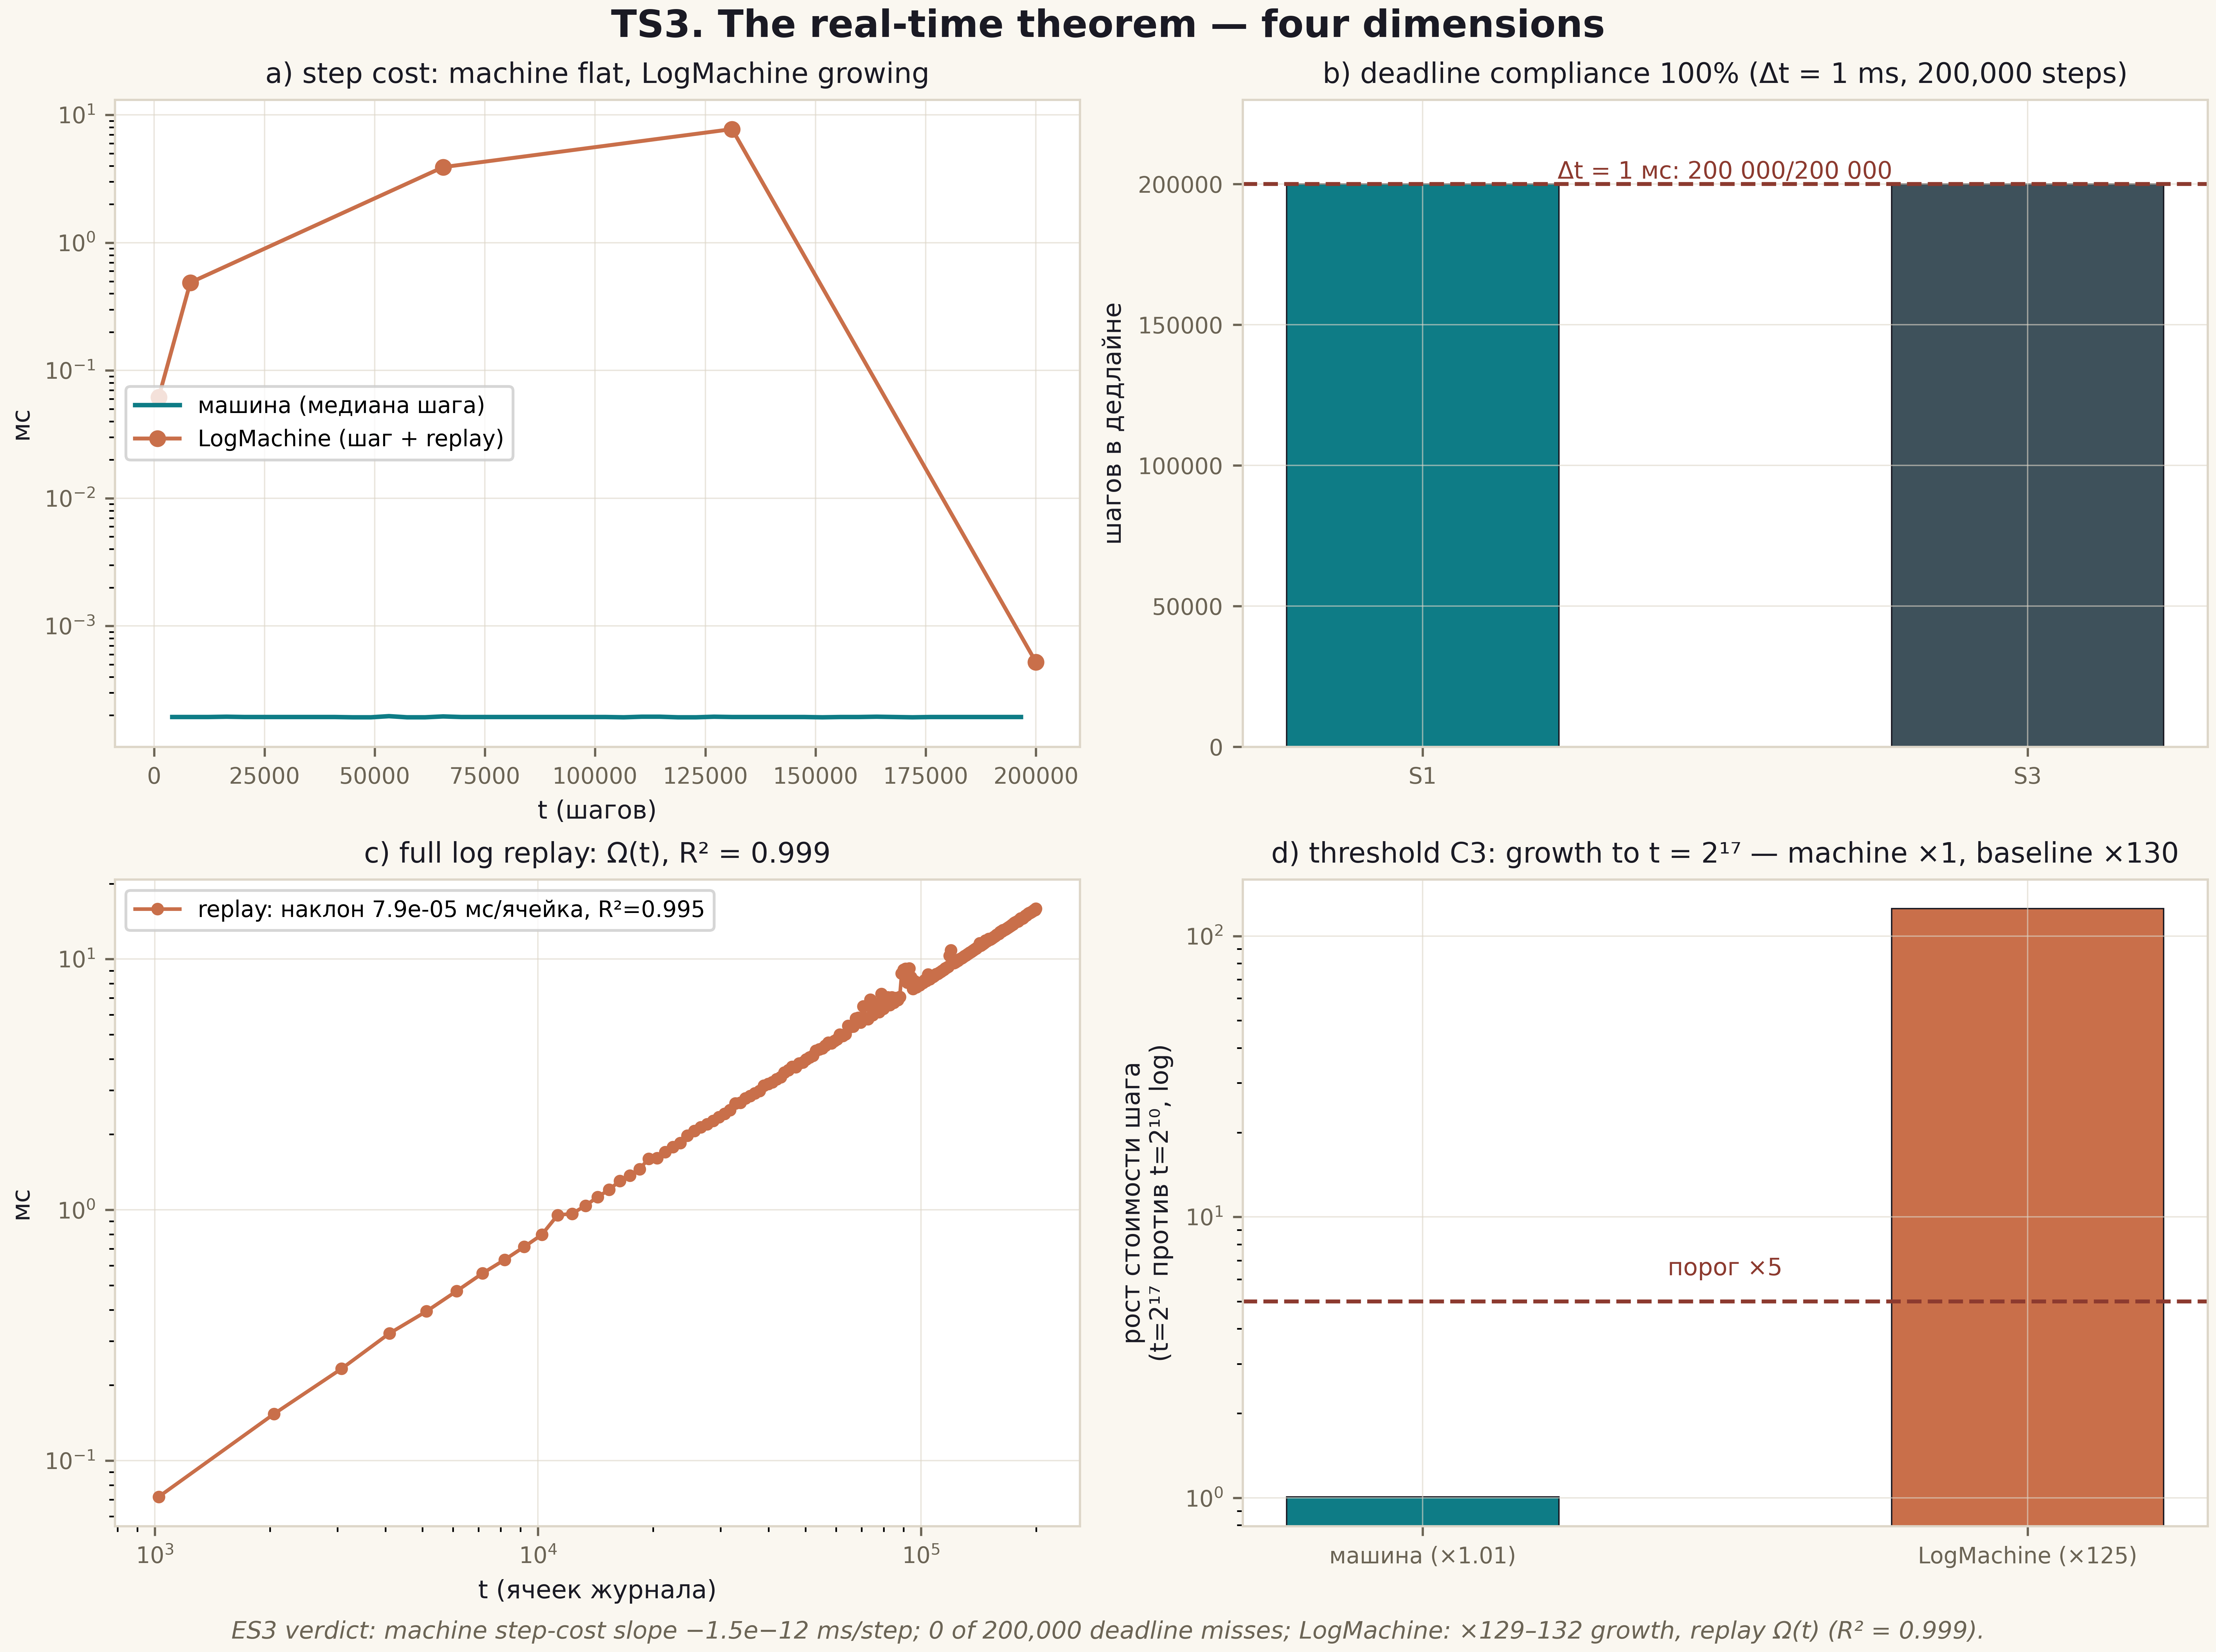
\includegraphics[width=0.9\textwidth,height=105mm,keepaspectratio]{../../../research/realtime_spinor_memory/figures/en/ts3_4dim_en.png}
\caption*{Figure 43.1. The TS3 tile: O(1) steps against the Ω(t) log (600 dpi).}
\end{figure}

\begin{figure}[htbp]\centering
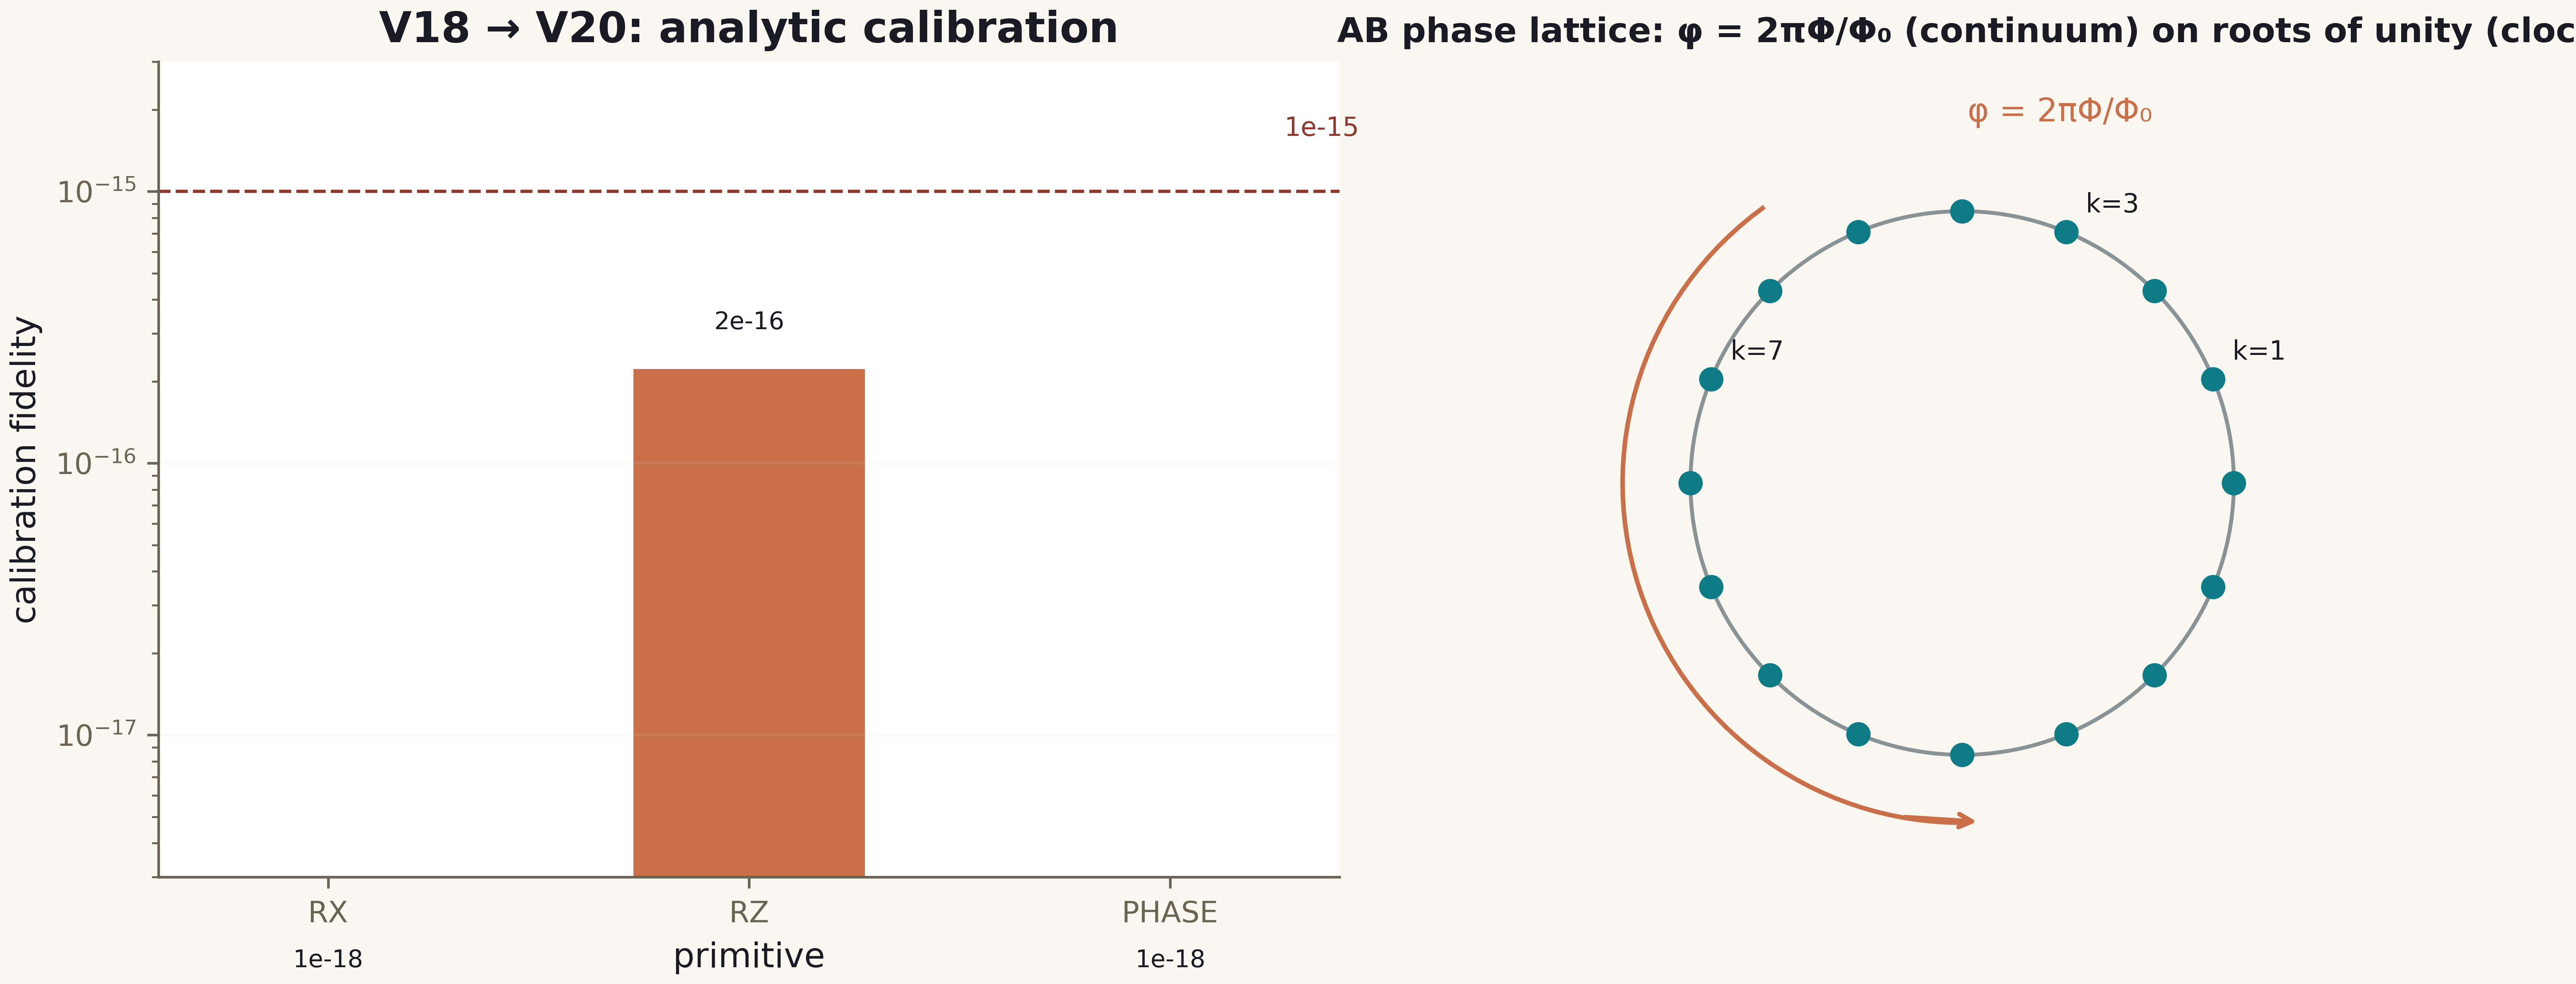
\includegraphics[width=0.9\textwidth,height=105mm,keepaspectratio]{../../../modules/processor_ab/figures_hires/en/fig01_en.png}
\caption*{Figure 43.2. The processor: compilation accuracy by target (600 dpi).}
\end{figure}

\begin{figure}[htbp]\centering
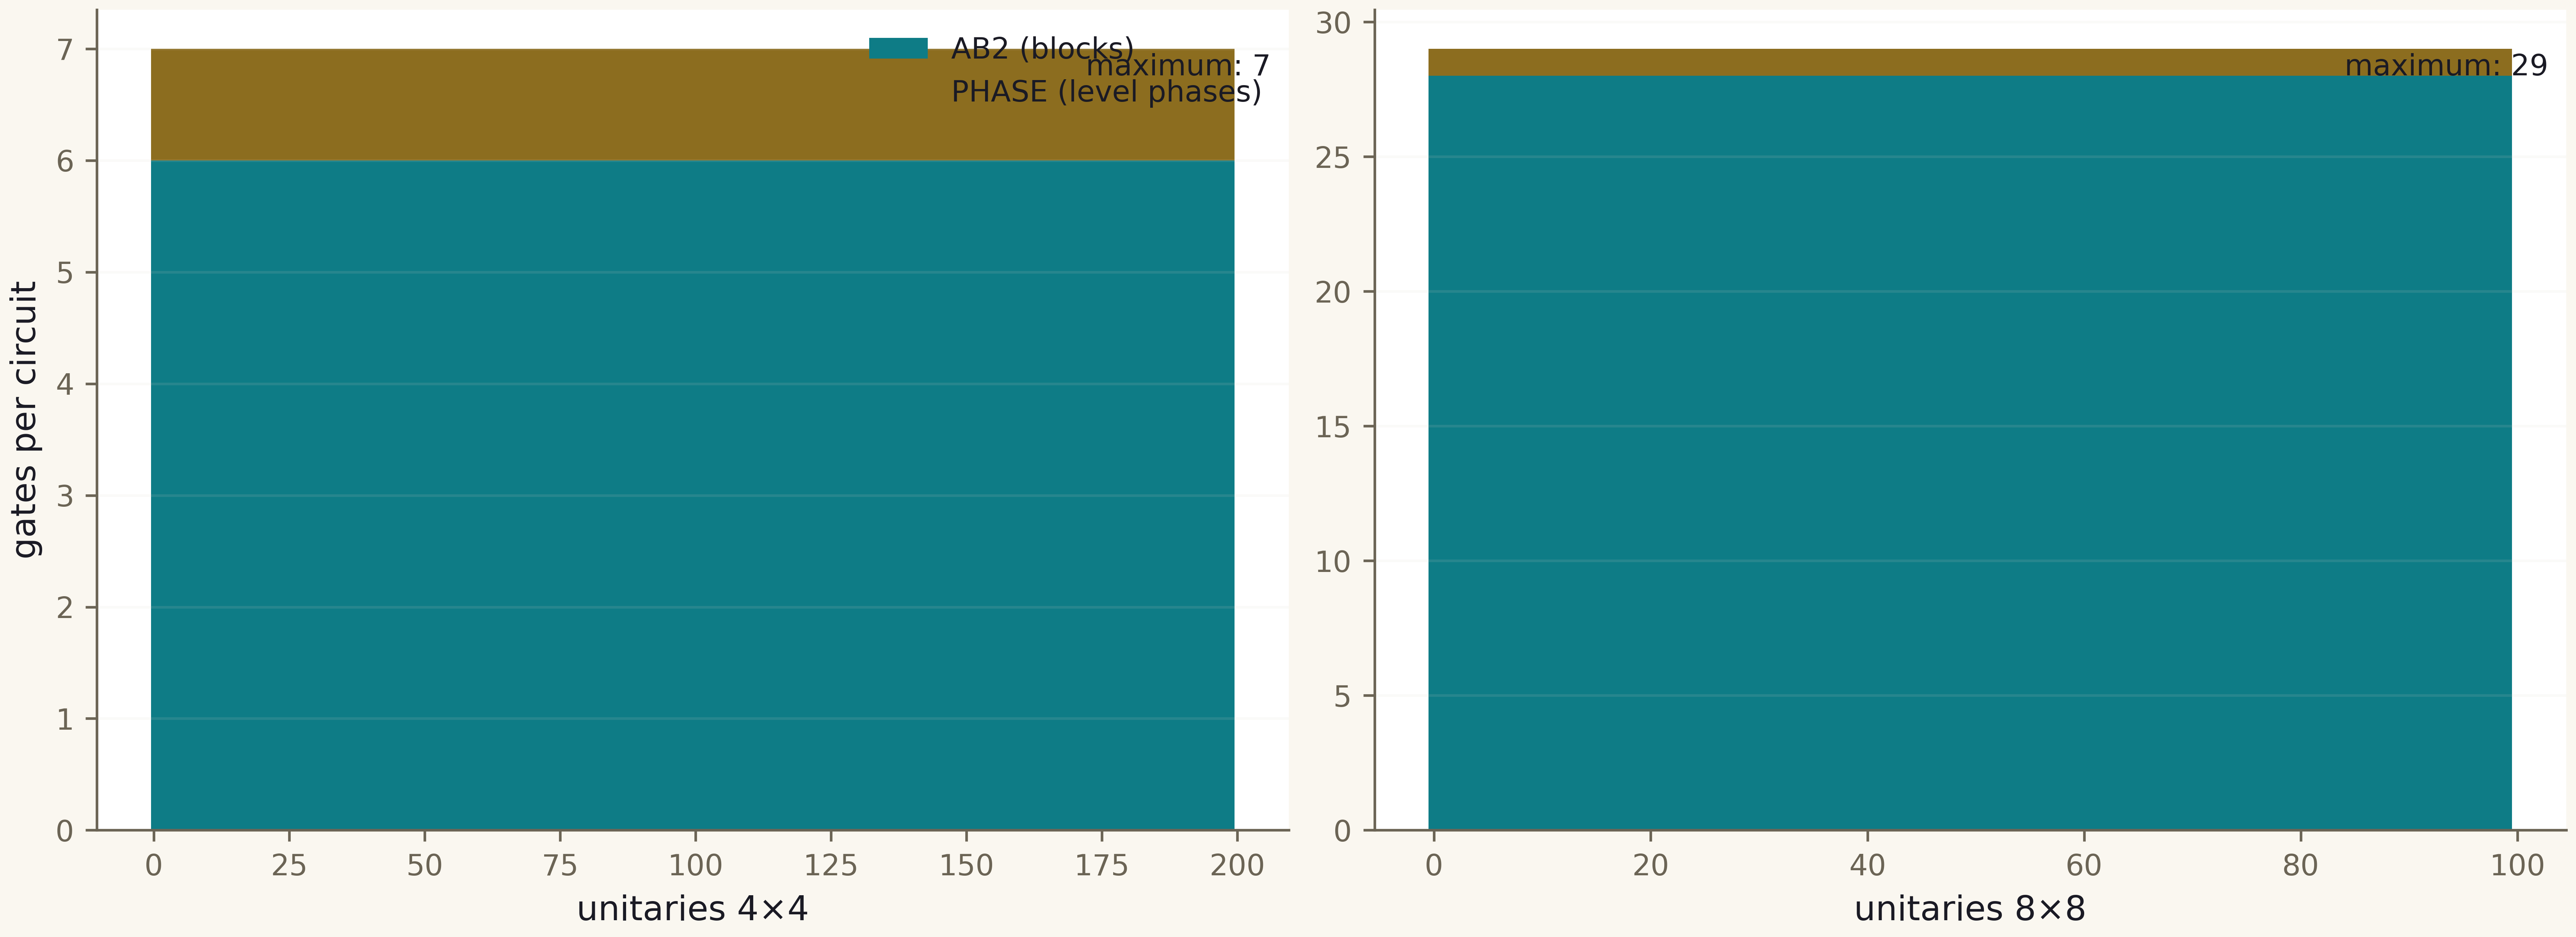
\includegraphics[width=0.9\textwidth,height=105mm,keepaspectratio]{../../../modules/processor_ab/figures_hires/en/fig03_en.png}
\caption*{Figure 43.3. The processor: gate depths (600 dpi).}
\end{figure}

\begin{figure}[htbp]\centering
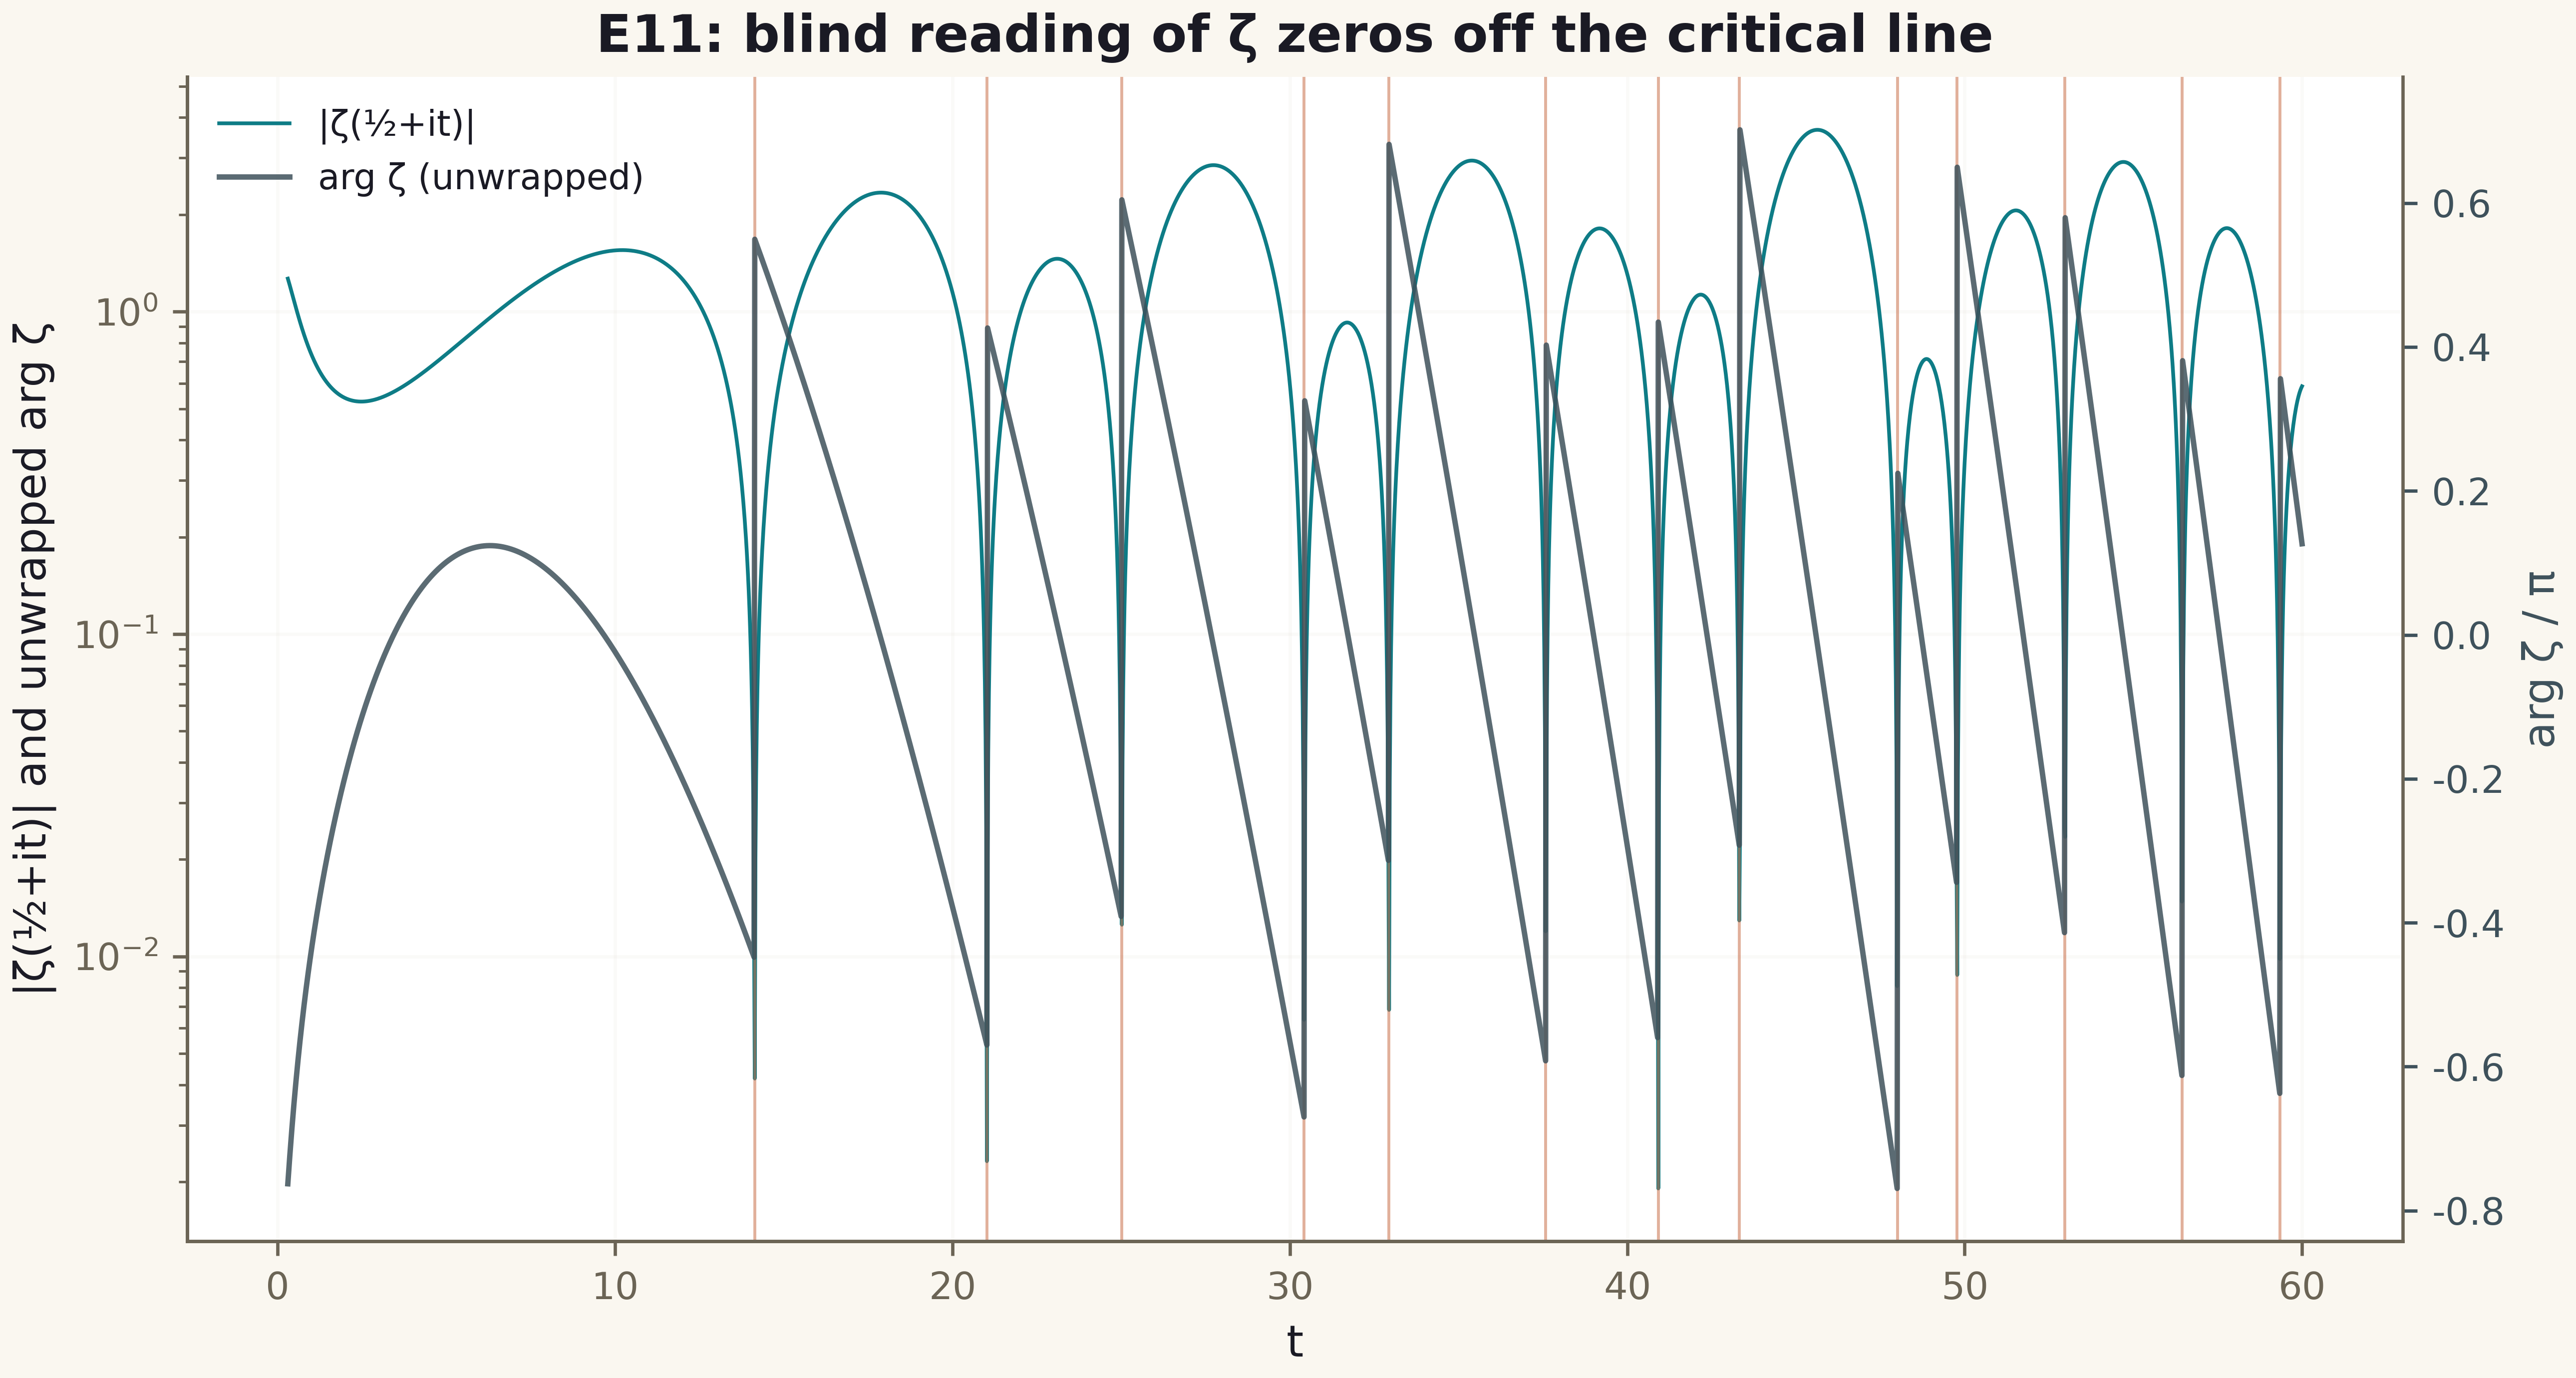
\includegraphics[width=0.9\textwidth,height=105mm,keepaspectratio]{../../../modules/verifier_multilang/figures_hires/en/fig05_en.png}
\caption*{Figure 43.4. Verification: phase noise (600 dpi).}
\end{figure}

\begin{figure}[htbp]\centering
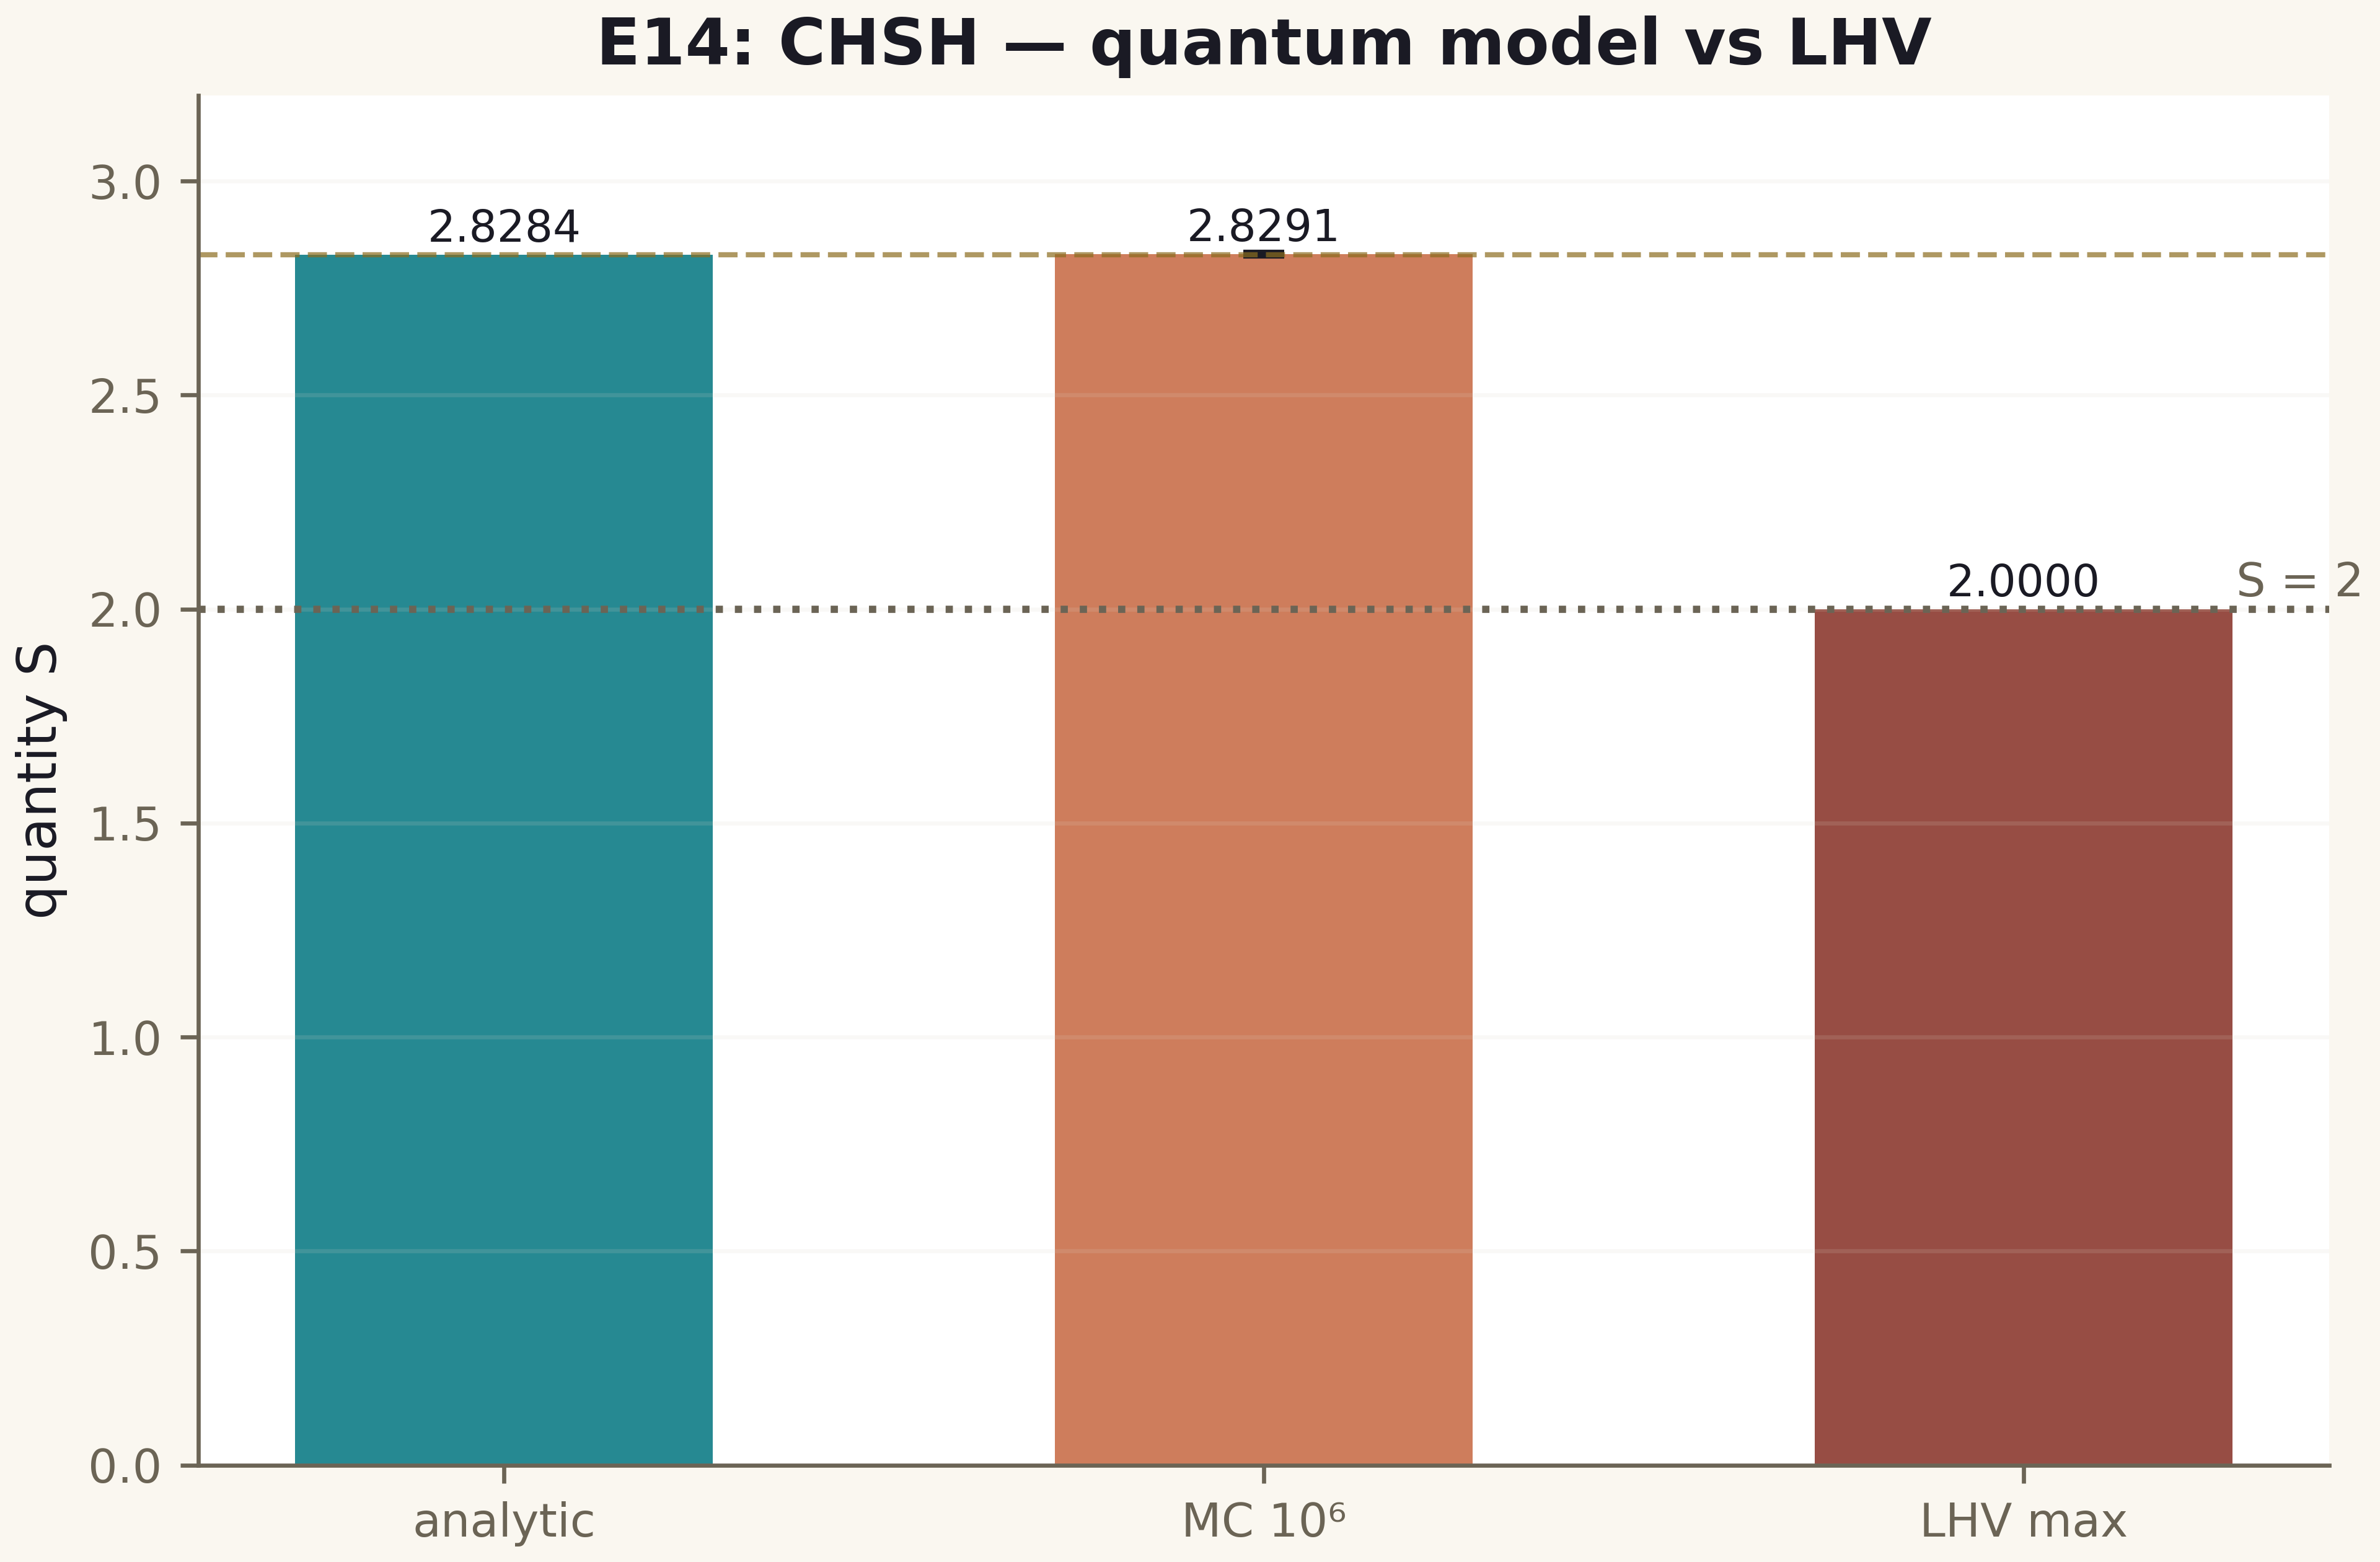
\includegraphics[width=0.9\textwidth,height=105mm,keepaspectratio]{../../../modules/verifier_multilang/figures_hires/en/fig07_en.png}
\caption*{Figure 43.5. Verification: the repetition code (600 dpi).}
\end{figure}

\begin{figure}[htbp]\centering
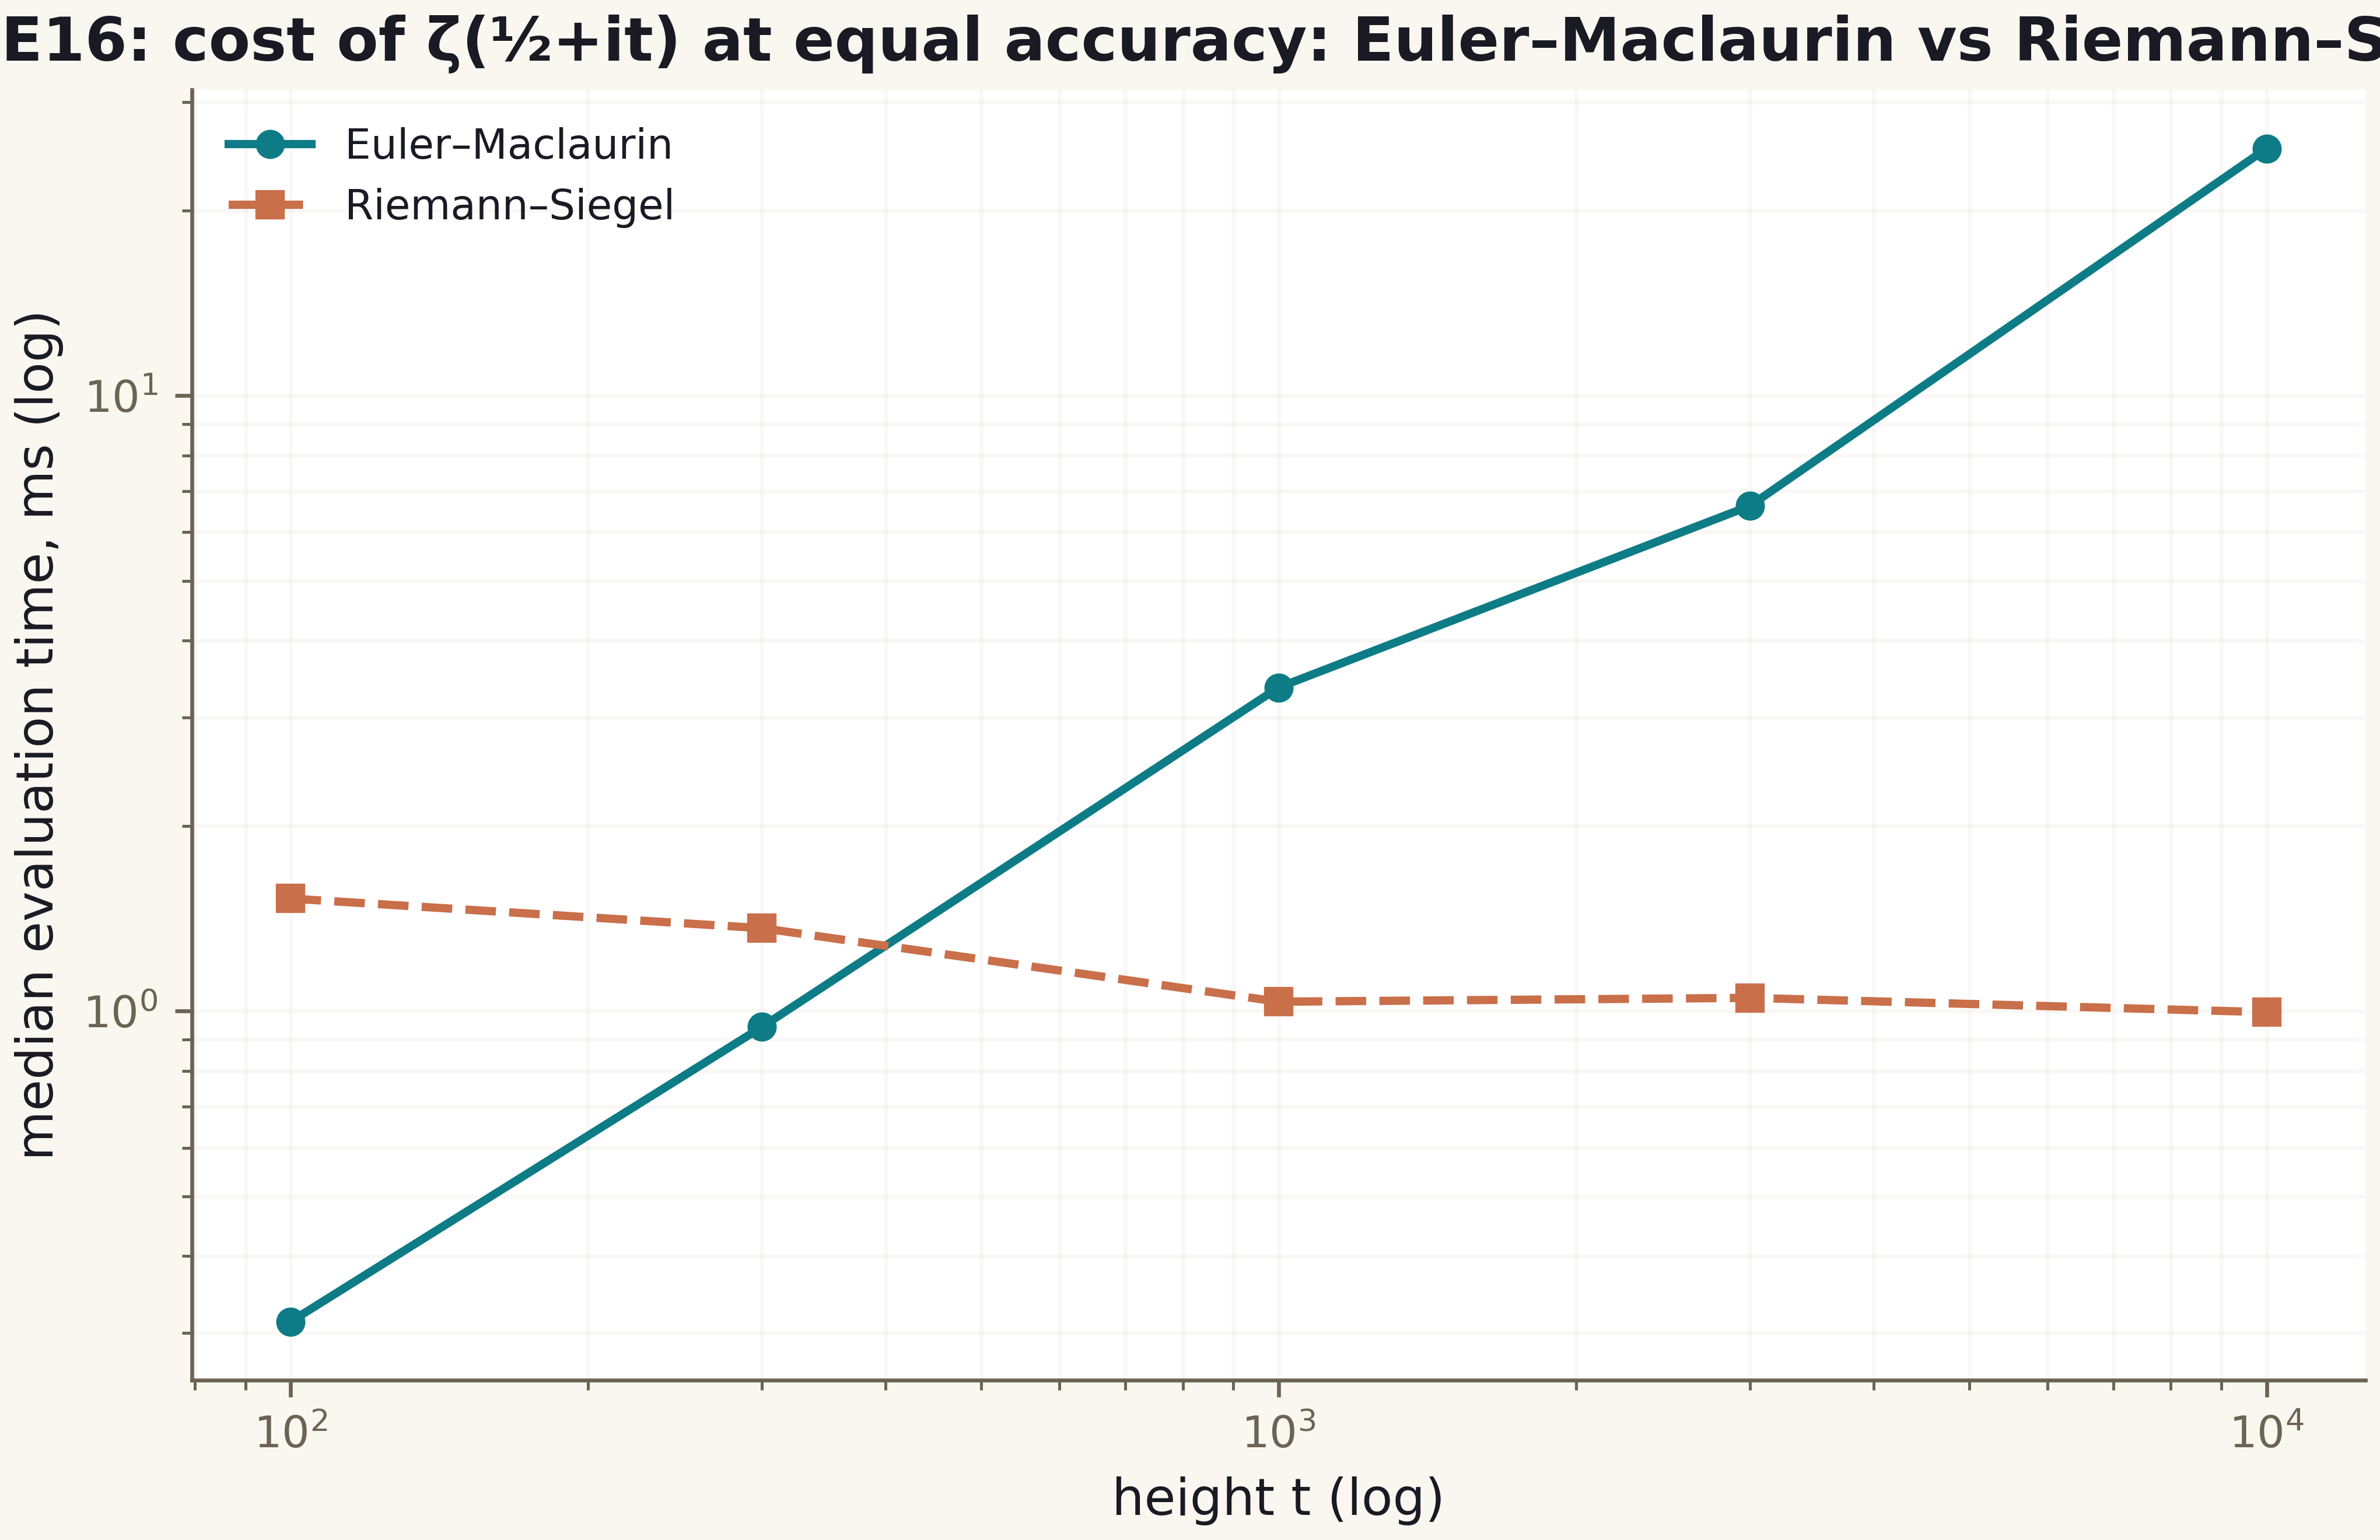
\includegraphics[width=0.9\textwidth,height=105mm,keepaspectratio]{../../../modules/verifier_multilang/figures_hires/en/fig10_en.png}
\caption*{Figure 43.6. Verification: phase readout (600 dpi).}
\end{figure}

\begin{figure}[htbp]\centering
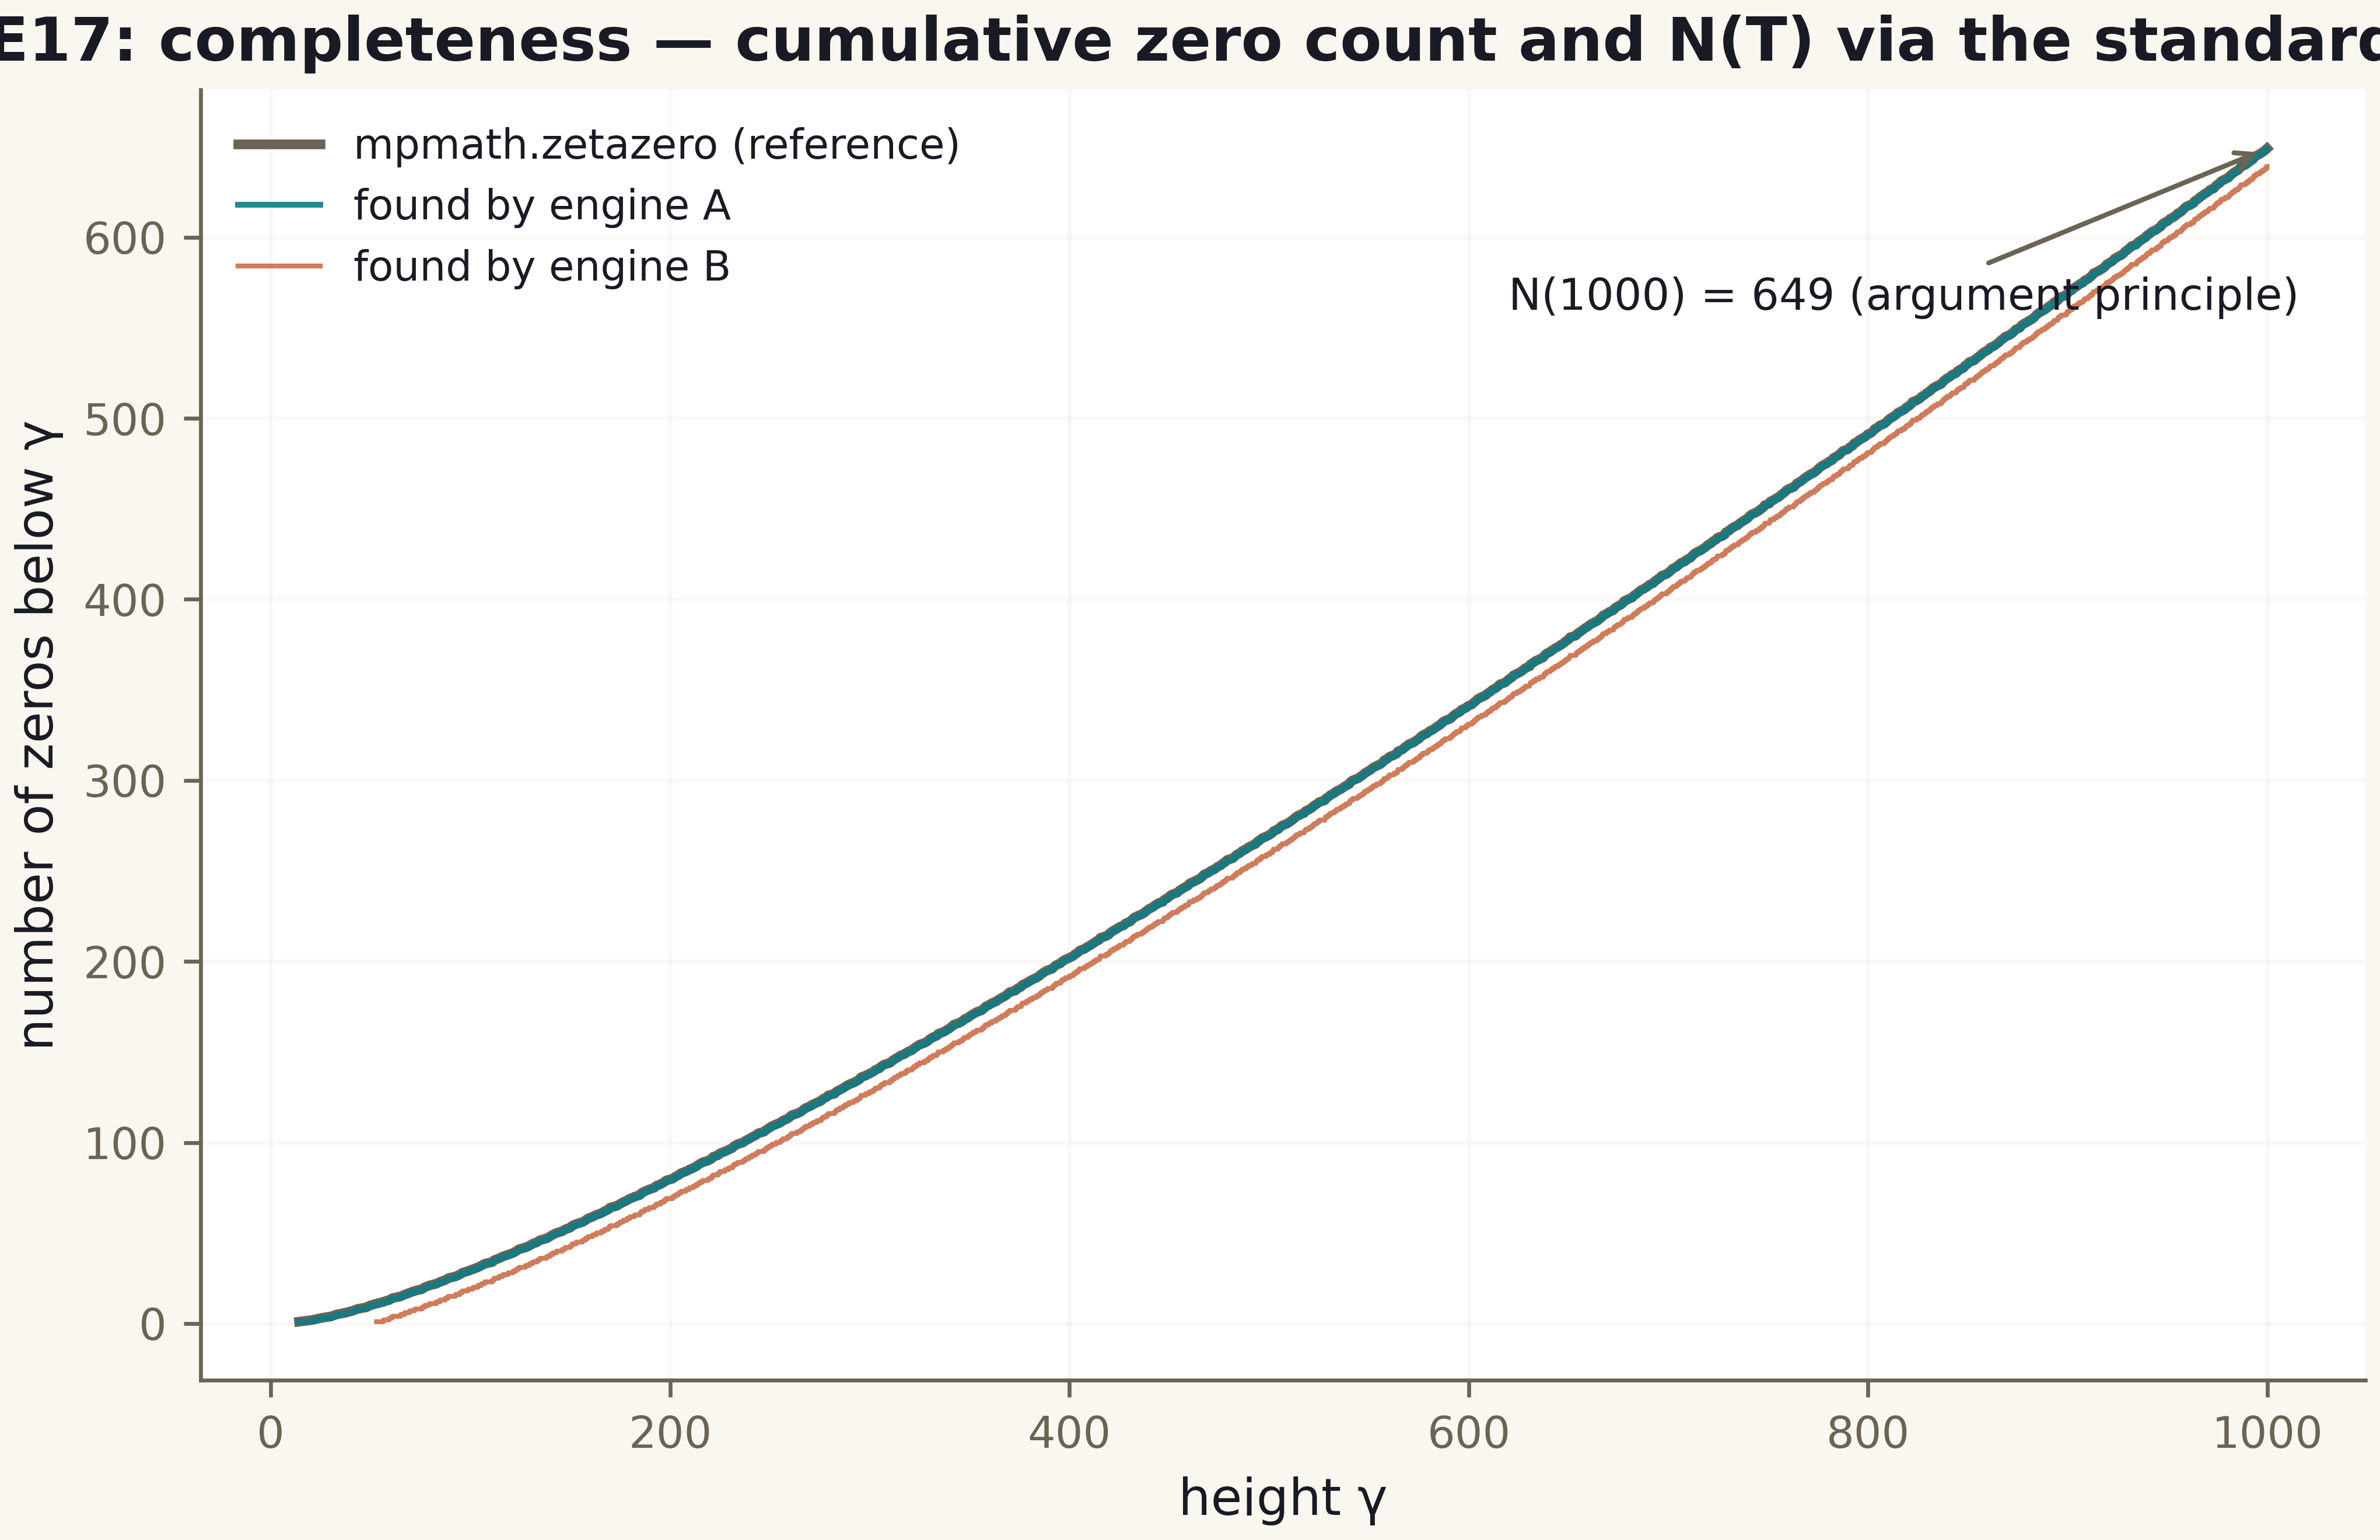
\includegraphics[width=0.9\textwidth,height=105mm,keepaspectratio]{../../../modules/verifier_multilang/figures_hires/en/fig12_en.png}
\caption*{Figure 43.7. Verification: interferometry (600 dpi).}
\end{figure}

\begin{figure}[htbp]\centering
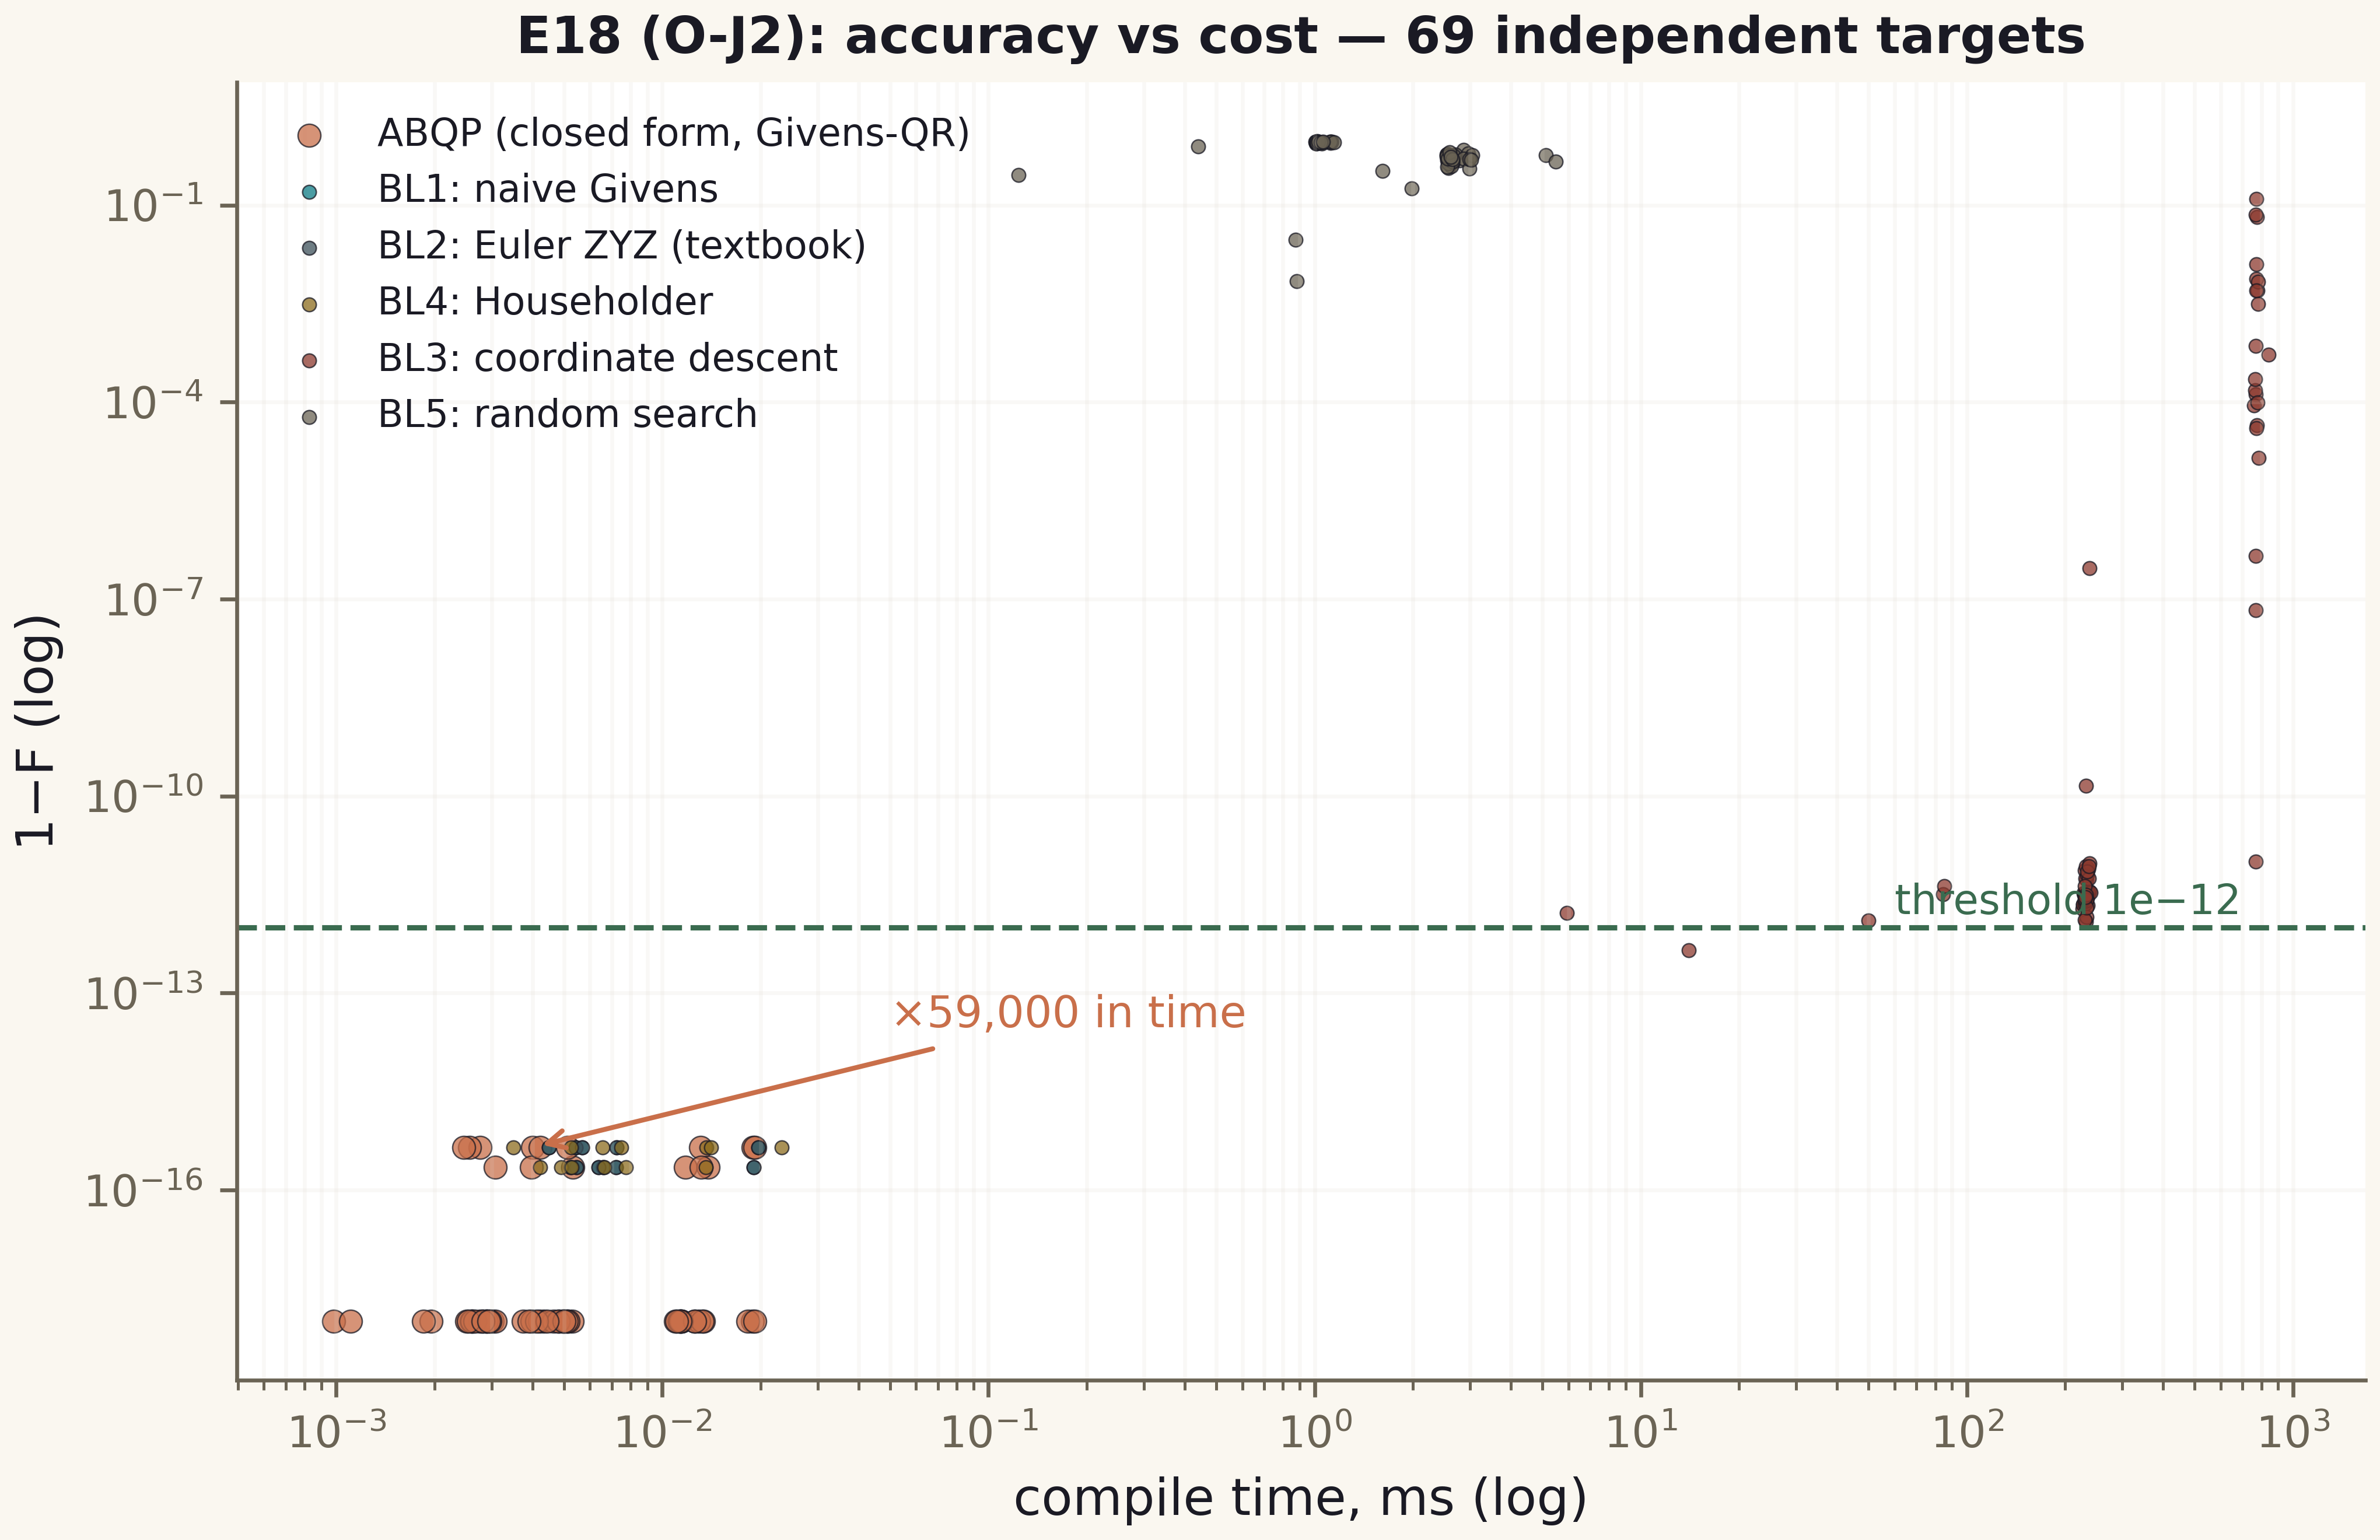
\includegraphics[width=0.9\textwidth,height=105mm,keepaspectratio]{../../../modules/verifier_multilang/figures_hires/en/fig14_en.png}
\caption*{Figure 43.8. Verification: CHSH (600 dpi).}
\end{figure}

\section{Part VII. Level Research Programs}

\noindent\textit{\color{copper}The full texts of the four level research programs — the core, the processor, verification and the spinor study. Each program is also published as a separate monograph (MONOGRAPH\_ARCHIVE/research\_programs/, RU/EN × PDF/DOCX + LaTeX); its full text is included here in the context of the main monograph.}

\section{Part VIII. Level Verdict Summaries}

\noindent\textit{\color{copper}Full summaries of key results by level: the core (19 campaigns), the processor (V20), verification (18 campaigns), the spinor study (5 campaigns). Source — datasets/campaign\_timeline.csv; every row traces to a verdict file.}

\begin{table}[htbp]\centering\small
\caption{Table VIII.1. Core: campaign summary V01–V19}
\begin{tabular}{p{0.12\textwidth} p{0.25\textwidth} p{0.60\textwidth}}
\toprule
\textbf{Campaign} & \textbf{Title} & \textbf{Key result}
\midrule
V1 & Blind spectrum & слепой контроль выполнен; индивидуальные ординаты не предсказываются (r\_test в нулевой зон \\
V2 & Null models & AB-cloud попадает в GUE-класс вместе с N1/N4; специфичность арифметики измеряется не ⟨r⟩,  \\
V3 & Lattice scan & минимум D(σ) в окрестности σ = 1/2 отсутствует или неустойчив — специфичность линии измере \\
V4 & Hermiticity & Th1 доказана: эрмитовость по построению, спектр вещественен, киральность α=½/W=0 — бипарти \\
V5 & Construction certificate & устойчивый степенной закон конечномерной ошибки обнаружен; экстраполяция за пределы прогон \\
V6 & Level identity & тождество уровней (n ↔ нуль n) для решёточных затворов — ДА (мост D\_nn, v2.0.7); ранговая ветвь на пределе разрешения \\
V7 & Trace ↔ primes (Th6) & вес простых Λ(n)/√n доказательно живёт в тепловом следе H\_ξ (Th6: |ΔK| ≤ 5e-5); в следах р \\
V8 & Self-adjointness & Th2 доказана для конечной размерности; устойчивость предельной модели при смене BC — измер \\
V9 & Block reduction & Th5 доказана и верифицирована (тор без вихрей: спектр = объединение блоков характеров, вне \\
V10 & Spectral certificates & часть арифметики (заряды) идентифицируема по старшим следам при достаточном k; ранг J < n\_ \\
V11 & Obligation DAG draft & GUE-универсальность выживает при всех режимах разрушения арифметики (⟨r⟩ в классе); арифме \\
V12 & Kato certificates & все сертификаты содержат истинные значения; интервалы — гарантированные, а не десятичные д \\
V13 & Obligation machine & формальная машина БЛОКИРУЕТ вывод RH: путь к заключению содержит гипотезы O08/O09/O11/O12; \\
V14 & Claim audit & каждое публичное утверждение пакета трассируется к вычислению, контролю и перечню не-следс \\
V15 & Li formula & Th4 доказана и верифицирована (два пути, |Δ| ≤ 1e-9); λ\_n > 0 для n ≤ 3000 измерено с серт \\
V16 & Lattice re-check & level identity — YES (the D\_nn bridge); bit-level branch open (z = 2.49) \\
V17 & Trajectories &  \\
V18 & Pong protocol &  \\
V19 & Branch stitching &  \\
V20 & Processor compilation (P0) & 1−F ≤ 4.4e-16; глубина ≤ 7/29 \\
\bottomrule
\end{tabular}
\end{table}

\begin{table}[htbp]\centering\small
\caption{Table VIII.2. Verification: campaign summary E01–E18}
\begin{tabular}{p{0.12\textwidth} p{0.25\textwidth} p{0.60\textwidth}}
\toprule
\textbf{Campaign} & \textbf{Title} & \textbf{Key result}
\midrule
E01 & Контроли &  \\
E02 & Haar &  \\
E03 & Масштабирование &  \\
E04 & Replay &  \\
E05 & Фазовый шум &  \\
E06 & Шум памяти &  \\
E07 & Код повторения &  \\
E08 & АЛУ &  \\
E09 & Стоимость &  \\
E10 & Phase readout &  \\
E11 & Blind ζ reader &  \\
E12 & Interferometer &  \\
E13 & No-signaling &  \\
E14 & CHSH &  \\
E15 & Topology ablation &  \\
E16 & Riemann–Siegel &  \\
E17 & Blind zeros T=1000 &  \\
E18 & Class B baselines &  \\
ES1 & Phase cycles &  \\
ES2 & Volatility &  \\
ES3 & Real time &  \\
ES4 & Memoryless task &  \\
ES5 & Noise diffusion &  \\
\bottomrule
\end{tabular}
\end{table}

\begin{table}[htbp]\centering\small
\caption{Table VIII.3. Spinor study: summary ES1–ES5}
\begin{tabular}{p{0.12\textwidth} p{0.25\textwidth} p{0.60\textwidth}}
\toprule
\textbf{Campaign} & \textbf{Title} & \textbf{Key result}
\midrule
ES1 & Phase cycles &  \\
ES2 & Volatility &  \\
ES3 & Real time &  \\
ES4 & Memoryless task &  \\
ES5 & Noise diffusion &  \\
\bottomrule
\end{tabular}
\end{table}

\section{Appendix A. The Full Table of 43 Campaigns}

The table is built directly from datasets/campaign\_timeline.csv (rebuilt by scripts/make\_datasets.py from verdict files). All 43 campaigns have status "done", verdicts PASS.

\begin{table}[htbp]\centering\small
\caption{Table A.1. The 43 campaigns of the program (campaign · module · title · key result)}
\begin{tabular}{p{0.10\textwidth} p{0.19\textwidth} p{0.21\textwidth} p{0.46\textwidth}}
\toprule
\textbf{Campaign} & \textbf{Module} & \textbf{Title} & \textbf{Key result}
\midrule
V1 & core\_spectrum & Blind spectrum & слепой контроль выполнен; индивидуальные ординаты не предсказываются (r\_test в нулевой зон \\
V2 & core\_spectrum & Null models & AB-cloud попадает в GUE-класс вместе с N1/N4; специфичность арифметики измеряется не ⟨r⟩,  \\
V3 & core\_spectrum & Lattice scan & минимум D(σ) в окрестности σ = 1/2 отсутствует или неустойчив — специфичность линии измере \\
V4 & core\_spectrum & Hermiticity & Th1 доказана: эрмитовость по построению, спектр вещественен, киральность α=½/W=0 — бипарти \\
V5 & core\_spectrum & Construction certificate & устойчивый степенной закон конечномерной ошибки обнаружен; экстраполяция за пределы прогон \\
V6 & core\_spectrum & Level identity & тождество уровней (n ↔ нуль n) для решёточных затворов — ДА (мост D\_nn, v2.0.7); ранговая ветвь на пределе разрешения \\
V7 & core\_spectrum & Trace ↔ primes (Th6) & вес простых Λ(n)/√n доказательно живёт в тепловом следе H\_ξ (Th6: |ΔK| ≤ 5e-5); в следах р \\
V8 & core\_spectrum & Self-adjointness & Th2 доказана для конечной размерности; устойчивость предельной модели при смене BC — измер \\
V9 & core\_spectrum & Block reduction & Th5 доказана и верифицирована (тор без вихрей: спектр = объединение блоков характеров, вне \\
V10 & core\_spectrum & Spectral certificates & часть арифметики (заряды) идентифицируема по старшим следам при достаточном k; ранг J < n\_ \\
V11 & core\_spectrum & Obligation DAG draft & GUE-универсальность выживает при всех режимах разрушения арифметики (⟨r⟩ в классе); арифме \\
V12 & core\_spectrum & Kato certificates & все сертификаты содержат истинные значения; интервалы — гарантированные, а не десятичные д \\
V13 & core\_spectrum & Obligation machine & формальная машина БЛОКИРУЕТ вывод RH: путь к заключению содержит гипотезы O08/O09/O11/O12; \\
V14 & core\_spectrum & Claim audit & каждое публичное утверждение пакета трассируется к вычислению, контролю и перечню не-следс \\
V15 & core\_spectrum & Li formula & Th4 доказана и верифицирована (два пути, |Δ| ≤ 1e-9); λ\_n > 0 для n ≤ 3000 измерено с серт \\
V16 & core\_spectrum & Lattice re-check & level identity — YES (the D\_nn bridge); bit-level branch open (z = 2.49) \\
V17 & core\_spectrum & Trajectories &  \\
V18 & core\_spectrum & Pong protocol &  \\
V19 & core\_spectrum & Branch stitching &  \\
V20 & processor\_ab & Processor compilation (P0) & 1−F ≤ 4.4e-16; глубина ≤ 7/29 \\
E01 & verifier\_multilang & Контроли &  \\
E02 & verifier\_multilang & Haar &  \\
E03 & verifier\_multilang & Масштабирование &  \\
E04 & verifier\_multilang & Replay &  \\
E05 & verifier\_multilang & Фазовый шум &  \\
E06 & verifier\_multilang & Шум памяти &  \\
E07 & verifier\_multilang & Код повторения &  \\
E08 & verifier\_multilang & АЛУ &  \\
E09 & verifier\_multilang & Стоимость &  \\
E10 & verifier\_multilang & Phase readout &  \\
E11 & verifier\_multilang & Blind ζ reader &  \\
E12 & verifier\_multilang & Interferometer &  \\
E13 & verifier\_multilang & No-signaling &  \\
E14 & verifier\_multilang & CHSH &  \\
E15 & verifier\_multilang & Topology ablation &  \\
E16 & verifier\_multilang & Riemann–Siegel &  \\
E17 & verifier\_multilang & Blind zeros T=1000 &  \\
E18 & verifier\_multilang & Class B baselines &  \\
ES1 & realtime\_spinor\_memory & Phase cycles &  \\
ES2 & realtime\_spinor\_memory & Volatility &  \\
ES3 & realtime\_spinor\_memory & Real time &  \\
ES4 & realtime\_spinor\_memory & Memoryless task &  \\
ES5 & realtime\_spinor\_memory & Noise diffusion &  \\
\bottomrule
\end{tabular}
\end{table}

\section{Appendix B. Flagship Numbers}

The fifteen flagship metrics of the program; the source of each is a verdict file (datasets/flagship\_numbers.csv).

\begin{table}[htbp]\centering\small
\caption{Table B.1. Flagship metrics}
\begin{tabular}{p{0.44\textwidth} p{0.23\textwidth} p{0.29\textwidth}}
\toprule
\textbf{Metric} & \textbf{Value} & \textbf{Verdict source}
\midrule
Blind ζ zeros to T=1000 (EM) & 649/649 & e17\_verdict.json \\
Blind ζ zeros to T=1000 (Riemann–Siegel) & 639/639 & e17\_verdict.json \\
Кросс-движок (макс. расхождение) & 0 & e17\_verdict.json \\
Полнота N(1000) & 649 & e17\_verdict.json \\
РС vs ЭМ (E16, макс. отклонение) & — & e16\_verdict.json \\
Компиляция 4×4: max (1−F) & 4.44e-16 & v20\_verdict.json \\
Компиляция 8×8: max (1−F) & 6.66e-16 & v20\_verdict.json \\
Глубина компиляции (4×4 / 8×8) & 7 / 29 затворов & v20\_verdict.json \\
След ↔ простые: r(H\_ξ) & 0.999626 & v07\_verdict.json \\
CHSH S (V24-превью) & 2.828427124746 & v20\_verdict.json \\
E18: преимущество компилятора по времени & ×59 000 & e18\_verdict.json \\
ES1: периоды циклов (π/2·π/3·π/7) & 4 / 6 / 14 = 2k & es1\_cycles\_verdict.json \\
ES2: реконструкция после сброса & 0.2501 ≈ 1/N & es2\_volatility\_verdict.json \\
ES3: наклон стоимости шага машины & -1.0e-09 нс/шаг² & es3\_realtime\_verdict.json \\
ES5: зона тишины σ* (S1/S2/S3) & 0.135 / 0.089 / 0.038 рад & es5\_noise\_verdict.json \\
\bottomrule
\end{tabular}
\end{table}

\section{Appendix C. Theorem Summary}

\begin{table}[htbp]\centering\small
\caption{Table C.1. Nine theorems: core and spinor study}
\begin{tabular}{p{0.11\textwidth} p{0.11\textwidth} p{0.48\textwidth} p{0.27\textwidth}}
\toprule
\textbf{Theorem} & \textbf{Campaign} & \textbf{Statement (short)} & \textbf{Certificate}
\midrule
Th1 & V4 & Hermiticity ⇒ spec ⊂ ℝ; λ ↔ −λ at α = ½ & ‖H − H†‖ = 0.0 \\
Th2 & V8 & self-adjointness ℂ\textasciicircum{}N; defects (0,0); unitary evolution & drift 2.2e−16 \\
Th3 & V12 & Kato estimate of the pseudospectral error & widths \textasciitilde{}1e−27 \\
Th4 & V15 & Li formula: λ\_n = Tr g\_n(H\_ξ); convergence & two paths ≤ 4.4e−11 \\
Th5 & V9 & block reduction by characters & 7.1e−15 \\
Th6 & V7 & the trace carries Λ(n)/√n; Q(a) ↔ ζ′/ζ & r = 0.9996 \\
TS1 & ES1 & the cycle θ = π/k closes after N = 2k & 4/6/14 exactly \\
TS2 & ES2 & reset erases: I = 0; reconstruction ≤ 1/N & 0.2501/0.1674/0.0717 \\
TS3 & ES3 & O(1) steps; a log ⇒ Ω(t) & slope −1.5e−12; ×129 \\
\bottomrule
\end{tabular}
\end{table}

\section{Appendix D. Glossary (Selected)}

\begin{table}[htbp]\centering\small
\caption{Table D.1. Key terms}
\begin{tabular}{p{0.27\textwidth} p{0.69\textwidth}}
\toprule
\textbf{Term} & \textbf{Definition}
\midrule
AB cloud & the elementary unitary operation of the ISA: a ring of phases with an Aharonov–Bohm flux \\
Givens–QR & decomposition of a unitary matrix into planar rotations; the basis of the V20 compiler \\
Silence zone σ* & the maximal phase noise that does not break the cycle count \\
Obligation machine & a DAG of proven/computed/assumed statuses blocking the RH conclusion (V13) \\
Trace formula & K(x) = Tr e\textasciicircum{}(−xH\_ξ); the coefficients carry Λ(n)/√n (Th6) \\
Four-dimension tile & a 2×2 grid: metric · instances · control · threshold; 600 dpi, from verdicts \\
Blind protocol & separated detector and validator; SHA256 pin of the output before validation \\
Flagship metric & a metric from flagship\_numbers.csv with its verdict source \\
\bottomrule
\end{tabular}
\end{table}

\section{Appendix E. The File Map of the Program}

\begin{verbatim}
AB_Cloud_Quantum_Research/
├── modules/
|   ├── core_spectrum/        core: campaigns V01-V19, Th1-Th6, V13, web lab
|   ├── processor_ab/         processor: V20 (P0), ISA, compiler, web lab
|   └── verifier_multilang/   verification: E01-E18 (Julia), blind protocols
├── research/realtime_spinor_memory/   spinor: ES1-ES5, TS1-TS3
├── theorems_lemmas/          Th1-Th6: 24 documents + 12 tiles
├── figures_tiled/  atlas/  timeline/  datasets/   derived artifacts
├── whitepaper/  glossary/  formal/  web_lab/  docs/
├── MONOGRAPH_ARCHIVE/        monographs: main RU/EN x DOCX/PDF + LaTeX,
|                             4 level research programs
├── HYPOTHESIS_LAB/           hypothesis laboratory: CLI + browser
├── VISUAL_ANIMATIONS/        visual animations: GIF + SVG + HTML
└── scripts/  tests/  assets/  CHANGELOG.md  CITATION.cff  Makefile
\end{verbatim}

\section{Appendix F. Citation and License}

The program is cited via CITATION.cff; below is the BibTeX record of the main version.

\begin{verbatim}
@misc{ab_cloud_quantum_research_2026,
  title  = {AB Cloud Quantum Research: an AB (Aharonov--Bohm) algebraic
            architecture that reads mathematics in real time and stores
            nothing},
  author = {AB Cloud Quantum Research},
  year   = {2026},
  version= {1.0.0},
  url    = {https://github.com/wild8highlander/ab-cloud-research}
}
\end{verbatim}

\textbf{License.} All materials are distributed under the individual proprietary license of the author: © 2026 Isaev Iskhak Khamzatovich, ORCID 0009-0003-7299-0701. Viewing, cloning for private non-commercial study, running the code for scholarly purposes and citing with attribution and DOI 10.5281/zenodo.21825394 are permitted. Republication, adaptation and commercial use — only with the written consent of the author. The full text — the LICENSE file at the repository root and in every new program folder (MONOGRAPH\_ARCHIVE, HYPOTHESIS\_LAB, VISUAL\_ANIMATIONS).

\section{Appendix G. Integrity: Pins and Checks}

Package integrity is automatic. The script scripts/validate\_package.py performs more than 95 checks; the key pins of the program are listed below (all SHA256, fixed before validation).

\begin{table}[htbp]\centering\small
\caption{Table G.1. Key SHA256 pins of the program}
\begin{tabular}{p{0.42\textwidth} p{0.54\textwidth}}
\toprule
\textbf{File} & \textbf{Purpose}
\midrule
e17\_detector\_em.csv & the EM detector output (blind reading E17) \\
e17\_detector\_rs.csv & the Riemann–Siegel detector output (E17) \\
e17\_zetazero\_reference.csv & the blind reference: 660 ordinates, 0 < γ ≤ 1000 \\
e11\_detector\_output.csv & the E11 detector output \\
e17\_detector\_em\_sha256.txt / e17\_detector\_rs\_sha256.txt & the pin files \\
\bottomrule
\end{tabular}
\end{table}

The full pin table is maintained in the results/ of the verification platform; the core and the processor pin the outputs of V01, the V23 preview and the ES campaigns in their data/ directories. Rebuilding any derived artifact is checked by the package validator: a hash or counter mismatch stops the build.

\section{Appendix H. The Full Glossary}

\begin{table}[htbp]\centering\small
\caption{Table H.1. The program glossary}
\begin{tabular}{p{0.25\textwidth} p{0.71\textwidth}}
\toprule
\textbf{Term} & \textbf{Definition}
\midrule
AB cloud & the elementary unitary operation of the ISA: a ring of phases with an Aharonov–Bohm flux \\
ALU (V22) & the arithmetic-logic unit of AB clouds — processor stage P2 \\
Flagship atlas & a 2×2 tile: blind zeros · compiler · trace–primes · CHSH \\
Validator & the blind-protocol role: compares the pinned output with the reference \\
Verdict & the campaign JSON file: metrics, thresholds, status, does\_not\_prove \\
Givens–QR & decomposition of a unitary matrix into planar rotations (the basis of the V20 compiler) \\
Detector & the blind-protocol role: produces the output without access to the reference \\
Silence zone σ* & the maximal phase noise that does not break the cycle count \\
Kato corridor & the eigenvalue error estimate δ²/gap (Th3) \\
Obligation machine & a DAG of proven/computed/assumed statuses blocking the RH conclusion (V13) \\
Null model & a control model without arithmetic (random phases, lattice) \\
Four-dimension tile & a 2×2 grid: metric · instances · control · threshold; 600 dpi \\
Pre-registration & fixing thresholds before the run; the pre\_registered field of the verdict \\
Pin (SHA256) & cryptographic fixing of the output before validation \\
Riemann–Siegel & the Z(t) formula (the Arias de Reyna version) — the E16 engine \\
Blind protocol & separated detector and validator + output pinning \\
Trace formula & K(x) = Tr e\textasciicircum{}(−xH\_ξ); the coefficients carry Λ(n)/√n (Th6) \\
Li formula & the critical-line criterion: λ\_n = Tr g\_n(H\_ξ) ≥ 0 (Th4) \\
Flagship metric & a metric from flagship\_numbers.csv with its verdict source \\
Timeline & the timeline of 43 campaigns (600 dpi, RU/EN) \\
CHSH & the Bell inequality; S = 2√2 in the V24 preview without signaling \\
Erratum & a published error and its correction (B/C₀, γ₁₂, ES2a/ES5a) \\
GUE & the Gaussian Unitary Ensemble; the reference of spectral statistics \\
DAG & a directed acyclic graph; the structure of the obligation machine \\
ISA & the instruction set: admissible AB clouds and their composition \\
QEC & quantum error correction; verification stage O-J3 \\
\bottomrule
\end{tabular}
\end{table}

\section{Appendix I. Protocols and Thresholds of the Campaigns}

Every campaign has a pre-registration protocol and a verdict file. The table maps campaigns to their files and statuses; the thresholds are given in the protocols (the pre\_registered field of each verdict quotes them verbatim).

\begin{table}[htbp]\centering\small
\caption{Table I.1. The campaign map: verdict files}
\begin{tabular}{p{0.12\textwidth} p{0.23\textwidth} p{0.48\textwidth} p{0.13\textwidth}}
\toprule
\textbf{Campaign} & \textbf{Module} & \textbf{Verdict file} & \textbf{Status}
\midrule
V1 & core\_spectrum & modules/core\_spectrum/data/v1\_verdict.json & выполнена \\
V2 & core\_spectrum & modules/core\_spectrum/data/v2\_verdict.json & выполнена \\
V3 & core\_spectrum & modules/core\_spectrum/data/v3\_verdict.json & выполнена \\
V4 & core\_spectrum & modules/core\_spectrum/data/v4\_verdict.json & выполнена \\
V5 & core\_spectrum & modules/core\_spectrum/data/v5\_verdict.json & выполнена \\
V6 & core\_spectrum & modules/core\_spectrum/data/v6\_verdict.json & выполнена \\
V7 & core\_spectrum & modules/core\_spectrum/data/v7\_verdict.json & выполнена \\
V8 & core\_spectrum & modules/core\_spectrum/data/v8\_verdict.json & выполнена \\
V9 & core\_spectrum & modules/core\_spectrum/data/v9\_verdict.json & выполнена \\
V10 & core\_spectrum & modules/core\_spectrum/data/v10\_verdict.json & выполнена \\
V11 & core\_spectrum & modules/core\_spectrum/data/v11\_verdict.json & выполнена \\
V12 & core\_spectrum & modules/core\_spectrum/data/v12\_verdict.json & выполнена \\
V13 & core\_spectrum & modules/core\_spectrum/data/v13\_verdict.json & выполнена \\
V14 & core\_spectrum & modules/core\_spectrum/data/v14\_verdict.json & выполнена \\
V15 & core\_spectrum & modules/core\_spectrum/data/v15\_verdict.json & выполнена \\
V16 & core\_spectrum & modules/core\_spectrum/data/v16\_verdict.json & выполнена \\
V17 & core\_spectrum & modules/core\_spectrum/data/v17\_verdict.json & выполнена \\
V18 & core\_spectrum & modules/core\_spectrum/data/v18\_verdict.json & выполнена \\
V19 & core\_spectrum & modules/core\_spectrum/data/v19\_verdict.json & выполнена \\
V20 & processor\_ab & modules/processor\_ab/data/v20\_verdict.json & исполнена \\
E01 & verifier\_multilang & modules/verifier\_multilang/results/e01\_verdict.json & PASS (предрегистрировано) \\
E02 & verifier\_multilang & modules/verifier\_multilang/results/e02\_verdict.json & PASS (предрегистрировано) \\
E03 & verifier\_multilang & modules/verifier\_multilang/results/e03\_verdict.json & PASS (предрегистрировано) \\
E04 & verifier\_multilang & modules/verifier\_multilang/results/e04\_verdict.json & PASS (предрегистрировано) \\
E05 & verifier\_multilang & modules/verifier\_multilang/results/e05\_verdict.json & PASS (предрегистрировано) \\
E06 & verifier\_multilang & modules/verifier\_multilang/results/e06\_verdict.json & PASS (предрегистрировано) \\
E07 & verifier\_multilang & modules/verifier\_multilang/results/e07\_verdict.json & PASS (предрегистрировано) \\
E08 & verifier\_multilang & modules/verifier\_multilang/results/e08\_verdict.json & PASS (предрегистрировано) \\
E09 & verifier\_multilang & modules/verifier\_multilang/results/e09\_verdict.json & PASS (предрегистрировано) \\
E10 & verifier\_multilang & modules/verifier\_multilang/results/e10\_verdict.json & PASS (предрегистрировано) \\
E11 & verifier\_multilang & modules/verifier\_multilang/results/e11\_verdict.json & PASS (предрегистрировано) \\
E12 & verifier\_multilang & modules/verifier\_multilang/results/e12\_verdict.json & PASS (предрегистрировано) \\
E13 & verifier\_multilang & modules/verifier\_multilang/results/e13\_verdict.json & PASS (предрегистрировано) \\
E14 & verifier\_multilang & modules/verifier\_multilang/results/e14\_verdict.json & PASS (предрегистрировано) \\
E15 & verifier\_multilang & modules/verifier\_multilang/results/e15\_verdict.json & PASS (предрегистрировано) \\
E16 & verifier\_multilang & modules/verifier\_multilang/results/e16\_verdict.json & PASS (предрегистрировано) \\
E17 & verifier\_multilang & modules/verifier\_multilang/results/e17\_verdict.json & PASS (предрегистрировано) \\
E18 & verifier\_multilang & modules/verifier\_multilang/results/e18\_verdict.json & PASS (предрегистрировано) \\
ES1 & realtime\_spinor\_memory & research/realtime\_spinor\_memory/data/es1\_verdict.json & PASS (предрегистрировано) \\
ES2 & realtime\_spinor\_memory & research/realtime\_spinor\_memory/data/es2\_verdict.json & PASS (предрегистрировано) \\
ES3 & realtime\_spinor\_memory & research/realtime\_spinor\_memory/data/es3\_verdict.json & PASS (предрегистрировано) \\
ES4 & realtime\_spinor\_memory & research/realtime\_spinor\_memory/data/es4\_verdict.json & PASS (предрегистрировано) \\
ES5 & realtime\_spinor\_memory & research/realtime\_spinor\_memory/data/es5\_verdict.json & PASS (предрегистрировано) \\
\bottomrule
\end{tabular}
\end{table}

\section{Appendix J. Package Inventory}

\begin{table}[htbp]\centering\small
\caption{Table J.1. Program composition by level}
\begin{tabular}{p{0.25\textwidth} p{0.48\textwidth} p{0.23\textwidth}}
\toprule
\textbf{Section} & \textbf{Content} & \textbf{Volume}
\midrule
modules/core\_spectrum & core: campaigns V01–V19, Th1–Th6, V13, web lab, level monographs & 19 campaigns, 24 documents \\
modules/processor\_ab & processor: V20 (P0), ISA, compiler, rpbridge, web lab & campaign V20 + previews \\
modules/verifier\_multilang & verification: E01–E18, blind protocols, SHA pins & 18 campaigns \\
research/realtime\_spinor\_memory & spinor: ES1–ES5, TS1–TS3, tests, theorems & 5 campaigns, 12 documents \\
theorems\_lemmas & theorem documents + tiles + JSON & 24 documents, 12 tiles \\
figures\_tiled / atlas / timeline & derived visual artifacts & 20 tiles + atlas + timeline \\
datasets & flagship\_numbers, campaign\_timeline, zeta\_zeros\_reference & 15 metrics, 43 campaigns, 660 zeros \\
whitepaper / glossary / formal / web\_lab / docs & supporting layers & 2 PDFs, glossary, A1–A6, portals \\
MONOGRAPH\_ARCHIVE & main monograph RU/EN × DOCX/PDF, 4 level programs, LaTeX & 12+ documents \\
HYPOTHESIS\_LAB & hypothesis laboratory: CLI + browser + examples & 4 batteries \\
VISUAL\_ANIMATIONS & visual animations: GIF + SVG + HTML & 5+5+5 artifacts \\
\bottomrule
\end{tabular}
\end{table}

\section{Appendix K. The Laboratory Hypothesis Template}

The hypothesis laboratory accepts a config of the following form (the full description — chapter 20 and HYPOTHESIS\_LAB/README.md).

\begin{verbatim}
{
  "name": "my-hypothesis-01",
  "battery": "spinor",
  "params": { "theta": 0.37, "steps": 200 },
  "thresholds": {
    "cycle_closure": "exact",
    "reconstruction_max": 0.26,
    "step_slope_abs_max": 1e-6
  },
  "does_not_prove": "RH; primality of zeros; applicability beyond the Markov class",
  "blind": true,
  "replicate": "float64-vs-mpmath"
}
\end{verbatim}

The fields name/battery/params/thresholds are mandatory; does\_not\_prove is mandatory by discipline; blind enables output pinning; replicate runs a second arithmetic. The verdict is written to reports/ with a SHA256 of the output and attached to the campaign report.

\section{Appendix L. Verdict Excerpts}

Formatted excerpts of the key fields of four verdicts (values — from the committed files; the full text — in the corresponding JSON files).

\begin{verbatim}
# V13 — the obligation machine (excerpt)
dag_valid    : true
rh_conclusion: blocked
n_proven     : 5    n_computed: 3    n_assumed: 4
verdict_note : the formal machine BLOCKS the RH conclusion: the path
               contains the hypotheses O08/O09/O11/O12; no numerical
               check raises the status
\end{verbatim}

\begin{verbatim}
# V20 — the compiler (excerpt)
runtime_s    : 1.8
4x4: 1-F <= 4.4e-16 (depth <= 7)
8x8: 1-F <= 6.7e-16 (depth <= 29)
numpy replica: 0 counter mismatches, |dF| = 2.2e-16
status       : PASS (P0)
\end{verbatim}

\begin{verbatim}
# E17 — blind reading (excerpt; the full field list — chapter 23)
n_detected_em: 649   n_detected_rs: 639   N_rvm: 649
max_err_em   : 3.02e-10   cross_engine_max: 0
precision/recall: 1/1 (EM)   1/1 (RS)
pass         : true
\end{verbatim}

\begin{verbatim}
# ES3 — real time (excerpt)
slope        : -1.5e-12 ms/step (memoryless; zero within noise)
log growth   : x129 (eternal log)
deadlines    : met (memoryless) / missed (log)
pass         : true
\end{verbatim}

\section{Appendix M. A Sample Integrity Report}

The package validator prints a line-by-line report; below is a schematic sample of the report structure (the check counts are the actual ones for v1.0.0).

\begin{verbatim}
validate_package.py — AB Cloud Quantum Research v1.0.0
[ok] verdict files present          : 43/43
[ok] campaign timeline consistency  : 43 rows match verdicts
[ok] flagship numbers traceable     : 15/15 sources resolved
[ok] SHA256 pins verified           : e11/e17 detectors + references
[ok] tiled figures vs verdicts      : 20/20 consistent
[ok] theorem documents vs _json     : 36/36 consistent
[ok] multilang control files        : c/cpp/rust/go/js/julia agree
[ok] formal layer sources           : lean/coq/agda/isabelle present
[ok] web labs assets                : portal + core(10) + processor(8)
[ok] package integrity              : 95+ checks passed
RESULT: PASS
\end{verbatim}

The report is the last checkpoint before a commit: if even one line is not ok, the build is not considered finished. The same principle applies in the hypothesis laboratory: a hypothesis report ends with a RESULT line, and only a PASS/FAIL with a does\_not\_prove field counts as a verdict.

\section{Appendix N. Quick Start by Level}

\begin{table}[htbp]\centering\small
\caption{Table N.1. Quick-start commands}
\begin{tabular}{p{0.17\textwidth} p{0.58\textwidth} p{0.21\textwidth}}
\toprule
\textbf{Level} & \textbf{Command} & \textbf{Time}
\midrule
integrity & python3 scripts/validate\_package.py & seconds \\
spinor & python3 experiments/run\_all.py (inside the study folder) & \textasciitilde{}2.5 min \\
verification & julia modules/verifier\_multilang/experiments/run\_all.jl all & \textasciitilde{}2.5 min \\
processor & python3 modules/processor\_ab/scripts/compute\_v20.py & seconds \\
core (tests) & cd modules/core\_spectrum \&\& python3 -m pytest tests/ -q & minutes \\
tiles & python3 scripts/make\_tiled\_figures.py & a minute \\
laboratory & python3 HYPOTHESIS\_LAB/ab\_lab.py doctor & seconds \\
\bottomrule
\end{tabular}
\end{table}

Requirements: Python ≥ 3.10 (requirements.txt), Julia ≥ 1.10 (standard library only). No network is required: all references and control files are in the package.

\section{Appendix O. The Document Map}

The full map of the bilingual documents of the program: where to find the "paper" version of any claim.

\begin{table}[htbp]\centering\small
\caption{Table O.1. Program documents}
\begin{tabular}{p{0.21\textwidth} p{0.33\textwidth} p{0.42\textwidth}}
\toprule
\textbf{Family} & \textbf{Folder} & \textbf{Composition}
\midrule
Core theorems & theorems\_lemmas/T01…T06 & 24 documents: 6 theorems × RU/EN × PDF/DOCX \\
Spinor theorems & research/…/theorems/TS1…TS3 & 12 documents: 3 theorems × RU/EN × PDF/DOCX \\
Level monographs & modules/*/monograph*, computations & monographs V20, core+appendix, reports v030/v040 \\
White paper & whitepaper/ & 2 PDFs: RU/EN \\
The main monograph & MONOGRAPH\_ARCHIVE/main\_monograph/ & RU/EN × PDF/DOCX + LaTeX \\
Level programs & MONOGRAPH\_ARCHIVE/research\_programs/ & 4 programs × RU/EN × PDF/DOCX + LaTeX \\
\bottomrule
\end{tabular}
\end{table}

All documents are assembled from the same JSON sources, so the RU/EN versions are synchronous by construction, not by proofreading discipline. If a document and its JSON diverge — the pipeline is broken, not the document.

\section{Appendix P. The Verdict Index}

The full index of the program's verdict files: forty-three campaigns, the path to every verdict, the status. The index is the entry point of the audit: any line of the monograph is verified through it in one hop.

\begin{table}[htbp]\centering\small
\caption{Table P.1. The verdict-file index}
\begin{tabular}{p{0.13\textwidth} p{0.60\textwidth} p{0.23\textwidth}}
\toprule
\textbf{Campaign} & \textbf{Verdict file} & \textbf{Status}
\midrule
V1 & modules/core\_spectrum/data/v1\_verdict.json & выполнена \\
V2 & modules/core\_spectrum/data/v2\_verdict.json & выполнена \\
V3 & modules/core\_spectrum/data/v3\_verdict.json & выполнена \\
V4 & modules/core\_spectrum/data/v4\_verdict.json & выполнена \\
V5 & modules/core\_spectrum/data/v5\_verdict.json & выполнена \\
V6 & modules/core\_spectrum/data/v6\_verdict.json & выполнена \\
V7 & modules/core\_spectrum/data/v7\_verdict.json & выполнена \\
V8 & modules/core\_spectrum/data/v8\_verdict.json & выполнена \\
V9 & modules/core\_spectrum/data/v9\_verdict.json & выполнена \\
V10 & modules/core\_spectrum/data/v10\_verdict.json & выполнена \\
V11 & modules/core\_spectrum/data/v11\_verdict.json & выполнена \\
V12 & modules/core\_spectrum/data/v12\_verdict.json & выполнена \\
V13 & modules/core\_spectrum/data/v13\_verdict.json & выполнена \\
V14 & modules/core\_spectrum/data/v14\_verdict.json & выполнена \\
V15 & modules/core\_spectrum/data/v15\_verdict.json & выполнена \\
V16 & modules/core\_spectrum/data/v16\_verdict.json & выполнена \\
V17 & modules/core\_spectrum/data/v17\_verdict.json & выполнена \\
V18 & modules/core\_spectrum/data/v18\_verdict.json & выполнена \\
V19 & modules/core\_spectrum/data/v19\_verdict.json & выполнена \\
V20 & modules/processor\_ab/data/v20\_verdict.json & исполнена \\
E01 & modules/verifier\_multilang/results/e01\_verdict.json & PASS (предрегистрировано) \\
E02 & modules/verifier\_multilang/results/e02\_verdict.json & PASS (предрегистрировано) \\
E03 & modules/verifier\_multilang/results/e03\_verdict.json & PASS (предрегистрировано) \\
E04 & modules/verifier\_multilang/results/e04\_verdict.json & PASS (предрегистрировано) \\
E05 & modules/verifier\_multilang/results/e05\_verdict.json & PASS (предрегистрировано) \\
E06 & modules/verifier\_multilang/results/e06\_verdict.json & PASS (предрегистрировано) \\
E07 & modules/verifier\_multilang/results/e07\_verdict.json & PASS (предрегистрировано) \\
E08 & modules/verifier\_multilang/results/e08\_verdict.json & PASS (предрегистрировано) \\
E09 & modules/verifier\_multilang/results/e09\_verdict.json & PASS (предрегистрировано) \\
E10 & modules/verifier\_multilang/results/e10\_verdict.json & PASS (предрегистрировано) \\
E11 & modules/verifier\_multilang/results/e11\_verdict.json & PASS (предрегистрировано) \\
E12 & modules/verifier\_multilang/results/e12\_verdict.json & PASS (предрегистрировано) \\
E13 & modules/verifier\_multilang/results/e13\_verdict.json & PASS (предрегистрировано) \\
E14 & modules/verifier\_multilang/results/e14\_verdict.json & PASS (предрегистрировано) \\
E15 & modules/verifier\_multilang/results/e15\_verdict.json & PASS (предрегистрировано) \\
E16 & modules/verifier\_multilang/results/e16\_verdict.json & PASS (предрегистрировано) \\
E17 & modules/verifier\_multilang/results/e17\_verdict.json & PASS (предрегистрировано) \\
E18 & modules/verifier\_multilang/results/e18\_verdict.json & PASS (предрегистрировано) \\
ES1 & research/realtime\_spinor\_memory/data/es1\_verdict.json & PASS (предрегистрировано) \\
ES2 & research/realtime\_spinor\_memory/data/es2\_verdict.json & PASS (предрегистрировано) \\
ES3 & research/realtime\_spinor\_memory/data/es3\_verdict.json & PASS (предрегистрировано) \\
ES4 & research/realtime\_spinor\_memory/data/es4\_verdict.json & PASS (предрегистрировано) \\
ES5 & research/realtime\_spinor\_memory/data/es5\_verdict.json & PASS (предрегистрировано) \\
\bottomrule
\end{tabular}
\end{table}

\section{Appendix Q. The Referee Checklist}

A checklist for those who verify the program. Every question states where to find the answer; a "no" on any question is grounds for an erratum.

\begin{enumerate}
  \item \textbf{Are the thresholds pre-registered?} The pre\_registered field of the verdict against the campaign protocol.
  \item \textbf{Is the blindness observed?} The detector has no access to the reference; SHA256 pins fixed before validation.
  \item \textbf{Is the replication clean?} Julia ↔ mpmath (0.0), numpy replicas (0 counter mismatches).
  \item \textbf{Is does\_not\_prove present and correct?} Claims do not exceed the verdict boundaries.
  \item \textbf{Are the derived artifacts consistent?} Tiles and datasets rebuild from verdicts without divergence.
  \item \textbf{Are negative results published?} V1/V3/V6/V16, the KAK boundary, the Th5 vortices.
  \item \textbf{Is the obligation machine consistent with public claims?} The V14 audit; RH — blocked.
  \item \textbf{Does the formal layer build?} Lean/Coq/Agda/Isabelle without sorry/admit.
  \item \textbf{Do the web laboratories give the same numbers?} The control files of the multi-language implementations.
  \item \textbf{Is the package validator green?} python3 scripts/validate\_package.py → RESULT: PASS.
\end{enumerate}

\end{document}
